\documentclass[12pt,a4paper,]{report}
\usepackage{lmodern}

% Overwrite \begin{figure}[htbp] with \begin{figure}[H]
\usepackage{float}
\floatplacement{figure}{H}
\floatplacement{table}{H}

% fix for pandoc 1.14
\providecommand{\tightlist}{%
  \setlength{\itemsep}{0pt}\setlength{\parskip}{0pt}}

% TP: hack to truncate list of figures/tables.
\usepackage{truncate}
\usepackage{caption}
\usepackage{tocloft}
% TP: end hack

% for description lists
\usepackage{enumitem}

\usepackage{setspace}
\setstretch{1.5}
\usepackage{amssymb,amsmath}
\usepackage{ifxetex,ifluatex}

% Only use fixltx2e if using pre-2015 kernels
\begingroup\expandafter\expandafter\expandafter\endgroup
\expandafter\ifx\csname IncludeInRelease\endcsname\relax
  \usepackage{fixltx2e}
\fi

\ifnum 0\ifxetex 1\fi\ifluatex 1\fi=0 % if pdftex
  \usepackage[T1]{fontenc}
  \usepackage[utf8]{inputenc}
\else % if luatex or xelatex
  \ifxetex
    \usepackage{mathspec}
    \usepackage{xltxtra,xunicode}
  \else
    \usepackage{fontspec}
  \fi
  \defaultfontfeatures{Mapping=tex-text,Scale=MatchLowercase}
  \newcommand{\euro}{€}
    \setmainfont{TeX Gyre Pagella}
    \setsansfont{Source Sans Pro}
\fi
% use upquote if available, for straight quotes in verbatim environments
\IfFileExists{upquote.sty}{\usepackage{upquote}}{}
% use microtype if available
\IfFileExists{microtype.sty}{%
\usepackage{microtype}
\UseMicrotypeSet[protrusion]{basicmath} % disable protrusion for tt fonts
}{}
\usepackage{longtable,booktabs}
\usepackage{graphicx}
\makeatletter
\def\maxwidth{\ifdim\Gin@nat@width>\linewidth\linewidth\else\Gin@nat@width\fi}
\def\maxheight{\ifdim\Gin@nat@height>\textheight\textheight\else\Gin@nat@height\fi}
\makeatother
% Scale images if necessary, so that they will not overflow the page
% margins by default, and it is still possible to overwrite the defaults
% using explicit options in \includegraphics[width, height, ...]{}
\setkeys{Gin}{width=\maxwidth,height=\maxheight,keepaspectratio}
\ifxetex
  \usepackage[setpagesize=false, % page size defined by xetex
              unicode=false, % unicode breaks when used with xetex
              xetex]{hyperref}
\else
  \usepackage[unicode=true]{hyperref}
\fi
\hypersetup{breaklinks=true,
            bookmarks=true,
            pdfauthor={Abhijith Prakash},
            pdftitle={Balance of Power},
            colorlinks=true,
            citecolor=blue,
            urlcolor=blue,
            linkcolor=magenta,
            pdfborder={0 0 0}}
\urlstyle{same}  % don't use monospace font for urls
\setlength{\parindent}{0pt}
\setlength{\parskip}{6pt plus 2pt minus 1pt}
\setlength{\emergencystretch}{3em}  % prevent overfull lines
\setcounter{secnumdepth}{5}

% % \newlength{\cslhangindent}
% \setlength{\cslhangindent}{1.5em}
% \newenvironment{cslreferences}%
%   {}%
%   {\par}
% 
\newlength{\cslhangindent}
\setlength{\cslhangindent}{1.5em}
\newlength{\csllabelwidth}
\setlength{\csllabelwidth}{3em}
\newenvironment{CSLReferences}[2] % #1 hanging-ident, #2 entry spacing
 {% don't indent paragraphs
  \setlength{\parindent}{0pt}
  % turn on hanging indent if param 1 is 1
  \ifodd #1 \everypar{\setlength{\hangindent}{\cslhangindent}}\ignorespaces\fi
  % set entry spacing
  \ifnum #2 > 0
  \setlength{\parskip}{#2\baselineskip}
  \fi
 }%
 {}
\usepackage{calc}
\newcommand{\CSLBlock}[1]{#1\hfill\break}
\newcommand{\CSLLeftMargin}[1]{\parbox[t]{\csllabelwidth}{#1}}
\newcommand{\CSLRightInline}[1]{\parbox[t]{\linewidth - \csllabelwidth}{#1}\break}
\newcommand{\CSLIndent}[1]{\hspace{\cslhangindent}#1}

% Table of contents formatting
\renewcommand{\contentsname}{Table of Contents}
\setcounter{tocdepth}{3}

% Headers and page numbering
\usepackage{fancyhdr}
\pagestyle{plain}

% Following package is used to add background image to front page
\usepackage{wallpaper}

% Table package
\usepackage{ctable}% http://ctan.org/pkg/ctable

% Deal with 'LaTeX Error: Too many unprocessed floats.'
\usepackage{morefloats}
% or use \extrafloats{100}
% add some \clearpage

% % Fonts and typesetting
% \setmainfont[Scale=1.1]{Helvetica}
% \setsansfont[Scale=1.1]{Verdana}

% FONTS
\usepackage{xunicode}
\usepackage{xltxtra}
\defaultfontfeatures{Mapping=tex-text} % converts LaTeX specials (``quotes'' --- dashes etc.) to unicode
% \setromanfont[Scale=1.01,Ligatures={Common},Numbers={OldStyle}]{Palatino}
% \setromanfont[Scale=1.01,Ligatures={Common},Numbers={OldStyle}]{Adobe Caslon Pro}
%Following line controls size of code chunks
% \setmonofont[Scale=0.9]{Monaco}
%Following line controls size of figure legends
% \setsansfont[Scale=1.2]{Optima Regular}

% CODE BLOCKS
\usepackage[utf8]{inputenc}
\usepackage{listings}
\usepackage{color}

%Attempt to set math size
%First size must match the text size in the document or command will not work
%\DeclareMathSizes{display size}{text size}{script size}{scriptscript size}.
%\DeclareMathSizes{12}{13}{7}{7}

% ---- CUSTOM AMPERSAND
% \newcommand{\amper}{{\fontspec[Scale=.95]{Adobe Caslon Pro}\selectfont\itshape\&}}

% HEADINGS
\usepackage{sectsty}
\usepackage[normalem]{ulem}
\sectionfont{\rmfamily\mdseries\large}
\subsectionfont{\rmfamily\mdseries\scshape\normalsize}
\subsubsectionfont{\rmfamily\bfseries\upshape\normalsize}
% \sectionfont{\rmfamily\mdseries\Large}
% \subsectionfont{\rmfamily\mdseries\scshape\normalsize}
% \subsubsectionfont{\rmfamily\bfseries\upshape\normalsize}

% Chapter header
\usepackage{titlesec, blindtext, color}
\definecolor{gray75}{gray}{0.75}
\newcommand{\hsp}{\hspace{20pt}}
\titleformat{\chapter}[hang]{\Large\bfseries}{\thechapter\hsp\textcolor{gray75}{|}\hsp}{0pt}{\Large\bfseries}

% Set figure legends and captions to be smaller sized sans serif font
\usepackage[font={footnotesize,sf}]{caption}

\usepackage{siunitx}

% Adjust spacing between lines to 1.5
\usepackage{setspace}
% \onehalfspacing
\doublespacing
\raggedbottom

% Set margins
\usepackage[top=1.5in,bottom=1.5in,left=1.5in,right=1.4in]{geometry}
\setlength\parindent{0.5in} % indent at start of paragraphs (set to 0.3?)
\setlength{\parskip}{9pt}
\usepackage{indentfirst}

% Add space between pararaphs
% http://texblog.org/2012/11/07/correctly-typesetting-paragraphs-in-latex/
%\usepackage{parskip}
%\setlength{\parskip}{\baselineskip}

% Set colour of links to black so that they don't show up when printed
\usepackage{hyperref}
\hypersetup{colorlinks=false, linkcolor=black}

% Tables
\usepackage{booktabs}
\usepackage{threeparttable}
\usepackage{array}
\usepackage{makecell}
\usepackage[longtable]{multirow}
\newcolumntype{x}[1]{%
>{\centering\arraybackslash}m{#1}}%

% Allow for long captions and float captions on opposite page of figures
% \usepackage[rightFloats, CaptionBefore]{fltpage}

% Don't let floats cross subsections
% \usepackage[section,subsection]{extraplaceins}

% Rotate images and tables
\usepackage{float}
\usepackage{pdfpages}
\usepackage{pdflscape}
\newcommand{\blandscape}{\begin{landscape}}
\newcommand{\elandscape}{\end{landscape}}
\usepackage{graphicx}
\usepackage{rotating}

% Custom math
\usepackage{bbold}
\DeclareMathOperator*{\argmin}{\arg\!\min}

% pandoc-crossref definitions
% This is dumped by crossref, and we define here because we are using the --include-in-header flag
% see here: https://github.com/lierdakil/pandoc-crossref/issues/326
\makeatletter
\@ifpackageloaded{subfig}{}{\usepackage{subfig}}
\@ifpackageloaded{caption}{}{\usepackage{caption}}
\captionsetup[subfloat]{margin=0.5em}
\AtBeginDocument{%
\renewcommand*\figurename{Figure}
\renewcommand*\tablename{Table}
}
\AtBeginDocument{%
\renewcommand*\listfigurename{List of Figures}
\renewcommand*\listtablename{List of Tables}
}
\newcounter{pandoccrossref@subfigures@footnote@counter}
\newenvironment{pandoccrossrefsubfigures}{%
\setcounter{pandoccrossref@subfigures@footnote@counter}{0}
\begin{figure}\centering%
\gdef\global@pandoccrossref@subfigures@footnotes{}%
\DeclareRobustCommand{\footnote}[1]{\footnotemark%
\stepcounter{pandoccrossref@subfigures@footnote@counter}%
\ifx\global@pandoccrossref@subfigures@footnotes\empty%
\gdef\global@pandoccrossref@subfigures@footnotes{{##1}}%
\else%
\g@addto@macro\global@pandoccrossref@subfigures@footnotes{, {##1}}%
\fi}}%
{\end{figure}%
\addtocounter{footnote}{-\value{pandoccrossref@subfigures@footnote@counter}}
\@for\f:=\global@pandoccrossref@subfigures@footnotes\do{\stepcounter{footnote}\footnotetext{\f}}%
\gdef\global@pandoccrossref@subfigures@footnotes{}}
\@ifpackageloaded{float}{}{\usepackage{float}}
\floatstyle{ruled}
\@ifundefined{c@chapter}{\newfloat{codelisting}{h}{lop}}{\newfloat{codelisting}{h}{lop}[chapter]}
\floatname{codelisting}{Listing}
\newcommand*\listoflistings{\listof{codelisting}{List of Listings}}
\makeatother


\begin{document}


\begin{titlepage}
    \begin{center}

    % Delete the following line
    % to remove the UCL header logo
    \ThisULCornerWallPaper{1.0}{style/univ_logo.eps}

        \vspace*{2.5cm}

        \huge
        Balance of Power

                \vspace{.5cm}

        \Large
        Designing operational practices for balancing power systems and
        electricity markets with growing penetrations of renewable
        energy
        

        \vspace{1.5cm}

        \Large
        Abhijith Prakash

        \vspace{1.5cm}

        \normalsize
        A thesis in fulfilment of the requirements for the degree of Doctor
of Philosophy

        \vfill

        \normalsize
        School of Electrical Engineering and Telecommunications\\
        Faculty of Engineering\\

        \vfill

        \normalsize
        Supervised by:\\
        Professor Iain MacGill \\ Associate Professor Anna Bruce

        \vspace{0.8cm}

        % Uncomment the following line
        % to add a centered university logo
        % 
\includegraphics[width=0.4\textwidth]{style/univ_logo.eps}

        \normalsize
        UNSW Sydney, Australia\\
        May 1, 2023

        % Except where otherwise noted, content in this thesis is licensed under a Creative Commons Attribution 4.0 License (http://creativecommons.org/licenses/by/4.0), which permits unrestricted use, distribution, and reproduction in any medium, provided the original work is properly cited. Copyright 2015,Tom Pollard.

    \end{center}
\end{titlepage}


% This is where the converted markdown files will go 
\vspace*{\fill}

\noindent \textit{
I, AUTHORNAME confirm that the work presented in this thesis is my own. Where information has been derived from other sources, I confirm that this has been indicated in the thesis.
} \vspace*{\fill} \pagenumbering{gobble} \newpage

\hypertarget{abstract}{%
\chapter*{Abstract}\label{abstract}}
\addcontentsline{toc}{chapter}{Abstract}

Lorem ipsum dolor sit amet, consectetur adipiscing elit. Nam et turpis
gravida, lacinia ante sit amet, sollicitudin erat. Aliquam efficitur
vehicula leo sed condimentum. Phasellus lobortis eros vitae rutrum
egestas. Vestibulum ante ipsum primis in faucibus orci luctus et
ultrices posuere cubilia Curae; Donec at urna imperdiet, vulputate orci
eu, sollicitudin leo. Donec nec dui sagittis, malesuada erat eget,
vulputate tellus. Nam ullamcorper efficitur iaculis. Mauris eu vehicula
nibh. In lectus turpis, tempor at felis a, egestas fermentum massa.

\pagenumbering{roman}
\setcounter{page}{1}

\hypertarget{acknowledgements}{%
\chapter*{Acknowledgements}\label{acknowledgements}}
\addcontentsline{toc}{chapter}{Acknowledgements}

\hypertarget{first-paper}{%
\section{First paper}\label{first-paper}}

The authors would like to thank Andrew Corrigan and Max Zekulich for
sharing their data and analysis on frequency response and FCAS markets.
We greatly appreciate the thoughtful comments provided by the reviewers
in response to our original submission. This research was supported by
an Australian Government Research Training Program Scholarship and by
the UNSW Digital Grid Futures Institute.

\hypertarget{second-paper}{%
\section{Second paper}\label{second-paper}}

The authors would like to thank:

\begin{itemize}
\tightlist
\item
  The Australian Energy Market Operator, the Australian Energy Market
  Commission and the Energy Security Board for their feedback on
  elements of this work;
\item
  The team at WattClarity for the opportunity to present preliminary
  findings; and
\item
  Christian Christiansen for his comments on the original draft.
\end{itemize}

This research was supported by an Australian Government Research
Training Program Scholarship and by the UNSW Digital Grid Futures
Institute. \newpage

\pagenumbering{gobble}

\tableofcontents

\newpage

\listoffigures

\newpage

\listoftables

\newpage

\hypertarget{abbreviations-and-nomenclature}{%
\chapter*{Abbreviations and
Nomenclature}\label{abbreviations-and-nomenclature}}
\addcontentsline{toc}{chapter}{Abbreviations and Nomenclature}

\begin{longtable}[l]{l l}
\textbf{AC} & Alternating Current \\
\textbf{AEMC} & Australian Energy Market Commission \\ 
\textbf{AEMO} & Australian Energy Market Operator \\
\textbf{AER} & Australian Energy Regulator \\
\textbf{AGC} & Automatic generation control \\
\textbf{BESS} & Battery energy storage systems \\
\textbf{BRP} & Balancing responsible party \\
\textbf{BSP} & Balancing service provider \\
\textbf{CCGT} & Combined-cycle gas turbine \\
\textbf{DC} & Direct current \\
\textbf{DR} & Demand response \\
\textbf{ENSTO-E} & European Network of Transmission System Operators for Electricity \\
\textbf{ESB} & Energy Security Board \\
\textbf{IBR} & Inverter-based resources \\
\textbf{ISO/RTO} &  Independent System Operator/Regional Transmission Organisation \\
\textbf{FCS} & Frequency control services \\
\textbf{FCAS} & Frequency Control Ancillary Services \\
\textbf{FERC} & Federal Energy Regulatory Commission \\
\textbf{FFR} & Fast frequency response \\
\textbf{Gas-Steam} & Gas-powered steam turbine \\
\textbf{Hz} & Hertz \\
\textbf{mHz} & Millihertz \\
\textbf{ISP} & Integrated System Plan \\
\textbf{LOR} & Lack of reserves \\
\textbf{MSL} & Minimum stable level \\
\textbf{MW} & Megawatts \\
\textbf{NEM} & National Electricity Market \\
\textbf{NER} & National Electricity Rules \\
\textbf{NOFB} & Normal operating frequency band \\
\textbf{NSW} & New South Wales \\
\textbf{OCGT} & Open-cycle gas turbine \\
\textbf{OFGS} & Over-frequency generation shedding \\
\textbf{PASA} & Projected Assessment of System Adequacy \\
\textbf{PFR} & Primary frequency response \\
\textbf{PV} & Photovoltaic \\
\textbf{QLD} & Queensland \\
\textbf{RERT} & Reliability and Emergency Reserve Trader \\
\textbf{RoCoF} & Rate of change of frequency \\
\textbf{SA} &  South Australia \\
\textbf{SDP} & Synthetic daily profile \\
\textbf{SFR} & Secondary frequency response \\
\textbf{SO} & System operator \\
\textbf{TAS} & Tasmania \\
\textbf{TFR} & Tertiary frequency response \\
\textbf{TNSP} & Transmission Network Service Provider \\
\textbf{TSO} & Transmission System Operator \\
\textbf{UC-ED} & Unit commitment and economic dispatch \\
\textbf{UFLS} & Under-frequency load shedding \\
\textbf{UK} & United Kingdom \\
\textbf{US} & United States \\
\textbf{UFLS} & Under-frequency load shedding \\
\textbf{VIC} & Victoria \\
\textbf{VPP} & Virtual power plant \\
\textbf{VRE} & Variable renewable energy \\
\end{longtable}

\newpage

\setcounter{page}{1}
\pagenumbering{arabic}
\doublespacing
\setlength{\parindent}{0.5in}

\hypertarget{sec:intro}{%
\chapter{Introduction, with a citation}\label{sec:intro}}

\hypertarget{background}{%
\section{Background}\label{background}}

This is the introduction. sapien a, iaculis dignissim justo. Aliquam
erat volutpat. Praesent varius risus auctor est ultricies, sit amet
consequat nisi laoreet. Suspendisse non est et mauris pharetra sagittis
non porta justo. Praesent malesuada metus ut sapien sodales ornare.

\hypertarget{summary-of-chapters}{%
\section{Summary of chapters}\label{summary-of-chapters}}

This is a brief outline of what went into each chapter, and a section
which shows how to reference headers (which are labelled automatically
for you). This chapter, Section~\ref{sec:intro}, shows how to use
citations and how to reference section headers.
Section~\ref{sec:lit_review} shows how use and reference equations.
Section~\ref{sec:fcs} is the FCAS paper. Section~\ref{sec:second} shows
how to use, reference, and resize pdf and jpg figures.
Section~\ref{sec:reserves} shows how to use and reference tables.
Section~\ref{sec:fourth} is truly revolutionary (but shows nothing
functional).
\textbf{\protect\hyperlink{appendix-1-some-extra-stuff}{Appendix 1}}
shows how to add chapters which are not numbered, and has to be
referenced manually, as does
\textbf{\protect\hyperlink{appendix-2-some-more-extra-stuff}{Appendix
2}}.

\hypertarget{sec:lit_review}{%
\chapter{Literature review}\label{sec:lit_review}}

\hypertarget{introduction}{%
\section{Introduction}\label{introduction}}

This is the introduction. Duis in neque felis. In hac habitasse platea
dictumst. Cras eget rutrum elit. Pellentesque tristique venenatis
pellentesque. Cras eu dignissim quam, vel sodales felis. Vestibulum
efficitur justo a nibh cursus eleifend. Integer ultrices lorem at nunc
efficitur lobortis.

\hypertarget{the-middle}{%
\section{The middle}\label{the-middle}}

This is the literature review. Nullam quam odio, volutpat ac ornare
quis, vestibulum nec nulla. Aenean nec dapibus in
mL/min\textsuperscript{-1}. Mathematical formula can be inserted using
Latex and can be automatically numbered:

\begin{equation}\protect\hypertarget{eq:my_equation}{}{f(x) = ax^3 + bx^2 + cx + d}\label{eq:my_equation}\end{equation}

Nunc eleifend, ex a luctus porttitor, felis ex suscipit tellus, ut
sollicitudin sapien purus in libero. Nulla blandit eget urna vel tempus.
Praesent fringilla dui sapien, sit amet egestas leo sollicitudin at.

Later on in the text, you can reference Equation~\ref{eq:my_equation}
and its mind-blowing ramifications. Pellentesque habitant morbi
tristique senectus et netus et malesuada fames ac turpis egestas. Sed
faucibus pulvinar volutpat. Ut semper fringilla erat non dapibus. Nunc
vitae felis eget purus placerat finibus laoreet ut nibh.

\hypertarget{a-complicated-math-equation}{%
\section{A complicated math
equation}\label{a-complicated-math-equation}}

The following raw text in markdown behind
Equation~\ref{eq:my_complicated_equation} shows that you can fall back
on \LaTeX if it is more convenient for you. Note that this will only be
rendered in \texttt{thesis.pdf}

\begin{equation}\protect\hypertarget{eq:my_complicated_equation}{}{
\begin{aligned}
    \hat{\theta}_g = \argmin_{\theta_g} \Big\{ - &\sum^{N}_{n=1}\Big( 1-\mathbb{1}[f(\pmb x^{(n)})]\Big)\log f\Big(\pmb x^{(n)} \\
    &+ g(\pmb x^{(n)};\theta_g)\Big) + \lambda|g(\pmb x^{(n)};\theta_g)|_2 \Big\} \ ,
\end{aligned}
}\label{eq:my_complicated_equation}\end{equation}

\hypertarget{conclusion}{%
\section{Conclusion}\label{conclusion}}

This is the conclusion. Donec pulvinar molestie urna eu faucibus. In
tristique ut neque vel eleifend. Morbi ut massa vitae diam gravida
iaculis. Pellentesque habitant morbi tristique senectus et netus et
malesuada fames ac turpis egestas.

\hypertarget{sec:fcs}{%
\chapter{Frequency control arrangements: insights from the National
Electricity Market}\label{sec:fcs}}

\hypertarget{link-to-thesis}{%
\section{Link to thesis}\label{link-to-thesis}}

This para will link this chapter (paper) to the broader thesis.

\hypertarget{abstract-1}{%
\section{Abstract}\label{abstract-1}}

For restructured electricity industries undergoing energy transition,
designing effective and efficient frequency control arrangements is a
complex and ongoing task that requires appropriate configuration of
controllers, generator technical connection requirements, market
arrangements and wider policy settings. In this paper, we provide an
overview and assessment of these arrangements in Australia's National
Electricity Market - a useful case study given its long-standing
frequency control ancillary services markets, yet recent challenges in
maintaining secure frequency control. We assess the performance of these
evolving arrangements in delivering improved frequency control outcomes,
with particular regard to growing renewable penetrations and evident
tensions between mandatory requirements and market-based incentives.
Based on this assessment, we draw out four key insights on designing
frequency control arrangements as power system capabilities and needs
change: 1) Understanding control action interactions, 2) Implementing
efficient price formation and cost-allocation mechanisms, 3) Monitoring
and assessing service provision to better align participant remuneration
with service quality, and 4) Considering both regulatory and market
mechanisms and their consequences and interactions. In particular, we
discuss the trade-offs between effective and efficient outcomes, and
provide arguments for more robust and forward-looking frequency control
arrangements during energy transition.

\hypertarget{sec:fcs-intro}{%
\section{Introduction}\label{sec:fcs-intro}}

As a consequence of growing momentum to address global warming and
continually declining technology costs, many power systems around the
world are undergoing an energy transition in which significant capacity
additions of variable renewable energy (VRE) and other inverter-based
resources (IBR) are being accompanied by the progressive retirement of
existing fossil fuel generation
(\protect\hyperlink{ref-internationalenergyagencyNetZero20502021}{International
Energy Agency, 2021}). Such power systems are currently experiencing or
expected to soon experience high instantaneous penetrations of VRE
(i.e.~beyond 50\% of grid demand being met by VRE at any given time),
which can pose technical challenges to the stable and secure operation
of a power system
(\protect\hyperlink{ref-kenyonStabilityControlPower2020}{Kenyon et al.,
2020};
\protect\hyperlink{ref-kroposkiAchieving100Renewable2017}{Kroposki et
al., 2017};
\protect\hyperlink{ref-meegahapolaPowerSystemStability2021}{Meegahapola
et al., 2021}). While several of these challenges have technological
solutions of various maturities, configuring mechanisms in an effective
and efficient manner across power system design layers, which span from
how resources are controlled to how grid codes and markets are designed,
remains an open and significant challenge.

In this article, we focus on one aspect of power system security:
control of AC frequency. Maintaining frequency near the nominal value of
a power system (either 50 or 60 Hz) is contingent on the ongoing balance
of active power supply and demand within a synchronous area
(\protect\hyperlink{ref-graingerPowerSystemAnalysis1994}{Grainger,
1994}). Power system frequency deviations are a consequence of
instantaneous supply-demand imbalances, which typically occur as a
result of system variability (predictable changes in supply or demand,
such as fluctuations and ramps of generation or load) and uncertainty
(unpredicted changes in supply or demand, such as forecast errors or
unplanned outages)
(\protect\hyperlink{ref-elaOperatingReservesVariable2011}{Ela et al.,
2011}). System operators (SOs) achieve short-term active power balancing
using reserve capacity. Whilst there are many names for these
reserves\footnote{The term \emph{balancing services} is used in European
  systems, whereas the term \emph{operating reserves} is widely used in
  North America.}, this article will focus on a common subset that
responds to and mitigates frequency deviations over short timeframes
(milliseconds to minutes). We will refer to such reserves as
\emph{Frequency Control Services} (FCS). If FCS are insufficient or
inadequate, the system frequency may deviate beyond acceptable system
limits and lead to equipment damage, load shedding, generator trips and
cascading failures that lead to blackouts
(\protect\hyperlink{ref-kirbyFrequencyControlConcerns2002}{Kirby et al.,
2002}; \protect\hyperlink{ref-ulbigImpactLowRotational2014}{Ulbig et
al., 2014}).

In electricity industries with competitive markets for energy and FCS,
frequency control arrangements consist of control, regulatory and
market-based mechanisms
(\protect\hyperlink{ref-mancarellaFragileGridPhysics2021}{Mancarella and
Billimoria, 2021}). Control mechanisms specify the technical
requirements for FCS. Regulatory and market-based mechanisms are used by
the SO to:

\begin{enumerate}
\def\labelenumi{\arabic{enumi}.}
\item
  Mandate or incentivise participant behaviour in the energy market that
  facilitates system balancing. This includes enforcing dispatch
  compliance or penalising participant portfolio imbalances; and
\item
  Procure FCS from capable resources (i.e.~generators, loads and network
  elements).
\end{enumerate}

Regulatory FCS procurement mechanisms are often mandatory and include
equipment standards, connection requirements and SO intervention,
whereas market-based FCS procurement mechanisms are often voluntary and
include remunerative schemes and contract or spot markets. Together,
these mechanisms dictate the physical effectiveness and productive,
dynamic, price formation and cost-allocation efficiencies of FCS
provision and procurement. Well-designed arrangements should be
effective and efficient, where \emph{effectiveness} entails sufficient
and robust frequency response to meet physical power system requirements
and \emph{efficiency} relates to frequency response being provided at
low cost, both now and into the future
(\protect\hyperlink{ref-reboursFundamentalDesignIssues2007}{Y. Rebours
et al., 2007};
\protect\hyperlink{ref-vanderveenElectricityBalancingMarket2016}{van der
Veen and Hakvoort, 2016}).

As power systems transition towards higher instantaneous penetrations of
VRE and IBR, SOs are likely to face the following challenges to
short-term system balancing that may require existing frequency control
arrangements to be revisited:

\begin{itemize}
\item
  VRE adds variability and uncertainty to a power system, particularly
  if similar technologies are situated within close proximity of one
  another (i.e.~correlated production and/or forecast errors)
  (\protect\hyperlink{ref-australianenergymarketoperatorRenewableIntegrationStudy2020}{Australian
  Energy Market Operator, 2020a};
  \protect\hyperlink{ref-keeratimahatAnalysisShorttermOperational2021}{Keeratimahat
  et al., 2021}). Furthermore, unless an appropriate response is
  incorporated and enabled in their control systems, VRE and other IBR
  do not provide FCS. In jurisdictions that do not require, incentivise
  or allow VRE and IBR to provide FCS, the displacement of synchronous
  machines in dispatch has led to lower availabilities of resources that
  provide FCS
  (\protect\hyperlink{ref-australianenergymarketoperatorRenewableIntegrationStudy2020c}{Australian
  Energy Market Operator, 2020b};
  \protect\hyperlink{ref-denholmInertiaPowerGrid2020}{Denholm et al.,
  2020};
  \protect\hyperlink{ref-milanoFoundationsChallengesLowInertia2018}{Milano
  et al., 2018}) .
\item
  In jurisdictions with competitive markets for energy and FCS, there is
  a tension between achieving economically efficient markets and the
  redundancy, certainty and control afforded to the SO. While the
  societal and economic costs of power system failure are often very
  large, it may be difficult for the SO to justify the cost of
  mitigation measures when they are ongoing or significant and when the
  joint probability of events or failures is low. The uncertainties
  associated with energy transition and the impacts of global warming
  are likely to present additional challenges. Power system security
  measures may need to be implemented rapidly and be both robust to a
  range of futures and resilient in the face of shocks, such as severe
  weather events
  (\protect\hyperlink{ref-egglestonSecurityResilienceTechnical2021}{Eggleston
  et al., 2021};
  \protect\hyperlink{ref-prakashResponseFrequencyControl2021}{Prakash et
  al., 2021}).
\end{itemize}

In this paper, we provide insights and recommendations on designing more
effective and efficient frequency control arrangements based on
experience from the Australian National Electricity Market (NEM). The
NEM is currently experiencing relatively high system-wide instantaneous
VRE penetrations (just over 60\% in 2021) and is expected to experience
penetrations as high as 75-100\% by 2025
(\protect\hyperlink{ref-australianenergymarketoperatorNEMEngineeringFramework2021}{Australian
Energy Market Operator, 2021a},
\protect\hyperlink{ref-australianenergymarketoperatorQuarterlyEnergyDynamics2021}{2021b}).
Though the NEM's frequency control arrangements were once arguably
world-leading
(\protect\hyperlink{ref-rieszFrequencyControlAncillary2015}{Riesz et
al., 2015};
\protect\hyperlink{ref-thorncraftExperienceMarketbasedAncillary2007}{Thorncraft
and Outhred, 2007}), the speed at which system capabilities and needs
are changing and the removal of mandatory requirements in 2001 as a part
of a paradigm shift from obligation to remuneration for FCS have exposed
design issues. In attempting to address these issues, the NEM's rule
makers have placed FCS obligations on generators and transmission
network operators and have undertaken reforms to the NEM's energy and
FCS markets, including introducing a new market to procure emergency
fast frequency response (FFR) from IBR. Whilst the NEM is an
electrically-isolated power system with a relatively simple energy-only
market, the insights and recommendations from this paper are likely to
be relevant to other power systems and interconnections as their
existing conventional generation retires and VRE deployment levels
increase.

This paper offers three contributions to the literature. First, we
provide a high-level overview and comparison of the key features of
frequency control arrangements in North America and Central and Western
Europe, and provide a review of the most prominent challenges to
designing effective and efficient frequency control arrangements and the
potential solutions discussed in the literature. Second, we provide a
comprehensive update to previous literature on frequency control in the
NEM (\protect\hyperlink{ref-rieszFrequencyControlAncillary2015}{Riesz et
al., 2015};
\protect\hyperlink{ref-thorncraftMarketbasedAncillaryServices2008}{Thorncraft
et al., 2008};
\protect\hyperlink{ref-thorncraftExperienceMarketbasedAncillary2007}{Thorncraft
and Outhred, 2007}). Our analysis benefits from recent experience in the
NEM that encompasses deteriorating frequency performance, the
reintroduction of mandatory requirements and integrating higher shares
of VRE. While several of these aspects have been discussed independently
in the literature, this paper seeks to provide a structured and holistic
analysis of developments in the NEM and their implications for frequency
control arrangement design. Third, this article advocates for designers
placing a greater emphasis on delivering forward-looking frequency
control arrangements during energy transition through the implementation
of more robust regulatory mechanisms and ensuring that market-based
mechanisms are capable of supporting FCS investment. As highlighted in
the following sections, these design features have received surprisingly
little attention in the literature.

The rest of the chapter is structured as follows. In
Section~\ref{sec:fcs-context}, we provide an overview of typical
frequency control arrangements, with a focus on restructured electricity
industries in North America and Europe, and the main challenges faced in
their design. We describe the NEM, its frequency control arrangements
and the specific challenges posed by increasing penetrations of VRE and
other IBR in Section~\ref{sec:fcs-nem}. In
Section~\ref{sec:fcs-insights}, we analyse the performance of the NEM's
frequency control arrangements in responding to the challenges explored
in Section~\ref{sec:fcs-context}, with primary frequency response and
regulation (secondary frequency response) services in the NEM as case
studies. Based on our analysis, we conclude by offering four key
insights to operators, regulators and market-bodies that include
understanding control action interactions; ensuring that arrangements
are capable of supporting investment in FCS capability; monitoring,
assessing and remunerating FCS performance; and considering both
regulatory and market-based mechanisms in the design of effective and
efficient frequency control arrangements.

\hypertarget{sec:fcs-context}{%
\section{Context}\label{sec:fcs-context}}

\hypertarget{conventional-frequency-control-schemes}{%
\subsection{Conventional frequency control
schemes}\label{conventional-frequency-control-schemes}}

SOs employ hierarchical and sequential frequency control schemes. In
most power systems, such schemes implicitly include inertial response
and explicitly define FCS such as primary frequency response (PFR),
secondary frequency response (SFR) and tertiary frequency response
(TFR). In general, once frequency has deviated from the system nominal
value, synchronous machines provide an inertial response that is
inherent and immediate in slowing the rate of change of frequency
(RoCoF). Within seconds, generators and/or loads provide autonomous and
decentralised control action through PFR
(\protect\hyperlink{ref-etoFrequencyControlRequirements2018}{Eto et al.,
2018};
\protect\hyperlink{ref-machowskiPowerSystemDynamics2020}{Machowski et
al., 2020}). PFR arrests the frequency deviation to enable the slower
and more centralised control actions of SFR and TFR to return the power
system frequency to its nominal value
(\protect\hyperlink{ref-elaAlternativeApproachesIncentivizing2012}{Ela
et al., 2012b}; \protect\hyperlink{ref-etoUseFrequencyResponse2010}{Eto
et al., 2010}). Should system frequency continue to rise or fall beyond
the system's allowable limits, emergency protection schemes such as
under-frequency load shedding (UFLS) and over-frequency generation
shedding (OFGS) relays may be triggered. In some systems, RoCoF relays
are also used to prevent high RoCoFs from tripping or damaging equipment
and to contain frequency nadirs and zeniths
(\protect\hyperlink{ref-akramEnergyStorageShortTerm2020}{Akram et al.,
2020};
\protect\hyperlink{ref-dgaconsultingInternationalReviewFrequency2016}{DGA
Consulting, 2016};
\protect\hyperlink{ref-millerAdvisoryEquipmentLimits2017}{Miller et al.,
2017a}).

\hypertarget{procurement-of-frequency-control-services}{%
\subsection{Procurement of frequency control
services}\label{procurement-of-frequency-control-services}}

Except for inertial response from synchronous machines, the SO procures
FCS capacity from capable resources within its control area and, in the
case of SFR and TFR, activates FCS energy if necessary. In electricity
industries where the SO owns most if not all the generation assets
(i.e.~a vertically-integrated utility), the SO is able to jointly
schedule generation and FCS capacity with knowledge of the condition of
the system and the status and cost structures of their plant. However,
many electricity industries have undergone some degree of restructuring,
which has created a greater role for competitively-oriented
decentralised decision-making
(\protect\hyperlink{ref-vanderveenElectricityBalancingMarket2016}{van
der Veen and Hakvoort, 2016}) . The diverse outcomes of restructuring
processes and differences in technical characteristics
(e.g.~capabilities of resource mix and network topology) have led to a
wide range of frequency control arrangements across power systems
(\protect\hyperlink{ref-poplavskayaDistributedEnergyResources2019}{Poplavskaya
and de Vries, 2019};
\protect\hyperlink{ref-reboursFundamentalDesignIssues2007}{Y. Rebours et
al., 2007}) , which have been reviewed and compared extensively within
industry and academic literature
(\protect\hyperlink{ref-banshwarInternationalExperienceTechnical2018}{Banshwar
et al., 2018};
\protect\hyperlink{ref-brooksReviewFrequencyRegulation2019}{Brooks and
Lesieutre, 2019};
\protect\hyperlink{ref-elaAncillaryServicesUnited2019}{Ela and Hytowitz,
2019};
\protect\hyperlink{ref-hewickerDimensioningControlReserves2020}{Hewicker
et al., 2020};
\protect\hyperlink{ref-lopezSurveyAssessmentTechnical2020}{Lopez et al.,
2020}; \protect\hyperlink{ref-ockerDesignEuropeanBalancing2016}{Ocker et
al., 2016};
\protect\hyperlink{ref-reboursSurveyFrequencyVoltage2007a}{Y. G. Rebours
et al., 2007a},
\protect\hyperlink{ref-reboursSurveyFrequencyVoltage2007}{2007b};
\protect\hyperlink{ref-reishusconsultingllcElectricityAncillaryServices2017}{Reishus
Consulting LLC, 2017};
\protect\hyperlink{ref-zhouSurveyAncillaryServices2016}{Zhou et al.,
2016}).

In restructured electricity industries, the provision of more passive
FCS (e.g.~ride-through capabilities) is usually mandated by regulatory
mechanisms such as connection agreements and grid codes, whereas FCS
that require additional response capabilities or impose
opportunity-costs on suppliers are procured and remunerated by the SO
through market-based mechanisms. In Section~\ref{sec:fcs-NA} \&
Section~\ref{sec:fcs-EU}, we provide an overview of typical
features\footnote{We note that there are numerous differences between
  jurisdictional arrangements and terminology in each of these regions.
  For a more general overview of potential procurement models, refer to
  Billimoria et al.
  (\protect\hyperlink{ref-billimoriaMarketDesignSystem2020}{2020}).} and
key developments in market-based mechanisms for procuring FCS in North
America and Central and Western Europe, respectively. These regions best
represent the two prevailing short-term wholesale electricity market
models: central dispatch markets, in which the SO issues dispatch
instructions, and decentralised or self-dispatch markets, in which
resource dispatch is managed by market participants
(\protect\hyperlink{ref-ahlqvistCentralSelfDispatchElectricity2018}{Ahlqvist
et al., 2018}). Given that FCS and energy are partially substitutable
goods, the characteristics of short-term wholesale electricity markets
heavily influence the design of FCS arrangements and thus these regions
provide an interesting contrast. However, despite their differences, the
SO plays a central role in both of these regions as they determine the
area demand for FCS capacity, activate FCS energy as required and are
ultimately responsible for ensuring that the power system is balanced
and securely operated.

\hypertarget{sec:fcs-NA}{%
\subsection{North American markets}\label{sec:fcs-NA}}

In North America, central dispatch wholesale electricity markets are
operated by an Independent System Operator (ISO) or Regional
Transmission Organization (RTO) and are distributed across three
synchronous areas. These markets consist of two short-term centralised
platforms: a day-ahead market and a real-time market. In the day-ahead
market, the SO solves a security-constrained unit commitment problem
using supply offers (single or three-part) and demand bids (quantity or
price-quantity) to produce day-ahead locational marginal prices and a
financially-binding hourly schedule. In the real-time market, the SO
solves a security-constrained economic dispatch problem (typically every
five minutes) using generator price-quantity offers and a demand
forecast to produce real-time locational marginal prices and a set of
physically and financially binding dispatch instructions. Thus, each
short-term market is cleared to maximise social welfare whilst
respecting network and system security constraints
(\protect\hyperlink{ref-chowElectricityMarketDesign2005}{Chow et al.,
2005};
\protect\hyperlink{ref-cramtonElectricityMarketDesign2017}{Cramton,
2017}).

Except for Frequency Responsive Reserves (i.e.~PFR), operating reserves
(i.e.~FCS capacity) are explicitly procured by placing an obligation on
load-serving entities to self-provide or purchase their share from
SO-run FCS markets
(\protect\hyperlink{ref-elaAlternativeApproachesIncentivizing2012}{Ela
et al., 2012b};
\protect\hyperlink{ref-zhouSurveyAncillaryServices2016}{Zhou et al.,
2016}). These FCS markets are usually integrated into day-ahead market
and, in most jurisdictions, the real-time market. Standard products in
North American markets include Regulation (i.e.~SFR during normal
operation), Spinning and Non-Spinning Reserves (i.e.~TFR deployed
following an event)
(\protect\hyperlink{ref-elaAncillaryServicesUnited2019}{Ela and
Hytowitz, 2019};
\protect\hyperlink{ref-hewickerDimensioningControlReserves2020}{Hewicker
et al., 2020};
\protect\hyperlink{ref-zhouSurveyAncillaryServices2016}{Zhou et al.,
2016}). Participants can submit offers for FCS in addition to offer for
energy. Unit commitment and economic dispatch permit co-optimisation of
energy and FCS procurement. From the perspective of the SO,
co-optimisation ensures that the total system cost of achieving an
energy supply-demand balance is minimised alongside FCS requirements,
subject to network and system security constraints. From the perspective
of participants, co-optimisation leads to an FCS price that not only
reflects the price offer of the marginal resource, but also any "profit"
it forgoes in the energy market (assuming supplier offers reflect their
short-run marginal costs)
(\protect\hyperlink{ref-elaEffectiveAncillaryServices2012}{Ela et al.,
2012a};
\protect\hyperlink{ref-isemongerEvolvingDesignRTO2009}{Isemonger,
2009}). As such, ISO/RTO FCS markets can compensate opportunity-costs
related to the day-ahead and/or real-time market but only allocate costs
to load-serving entities through a procurement obligation.

Though North American FCS markets have predominantly procured and
remunerated FCS capacity, ISO/RTOs (except Texas' ISO, ERCOT) were
ordered to also remunerate Regulation providers for the quantity of
energy provided whilst accurately following control signals by the
Federal Energy Regulatory Commission's (FERC) Order 755
(\protect\hyperlink{ref-federalenergyregulatorycommissionfercOrderNo7552011}{Commission,
2011}). As such, Regulation providers offer a quantity of capacity, a
price for capacity and a price for "mileage", which is the energy
delivered. Remuneration for Regulation takes performance (the ability of
a resource to follow the ISO/RTO's control signals) into account, though
how this is implemented varies between ISO/RTOs
(\protect\hyperlink{ref-elaAncillaryServicesUnited2019}{Ela and
Hytowitz, 2019};
\protect\hyperlink{ref-fernandez-munozFastFrequencyControl2020}{Fernández-Muñoz
et al., 2020}). A notable example is the PJM RTO, which uses both a
standard SFR control signal (RegA) and faster SFR control signal (RegD)
intended for battery energy storage systems (BESS). PJM determines how
interchangeable a resource's RegD provision is with RegA provision (the
marginal benefit factor) to clear the Regulation market and calculates a
performance score for use in market clearing and settlement. However,
according to the independent market monitor, the omission of the
marginal benefit factor from market settlement has led to perverse
market outcomes
(\protect\hyperlink{ref-brooksReviewFrequencyRegulation2019}{Brooks and
Lesieutre, 2019};
\protect\hyperlink{ref-monitoringanalytics2021QuarterlyState2021}{Monitoring
Analytics, 2021}).

\hypertarget{sec:fcs-EU}{%
\subsection{European markets}\label{sec:fcs-EU}}

Most of the electricity markets of Central and Western Europe are
self-dispatch and consist of two short-term platforms: the day-ahead
market and the intraday market, which can be continuous, composed of
frequently-run discrete auctions or a combination of the two. Each of
these platforms is coupled across the majority of market zones in
Europe, with a single price coupling algorithm used to simultaneously
clear zonal day-ahead markets and a single order book compiled to match
cross-zonal intraday orders
(\protect\hyperlink{ref-epexspotEuropeanMarketCoupling}{EPEX Spot,
n.d.}; \protect\hyperlink{ref-nemocommitteeSingleIntradayCoupling}{NEMO
Committee, n.d.}). In contrast to North American electricity markets,
the market operator is responsible for market operation and is distinct
from the Transmission System Operator (TSO). Generation and load are
managed by Balancing Responsible Parties (BRP), which must submit
binding operational schedules to the TSO ahead of delivery (often by the
day prior to delivery). As BRPs become aware of potential deviations
closer to real time (e.g.~improved forecasts), they are able to adjust
their submitted schedules (i.e.~remain "balanced") through trades on the
intraday market
(\protect\hyperlink{ref-lagoMarketFrameworkGrid2021}{Lago et al., 2021};
\protect\hyperlink{ref-musgensEconomicsDesignBalancing2014}{Müsgens et
al., 2014}). BRPs face financial repercussions if they are imbalanced
via an imbalance price and, in some jurisdictions, are legally obliged
to be balanced
(\protect\hyperlink{ref-entso-ewgasSurveyAncillaryServices2021}{ENTSO-E
WGAS, 2021}).

Following gate-closure of the intraday market, residual imbalances are
primarily addressed by FCS (known as balancing services) procured by the
TSO. Standard FCS in Europe include Frequency Containment Reserve
(i.e.~PFR), automatic Frequency Restoration Reserves (i.e.~SFR), and
manual Frequency Restoration Reserves and Replacement Reserves
(i.e.~both TFR), with minimum technical requirements for each specified
by the European Network of Transmission System Operators for Electricity
(ENTSO-E)
(\protect\hyperlink{ref-europeannetworkoftransmissionsystemoperatorsforelectricityentso-eNetworkCodeLoadFrequency2013}{European
Network of Transmission System Operators for Electricity, 2013}).
Depending on the FCS product and the jurisdiction, TSOs may distinguish
between FCS capacity (balancing capacity) and the delivery of FCS energy
(balancing energy). The provision of one or both is mandated in some
cases, but where both are procured competitively, Balancing Service
Providers (BSP) typically submit separate offers for FCS capacity and
FCS energy
(\protect\hyperlink{ref-abbasyNationalDesignMultinational2012}{Abbasy,
2012}). FCS capacity markets are often cleared days to months in advance
of real-time whereas the FCS energy market, which effectively
constitutes merit-order or pro rata activation of capacity for FCS
energy provision, is cleared within an hour or minutes of real-time
(\protect\hyperlink{ref-entso-ewgasSurveyAncillaryServices2021}{ENTSO-E
WGAS, 2021};
\protect\hyperlink{ref-ockerDesignEuropeanBalancing2016}{Ocker et al.,
2016};
\protect\hyperlink{ref-poplavskayaDistributedEnergyResources2019}{Poplavskaya
and de Vries, 2019}). FCS capacity costs are typically allocated to
power system users via a grid tariff. FCS energy costs are typically
allocated to BRPs based on their schedule deviations and an imbalance
price, which may differ from the FCS energy price paid to BSPs
(\protect\hyperlink{ref-hirthBalancingPowerVariable2015}{Hirth and
Ziegenhagen, 2015};
\protect\hyperlink{ref-vandezandeWellfunctioningBalancingMarkets2010}{Vandezande
et al., 2010}). As such, European FCS markets generally disincentivise
causers of imbalance through the imbalance price, which may also recover
or reflect the cost of FCS energy. However, since FCS capacity markets
are typically decoupled from and cleared ahead of short-term energy
markets, perceived opportunity-costs based on expected short-term energy
market prices must be internalised within participants' FCS offers.

Given the relatively high degree of interconnection between transmission
systems in Central and Western Europe, cross-TSO initiatives are in
place and being expanded to address imbalances and share FCS across the
Continental Europe synchronous area. When sufficient cross-TSO
transmission capacity is available, initiatives currently in place
enable participating TSOs to jointly procure Frequency Containment
Reserve capacity, net imbalances (i.e.~reduce the demand for SFR by
aggregating individual control area imbalances) and jointly procure
automatic Frequency Restoration Reserve capacity and energy
(\protect\hyperlink{ref-europeannetworkoftransmissionsystemoperatorsforelectricityentso-eENTSOEBalancingReport2020}{European
Network of Transmission System Operators for Electricity, 2020}).
Further efficiency gains are expected following the implementation of
integrated market platforms for imbalance netting and balancing energy
for SFR and TFR. The implementation of these platforms is mandated by
the European Commission's European Balancing Guideline and requires
certain FCS product definitions and market features to be harmonised
across the balancing energy markets of participating TSOs
(\protect\hyperlink{ref-50hzamprionapgeliartetennetConsultationDesignPlatform2017}{50hz,
2017};
\protect\hyperlink{ref-europeancommissionCommissionRegulationEU2017}{European
Commission, 2017}).

\hypertarget{designing-frequency-control-arrangements}{%
\section{Designing frequency control
arrangements}\label{designing-frequency-control-arrangements}}

As with any policy problem, designing frequency control arrangements in
restructured electricity industries requires design principles,
variables and performance criteria to be established. The public good
characteristics of frequency control have heavily influenced arrangement
design principles across jurisdictions, such as the common preference
for the SO to centrally coordinate FCS procurement and activation
(\protect\hyperlink{ref-musgensEconomicsDesignBalancing2014}{Müsgens et
al., 2014};
\protect\hyperlink{ref-reboursFundamentalDesignIssues2007}{Y. Rebours et
al., 2007}). In contrast, though some design variables are common,
others may only apply to particular systems based on their resource mix,
network topology and/or market design. Y. Rebours et al.
(\protect\hyperlink{ref-reboursFundamentalDesignIssues2007}{2007})
discuss design variables for central dispatch markets related to the
following arrangement features:

\begin{enumerate}
\def\labelenumi{\arabic{enumi}.}
\item
  FCS procurement;
\item
  Price formation, which when efficient should lead to FCS prices not
  only reflecting the true cost of the service, but also its true value
  to the system; and
\item
  Allocation of the cost of FCS.
\end{enumerate}

Similarly, Abbasy
(\protect\hyperlink{ref-abbasyNationalDesignMultinational2012}{2012})
discusses the main design variables applicable to European self-dispatch
markets. van der Veen and Hakvoort
(\protect\hyperlink{ref-vanderveenElectricityBalancingMarket2016}{2016})
build upon this work to provide a more comprehensive treatment of design
variables in self-dispatch markets. Y. Rebours et al.
(\protect\hyperlink{ref-reboursFundamentalDesignIssues2007}{2007}),
Abbasy
(\protect\hyperlink{ref-abbasyNationalDesignMultinational2012}{2012})
and van der Veen and Hakvoort
(\protect\hyperlink{ref-vanderveenElectricityBalancingMarket2016}{2016})
all propose some variation of effectiveness and efficiency as
performance criteria, with van der Veen and Hakvoort
(\protect\hyperlink{ref-vanderveenElectricityBalancingMarket2016}{2016})
analysing the various trade-offs between and within each criterion.

Despite the well-defined nature of the design problem, there are several
challenges to achieving effective and efficient arrangements. In
Section~\ref{sec:fcs-ibr-challenges} \&
Section~\ref{sec:fcs-efficiency-challenges}, we present the most
prominent challenges and their treatment in the literature.

\hypertarget{sec:fcs-ibr-challenges}{%
\subsection{The influx of VRE and other IBR in power
systems}\label{sec:fcs-ibr-challenges}}

As discussed in Section~\ref{sec:fcs-intro}, VRE adds variability and
uncertainty to power systems which, at the very least, can lead to
increased procurement and activation requirements for PFR and SFR during
normal operating conditions
(\protect\hyperlink{ref-elaOperatingReservesVariable2011}{Ela et al.,
2011}). Three proposals to address this issue and thus reduce FCS
requirements with growing penetrations of VRE have been discussed in the
literature. The first is to shorten energy market trading/dispatch
intervals (\protect\hyperlink{ref-ockerGermanParadoxBalancing2017}{Ocker
and Ehrhart, 2017};
\protect\hyperlink{ref-rieszDesigningElectricityMarkets2015}{Riesz and
Milligan, 2015}) and the time between market gate closure and dispatch
(\protect\hyperlink{ref-katzOpeningMarketsDesigning2019}{Katz et al.,
2019}), thereby enabling scheduling based on up-to-date system
conditions and forecasts. The second is to increase coordination between
control areas within a synchronous area by netting imbalances
(\protect\hyperlink{ref-kingFlexibilityReserveReductions2011}{King et
al., 2011}), jointly procuring and dispatching FCS
(\protect\hyperlink{ref-schererIntegratedPanEuropeanAncillary2013}{Scherer
et al., 2013}) or aggregating them into a single market region
(\protect\hyperlink{ref-milliganMarketCharacteristicsEfficient2010}{Milligan
and Kirby, 2010};
\protect\hyperlink{ref-rieszDesigningElectricityMarkets2015}{Riesz and
Milligan, 2015}). These two proposals alone have delivered significant
system savings in Germany despite growing penetrations of VRE
(\protect\hyperlink{ref-hirthBalancingPowerVariable2015}{Hirth and
Ziegenhagen, 2015};
\protect\hyperlink{ref-ockerGermanParadoxBalancing2017}{Ocker and
Ehrhart, 2017}). The third is for the SO to determine the required
quantity of FCS capacity (\emph{dimensioning}) using dynamic and
probabilistic approaches (as opposed to static and deterministic) that
adequately reflect current or expected power system conditions and an
acceptable level of risk, such as a reliability standard
(\protect\hyperlink{ref-devosDynamicDimensioningApproach2019}{De Vos et
al., 2019};
\protect\hyperlink{ref-holttinenMethodologiesDetermineOperating2013}{Holttinen
et al., 2013};
\protect\hyperlink{ref-ortega-vazquezRiskBasedReserveProcurement2020}{Ortega-Vazquez
et al., 2020}).

In recent years, SOs have become increasingly concerned with growing
penetrations of asynchronous IBR leading to higher RoCoFs and fewer
resources offering conventional FCS
(\protect\hyperlink{ref-denholmInertiaPowerGrid2020}{Denholm et al.,
2020};
\protect\hyperlink{ref-dgaconsultingInternationalReviewFrequency2016}{DGA
Consulting, 2016};
\protect\hyperlink{ref-hartmannEffectsDecreasingSynchronous2019}{Hartmann
et al., 2019}). However, VRE and other IBR are able to provide tunable
conventional FCS, FFR and/or an inherent response that strongly
resembles the inertial response of synchronous machines\footnote{The
  terms \emph{virtual, emulated and synthetic} inertia have been used in
  the literature to refer to a proportional active power response to
  RoCoF. However, these terms do not distinguish whether the inverter
  control scheme provides an inherent response (i.e.~from inverters
  operated as a voltage source which are commonly referred to as
  \emph{grid-forming inverters}
  (\protect\hyperlink{ref-cherevatskiyGridFormingEnergy2020}{Cherevatskiy
  et al., 2020};
  \protect\hyperlink{ref-linResearchRoadmapGridForming2020}{Lin et al.,
  2020})) or a controlled response following frequency measurement
  (\protect\hyperlink{ref-erikssonSyntheticInertiaFast2018}{Eriksson et
  al., 2018};
  \protect\hyperlink{ref-tielensRelevanceInertiaPower2016}{Tielens and
  Van Hertem, 2016}).} if this is facilitated by arrangement design
(\protect\hyperlink{ref-fernandez-munozFastFrequencyControl2020}{Fernández-Muñoz
et al., 2020};
\protect\hyperlink{ref-mancarellaFragileGridPhysics2021}{Mancarella and
Billimoria, 2021};
\protect\hyperlink{ref-millerTechnologyCapabilitiesFast2017}{Miller et
al., 2017b}). Following a contingency event in a low-inertia power
system, rapid FCS from IBR can mitigate higher RoCoFs, which when
unabated can lead to deeper frequency nadirs and zeniths and the
subsequent activation of UFLS or OFGS
(\protect\hyperlink{ref-australianenergymarketoperatorFastFrequencyResponse2017}{Australian
Energy Market Operator, 2017a};
\protect\hyperlink{ref-nercinverter-basedresourceperformancetaskforceFastFrequencyResponse2020}{NERC
Inverter-Based Resource Performance Task Force, 2020};
\protect\hyperlink{ref-tielensRelevanceInertiaPower2016}{Tielens and Van
Hertem, 2016}).

\hypertarget{sec:fcs-efficiency-challenges}{%
\subsection{Achieving economic
efficiency}\label{sec:fcs-efficiency-challenges}}

Achieving short-run efficiency entails supplier costs being reflected in
their offers and adequately propagated to FCS prices, and the SO
assigning at least some portion of FCS costs to system users that create
a need for procurement or activation. A widely used pricing approach in
ISO/RTO co-optimised FCS markets is a marginal price which incorporates
the marginal resource's short-term market opportunity-costs and their
offer, which could reflect potential mileage or wear-and-tear costs
(\protect\hyperlink{ref-frewImpactOperatingReserve2021}{Frew et al.,
2021a}; \protect\hyperlink{ref-zhouSurveyAncillaryServices2016}{Zhou et
al., 2016}). Though improving cost-allocation has been repeatedly
proposed in North American literature
(\protect\hyperlink{ref-elaEffectiveAncillaryServices2012}{Ela et al.,
2012a};
\protect\hyperlink{ref-isemongerEvolvingDesignRTO2009}{Isemonger, 2009};
\protect\hyperlink{ref-milliganIntegrationVariableGeneration2011}{Milligan
et al., 2011}), FCS costs are predominantly socialised across loads
based on demand or consumption. In Europe, however, much attention has
been given to FCS market pricing, scoring (the order in which offers are
selected) and cost-allocation. Specifically, literature on European FCS
markets has explored whether pay-as-bid or uniform pricing better
facilitates suppliers revealing their true costs
(\protect\hyperlink{ref-hirthBalancingPowerVariable2015}{Hirth and
Ziegenhagen, 2015};
\protect\hyperlink{ref-musgensEconomicsDesignBalancing2014}{Müsgens et
al., 2014};
\protect\hyperlink{ref-ockerHarmonizationEuropeanBalancing2018}{Ocker et
al., 2018}), the particular offers scoring should consider
(\protect\hyperlink{ref-ehrhartDesignRegulationBalancing2021}{Ehrhart
and Ocker, 2021};
\protect\hyperlink{ref-musgensEconomicsDesignBalancing2014}{Müsgens et
al., 2014}) and the design of imbalance prices to sufficiently
incentivise short-term balancing
(\protect\hyperlink{ref-hirthBalancingPowerVariable2015}{Hirth and
Ziegenhagen, 2015};
\protect\hyperlink{ref-papavasiliouScarcityPricingMissing2020}{Papavasiliou,
2020};
\protect\hyperlink{ref-vandezandeWellfunctioningBalancingMarkets2010}{Vandezande
et al., 2010}). Regardless, both European and North American literature
suggest that increased competition in FCS markets is a priority. This
could be facilitated by enabling distributed and utility-scale VRE and
IBR to qualify for FCS provision, reducing minimum offer quantities,
separating raise and lower (positive and negative) products and
increasing market clearing frequency and the time resolution of FCS
products (\protect\hyperlink{ref-frewImpactOperatingReserve2021}{Frew et
al., 2021a};
\protect\hyperlink{ref-hirthBalancingPowerVariable2015}{Hirth and
Ziegenhagen, 2015};
\protect\hyperlink{ref-lagoMarketFrameworkGrid2021}{Lago et al., 2021};
\protect\hyperlink{ref-poplavskayaDistributedEnergyResources2019}{Poplavskaya
and de Vries, 2019}). Despite the typically "shallow" nature of FCS
markets (i.e.~additional supply can significantly reduce prices
(\protect\hyperlink{ref-rieszDesigningElectricityMarkets2015}{Riesz and
Milligan, 2015})), dynamic efficiency has received considerably less
attention. Notable exceptions include Papavasiliou
(\protect\hyperlink{ref-papavasiliouScarcityPricingMissing2020}{2020})
and Frew et al.
(\protect\hyperlink{ref-frewImpactOperatingReserve2021}{2021a}), who
briefly discuss the potential for FCS scarcity pricing to better reflect
the true value of system reliability and support investment in FCS.

An additional challenge in implementing efficient FCS markets involves
the trade-offs that must be considered. As outlined in
Section~\ref{sec:fcs-intro}, some mechanisms that improve efficiency may
come at the expense of visibility, control and redundancy afforded to
the SO, which typically does not own any FCS-capable assets. The former
is typically achieved using market-based mechanisms and the latter
through regulatory mechanisms. Ela et al.
(\protect\hyperlink{ref-elaAlternativeApproachesIncentivizing2012}{2012b}),
Billimoria et al.
(\protect\hyperlink{ref-billimoriaMarketDesignSystem2020}{2020}),
Mancarella and Billimoria
(\protect\hyperlink{ref-mancarellaFragileGridPhysics2021}{2021}) and Lal
et al. (\protect\hyperlink{ref-lalEssentialSystemServices2021}{2021})
discuss several prerequisites for implementing market-based mechanisms
and stress that balance between market-based and regulatory mechanisms
may be required. However, achieving this balance can be challenging due
to the asymmetry between the risk of an event and its consequences, and
that between the benefits of market efficiency and the cost of resilient
and robust mitigation measures
(\protect\hyperlink{ref-lalEssentialSystemServices2021}{Lal et al.,
2021};
\protect\hyperlink{ref-mancarellaFragileGridPhysics2021}{Mancarella and
Billimoria, 2021}). Another trade-off is the arbitrary definition of FCS
products. Market-based mechanisms will work best when FCS are "discrete"
commodities and fungible. However, this ignores the wide ``spectrum'' of
resource technical capabilities. Favouring fungibility may obscure
physical and control interdependencies between FCS and restrict or fail
to incentivise higher quality provision, thereby leading to an
inefficient overall outcome
(\protect\hyperlink{ref-gimonGridPhysicsMarkets2020}{Gimon, 2020};
\protect\hyperlink{ref-macgillEndtoendElectricityMarket2020}{MacGill and
Esplin, 2020}).

\hypertarget{sec:fcs-nem}{%
\section{Frequency control arrangements in the Australian National
Electricity Market}\label{sec:fcs-nem}}

\hypertarget{overview-of-the-nem}{%
\subsection{Overview of the NEM}\label{overview-of-the-nem}}

The NEM consists of five regions corresponding to the eastern and
southern Australian states of New South Wales (NSW), Queensland (QLD),
Victoria (VIC), South Australia (SA) and Tasmania (TAS)
(Figure~\ref{fig:NEM}). In 2020, the NEM serviced a total electricity
consumption of approximately 190 TWh/year and a peak demand of
approximately 35 GW across a `stringy' network over 5000 kilometres long
with relatively weak interconnection between regions through
interconnectors
(\protect\hyperlink{ref-australianenergyregulatorStateEnergyMarket2021}{Australian
Energy Regulator, 2021};
\protect\hyperlink{ref-macgillEndtoendElectricityMarket2020}{MacGill and
Esplin, 2020}). As high voltage DC transmission connects the island of
Tasmania to the mainland state of Victoria, the NEM consists of two
synchronous areas operated at a nominal frequency of 50 Hz: the mainland
states and Tasmania. Due to the large distances involved, the NEM is not
electrically connected to other markets.

\begin{figure}
\hypertarget{fig:NEM}{%
\centering
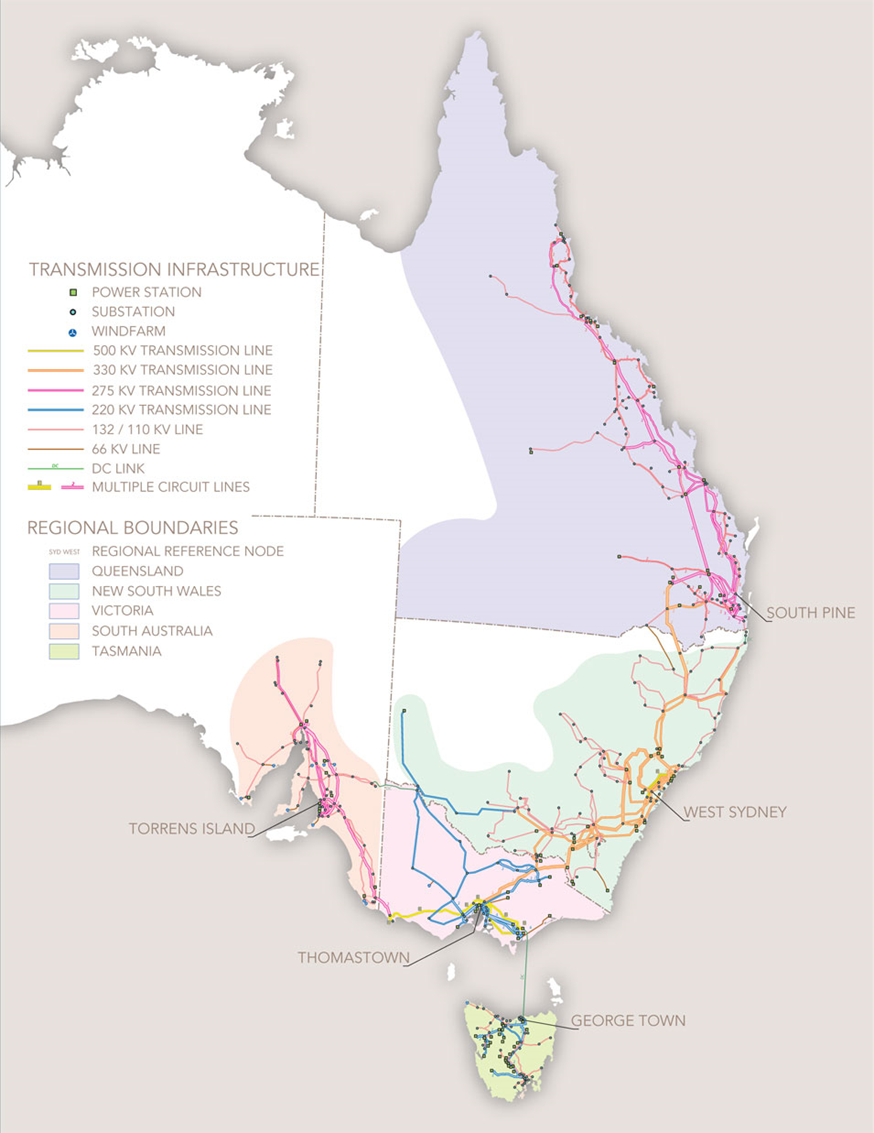
\includegraphics[width=0.8\textwidth,height=\textheight]{source/figures/NEM.png}
\caption[The National Electricity Market (NEM)]{Regions/states and
transmission in the NEM. Source: Australian Energy Market Commission
(\protect\hyperlink{ref-australianenergymarketcommissionNationalElectricityMarket}{n.d.a})}\label{fig:NEM}
}
\end{figure}

The NEM is a single platform (real-time) energy-only market with no
explicit capacity mechanisms. Unit commitment is managed by market
participants, who must submit resource-specific offers for energy and
Frequency Control Ancillary Services (FCAS) capacity in price-quantity
pairs the day before delivery. These offers are subsequently used in a
pre-dispatch process, which provides forecasted market information
(e.g.~generation and demand, interconnector flows, prices, etc.) to
market participants. While prices in submitted offers are fixed,
participants may change the energy volumes in their offer up to a few
minutes before the delivery dispatch interval commences. As the NEM is
single-sided, security-constrained economic dispatch is run every five
minute to meet forecast demand at least cost, subject to network and
security constraints. Much like ISO/RTO markets, energy and FCAS markets
are co-optimised with respect to technical feasibility and cost
(\protect\hyperlink{ref-australianenergymarketoperatorDispatchStandardOperating2019}{Australian
Energy Market Operator, 2021c},
\protect\hyperlink{ref-australianenergymarketoperatorFCASModelNEMDE2017}{2017b}).
Real-time dispatch produces zonal marginal prices for energy and FCAS,
which form the basis for market settlement in each of the NEM's regions.

\hypertarget{fcas-markets}{%
\subsection{FCAS markets}\label{fcas-markets}}

The NEM's competitive FCAS markets consist of eight separate raise and
lower FCAS products that can be classed as regulation FCAS or
contingency FCAS, with the former responsible for control when frequency
is within the normal operating frequency band (NOFB) and the latter for
when frequency deviates outside the NOFB after an event (see
Table~\ref{tbl:fcs-fcas}). This is similar to arrangements in many
ISO/RTO markets, where FCS are divided into event and non-event reserves
(\protect\hyperlink{ref-elaOperatingReservesVariable2011}{Ela et al.,
2011}).

Security-constrained economic dispatch includes system-wide and regional
FCAS requirement constraints. Regulation and contingency FCAS are
typically procured for and from all regions of the NEM in the absence of
binding local constraints. Local requirements for FCAS procurement apply
to Tasmania and to the other regions of the NEM if they experience
network constraints, are at risk of separation or when
islanded\footnote{From 2015-2019, the Tasmanian and mainland contingency
  FCAS markets were separated on average for 40\% of the time due to the
  technical limitations of the high voltage DC interconnector
  (\protect\hyperlink{ref-ghdadvisoryGHDReportTasNetworks2019}{GHD
  Advisory, 2019}). However, if the interconnector flow is within the
  appropriate operating envelope, NEM-wide FCAS procurement is possible
  as the interconnector's frequency controller enables FCAS transfer
  between the mainland and Tasmania
  (\protect\hyperlink{ref-australianenergymarketoperatorInterconnectorCapabilitiesNational2017}{Australian
  Energy Market Operator, 2017c}).}
(\protect\hyperlink{ref-australianenergymarketoperatorConstraintImplementationGuidelines2015}{Australian
Energy Market Operator, 2015a},
\protect\hyperlink{ref-australianenergymarketoperatorConstraintFormulationGuidelines2010}{2010}).
Prices are calculated for each region of the NEM based on the sum of the
shadow prices of local and system-wide constraints and FCAS costs are
allocated to market participants based on a "Causer Pays" principle,
which bears similarities to imbalance penalties in European markets
(\protect\hyperlink{ref-australianenergymarketoperatorGuideAncillaryServices2015}{Australian
Energy Market Operator, 2015b}). FCAS providers are paid for enablement
(capacity provision) regardless of whether their capacity is activated
(\protect\hyperlink{ref-australianenergymarketoperatorGuideAncillaryServices2015}{Australian
Energy Market Operator, 2015b};
\protect\hyperlink{ref-rieszFrequencyControlAncillary2015}{Riesz et al.,
2015};
\protect\hyperlink{ref-thorncraftExperienceMarketbasedAncillary2007}{Thorncraft
and Outhred, 2007}).

For a resource to provide FCAS, it must meet pre-qualification criteria
and undergo a registration process. Historically, FCAS was provided by
thermal generation (predominantly coal and some gas), hydropower
generation and some large loads, such as hydropower pumps and an
aluminium smelter, as only resources associated with wholesale energy
market participants were permitted to offer FCAS. In 2017, the first
battery energy storage system (BESS) in the NEM began to offer FCAS and
market reform enabled demand response (DR) aggregators to offer
contingency FCAS without participating in the energy market
(\protect\hyperlink{ref-aureconLargeScaleBatteryStorage2019}{Aurecon,
2019};
\protect\hyperlink{ref-australianenergymarketcommissionNationalElectricityAmendment2016}{Australian
Energy Market Commission, 2016}). In recent years, new FCAS market
entrants have included several DR aggregators, new BESS, distributed
PV-battery virtual power plants and wind farms (the latter two through
trials)
(\protect\hyperlink{ref-aureconLargeScaleBatteryStorage2019}{Aurecon,
2019};
\protect\hyperlink{ref-australianenergymarketoperatorAEMOVirtualPower2021}{Australian
Energy Market Operator, 2021d};
\protect\hyperlink{ref-australianenergyregulatorStateEnergyMarket2021}{Australian
Energy Regulator, 2021}). However, these new entrants tend to offer
smaller volumes and there are still relatively few FCAS providers in the
NEM, with no single FCAS product having more than 30 providers across
the system or 8 providers in any one region
(\protect\hyperlink{ref-australianenergyregulatorStateEnergyMarket2021}{Australian
Energy Regulator, 2021}).

\blandscape

\def\pandoctableshortcapt{Frequency control ancillary services in the
NEM}

\hypertarget{tbl:fcs-fcas}{}
\begin{longtable}[]{@{}
  >{\raggedright\arraybackslash}m{(\columnwidth - 6\tabcolsep) * \real{0.2182}}
  >{\raggedright\arraybackslash}m{(\columnwidth - 6\tabcolsep) * \real{0.2606}}
  >{\raggedright\arraybackslash}m{(\columnwidth - 6\tabcolsep) * \real{0.2667}}
  >{\raggedright\arraybackslash}m{(\columnwidth - 6\tabcolsep) * \real{0.2424}}@{}}
\caption[Frequency control ancillary services in the
NEM]{\label{tbl:fcs-fcas}Frequency control ancillary services in the
National Electricity Market. Sources: Thorncraft and Outhred
(\protect\hyperlink{ref-thorncraftExperienceMarketbasedAncillary2007}{2007}),
Riesz et al.
(\protect\hyperlink{ref-rieszFrequencyControlAncillary2015}{2015}),
Australian Energy Market Operator
(\protect\hyperlink{ref-australianenergymarketoperatorFastFrequencyResponse2017}{2017a}),
Australian Energy Market Operator
(\protect\hyperlink{ref-australianenergymarketoperatorConstraintFormulationGuidelines2010}{2010}),
Australian Energy Market Operator
(\protect\hyperlink{ref-australianenergymarketoperatorConstraintImplementationGuidelines2015}{2015a}),
Australian Energy Market Operator
(\protect\hyperlink{ref-australianenergymarketoperatorGuideAncillaryServices2015}{2015b}),
Australian Energy Market Operator
(\protect\hyperlink{ref-australianenergymarketoperatorPowerSystemRequirements2020}{2020c}).}\tabularnewline
\toprule\noalign{}
\begin{minipage}[b]{\linewidth}\raggedright
Product
\end{minipage} & \begin{minipage}[b]{\linewidth}\raggedright
Control action
\end{minipage} & \begin{minipage}[b]{\linewidth}\raggedright
Procurement
\end{minipage} & \begin{minipage}[b]{\linewidth}\raggedright
Timeframe
\end{minipage} \\
\midrule\noalign{}
\endfirsthead
\toprule\noalign{}
\begin{minipage}[b]{\linewidth}\raggedright
Product
\end{minipage} & \begin{minipage}[b]{\linewidth}\raggedright
Control action
\end{minipage} & \begin{minipage}[b]{\linewidth}\raggedright
Procurement
\end{minipage} & \begin{minipage}[b]{\linewidth}\raggedright
Timeframe
\end{minipage} \\
\midrule\noalign{}
\endhead
\bottomrule\noalign{}
\endlastfoot
Regulation (raise \& lower) & Centralised control through AEMO Automatic
Generation Control (AGC), which adjusts unit set points & Minimum
capacity enablement with dynamic additional reserve setting based on
time error for every dispatch interval & Unit set points adjusted by AGC
every 4-s over dispatch interval \\
6-s contingency (fast raise \& lower) & \multirow{2}{=}{Decentralised
control response to locally-measured frequency, typically delivered
through droop settings in governors or inverters or frequency-responsive
loads (raise only)} & \multirow{2}{=}{Capacity enablement based on size
of largest generator (raise) or load block (lower), minus assumed load
relief for every dispatch interval} & Full response delivered by 6-s
after frequency has left NOFB and orderly transition to 60-s service \\
60-s contingency (slow raise \& lower) & & & Full response delivered by
60-s after frequency has left NOFB and orderly transition to 5-min
service \\
5-min contingency (delayed raise \& lower) & Response pre-configured by
AEMO but triggered in response to locally-measured frequency. Typically
consists of unit control systems increasing or decreasing set points
with sustained frequency deviations & Capacity enablement based on size
of largest generator (raise) or load block (lower), minus assumed load
relief and corresponding Regulation FCAS procurement for every dispatch
interval & Full response delivered by 5-min after frequency has left
NOFB and sustained until frequency returns to NOFB or 10-min has
elapsed \\
\end{longtable}

\let\pandoctableshortcapt\relax

\elandscape

\hypertarget{nem-operation-and-governance}{%
\subsection{NEM operation and
governance}\label{nem-operation-and-governance}}

The Australian Energy Market Operator (AEMO) is responsible for the
operation of the market and power system in the NEM in accordance with
the National Electricity Rules (NER). They act as a single buyer of
dynamically-determined volumes of FCS. The Australian Energy Market
Commission (AEMC) is responsible for making or amending rules for the
NEM. Both AEMO and the AEMC provide operational and strategic advice to
the Energy Security Board (ESB), which is responsible for coordinating
market oversight and longer-term reform such as the ongoing post-2025
NEM market design framework. As the market regulator, the Australian
Energy Regulator (AER) monitors compliance with and enforces the NER.

\hypertarget{challenges-to-frequency-control-posed-by-vre-and-ibr}{%
\subsection{Challenges to frequency control posed by VRE and
IBR}\label{challenges-to-frequency-control-posed-by-vre-and-ibr}}

The rapid pace at which IBR have entered the NEM was preceded by the
exit of FCAS-capable synchronous generation
(Figure~\ref{fig:entry_exit}). Many of these IBR do not currently offer
FCAS or any meaningful frequency response to deviations other than the
most extreme. Furthermore, though updated equipment standards require
distributed IBR to ride-through and/or respond to certain frequency
deviations, some inverter models have been found to be non-compliant and
there is still a significant number of legacy systems in the NEM
(\protect\hyperlink{ref-australianenergymarketoperatorBehaviourDistributedResources2021}{Australian
Energy Market Operator, 2021e};
\protect\hyperlink{ref-stringerConsumerLedTransitionAustralia2020}{Stringer
et al., 2020}).

\begin{figure}
\hypertarget{fig:entry_exit}{%
\centering
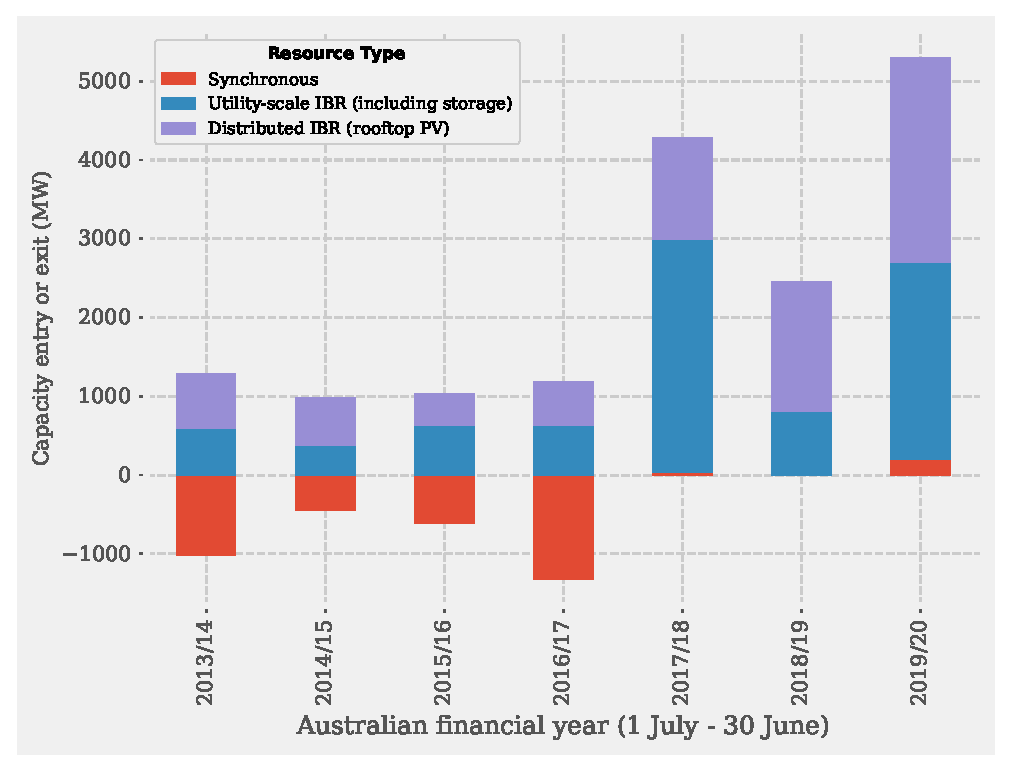
\includegraphics{source/figures/synchronous_ibr_entry_exit.eps}
\caption[Entry and exit of generation capacity in the NEM between
2013/14 and 2019/20]{Entry (of IBR) and exit (of synchronous generation)
capacity in the NEM between Australian financial years 2013/14 and
2019/20. Data source: Australian Energy Market Commission
(\protect\hyperlink{ref-australianenergymarketcommissionAnnualMarketPerformance2020}{2020a}).}\label{fig:entry_exit}
}
\end{figure}

The challenges that VRE and other IBR pose to frequency control have
been exacerbated by the NEM's network topology. Limited interconnection
between regions reduces the NEM's cross-regional balancing capabilities
and increases the likelihood of synchronous area separation following
power system events, a consequence of which is that local requirements
for FCAS may apply
(\protect\hyperlink{ref-australianenergymarketoperatorMaintainingPowerSystem2019}{Australian
Energy Market Operator, 2019a}). Furthermore, correlated variability and
uncertainty can arise from intensive development of similar
utility-scale VRE in areas with good wind or solar resources (as might
occur in the Renewable Energy Zones identified by AEMO's least-regrets
transmission planning study
(\protect\hyperlink{ref-australianenergymarketoperator2020IntegratedSystem2020}{Australian
Energy Market Operator, 2020d})). This is also an issue at the
distribution level given the significant installed capacities of rooftop
solar PV located within proximity of one another in suburban areas
(\protect\hyperlink{ref-australianenergymarketoperatorEnduringPrimaryFrequency2021}{Australian
Energy Market Operator, 2021f}).

\hypertarget{features-of-nem-frequency-control-arrangements}{%
\subsection{Features of NEM frequency control
arrangements}\label{features-of-nem-frequency-control-arrangements}}

Below, we highlight some noteworthy features of the NEM's frequency
control arrangements that complement or contrast previous analyses in
Thorncraft and Outhred
(\protect\hyperlink{ref-thorncraftExperienceMarketbasedAncillary2007}{2007}),
Riesz et al.
(\protect\hyperlink{ref-rieszFrequencyControlAncillary2015}{2015}) and
Thorncraft et al.
(\protect\hyperlink{ref-thorncraftMarketbasedAncillaryServices2008}{2008}).

\hypertarget{control-mechanisms}{%
\subsubsection{Control mechanisms:}\label{control-mechanisms}}

\begin{itemize}
\tightlist
\item
  There is no explicit TFR FCS in the NEM. Security-constrained economic
  dispatch is run every five minutes and is expected to relieve PFR and
  SFR and address supply-demand imbalances
  (\protect\hyperlink{ref-australianenergymarketoperatorPowerSystemRequirements2020}{Australian
  Energy Market Operator, 2020c}).
\item
  PFR from contingency FCAS is only required to respond to frequency
  deviations outside the NOFB (50 \(\pm\) 0.15 Hz). When FCAS markets
  were implemented in the NEM in 2001, mandatory PFR around a tight
  deadband of \(\pm\) 50 mHz was removed from the NER
  (\protect\hyperlink{ref-australianenergymarketoperatorElectricityRuleChange2019}{Australian
  Energy Market Operator, 2019b}). Since then and prior to 2020, there
  was no explicit procurement or requirement for tight-deadband PFR
  provision within the NOFB. The decline in the provision of
  tight-deadband PFR in the NEM is discussed further in
  Section~\ref{sec:fcs-pfr}.
\item
  The mainland synchronous area is controlled as one balancing area by
  AEMO's AGC (i.e.~no tie-line biased SFR) despite limited
  interconnection between adjacent regions
  (\protect\hyperlink{ref-australianenergymarketoperatorAEMCFrequencyControl2018}{Australian
  Energy Market Operator, 2018a}). AGC control performance is discussed
  further in Section~\ref{sec:fcs-regulation}.
\end{itemize}

\hypertarget{market-based-mechanisms}{%
\subsubsection{Market-based mechanisms:}\label{market-based-mechanisms}}

\begin{itemize}
\tightlist
\item
  There are relatively few limits imposed on FCAS participation. FCAS
  can be provided by any technology through variable, switched or hybrid
  controllers
  (\protect\hyperlink{ref-australianenergymarketoperatorMarketAncillaryService2020a}{Australian
  Energy Market Operator, 2020e}). Furthermore, regulation and
  contingency FCAS products are unbundled into raise and lower services,
  and contingency FCAS products are unbundled based on response time.
  All of these features improve the potential for participation and
  competition in FCAS markets, though market participants can and often
  are enabled to provide multiple FCAS.
\item
  FCAS unbundling has enabled a `Causer Pays' cost allocation framework.
  Raise contingency FCAS costs, which are incurred as insurance for the
  failure of a generator, are distributed amongst generators in
  proportion to their generation in the trading interval. Similarly,
  lower contingency FCAS costs are distributed amongst loads based on
  their consumption in a trading interval. A complex methodology is used
  to calculate monthly, portfolio-wide Causer Pays contribution factors
  (outlined in Australian Energy Market Operator
  (\protect\hyperlink{ref-australianenergymarketoperatorRegulationFCASContribution2018a}{2018b})
  and summarised in Riesz et al.
  (\protect\hyperlink{ref-rieszFrequencyControlAncillary2015}{2015}))
  that determine how regulation FCAS costs are allocated to market
  participants. We discuss the issues associated with this methodology
  in Section~\ref{sec:fcs-regulation}.
\item
  The NEM co-optimises FCAS that respond within similar timeframes. In
  the absence of constraints, the volume of 5-minute delayed contingency
  FCAS procured is reduced by the volume of regulation FCAS enabled
  (\protect\hyperlink{ref-australianenergymarketoperatorConstraintFormulationGuidelines2010}{Australian
  Energy Market Operator, 2010}).
\end{itemize}

\hypertarget{regulatory-mechanisms}{%
\subsubsection{Regulatory mechanisms:}\label{regulatory-mechanisms}}

\begin{itemize}
\item
  Connecting utility-scale generators negotiate the frequency response
  capability of their plant between a minimum access standard and an
  automatic access standard, the latter guaranteeing network access to
  the applicant. A suite of generator standards for frequency response
  were added to the NER in October 2018 and apply to any
  newly-connecting generation. These standards include minimum frequency
  disturbance ride-through times, automatic generation output reduction
  following extreme over-frequency events and the capability to operate
  in a frequency response mode with a proportional response\footnote{In
    addition to these standards, newly-connected generation may install
    a synchronous condenser under the `do no harm' requirements outlined
    in the NER if they are determined to have an adverse impact on
    system strength. Particularly when fitted with a rotating mass or
    flywheel, these synchronous condensers can also provide inertial
    response
    (\protect\hyperlink{ref-australianenergymarketoperatorSystemStrengthNEM2020}{Australian
    Energy Market Operator, 2020f}).}
  (\protect\hyperlink{ref-australianenergymarketcommissionGeneratorTechnicalPerformance2018}{Australian
  Energy Market Commission, 2018a}).
\item
  Transmission Network Service Providers (TNSPs) are required to address
  any inertia shortfalls identified by AEMO within the NEM region in
  which they build, maintain, plan and operate the transmission network.
  AEMO's assessment considers whether an islanded region can be securely
  operated following a contingency event. Shortfalls can be reduced by
  special protection schemes (e.g.~disconnection of load following
  interconnector trip) and the provision of FFR, but they must
  ultimately be met by providers of inertial response
  (\protect\hyperlink{ref-australianenergymarketoperatorNoticeSouthAustralia2020}{Australian
  Energy Market Operator, 2020g},
  \protect\hyperlink{ref-australianenergymarketoperatorInertiaRequirementsMethodology2018}{2018c}).
\end{itemize}

\hypertarget{sec:fcs-insights}{%
\section{Insights from the National Electricity
Market}\label{sec:fcs-insights}}

In light of existing challenges and those posed by energy transition,
effective and efficient frequency control arrangements should enable
sufficient FCS to be procured across timeframes and strike the
appropriate balance between efficiency and robustness. In the following
sections, we review issues associated with two core elements of the
NEM's frequency control hierarchy (i.e.~PFR and SFR), assess their
physical and economic performance and outline reform underway. Drawing
on developments in the NEM and our review of arrangements in North
America and Europe, we then discuss the merits and flaws of regulatory
and market-based mechanisms with respect to sufficiency and efficiency.
We conclude by offering insights that could serve as design principles
for jurisdictions revisiting their frequency control arrangements during
energy transition.

\hypertarget{sec:fcs-pfr}{%
\section{Declining tight-deadband primary frequency
response}\label{sec:fcs-pfr}}

When FCAS markets were implemented in 2001, mandatory tight-deadband PFR
was superseded by two types of PFR: voluntary PFR within the NOFB and
competitive procurement for PFR outside the NOFB in the form of
contingency FCAS
(\protect\hyperlink{ref-australianenergymarketoperatorElectricityRuleChange2019}{Australian
Energy Market Operator, 2019b}).

As such, the NEM's frequency control scheme deviated from what has been
argued to be international best practice as it only explicitly specified
and procured wide-deadband PFR (i.e.~deadband of \(\pm\) 150 mHz)
(\protect\hyperlink{ref-australianenergymarketoperatorElectricityRuleChange2019}{Australian
Energy Market Operator, 2019b}). In contrast, ENTSO-E specifies that PFR
providers have a deadband no greater than \(\pm\) 10-15 mHz depending on
the control area
(\protect\hyperlink{ref-europeannetworkoftransmissionsystemoperatorsforelectricityentso-eNetworkCodeLoadFrequency2013}{European
Network of Transmission System Operators for Electricity, 2013}) and
FERC Order 842 mandates all newly-connecting generation in US
interconnections to operate frequency-responsive control equipment with
maximum deadbands of \(\pm\) 36 mHz
(\protect\hyperlink{ref-federalenergyregulatorycommissionfercOrderNo8422018}{Federal
Energy Regulatory Commission, 2018}).

In recent years in the NEM, the lack of an incentive or requirement for
tight-deadband PFR and perceived disincentives to its provision (through
Causer Pays contribution factors discussed further in
Section~\ref{sec:fcs-regulation}) has led to many synchronous generators
that once provided tight-deadband PFR to widen deadbands or install
control systems that block or dampen PFR from the speed governor within
the NOFB
(\protect\hyperlink{ref-australianenergymarketcommissionMandatoryPrimaryFrequency2020}{Australian
Energy Market Commission, 2020b}). Furthermore, many VRE generators were
deployed in the NEM and connected with inverter control systems that
were unresponsive to any frequency deviations other than the most
serious.

The extent to which tight-deadband PFR provision had declined in the NEM
and the consequences of this became clear to AEMO following a major
power system incident on the 25\textsuperscript{th} of August 2018
(\protect\hyperlink{ref-australianenergymarketoperatorFinalReportQueensland2019}{Australian
Energy Market Operator, 2019c}). Prior to the event, the QLD region was
exporting \(\sim\) 900 MW to the rest of the NEM. Around 13:11:41,
lightning strikes at the QLD-NSW interconnector resulted in the QLD
region being separated from the rest of the NEM with excess supply. The
SA region was exporting \(\sim\) 200 MW prior to the event and following
QLD's separation, this increased by more than 200 MW in response to
under-frequency. The sudden increase in active power flow triggered an
emergency scheme that disconnected SA from the NSW-VIC synchronous area,
resulting in local over-frequency.

There were diverse responses from various generators following the
double separation event. While many synchronous generators provided some
form of PFR though not enabled for FCAS, their response was withdrawn by
their load controllers in several cases so that the unit could return to
its dispatch target (e.g.~green and pink lines in top frame of
Figure~\ref{fig:plant_responses}). Wind and solar farms were either
unresponsive, tripped due to protection settings in their inverters, or
reduced their active power output in line with performance standards
negotiated in their connection agreements (middle and bottom frames in
Figure~\ref{fig:plant_responses}). AEMO attributed slow frequency
recovery and under-frequency load shedding in NSW and VIC to
insufficient PFR from generators and a lack of appropriate contingency
FCAS within the islanded regions. Over 50\% of fast and slow raise
contingency FCAS needed in NSW-VIC was enabled in SA and QLD, whilst QLD
had no lower FCAS enabled to respond to over-frequency\footnote{AEMO is
  currently investigating appropriate regional requirements for FCAS,
  particularly for contingency FCAS in the terminal regions of QLD and
  SA
  (\protect\hyperlink{ref-australianenergymarketoperatorRenewableIntegrationStudy2020b}{Australian
  Energy Market Operator, 2020h},
  \protect\hyperlink{ref-australianenergymarketoperatorElectricityRuleChange2019a}{2019d}).}
(\protect\hyperlink{ref-australianenergymarketoperatorFinalReportQueensland2019}{Australian
Energy Market Operator, 2019c}).

\begin{figure}
\hypertarget{fig:plant_responses}{%
\centering
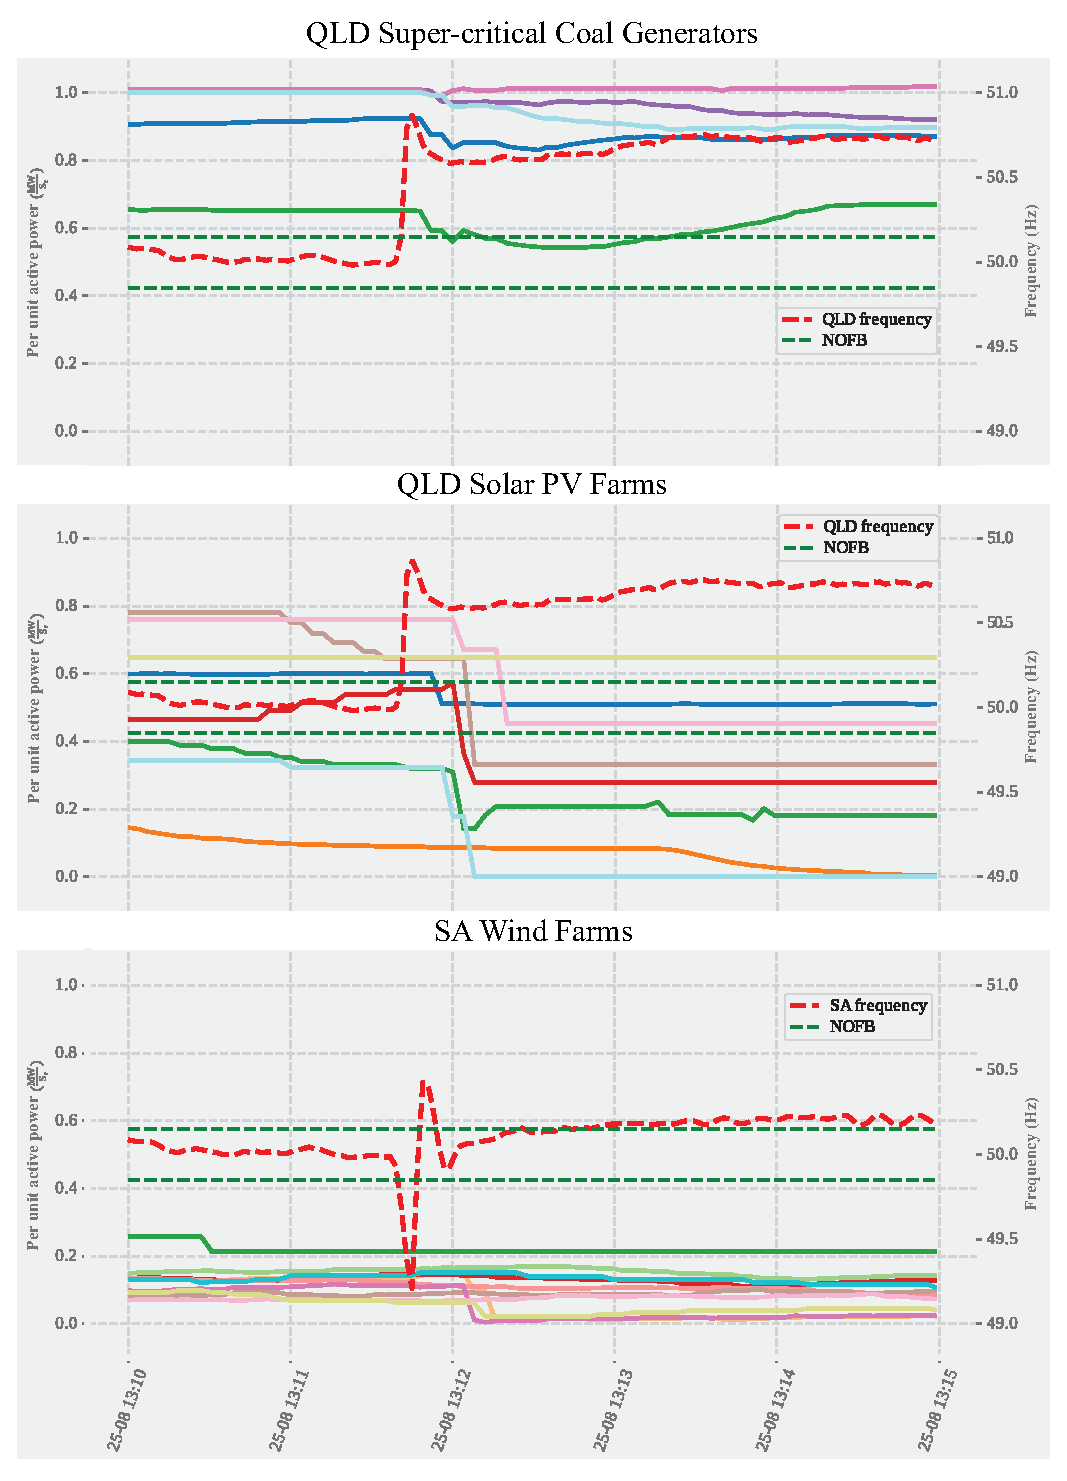
\includegraphics{source/figures/all_responses_25082018.eps}
\caption[Response of different generation technologies to power system
events on the 25th of August, 2018]{Active power output of QLD
super-critical coal generators (top), SA solar PV farms (middle) and SA
wind farms (bottom). The response of an individual generator is denoted
by solid lines (obtained from 4-second AEMO SCADA data using NEMOSIS
(\protect\hyperlink{ref-gormanNEMOSISNEMOpen2018}{Gorman et al.,
2018})). None of these generators are enabled for FCAS. The red dashed
line in each frame is the regional frequency as measured by high-speed
(1-second) phasor measurement units.}\label{fig:plant_responses}
}
\end{figure}

Prior to this incident, deteriorating control of frequency within the
NOFB was of concern to AEMO and the AEMC, and trials and investigations
were recommended to inform the design of an incentive for tight-deadband
PFR provision
(\protect\hyperlink{ref-australianenergymarketcommissionFrequencyControlFrameworks2018}{Australian
Energy Market Commission, 2018b}). However, this separation event
demonstrated the ``urgent need for regulatory changes to arrest the
ongoing decline in frequency performance in the NEM'' and to enhance
``the resilience of the NEM to similar major disturbances'', with AEMO
submitting a rule change proposal for all capable generators in the NEM
to provide mandatory PFR with a maximum deadband of \(\pm\) 0.015 Hz
(i.e.~10\% of the NOFB)
(\protect\hyperlink{ref-australianenergymarketoperatorElectricityRuleChange2019}{Australian
Energy Market Operator, 2019b}).

This rule was initially incorporated into the NER in 2020 as a temporary
arrangement through the addition of a ``sunset'' after three years to
demonstrate the AEMC's commitment to investigating incentives or
market-based mechanisms for tight-deadband PFR
(\protect\hyperlink{ref-australianenergymarketcommissionMandatoryPrimaryFrequency2020}{Australian
Energy Market Commission, 2020b},
\protect\hyperlink{ref-australianenergymarketcommissionFrequencyControlRule2020}{2020c}).
AEMO has specified PFR settings, including maximum droop and response
time, but is unable to require generation to reserve headroom for PFR
(\protect\hyperlink{ref-australianenergymarketoperatorInterimPrimaryFrequency2020}{Australian
Energy Market Operator, 2020i}).

\hypertarget{sec:fcs-regulation}{%
\section{Performance and efficiency issues of regulation
services}\label{sec:fcs-regulation}}

For SFR provided by regulation FCAS within the NOFB to be effective, the
dynamics of the system need to accommodate slower SFR control action and
the centralised secondary controller (in the NEM, AEMO's AGC) needs to
be properly configured. Prior to the introduction of mandatory PFR in
the NEM, AEMO observed no significant improvement in NOFB frequency
stability despite several increases in the minimum volumes procured for
regulation FCAS in 2019
(\protect\hyperlink{ref-australianenergymarketoperatorElectricityRuleChange2019}{Australian
Energy Market Operator, 2019b}). This is likely due to:

\begin{itemize}
\tightlist
\item
  A lack of fast and decentralised tight-deadband PFR supporting slower
  SFR;
\item
  Inappropriate control signals being calculated within the AGC due to
  the use of rate limiters to account for ramping constraints, signal
  filtering and generator controller models that do not accurately
  reflect a unit's frequency response
  (\protect\hyperlink{ref-digsilentReviewFrequencyControl2017}{DIgSILENT,
  2017}). The latter is the consequence of an absence of control
  coordination between market participants and AEMO; and
\item
  Variable communication delays between individual unit controllers and
  AEMO's AGC system, and disparate response times from generators.
\end{itemize}

Furthermore, the control of all mainland regions as one balancing area
can be problematic in the event of separation. AGC control of regulation
FCAS enabled in islanded regions may exacerbate local frequency
deviations when responding to the AGC frequency reference. This was the
case during the double separation event on the 25\textsuperscript{th} of
August 2018, in which the AGC instructed raise regulation FCAS
generators in QLD and SA to respond to under-frequency in the AGC
frequency reference despite local over-frequency
(Figure~\ref{fig:regional_freq}). Such incorrect control action can
occur until AEMO is able to manually reconfigure the AGC to treat each
island as a control area - a process which can take up to 15 minutes
(\protect\hyperlink{ref-australianenergymarketoperatorFinalReportQueensland2019}{Australian
Energy Market Operator, 2019c}) .

\begin{figure}
\hypertarget{fig:regional_freq}{%
\centering
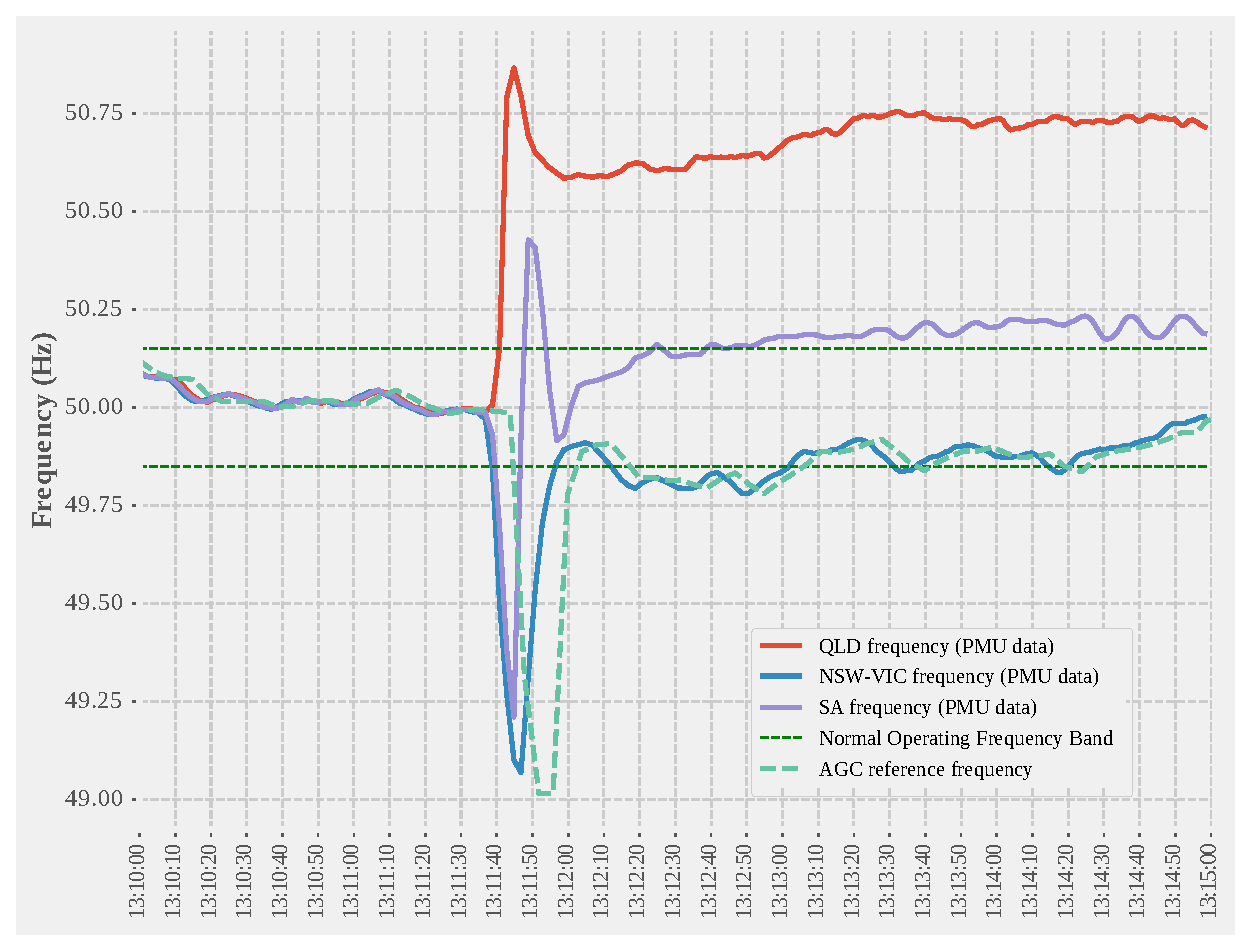
\includegraphics{source/figures/regional_SCADA_frequencies.eps}
\caption[System frequency (as registered by phasor measurement units and
AEMO\textquotesingle s AGC) during the power system event on the
25\^{}th\^{} of August, 2018]{Regional phasor measurement unit frequency
data and AGC reference frequency data from AEMO's NSW control centre
(obtained using NEMOSIS
(\protect\hyperlink{ref-gormanNEMOSISNEMOpen2018}{Gorman et al., 2018}))
during the power system event on the 25\textsuperscript{th} of August,
2018. Note that the AGC reference frequency deviates in the opposite
direction to local frequency in QLD and SA.}\label{fig:regional_freq}
}
\end{figure}

Over time, inefficiencies in regulation FCAS procurement and
cost-allocation have also become apparent. Regulation FCAS procurement
in the NEM is dynamic beyond a minimum volume, but the dynamic component
is based on the system time error
(\protect\hyperlink{ref-australianenergymarketoperatorConstraintImplementationGuidelines2015}{Australian
Energy Market Operator, 2015a}). Time error control is largely
unnecessary as modern clocks no longer rely on power system frequency to
keep the time
(\protect\hyperlink{ref-reboursFundamentalDesignIssues2007}{Y. Rebours
et al., 2007}). Furthermore, whilst AEMO is required to control the NEM
within certain time error limits, these have been relaxed in recent
years
(\protect\hyperlink{ref-australianenergymarketcommissionreliabilitypanelStageOneFinal2017}{Australian
Energy Market Commission Reliability Panel, 2017}). Given that time
error is no longer prioritised as a control objective, dynamic
regulation FCAS procurement based on better measures of sustained
frequency deviation (e.g.~mean absolute error as suggested by Riesz et
al. (\protect\hyperlink{ref-rieszFrequencyControlAncillary2015}{2015}))
and/or a modelled distribution of potential intra-dispatch ramp
uncertainty may be more suitable.

Regulation FCAS costs are allocated to market participants based on
their contribution factor, a calculation which represents the extent to
which the participant has contributed to the need for regulation FCAS
through a deviation from a dispatch trajectory. Though the calculation
methodology assigns weights to a generator or load's dispatch trajectory
deviation based on the AGC regulation direction and mileage requirement
every 4 seconds, the disincentive for dispatch deviation suffers from a
disconnect to causation. This is because the contribution factors of a
generator or load are averaged over a 5-minute dispatch interval, summed
over a 28-day period and then within a market participant's portfolio
(\protect\hyperlink{ref-australianenergymarketcommissionFrequencyControlFrameworks2018}{Australian
Energy Market Commission, 2018b};
\protect\hyperlink{ref-australianenergymarketoperatorRegulationFCASContribution2018a}{Australian
Energy Market Operator, 2018b};
\protect\hyperlink{ref-australianenergyregulatorIssuesPaperSemi2020}{Australian
Energy Regulator, 2020}).

Much like portfolio-based balancing in Europe, the aggregation of
contribution factors enables a market participant to offset antagonistic
deviations with assisting deviations (from the provision of
tight-deadband PFR) across its resources and time. However, the
complexity and opacity of the methodology and cost-allocation process
has contributed to the withdrawal of tight-deadband PFR in the NEM.
Several generators disabled governor response in the NOFB in the belief
that dispatch adherence alone will minimise Causer Pays liabilities
(\protect\hyperlink{ref-digsilentReviewFrequencyControl2017}{DIgSILENT,
2017}).

\hypertarget{nem-assessment-and-outlook}{%
\section{NEM assessment and outlook}\label{nem-assessment-and-outlook}}

Though the introduction of competitive FCAS markets in 2001 initially
resulted in significantly lower FCAS prices in the NEM
(\protect\hyperlink{ref-rieszFrequencyControlAncillary2015}{Riesz et
al., 2015};
\protect\hyperlink{ref-thorncraftExperienceMarketbasedAncillary2007}{Thorncraft
and Outhred, 2007}), volume-weighted average FCAS prices, particularly
those for raise regulation and contingency services, have increased
relative to the volume-weighted average energy price since 2016
(Figure~\ref{fig:raise_fcas_vwap}). Furthermore, the increases in
minimum regulation FCAS volumes and reductions in assumed load relief in
2019 have raised the procured volumes of regulation and contingency
FCAS, respectively. Together, these factors have contributed to higher
NEM-wide FCAS costs
(\protect\hyperlink{ref-australianenergymarketoperatorReviewNEMLoad2019}{Australian
Energy Market Operator, 2019e}). While quarterly FCAS costs were less
than 1\% of quarterly total NEM costs in 2015, 50\% of all quarters from
2017 to 2020 had FCAS costs that were between 1-2\% of total NEM cost
(\protect\hyperlink{ref-australianenergyregulatorStateEnergyMarket2021}{Australian
Energy Regulator, 2021}).

\begin{figure}
\hypertarget{fig:raise_fcas_vwap}{%
\centering
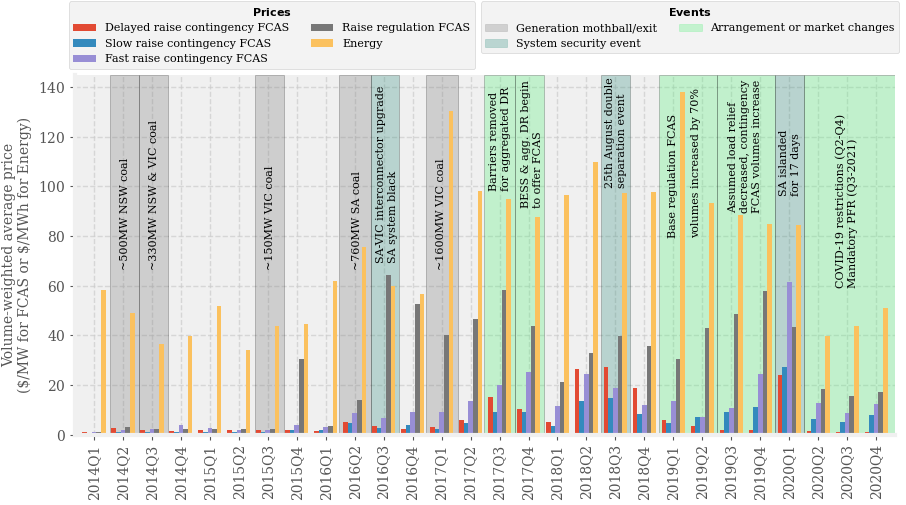
\includegraphics{source/figures/energy_raise_fcas_vwap_quarterly_2014_2020_v2.png}
\caption[Volume-weighted NEM-wide average quarterly prices for energy
and FCAS, 2014-2020]{Events and volume-weighted NEM-wide average
quarterly prices for energy, raise regulation FCAS and raise contingency
FCAS in the NEM. The entry of new albeit smaller FCAS providers in 2017
was preceded by the retirement of several large thermal generation. Q1
2020 FCAS prices were high due to local procurement in the SA region,
which was islanded for approximately two weeks. Note that while average
energy prices fell in Q2-Q4 in 2020 to levels previously seen in
2014-2015 (due to lower demand during COVID-19 lockdowns), FCAS prices
remained relatively high. Five-minute price and volume data obtained
using NEMOSIS (\protect\hyperlink{ref-gormanNEMOSISNEMOpen2018}{Gorman
et al., 2018}).}\label{fig:raise_fcas_vwap}
}
\end{figure}

Prior to the implementation of mandatory PFR, higher NEM FCAS costs were
arguably not accompanied by an improvement in frequency control
performance. Alongside deteriorating frequency control performance
within the NOFB (Figure~\ref{fig:nofb_freq_2005_2018}), AEMO has
expressed a loss of confidence in the NEM's resilience to complex power
system events, such as the double separation incident on the
25\textsuperscript{th} of August 2018
(\protect\hyperlink{ref-australianenergymarketoperatorElectricityRuleChange2019}{Australian
Energy Market Operator, 2019b}). These events are typically more severe
than the `credible' contingency events (i.e.~N-1 contingency) that
dictate the volume of contingency FCAS procured.

\begin{figure}
\hypertarget{fig:nofb_freq_2005_2018}{%
\centering
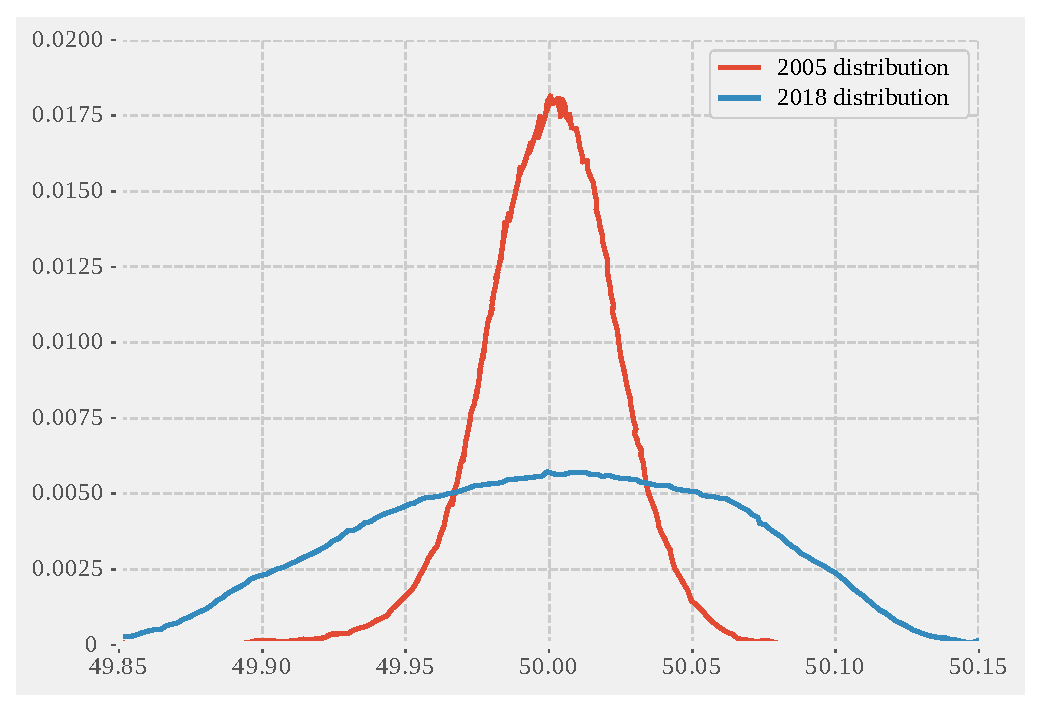
\includegraphics{source/figures/nem_nofb_frequency_2005_2018_digitised.eps}
\caption[NEM mainland frequency distributions, 2005 and 2018]{Normalised
distribution of mainland frequency within the NOFB in 2005 and 2018.
Reproduced from
(\protect\hyperlink{ref-australianenergymarketoperatorElectricityRuleChange2019a}{Australian
Energy Market Operator, 2019d})}\label{fig:nofb_freq_2005_2018}
}
\end{figure}

Since the implementation of the mandatory PFR, settings specified by
AEMO have been applied to a majority of large synchronous generators
(\(>\) 200MW) and some smaller synchronous generators. Despite the
absence of requirements for maintaining headroom and/or footroom,
preliminary analysis by AEMO\footnote{The ramp rate used in dispatch by
  AEMO is the lesser of a telemetered rate or a ramp rate submitted in a
  resource's offer for energy, and was obtained using NEMOSIS
  (\protect\hyperlink{ref-gormanNEMOSISNEMOpen2018}{Gorman et al.,
  2018}).} suggests that mandatory PFR has delivered better control of
frequency within the NOFB (see Figure~\ref{fig:mpfr_dist}) and reduced
excursions beyond the NOFB
(\protect\hyperlink{ref-australianenergymarketoperatorEnduringPrimaryFrequency2021}{Australian
Energy Market Operator, 2021f}). As a result of this initial success and
further technical advice provided by AEMO, the AEMC has indicated that
it intends to retain mandatory PFR at a tight-deadband following the
``sunset'' of the initial rule
(\protect\hyperlink{ref-australianenergymarketcommissionPrimaryFrequencyResponse2021}{Australian
Energy Market Commission, 2021a}).

\begin{figure}
\hypertarget{fig:mpfr_dist}{%
\centering
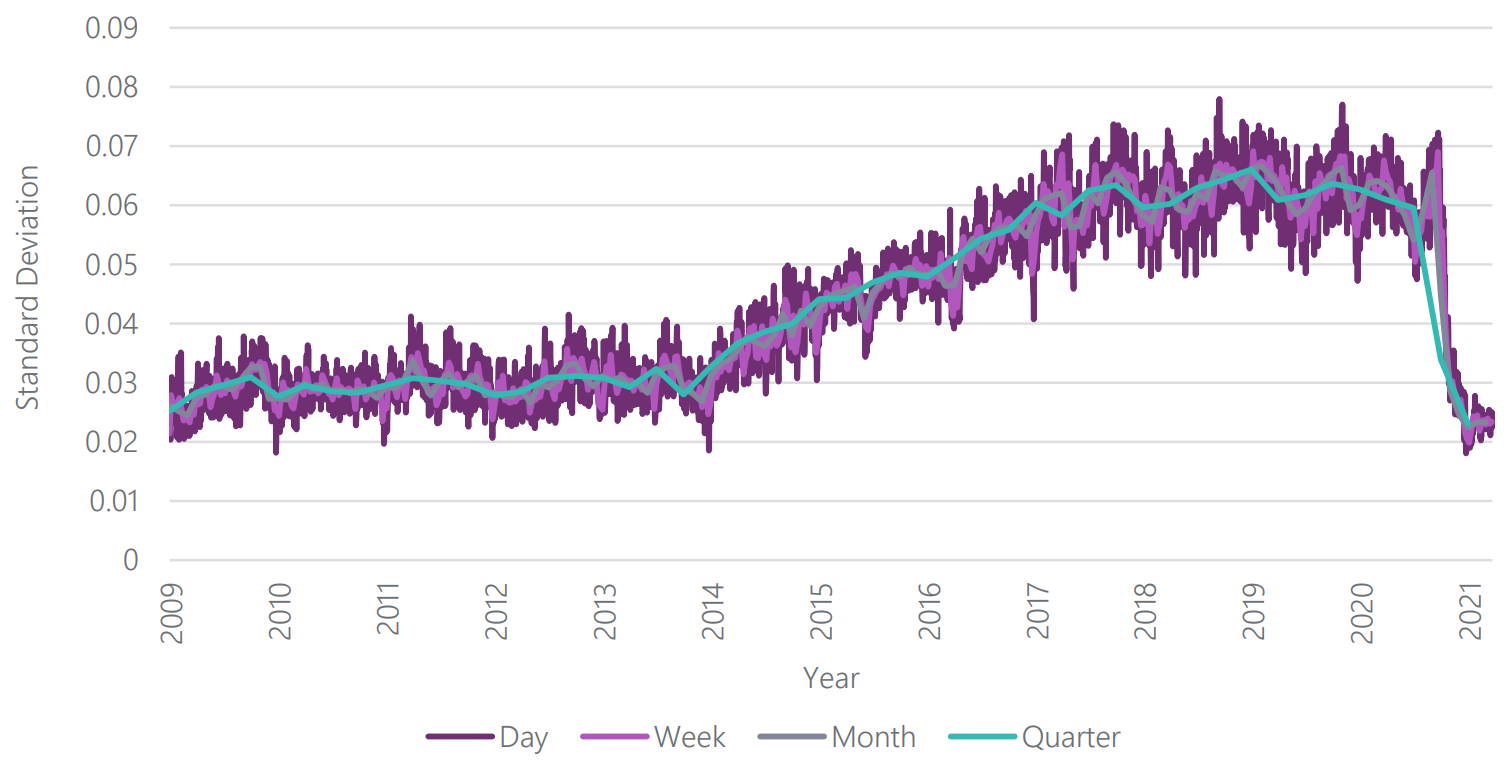
\includegraphics{source/figures/f_stddev_2009_2021.png}
\caption[Standard deviation of NEM mainland frequency from 2009 to
2021]{Standard deviation of mainland frequency grouped by each day,
week, month or quarter from 2009 to 2021. Some initial PFR setting
changes were made in late September 2020 and many generators moved to
final settings in late October 2020. Source: Australian Energy Market
Operator
(\protect\hyperlink{ref-australianenergymarketoperatorEnduringPrimaryFrequency2021}{2021f}).}\label{fig:mpfr_dist}
}
\end{figure}

However, this initial success may be a result of the headroom maintained
by these generators for risk management purposes (e.g.~defending
contract positions) and any headroom made available to the system
through the displacement of more expensive synchronous capacity by VRE.
Given that several large synchronous generators are expected to retire
in the coming decades
(\protect\hyperlink{ref-australianenergymarketoperator2020IntegratedSystem2020}{Australian
Energy Market Operator, 2020d}), continuing to rely on this ``free''
headroom (and any available footroom) into the future may reduce the
potential resilience benefits of widespread, tight-deadband PFR and
place a greater burden on generators that do reserve headroom and hence
respond. The AEMC is proposing to address this issue by paying resources
that provide assisting tight-deadband PFR (``double-siding'')
(\protect\hyperlink{ref-australianenergymarketcommissionPrimaryFrequencyResponse2021}{Australian
Energy Market Commission, 2021a}).

Presently, several other operational and market changes are being
considered or implemented with the goal of improving the effectiveness
of arrangements in the NEM. AEMO is investigating the use of dispatch
constraints to
(\protect\hyperlink{ref-australianenergymarketoperatorFrequencyControlWork2021}{Australian
Energy Market Operator, 2021g}):

\begin{itemize}
\tightlist
\item
  Procure contingency FCAS volumes based on system inertia;
\item
  Apply regional contingency and regulation FCAS requirements; and
\item
  To limit the amount of switched contingency FCAS procured. Switched
  FCAS has a number of limitations compared to governor-like control
  (\protect\hyperlink{ref-australianenergymarketoperatorRenewableIntegrationStudy2020c}{Australian
  Energy Market Operator, 2020b}).
\end{itemize}

These additional constraints will likely improve the effectiveness of
frequency control arrangements but may lead to higher FCAS costs. In
addition to these procurement changes, the AEMC has made a rule to
introduce raise and lower contingency markets for FFR by October 2023,
each with a likely response time of 1 second
(\protect\hyperlink{ref-australianenergymarketcommissionFastFrequencyResponse2021}{Australian
Energy Market Commission, 2021b};
\protect\hyperlink{ref-australianenergymarketoperatorFastFrequencyResponse2021}{Australian
Energy Market Operator, 2021h}). Whilst AEMO has highlighted that
potential stability issues and interconnector maloperation will need to
be managed (e.g.~through delivery caps or provision constraints)
(\protect\hyperlink{ref-australianenergymarketoperatorImplementationNationalElectricity2021}{Australian
Energy Market Operator, 2021i}), these FFR markets, along with the ESB's
proposals for short-term scheduling and/or procurement of inertial
response
(\protect\hyperlink{ref-energysecurityboardPost2025Market2021}{Energy
Security Board, 2021}), will likely improve AEMO's operational toolbox
for managing a low-inertia NEM.

\hypertarget{reactive-regulatory-requirements}{%
\subsection{Reactive regulatory
requirements}\label{reactive-regulatory-requirements}}

Despite a broad set of FCS markets, there is a high degree of reliance
on regulatory mechanisms in the NEM. Performance standards and mandatory
PFR enforced by connection requirements in the NEM have recently been
aligned with international grid-codes
(\protect\hyperlink{ref-robertsReviewInternationalGrid2018}{Roberts,
2018}). As argued by TNSPs and AEMO during the mandatory PFR rule change
process, near-universal widespread provision of frequency control should
lead to relatively low costs for individual participants and be
outweighed by greater visibility and certainty for AEMO alongside the
system-wide benefits of improved physical frequency control performance
(\protect\hyperlink{ref-australianenergymarketoperatorElectricityRuleChange2019}{Australian
Energy Market Operator, 2019b};
\protect\hyperlink{ref-dillonMandatoryPrimaryFrequency2019}{Dillon,
2019};
\protect\hyperlink{ref-hopwoodMandatoryPrimaryFrequency2019}{Hopwood,
2019}).

Regulatory mechanisms are ideal for mandating basic FCS capabilities as
a condition for access, which may reduce the need to procure more
specialised FCS, or where FCS faces significant barriers to efficient
price formation or unbundled procurement. The latter reasons are
particularly pertinent in the NEM. Current FCAS prices do not appear to
be incentivising FCS provision from the vast majority of VRE generators,
which have business models centred around energy provision
(\protect\hyperlink{ref-australianenergymarketcommissionReserveServicesNational2021}{Australian
Energy Market Commission, 2021c};
\protect\hyperlink{ref-meegahapolaPowerSystemStability2021}{Meegahapola
et al., 2021}). Furthermore, procuring inertial response is challenging
due to its inseparability from system strength provision and unit
commitment costs
(\protect\hyperlink{ref-billimoriaMarketDesignSystem2020}{Billimoria et
al., 2020}). With respect to these challenges, regulatory mechanisms in
the NEM have assisted in ensuring some level of frequency response from
most power system resources (e.g.~mandatory PFR) and improving the
ability of AEMO and TNSPs to coordinate the procurement of essential but
``lumpy'' FCS (e.g.~inertia shortfall mechanism).

While mechanisms such as mandatory PFR are likely to improve the
robustness of frequency control arrangements, it may be difficult for
other regulatory mechanisms to keep in step with changing physical
performance requirements in systems rapidly facing higher penetrations
of VRE and IBR. Regulatory mechanisms are often only updated after a
number of years to reduce the burden placed on connecting resources. As
such, they are slow to respond to changing capabilities and
requirements. This delay often makes new standards and requirements
reactive rather than proactive. For example, AEMO can only review
utility-scale generator technical performance standards every 5 years
(\protect\hyperlink{ref-australianenergymarketcommissionGeneratorTechnicalPerformance2018}{Australian
Energy Market Commission, 2018a}), a timeframe in which the solar PV
capacity installed in the NEM has more than quadrupled (2015-2020)
(\protect\hyperlink{ref-australianpvinstituteInstalledPVGeneration}{Australian
PV Institute, n.d.}).

Additional concerns with regulatory mechanisms include poor dynamic
efficiency and opaque
costs(\protect\hyperlink{ref-rieszFrequencyControlAncillary2015}{Riesz
et al., 2015}). In the absence of remuneration or incentives,
particularly those that are linked to the quality of frequency response,
there is no incentive to innovate or invest in higher-quality frequency
control capabilities
(\protect\hyperlink{ref-meegahapolaPowerSystemStability2021}{Meegahapola
et al., 2021}). Furthermore, cost opacity may lead to FCS provision
costs being internalised within other prices (e.g.~energy) by
participants and prevent the implementation of imbalance or dispatch
non-conformance disincentives through cost-allocation mechanisms.

\hypertarget{preference-for-market-based-arrangements}{%
\section{Preference for market-based
arrangements}\label{preference-for-market-based-arrangements}}

Since the establishment of the NEM, a competition norm has been
established, with markets being viewed as a key driver for delivering
the National Electricity Objective of ``efficient investment in, and
efficient operation and use of electricity services''
(\protect\hyperlink{ref-hainesEnvironmentalNormsElectricity2016}{Haines
and McConnell, 2016};
\protect\hyperlink{ref-macgillElectricityMarketNorms2020}{MacGill et
al., 2020}). This norm has pervaded all levels of participation and
governance in the NEM. Generator owners opposed the mandatory nature of
the mandatory PFR rule change on the basis that a lack of remuneration
was against market principles and that it would lead to economically
inefficient outcomes
(\protect\hyperlink{ref-rolfeMandatoryPrimaryFrequency2019}{Rolfe,
2019}; \protect\hyperlink{ref-scottMandatoryPrimaryFrequency2019}{Scott,
2019};
\protect\hyperlink{ref-skinnerMandatoryPrimaryFrequency2019}{Skinner,
2019}). AEMO did not include a headroom requirement in its proposal,
making the mandatory PFR rule change more palatable to market bodies and
participants. The AEMC, who have expressed a clear preference for
market-based approaches
(\protect\hyperlink{ref-australianenergymarketcommissionFrequencyControlFrameworks2018}{Australian
Energy Market Commission, 2018b}), included a ``sunset'' clause in their
initial decision to implement mandatory PFR. Furthermore, a market for
FFR will be implemented in 2023 and the ESB's post-2025 market design
process is considering new system services markets for inertial response
and TFR
(\protect\hyperlink{ref-energysecurityboardPost2025Market2021}{Energy
Security Board, 2021},
\protect\hyperlink{ref-energysecurityboardPost2025Market2020}{2020}).

If incentives or remuneration are designed correctly, markets can drive
short-run efficiency. Where required, they can also support investment
in FCS capability and assist a power system in achieving dynamically
efficient frequency control arrangements. However, in some cases, simply
introducing new FCS markets may serve as `patchwork' solutions to
existing control deficiencies and market failures. These deficiencies
and failures could be partially addressed by improving FCS cost
allocation processes, verifying FCS performance and linking incentives
to higher quality provision.

As discussed in {[}Section~\ref{sec:fcs-context}), efficient Causer Pays
cost-allocation mechanisms in FCS markets could provide suitable
disincentives for dispatch non-conformance or imbalances. In the NEM,
the aggregation of regulation FCAS Causer Pays contribution factors over
time and a portfolio has resulted in a blunt frequency performance
market signal. The solution to this problem may not be as simple as
strengthening disincentives (e.g.~as proposed by Hirth and Ziegenhagen
(\protect\hyperlink{ref-hirthBalancingPowerVariable2015}{2015}) and
Papavasiliou
(\protect\hyperlink{ref-papavasiliouScarcityPricingMissing2020}{2020}))
for resource-based cost-allocation processes as potential exposure to
high instantaneous FCS costs may lead to participants curtailing or
decommitting flexible resources rather than providing an assisting
frequency response. This has been observed in the NEM when local
constraints have resulted in regulation FCAS
(\protect\hyperlink{ref-australianenergymarketcommissionFrequencyControlFrameworks2018}{Australian
Energy Market Commission, 2018b}) and contingency FCAS
(\protect\hyperlink{ref-australianenergymarketoperatorQuarterlyEnergyDynamics2020}{Australian
Energy Market Operator, 2020j}) price spikes. The AEMC has proposed a
compromise to this problem by shortening the settlement period for
regulation FCAS Causer Pays to 5 minutes but only allocating the costs
of regulation FCAS capacity that is activated by AEMO (i.e.~the cost of
any unactivated capacity is socialised across power system users)
(\protect\hyperlink{ref-australianenergymarketcommissionPrimaryFrequencyResponse2021}{Australian
Energy Market Commission, 2021a}).

An alternative to Causer Pays is to allocate costs based on needs (`User
Pays'), such that connected equipment imposing RoCoF or frequency
constraints pay for FCS. `Users' of frequency control currently include
synchronous machines and IBR that have not been configured to
ride-through higher RoCoFs and greater frequency deviations. Following
more extreme frequency deviations, the former may suffer equipment
damage whereas both have the potential to trip
(\protect\hyperlink{ref-dgaconsultingInternationalReviewFrequency2016}{DGA
Consulting, 2016};
\protect\hyperlink{ref-millerAdvisoryEquipmentLimits2017}{Miller et al.,
2017a}). A User Pays approach to cost-allocation could encourage
resources to be more resilient to frequency deviations and thereby
reduce system FCS costs
(\protect\hyperlink{ref-lalEssentialSystemServices2021}{Lal et al.,
2021}), particularly if a significant proportion of connected equipment
are IBR that can be configured to ride-through such disturbances.

Beyond choosing who costs should be allocated to and what an appropriate
granularity for cost-allocation might be, market designers should ensure
that the chosen methodology is transparent, can be understood by
participants and that any calculations can be replicated using
accessible data. If appropriate design choices are made, efficient
cost-allocation could create counter-parties for financial instruments
that hedge price risk
(\protect\hyperlink{ref-skinnerIncorporatingNewPower2020}{Skinner et
al., 2020};
\protect\hyperlink{ref-thorncraftExperienceMarketbasedAncillary2007}{Thorncraft
and Outhred, 2007}). FCS derivatives may drive investment in FCS
capabilities by supporting business models in which FCS is a major
revenue stream (this is currently the case for utility-scale BESS, DR
aggregators and virtual power plants in the NEM) and assist in FCS price
formation
(\protect\hyperlink{ref-billimoriaMarketDesignSystem2020}{Billimoria et
al., 2020};
\protect\hyperlink{ref-pollittCompetitionMarketsAncillary2019}{Pollitt
and Anaya, 2019}).

As in ISO/RTO Regulation markets, aligning FCS procurement and/or
remuneration with performance essentially recognises that there is a
spectrum of FCS capabilities. This recognition is lacking in the NEM,
where battery energy storage systems are responding precisely and
rapidly to AGC regulation signals but are being paid the same as thermal
plant that provide lower quality regulation FCAS
(\protect\hyperlink{ref-australianenergymarketoperatorInitialOperationHornsdale2018}{Australian
Energy Market Operator, 2018d}). However, implementing performance-based
design is contingent on the SO verifying FCS provision. While AEMO has
outlined FCAS delivery measurement standards and verification principles
(\protect\hyperlink{ref-australianenergymarketoperatorMarketAncillaryService2020a}{Australian
Energy Market Operator, 2020e}), delivery verification appears to be
restricted to confirming contingency FCAS delivery following a power
system event (to the authors' best knowledge). While a regular
verification process does not appear to be in place for regulation FCAS,
AEMO is proposing to specify minimum control requirements (e.g.~response
delay and ramp rate) and implement a regular testing cycle for resources
registered for regulation FCAS
(\protect\hyperlink{ref-australianenergymarketoperatorAmendmentMarketAncillary2021}{Australian
Energy Market Operator, 2021j}).

Market designers may also need to consider price formation in FCS
markets to ensure that arrangements are at least capable of supporting
investment during energy transition. As discussed by Hirth and
Ziegenhagen
(\protect\hyperlink{ref-hirthBalancingPowerVariable2015}{2015}), VRE
have low to no short-term energy market opportunity-costs when providing
lower/negative FCS but can incur significant short-term energy market
opportunity-costs when providing raise/positive FCS. The raise/positive
opportunity-cost may be even higher if the SO requires additional
curtailment to better ensure that FCS capacity is firm, which AEMO has
required, or if the resource has entered into an energy off-take
agreement, which is common in the NEM
(\protect\hyperlink{ref-australianenergymarketoperatorHornsdaleWindFarm2018}{Australian
Energy Market Operator, 2018e}). While co-optimised FCS markets mean
that such opportunity-costs can be accounted for, FCS prices can be
suppressed if large conventional generators with low to no
opportunity-costs offer large volumes of FCS. Low prices can limit the
incentive for high capital, low operating cost IBR to provide and invest
in FCS capabilities. This may lead to a dynamically inefficient outcome
as additional conventional generators are retired and limited FCS
capabilities are offered by VRE and other IBR
(\protect\hyperlink{ref-elaFutureElectricityMarkets2019}{Ela et al.,
2019};
\protect\hyperlink{ref-meegahapolaPowerSystemStability2021}{Meegahapola
et al., 2021}). As discussed in
Section~\ref{sec:fcs-efficiency-challenges}, one potential solution to
this issue is to strengthen scarcity pricing in FCS markets. The AEMC
and ESB have discussed implementing system demand curves with scarcity
pricing for all existing and proposed FCAS
(\protect\hyperlink{ref-australianenergymarketcommissionFrequencyControlRule2020}{Australian
Energy Market Commission, 2020c};
\protect\hyperlink{ref-energysecurityboardPost2025Market2020}{Energy
Security Board, 2020}). However, the shape of these system demand curves
and how they account for interdependent or interchangeable FCAS will
ultimately dictate their success.

\hypertarget{conclusion-1}{%
\section{Conclusion}\label{conclusion-1}}

Whilst recent years have seen increasing participation from demand
response and IBR, energy transition and a pervasive competition norm
have exposed design issues in the NEM's frequency control arrangements.
As such, considerable attention and effort have been devoted to
reforming the NEM's arrangements in the past two years.

From our review of North American and European frequency control
arrangements and our analysis of the NEM's, we share four key insights
below that could serve as design principles for operators, regulators
and market-bodies attempting to design effective and efficient frequency
control arrangements in restructured electricity industries during
energy transition:

\begin{enumerate}
\def\labelenumi{\arabic{enumi}.}
\item
  Control deficiencies may not be addressable through introducing new
  FCS. While this solution may address emerging needs (e.g.~low-inertia
  operation), SOs and market bodies need to better understand the
  interdependency, interoperability and interchangeability between FCS
  and the interactions with other technical attributes of the power
  system (e.g.~system strength) to ensure that frequency control is
  first and foremost effective. Once this has been achieved, the
  short-run efficiency of arrangements can be improved through
  mechanisms such as dynamic and probabilistic dimensioning and
  co-optimising the procurement of interchangeable FCS.
\item
  Given the pace and scale of energy transition, a dynamically efficient
  outcome in some power systems may require additional investments in
  FCS capability. FCS prices can be strengthened through scarcity
  pricing, which may better reflect the system's preference for security
  and reliability. Such pricing mechanisms are complementary to
  appropriate and efficient cost-allocation based on causation or needs.
  Both efficient price formation and cost-allocation will improve the
  potential for FCS derivatives, which may assist in providing price
  signals for investment.
\item
  SOs should systematically and frequently verify FCS delivery, where
  relevant, and withhold or penalise remuneration when delivery is
  deemed to be insufficient. If such monitoring is in place, FCS
  remuneration can be performance-based to drive the provision of high
  quality FCS. Performance monitoring would also enable the SO to assess
  FCS arrangements and identify any deficiencies in control action or
  procurement.
\item
  During energy transition, a suitable set of frequency control
  arrangements will most likely involve a combination of market-based
  and regulatory mechanisms. Frequency control is a power system public
  good and achieving frequency stability requires a degree of
  coordination and cooperation between resources. These characteristics
  make it difficult to establish complete markets for FCS, and an
  emphasis on market solutions may obscure these characteristics to
  market participants and undermine effective control. In contrast,
  regulatory mechanisms may prove to be more robust and resilient in the
  face of uncertainties, particularly those that are exogenous to the
  power system (e.g.~climate risk). Regardless of whether arrangements
  are skewed towards market-based mechanisms or regulatory mechanisms,
  designers should be more forward-looking and avoid assumptions
  regarding the provision of FCS capability over time, particularly when
  there is a pervasive competition norm and effective frequency control
  relies on sequential and hierarchical control actions.
\end{enumerate}

\hypertarget{sec:second}{%
\chapter{Research containing a figure}\label{sec:second}}

\hypertarget{introduction-1}{%
\section{Introduction}\label{introduction-1}}

This is the introduction. Sed vulputate tortor at nisl blandit interdum.
Cras sagittis massa ex, quis eleifend purus condimentum congue. Maecenas
tristique, justo vitae efficitur mollis, mi nulla varius elit, in
consequat ligula nulla ut augue. Phasellus diam sapien, placerat sit
amet tempor non, lobortis tempus ante.

\hypertarget{method}{%
\section{Method}\label{method}}

Donec imperdiet, lectus vestibulum sagittis tempus, turpis dolor euismod
justo, vel tempus neque libero sit amet tortor. Nam cursus commodo
tincidunt.

\hypertarget{subsection-1}{%
\subsection{Subsection 1}\label{subsection-1}}

This is the first part of the methodology. Duis tempor sapien sed tellus
ultrices blandit. Sed porta mauris tortor, eu vulputate arcu dapibus ac.
Curabitur sodales at felis efficitur sollicitudin. Quisque at neque
sollicitudin, mollis arcu vitae, faucibus tellus.

\hypertarget{subsection-2}{%
\subsection{Subsection 2}\label{subsection-2}}

This is the second part of the methodology. Sed ut ipsum ultrices,
interdum ipsum vel, lobortis diam. Curabitur sit amet massa quis tortor
molestie dapibus a at libero. Mauris mollis magna quis ante vulputate
consequat. Integer leo turpis, suscipit ac venenatis pellentesque,
efficitur non sem. Pellentesque eget vulputate turpis. Etiam id nibh at
elit fermentum interdum.

\hypertarget{results}{%
\section{Results}\label{results}}

These are the results. In vitae odio at libero elementum fermentum vel
iaculis enim. Nullam finibus sapien in congue condimentum. Curabitur et
ligula et ipsum mollis fringilla.

\hypertarget{discussion}{%
\section{Discussion}\label{discussion}}

\hypertarget{conclusion-2}{%
\section{Conclusion}\label{conclusion-2}}

This is the conclusion to the chapter. Quisque nec purus a quam
consectetur volutpat. Cum sociis natoque penatibus et magnis dis
parturient montes, nascetur ridiculus mus. In lorem justo, convallis
quis lacinia eget, laoreet eu metus. Fusce blandit tellus tellus.
Curabitur nec cursus odio. Quisque tristique eros nulla, vitae finibus
lorem aliquam quis. Interdum et malesuada fames ac ante ipsum primis in
faucibus.

\hypertarget{sec:reserves}{%
\chapter{Quantifying reserve capabilities: an Australian case study with
increasing penetrations of renewables}\label{sec:reserves}}

\hypertarget{link-to-thesis-1}{%
\section{Link to thesis}\label{link-to-thesis-1}}

Link to the rest of the thesis

\hypertarget{abstract-2}{%
\section{Abstract}\label{abstract-2}}

Across several power systems with market frameworks, policy-makers are
proposing that balancing flexibility requirements emerging during energy
transition be addressed through new reserve product markets. However,
these may introduce additional costs, constraints and complexity and
even encroach upon the functions of existing operational practices.
Thus, policy-makers need to assess and compare flexibility design
options, and quantifying system flexibility capabilities based on
current and expected resource mixes can assist in achieving this. In
this article, we offer a practical method to quantify the time-varying
spectrum of upwards and downwards flexibility capabilities in systems,
and subsequently apply it to historical and projected resource mixes in
two regions of the Australian National Electricity Market. Our results
suggest that with higher penetrations of renewable energy: 1) downwards
flexibility margins can be exhausted around noon if wind and solar are
unable or unwilling to provide it, 2) upwards flexibility becomes more
scarce during morning and evening peak demand events and 3) a greater
portion of upwards flexibility is provided by energy-limited resources.
Given these trends, we recommend that policy-makers examine how existing
operational practices can be augmented to elicit upwards flexibility
provision, and that duration specifications and sustained footroom
procurement be considered for reserve products.

\hypertarget{introduction-2}{%
\section{Introduction}\label{introduction-2}}

The reliable and secure operation of power systems is contingent upon
locational and temporal balancing of active power supply and demand. As
jurisdictions progressively decarbonise electricity supply through
considerable capacity additions of variable renewable energy (VRE) and
the retirement of carbon-intensive conventional generation, the nature
of short-term risks to system balancing (i.e.~those of concern over the
range of seconds to days) is changing. The most notable of these
short-term risks are
(\protect\hyperlink{ref-elaOperatingReservesVariable2011}{Ela et al.,
2011}):

\begin{itemize}
\tightlist
\item
  Power system \emph{variability}, which includes expected changes in
  the supply-demand balance. Traditionally, variability has been
  associated with system load movements and fluctuations around
  pre-determined generator schedules. As energy transition proceeds,
  system operators (SOs) are becoming increasingly focused on managing
  variability that arises due to the presence of VRE. This includes the
  correlated ramping of neighbouring solar PV generation during sunrise
  and sunset, and that of wind generation following the arrival of a
  cold front
  (\protect\hyperlink{ref-australianenergymarketoperatorRenewableIntegrationStudy2020}{Australian
  Energy Market Operator, 2020a};
  \protect\hyperlink{ref-lewWesternWindSolar2013}{Lew et al., 2013}).
\item
  Power system \emph{uncertainty}, which encompasses unexpected changes
  in the supply-demand balance. Beyond demand and VRE generation
  forecast errors, uncertainty also includes singular or widespread
  outage events that could be the result of a sudden loss of primary
  energy availability, equipment malfunctions, or common mode failures
  either triggered by insecure system operation (e.g.~significant
  frequency and/or voltage deviations) or exogenous events (e.g.~extreme
  weather events)
  (\protect\hyperlink{ref-electricitysectorclimateinformationprojectESCIProjectFinal2021}{Electricity
  Sector Climate Information Project, 2021};
  \protect\hyperlink{ref-matevosyanFutureInverterBasedResources2021}{Matevosyan
  et al., 2021};
  \protect\hyperlink{ref-redefiningresourceadequacytaskforceRedefiningResourceAdequacy2021}{Redefining
  Resource Adequacy Task Force, 2021}).
\end{itemize}

Provided that it is sufficient, leveraging the active power balancing
flexibility of a power system (defined by Heggarty et al.
(\protect\hyperlink{ref-heggartyQuantifyingPowerSystem2020}{2020}) as a
system's ``ability to cope with variability and uncertainty'') should
enable these short-term risks to be managed. At a particular point in
time, the total balancing flexibility \emph{capability} of a power
system is the sum of potential flexibility contributions from resources
such as generators, flexible demand and energy storage. However, the
flexibility that can actually be \emph{deployed} at any given time and
location is potentially limited by:

\begin{enumerate}
\def\labelenumi{\arabic{enumi}.}
\tightlist
\item
  Physical, economic, social and environmental constraints on the
  operation of resources
  (\protect\hyperlink{ref-denholmHowLowCan2018}{Denholm et al., 2018};
  \protect\hyperlink{ref-gonzalez-salazarReviewOperationalFlexibility2018}{Gonzalez-Salazar
  et al., 2018});
\item
  Network topology, particularly if deploying a flexibility solution
  results in the violation of network constraints
  (\protect\hyperlink{ref-lannoyeTransmissionVariableGeneration2015}{Lannoye
  et al., 2015}; \protect\hyperlink{ref-liuGridMarketServices2021}{Liu
  et al., 2021}); and
\item
  Operational practices. These include protocols and tools used by the
  SO (which is ultimately responsible for maintaining supply-demand
  balance) and electricity market design in power systems with a market
  overlay (\protect\hyperlink{ref-elaWholesaleElectricityMarket2016}{Ela
  et al., 2016}).
\end{enumerate}

Though it is well established that operational practices are crucial to
``enabling'' balancing flexibility provision
(\protect\hyperlink{ref-hirthBalancingPowerVariable2015}{Hirth and
Ziegenhagen, 2015};
\protect\hyperlink{ref-hsiehGridFlexibilityQuiet2017}{Hsieh and
Anderson, 2017};
\protect\hyperlink{ref-papaefthymiouPowerSystemFlexibility2018}{Papaefthymiou
et al., 2018}), limited attention has been given to assessing the
trade-offs between practice changes
(\protect\hyperlink{ref-maysMissingIncentivesFlexibility2021}{Mays,
2021}). A typical design choice in power systems with electricity
markets is determining whether a balancing function should be performed
by the SO, or partially delegated to market participants via
market-based mechanisms. Proponents of market-based mechanisms argue
that if they are well-designed, their benefit is twofold: appropriate
incentives can unlock the efficient utilisation of latent flexibility
from existing resources whilst encouraging investment in additional
flexibility as a market-signalled need emerges. However, to some extent,
desires to maximise market benefits and minimise market distortions need
to be weighed against providing the SO with sufficient lead-time and
levers to maintain system balance during both normal and extraordinary
circumstances
(\protect\hyperlink{ref-prakashInsightsDesigningEffective2022}{Prakash
et al., 2022};
\protect\hyperlink{ref-roquesMarketDesignGeneration2008}{Roques, 2008}).

Establishing markets for balancing reserves offers a compromise between
SO control and market efficiency
(\protect\hyperlink{ref-kristovTaleTwoVisions2016}{Kristov et al.,
2016}; \protect\hyperlink{ref-ryanVariableGenerationReserves2014}{Ryan
et al., 2014}). These enable the SO to set a requirement for,
competitively procure and then schedule system \emph{headroom} (spare
generation capacity and potential load curtailment) or system
\emph{footroom} (potential generation curtailment and load increase)
with particular power, energy, ramping and quality-of-response
(e.g.~response time) capabilities
(\protect\hyperlink{ref-degefaComprehensiveClassificationsCharacterizations2021}{Degefa
et al., 2021};
\protect\hyperlink{ref-ulbigAnalyzingOperationalFlexibility2015}{Ulbig
and Andersson, 2015}). Whilst tailored \emph{reserve services} can be
procured through tendering processes, zonal or system-wide markets for
\emph{reserve products} have become increasingly commonplace given that
temporal balancing is of greater concern in meshed networks.
Additionally, ``commodification'' of capabilities through products
reduces complexity and enables the implementation of auctions, which can
improve transparency and competition and be co-optimised with energy or
other reserve product markets
(\protect\hyperlink{ref-lalEssentialSystemServices2021}{Lal et al.,
2021};
\protect\hyperlink{ref-mancarellaFragileGridPhysics2021}{Mancarella and
Billimoria, 2021}).

The changing nature of short-term risks to system balancing and the
accompanying need for greater system flexibility is leading
policy-makers to reassess the suitability of the reserve products
available to their SOs
(\protect\hyperlink{ref-energysecurityboardPost2025Market2021}{Energy
Security Board, 2021};
\protect\hyperlink{ref-eu-sysflexProductDefinitionInnovative2019}{EU-SysFlex,
2019};
\protect\hyperlink{ref-federalenergyregulatorycommissionEnergyAncillaryServices2021}{Federal
Energy Regulatory Commission, 2021}). Reform of reserve arrangements can
simply modify procurement practices or lead to a more significant
restructuring of available products, which includes introducing new
markets (\protect\hyperlink{ref-ryanVariableGenerationReserves2014}{Ryan
et al., 2014}). Particularly in their initial stages, reform processes
tend to justify changes on the basis of how they might address potential
threats to system balancing. This approach is appropriate and sufficient
where reserve service provision entails specialised quality-of-response
capabilities that cannot be provided effectively or efficiently through
other means (e.g.~high bandwidth control configurations required for
fast frequency response provision). However, some reserve products may
``compete'' with other design options. For example, the purpose and
timeframe of tertiary frequency control and ramping products overlap
with those of dispatch processes. Where reserve arrangement reform
encroaches on the functions of other processes and practices,
quantifying system flexibility capabilities based on current and
expected resources mixes can assist policy-makers in assessing
flexibility design options.

Reserve products also impose tangible and intangible costs. Regardless
of cost allocation mechanisms, procuring reserves typically raises
system operation costs and thus prices paid by energy users
(\protect\hyperlink{ref-hummonFundamentalDriversCost2013}{Hummon et al.,
2013}). Furthermore, even if they offer a solution to a system
sub-problem, reserve products do not guarantee reliable operation of the
overall system and may even hinder the implementation of other measures
that can realise system flexibility
(\protect\hyperlink{ref-macgillEndtoendElectricityMarket2020}{MacGill
and Esplin, 2020};
\protect\hyperlink{ref-papaefthymiouPowerSystemFlexibility2018}{Papaefthymiou
et al., 2018};
\protect\hyperlink{ref-pollittCompetitionMarketsAncillary2019}{Pollitt
and Anaya, 2019}). For example, valuing balancing flexibility on the
scale of minutes to hours through reserve products could mean
sacrificing the benefits of better reflecting the value of flexibility
in energy prices:

\begin{enumerate}
\def\labelenumi{\arabic{enumi}.}
\tightlist
\item
  For participants, energy market risk management is more
  straightforward than managing risk in reserve product markets.
  Short-term energy markets typically have greater depth and a broader
  range of associated technical or financial forward markets
  (\protect\hyperlink{ref-pollittCompetitionMarketsAncillary2019}{Pollitt
  and Anaya, 2019}).
\item
  Reserve product markets often have pre-qualification criteria and
  minimum offer quantities. As such, the participation of smaller
  demand-side and distributed energy resources (DER) in reserve product
  markets is often contingent on the involvement of an intermediary
  aggregator, which imposes additional transaction costs
  (\protect\hyperlink{ref-poplavskayaDistributedEnergyResources2019}{Poplavskaya
  and de Vries, 2019}). However, embedding the value of flexibility
  within the price for energy could simplify flexibility provision
  through market participation for these resources, particularly if
  policy-makers pursue dynamic retail pricing or nested
  distribution-level markets that interface with transmission-level
  markets (\protect\hyperlink{ref-hoganMarketDesignPractices2019}{Hogan,
  2019}; \protect\hyperlink{ref-kristovTaleTwoVisions2016}{Kristov et
  al., 2016};
  \protect\hyperlink{ref-maysMissingIncentivesFlexibility2021}{Mays,
  2021}).
\item
  The flexibility that the SO is able to procure through reserve
  products is restricted by their product specifications. Solely relying
  on reserve products for flexibility may constrain operational
  outcomes. Such flexibility ``discretisation'' might also be reflected
  in the resources deployed in the system should reserve product markets
  influence investment decisions
  (\protect\hyperlink{ref-lalEssentialSystemServices2021}{Lal et al.,
  2021}). Additionally, whilst reserve products can be tailored to a
  particular system's capabilities and needs, reserve sharing between SO
  jurisdictions is easier if technical specifications are standardised
  (\protect\hyperlink{ref-schererFrequencyControlEuropean2016}{Scherer,
  2016}).
\end{enumerate}

Given these factors, quantification and comparison are therefore needed
to assess the role of reserve products, particularly where
(\protect\hyperlink{ref-elaElectricityMarketFuture2021}{Ela et al.,
2021}; \protect\hyperlink{ref-reboursFundamentalDesignIssues2007}{Y.
Rebours et al., 2007}):

\begin{enumerate}
\def\labelenumi{\arabic{enumi}.}
\tightlist
\item
  Other operational practice or policy changes have the potential to
  deliver greater and/or more robust flexibility benefits without the
  additional costs, uncertainty and complexity of new markets; or
\item
  Current market design or exogenous resource adequacy policies
  (e.g.~firming revenue guarantees or capacity markets) are driving
  sufficient investment in flexible resources.
\end{enumerate}

A plethora of metrics that quantify different aspects of system
balancing flexibility capabilities have been proposed in the literature
(\protect\hyperlink{ref-heggartyQuantifyingPowerSystem2020}{Heggarty et
al., 2020};
\protect\hyperlink{ref-lannoyePowerSystemFlexibility2012}{Lannoye et
al., 2012a};
\protect\hyperlink{ref-mohandesReviewPowerSystem2019}{Mohandes et al.,
2019}). Rather than solely quantifying flexibility capabilities,
operational metrics typically compare short-term flexibility
capabilities against a flexibility requirement that is set by one of the
following or a combination thereof: rules-of-thumb, net load
variability, net load forecast uncertainty and/or probabilistic VRE
forecasts. While an SO can use these metrics to identify potential
flexibility shortages
(\protect\hyperlink{ref-zhaoUnifiedFrameworkDefining2016}{Zhao et al.,
2016}), dimension reserve products
(\protect\hyperlink{ref-costilla-enriquezOperatingDynamicReserve2023}{Costilla-Enriquez
et al., 2023};
\protect\hyperlink{ref-dvorkinAssessingFlexibilityRequirements2014}{Dvorkin
et al., 2014}) or schedule resources
(\protect\hyperlink{ref-nosairFlexibilityEnvelopesPower2015}{Nosair and
Bouffard, 2015}), they may be less useful to system designers assessing
changes to practices that leverage decentralised decision-making
(e.g.~energy and reserve product markets). Broader planning-oriented
flexibility capability metrics may be more suitable for such purposes.
These include traditional resource adequacy metrics
(\protect\hyperlink{ref-stenclikQuantifyingRiskUncertain2021}{Stenclik
et al., 2021}), ``inflexibility costs'' (e.g.~additional system costs
due to flexibility constraints as explored in Vithayasrichareon et al.
(\protect\hyperlink{ref-vithayasrichareonOperationalFlexibilityFuture2017}{2017}))
or ``flexibility adequacy'' metrics, such as the insufficient ramping
resource expectation proposed in Lannoye et al.
(\protect\hyperlink{ref-lannoyeEvaluationPowerSystem2012}{2012b}). In
particular, Lannoye et al.
(\protect\hyperlink{ref-lannoyeEvaluationPowerSystem2012}{2012b}) uses
time-sequential power system operations data to explicitly calculate the
balancing flexibility available after resources are dispatched, though
valuable chronological information is lost when the time series
generated in the study are converted into probability distributions to
calculate the insufficient ramping resource expectation. By retaining a
degree of this chronological information, our methodology aims to
provide electricity industry stakeholders with a better understanding of
the time-varying ``spectrum'' of system balancing flexibility
capabilities, and thus assist them in assessing, comparing and designing
potential operational practice changes to improve flexibility in power
systems with a growing number of variable and energy-limited resources.

In this article, we offer a practical method for quantifying available
reserves and footroom (the balancing flexibility that is available after
resources are dispatched to meet system demand), and an example of how
such quantification can inform flexible electricity market design. We
provide simple extensions to the methodology developed by Lannoye et al.
(\protect\hyperlink{ref-lannoyeEvaluationPowerSystem2012}{2012b}) that
account for flexibility contributions from VRE and battery energy
storage systems (BESS), and market participants' aversions to incurring
cycling costs. We then use this methodology in a case study in which we
quantify time-varying available reserves and footroom in real-world
systems: two regions of the Australian National Electricity Market
(NEM). Through a 2020 baseline and two 2025 scenarios, we test four key
sensitivities in these two regions: the acceleration of large
conventional generation retirement, the rate of deployment of VRE and
storage technologies, contrasting resource mixes and operational
constraints, and greater variability in operational demand. While
previous studies have tested the impact of some of these sensitivities
on the availability of total system headroom or existing reserve
products
(\protect\hyperlink{ref-frewCurtailmentParadoxTransition2021}{Frew et
al., 2021b};
\protect\hyperlink{ref-hummonFundamentalDriversCost2013}{Hummon et al.,
2013}; \protect\hyperlink{ref-tanotoImpactHighSolar2021}{Tanoto et al.,
2021}), our analysis offers a perspective that is focused on quantifying
a time-varying spectrum of flexibility capabilities and thus concerned
with the \emph{design} of operational practices in low-carbon power
systems. Our analysis results highlight the underappreciated need to
consider mechanisms for procuring footroom, and we proceed to discuss
the implications of implementing new balancing products on operational
outcomes. Though the NEM is unique in aspects of its operational
practices and the balancing risks it faces, the methodology and findings
from this study will become increasingly relevant in other jurisdictions
given the accelerating deployment of VRE and storage and the progressive
retirement of carbon-intensive conventional generation
(\protect\hyperlink{ref-internationalenergyagencyNetZero20502021}{International
Energy Agency, 2021},
\protect\hyperlink{ref-internationalenergyagencyStatusPowerSystem2019}{2019}).

Section~\ref{sec:reserves-flexnem} provides an overview of how balancing
flexibility is enabled and procured through the NEM's operational
practices and market design. In
Section~\ref{sec:reserves-modeloverview}, we describe a methodology to
quantify available reserves and footroom across deployment horizons for
various resource types. Then, in Section~\ref{sec:reserves-casestudy},
we quantify the available reserves and footroom in two regions of the
NEM for existing resource mixes in 2020 and potential resources mixes in
2025, with two scenarios for the latter. We then use the findings from
this case study to explore the role of reserve products in securing
balancing flexibility. We conclude by highlighting pertinent findings
and recommendations to policy-makers in
Section~\ref{sec:reserves-conclusion}.

\hypertarget{sec:reserves-flexnem}{%
\section{Flexibility in the National Electricity
Market}\label{sec:reserves-flexnem}}

The Australian National Electricity Market (NEM) is a short-term
wholesale electricity market overlaid on a \textasciitilde5000 kilometre
long ``stringy'' network that services the majority of eastern and
southern Australia
(\protect\hyperlink{ref-australianenergymarketcommissionElectricitySupplyChain}{Australian
Energy Market Commission, n.d.b}). In 2021, it saw a peak demand of
\textasciitilde32 GW and total electricity consumption of
\textasciitilde204 TWh
(\protect\hyperlink{ref-australianenergyregulatorStateEnergyMarket2022}{Australian
Energy Regulator, 2022}). With no explicit capacity mechanisms or
compulsory forward markets, the NEM solely consists of a zonal real-time
platform, with market regions corresponding to the states of Queensland,
New South Wales (NSW), Victoria, Tasmania and South Australia (SA).
Interconnection between market regions is relatively weak and, due to
the large distances involved, the NEM is not connected to other bulk
power systems
(\protect\hyperlink{ref-australianenergymarketoperatorMaintainingPowerSystem2019}{Australian
Energy Market Operator, 2019a}).

In the subsections that follow, we describe the operation of the NEM
with a focus on features and mechanisms that enable or explicitly
procure balancing flexibility. In particular, we discuss current reserve
arrangements in the NEM in Section~\ref{sec:reserves-nemreserves} and
the proposal to introduce an \emph{operating reserve} product in
Section~\ref{sec:reserves-orcontext}. The policy debate surrounding the
usefulness and design of this potential reserve product provides the
primary motivation for our case study in
Section~\ref{sec:reserves-casestudy}.

\hypertarget{market-design}{%
\subsection{Market design}\label{market-design}}

\hypertarget{real-time-markets}{%
\subsubsection{Real-time markets}\label{real-time-markets}}

The NEM is a central dispatch market that is operated by the Australian
Energy Market Operator (AEMO). On the day ahead of delivery, market
participants are required to submit non-binding offers for each resource
consisting of price-quantity pairs for energy and, optionally, Frequency
Control Ancillary Services (FCAS) (described in Section
Section~\ref{sec:reserves-nemreserves})
(\protect\hyperlink{ref-australianenergymarketoperatorPredispatchOperatingProcedure2021}{Australian
Energy Market Operator, 2021k}). Energy offers can be priced as high as
the market price cap (15,000 AUD/MW/hour during the Australian financial
year of 2020-2021) or as low as the market floor (-1000 AUD/MW/hour).
Negative pricing enables generators to express a preference to either
remain online due to significant start-up/shut-down costs or to be
dispatched as a price-taker when it is commercially favourable to do so
(e.g.~to receive remuneration from an offtake agreement). In theory, it
also provides investment signals for flexible resources alongside a
relatively high market price cap
(\protect\hyperlink{ref-orvisRefiningCompetitiveElectricity2018}{Orvis
and Aggarwal, 2018};
\protect\hyperlink{ref-rieszAssessingViabilityEnergyonly2016}{Riesz et
al., 2016}).

On the day of delivery, co-optimised markets for energy and FCAS are
cleared every 5 minutes through a security-constrained economic dispatch
process, which produces zonal marginal prices for energy and FCAS. There
is no formal gate closure in the NEM; participants are able to alter
volumes (but not prices) in their offer up to tens of seconds before the
delivery interval
(\protect\hyperlink{ref-australianenergymarketcommissionBiddingGoodFaith2015}{Australian
Energy Market Commission, 2015};
\protect\hyperlink{ref-paulmcardleTwoRecentImprovements2021}{Paul
McArdle, 2021}). In 2021, the market settlement period was changed from
30 minutes (the average of prices of the preceding six 5-minute
intervals) to 5 minutes to better align settlement with dispatch and
pricing
(\protect\hyperlink{ref-australianenergymarketoperator5MSCommencement}{Australian
Energy Market Operator, n.d.a}). Since resources are expected to
linearly ramp between one dispatch target and the next, the dispatch
process implicitly ``procures'' some flexibility to manage variability
(\protect\hyperlink{ref-australianenergymarketoperatorDispatchStandardOperating2019}{Australian
Energy Market Operator, 2021c};
\protect\hyperlink{ref-ryanVariableGenerationReserves2014}{Ryan et al.,
2014}). As such, the NEM's dispatch is relatively fast and granular when
compared to short-term electricity markets worldwide
(\protect\hyperlink{ref-katzOpeningMarketsDesigning2019}{Katz et al.,
2019};
\protect\hyperlink{ref-silva-rodriguezShortTermWholesale2022}{Silva-Rodriguez
et al., 2022}).

The NEM's real-time market is also able to elicit balancing flexibility
provision from a variety of resources:

\begin{itemize}
\tightlist
\item
  Unlike some North American markets that permit large proportions of
  the generation fleet to self-schedule
  (\protect\hyperlink{ref-elaWholesaleElectricityMarket2016}{Ela et al.,
  2016};
  \protect\hyperlink{ref-orvisRefiningCompetitiveElectricity2018}{Orvis
  and Aggarwal, 2018}), generation with a capacity above 30 MW is
  required to participate in the real-time market and receive dispatch
  instructions
  (\protect\hyperlink{ref-australianenergymarketcommissionNonscheduledGenerationLoad2017}{Australian
  Energy Market Commission, 2017}). This exposes larger utility-scale
  resources, which make up the bulk of the NEM's generation capacity, to
  price signals that somewhat reflect system balancing requirements.
\item
  VRE forecasts used in dispatch can be generated by AEMO or provided by
  market participants; due to very late gate closure, both are able to
  incorporate telemetered operational data from the minutes preceding
  delivery
  (\protect\hyperlink{ref-australianenergymarketoperatorSemiScheduledGenerationDispatch2018}{Australian
  Energy Market Operator, 2018f},
  \protect\hyperlink{ref-australianenergymarketoperatorSchedulingErrorReport2016}{2016}).
\item
  In 2021, a wholesale demand response mechanism was implemented to
  enable larger loads (aggregated or otherwise) and virtual power plants
  (VPPs) to directly participate in the energy market\footnote{For all
    conventional resources, the distribution of offer prices resembles
    ``hockey-stick'' offer curves that are common in the NEM
    (\protect\hyperlink{ref-energysynapseDemandResponseNational2020}{Energy
    Synapse, 2020}) and in other electricity markets
    (\protect\hyperlink{ref-hurlbutProtectingMarketHockey2004}{Hurlbut
    et al., 2004}). Moreover, for most peaking conventional resources,
    energy is offered at or just above the strike price of cap
    options/futures (300 AUD/MWh).}
  (\protect\hyperlink{ref-australianenergymarketoperatorWholesaleDemandReponse2020}{Australian
  Energy Market Operator, 2020k}).
\end{itemize}

\hypertarget{forward-markets}{%
\subsubsection{Forward markets}\label{forward-markets}}

In the NEM, forward energy markets are voluntary and primarily consist
of the trading of electricity derivatives between market participants.
Though market participants can contract over-the-counter, the majority
of forward market activity occurs on two market exchanges for standard
products for periods up to 3 years out
(\protect\hyperlink{ref-asxenergyAustralianElectricityMarket2021}{ASX
Energy, 2021};
\protect\hyperlink{ref-australianenergyregulatorStateEnergyMarket2021}{Australian
Energy Regulator, 2021}). These standard products include quarterly or
annual futures, which fix a price for an agreed quantity of energy, and
caps, which are essentially call options that enable contract purchasers
(typically electricity retailers) to pay no more than the strike price
of 300 AUD/MWh for energy at the cost of a premium paid to the seller.
Contract markets in SA are considered to be relatively illiquid compared
to those in NSW, Queensland and Victoria
(\protect\hyperlink{ref-australianenergyregulatorStateEnergyMarket2022}{Australian
Energy Regulator, 2022}). Beyond enabling market participants to hedge
real-time market price risk, products traded on the forward markets may
`discipline' market participants into offering balancing flexibility to
the system. For example, a generating market participant that sells
futures and caps is likely to retain some reliable generation capacity
in reserve to avoid large payouts in the event of high real-time prices
or the failure of their other plants
(\protect\hyperlink{ref-rieszAssessingViabilityEnergyonly2016}{Riesz et
al., 2016}).

\hypertarget{limitations}{%
\subsubsection{Limitations}\label{limitations}}

Despite the arguably world-leading flexible design of its real-time
markets, there are some notable limitations in the NEM and its
associated forward markets:

\begin{itemize}
\tightlist
\item
  To date, the balancing flexibility offered by DER has primarily been
  leveraged through unremunerated, last-resort curtailment of
  distributed solar PV in SA by AEMO
  (\protect\hyperlink{ref-australianenergymarketoperatorOperatingGridHigh2021}{Australian
  Energy Market Operator, 2021l}) or through aggregated solar-battery
  VPPs. At the end of 2021, VPPs had a registered capacity of
  approximately 30 MW
  (\protect\hyperlink{ref-kuiperWhatStateVirtual2022}{Kuiper, 2022}), a
  small percentage of the \textasciitilde15 GW of distributed solar PV
  capacity installed in the NEM as of June 2022
  (\protect\hyperlink{ref-australianpvinstituteInstalledPVGeneration}{Australian
  PV Institute, n.d.}).
\item
  Aside from the procurement of footroom that is only deployed following
  frequency excursions (Section~\ref{sec:reserves-nemreserves}), there
  are currently no mechanisms in the NEM that remunerate resources for
  providing sustained downwards flexibility to the system.
\item
  Standard derivative products have remained much the same for decades
  despite changes in the NEM's resource mix and market dynamics. In
  particular, the 300 AUD/MWh strike price of cap contracts does not
  necessarily reflect a resource's operating costs (e.g.~the price of
  natural gas or the charging/pumping price for BESS/pumped hydro energy
  storage). While a demonstration project trialled a market platform for
  derivatives designed to be sold by flexible resources (e.g.~a ``Super
  Peak'' contract that enables buyers to hedge morning and evening
  demand peaks), these are nascent products with small traded volumes to
  date
  (\protect\hyperlink{ref-renewableenergyhubRenewableEnergyHub2021}{Renewable
  Energy Hub, 2021}).
\item
  AEMO has little visibility and no direct oversight over the voluntary
  forward markets, which are currently operated by the financial
  services sector. Moreover, even if AEMO did, it would likely be
  difficult for them to determine how portfolio-based contracting might
  influence the operation of particular resources
  (\protect\hyperlink{ref-australianenergymarketcommissionShortTermForward2020}{Australian
  Energy Market Commission, 2020d}).
\end{itemize}

\hypertarget{sec:reserves-ahead_soint}{%
\subsection{Ahead processes and operator
intervention}\label{sec:reserves-ahead_soint}}

Through several ahead processes, AEMO regularly publishes forecasted
system and market information to assess power system reliability and
assist market participant decision-making. The processes most relevant
to operational decision-making include the near-term Projected
Assessment of System Adequacy (PASA) and pre-dispatch simulations:

\begin{itemize}
\tightlist
\item
  Using forecasts for demand and VRE, a simplified set of forecasted
  network constraints and participant-submitted resource availabilities
  and energy constraints, the Pre-Dispatch PASA and Short Term PASA (run
  every half-hour and hour, respectively) both assess the maximum
  generation reserves available in each region for the next 7 trading
  days. PASA outputs include half-hourly available generation and system
  load forecasts
  (\protect\hyperlink{ref-australianenergymarketcommissionUpdatingShortTerm2022}{Australian
  Energy Market Commission, 2022};
  \protect\hyperlink{ref-australianenergymarketoperatorReliabilityStandardImplementation2020}{Australian
  Energy Market Operator, 2020l},
  \protect\hyperlink{ref-australianenergymarketoperatorShortTermPASA2012}{2012}).
\item
  Once day-ahead offers have been submitted by market participants, AEMO
  uses these offers in pre-dispatch processes alongside forecasts for
  constraints, demand and VRE. Pre-dispatch simulations then produce
  forecasts for dispatch conditions and regional prices for energy and
  FCAS. These are run every half hour at half-hourly resolution until
  the end of the next trading day (pre-dispatch) and at 5 minute
  resolution for the next hour (5 minute pre-dispatch)
  (\protect\hyperlink{ref-australianenergymarketoperatorPreDispatch}{Australian
  Energy Market Operator, n.d.b},
  \protect\hyperlink{ref-australianenergymarketoperatorPredispatchOperatingProcedure2021}{2021k}).
  The potential impacts of demand forecast error on regional energy
  prices and interconnector flows are explored through a sensitivity
  analysis
  (\protect\hyperlink{ref-australianenergymarketoperatorPreDispatchSensitivities2021}{Australian
  Energy Market Operator, 2021m}).
\end{itemize}

Regional balancing stress is indicated by the level of in-market
reserves, which is the total offered generation capacity in excess of
forecast regional demand\footnote{This measure does not consider the
  horizon within which the capacity can be converted to generation
  (i.e.~the reserve horizon).}. Should the Short Term PASA or
pre-dispatch processes forecast in-market reserves below specific
trigger levels, AEMO must issue market notices that declare forecast
Lack of Reserve (LOR) conditions
(\protect\hyperlink{ref-australianenergymarketoperatorShortTermReserve2021}{Australian
Energy Market Operator, 2021n}). Trigger levels are set by the maximum
of either deterministic generation contingencies (i.e.~below N-2 for
LOR1, below N-1 for LOR2 and no in-market reserves for LOR3), or a
particular confidence level of a probability distribution of total
forecasting errors generated by a Bayesian Belief Network, which is
trained on historical forecast errors and power system conditions
(\protect\hyperlink{ref-australianenergymarketoperatorReserveLevelDeclaration2018}{Australian
Energy Market Operator, 2018g}).

The intention of these ahead process and LOR notices is to provide
market participants with information that might elicit a response, such
as shifting planned maintenance or rescheduling flexible resources in
response to forecasted tight supply-demand balance conditions. However,
if more severe LOR2 or LOR3 notices have been issued and AEMO deems that
the market response is insufficient by a certain time, AEMO can
intervene in the market by issuing directions (manual dispatch),
activating emergency reserves procured through the Reliability and
Emergency Reserve Trader (RERT) and/or instructing transmission network
operators to shed load
(\protect\hyperlink{ref-australianenergymarketoperatorShortTermReserve2021}{Australian
Energy Market Operator, 2021n},
\protect\hyperlink{ref-australianenergymarketoperatorReserveLevelDeclaration2018}{2018g}).

\hypertarget{sec:reserves-nemreserves}{%
\subsection{Reserve products}\label{sec:reserves-nemreserves}}

Formal reserves arrangements in the NEM consist of eight FCAS and the
Reliability and Emergency Reserve Trader (RERT). In each dispatch
interval, FCAS are procured by AEMO from markets for raise (headroom)
and lower (footroom) regulation FCAS, which are used to provide
frequency control during normal operation, and three raise and lower
contingency FCAS, which deliver their full response within 6 seconds, 60
seconds or 5 minutes following a major imbalance event. The volumes of
FCAS procured for each dispatch interval are dynamically determined,
with regulation FCAS procurement volumes dictated by power system time
error and contingency FCAS procurement volumes typically corresponding
to an N-1 contingency. In the absence of regional constraints, FCAS are
procured for and from all regions of the NEM. While FCAS provides
balancing flexibility through frequency-responsive headroom and
footroom, they predominantly respond to intra-dispatch variability and
uncertainty with the expectation that deployed resources will be
relieved by 5-minute dispatch
(\protect\hyperlink{ref-prakashInsightsDesigningEffective2022}{Prakash
et al., 2022};
\protect\hyperlink{ref-rieszFrequencyControlAncillary2015}{Riesz et al.,
2015}). 5 minute contingency FCAS is an exception, given that its
response may be called upon for up to 10 minutes. 5 minute contingency
FCAS is currently provided by a diverse range of resources (see
Figure~\ref{fig:raise_delayed_supply}).

\begin{figure}
\hypertarget{fig:raise_delayed_supply}{%
\centering
\includegraphics{source/figures/raise5minq42020.png}
\caption[Q4 2020 5-minute contingency FCAS global supply curve by
resource type]{Q4 2020 global supply curves by resource type for the
raise 5 minute contingency FCAS market. Each of the supply curves are
truncated to the volumes of 5 minute contingency FCAS procured by AEMO
across the NEM in that dispatch interval (NEM-wide mean of
\textasciitilde420 MW for Q4 2020). Providers include conventional steam
and hydropower generators, an aluminium smelter, demand response (DR)
aggregators, VPPs and BESS. As each supply curve is constructed from the
offers of resources across the NEM (i.e.~global), they do not reflect
dispatch outcomes in the presence of regional constraints. Offer and
dispatch data were obtained using NEMOSIS (Gorman et al.
(\protect\hyperlink{ref-gormanNEMOSISNEMOpen2018}{2018})).}\label{fig:raise_delayed_supply}
}
\end{figure}

Through the RERT, AEMO can obtain last-resort reserves given between 1
week to 1 year of notice of forecasted in-market reserves shortfalls.
While procurement practices vary depending on the notice time, RERT
procurement consists of AEMO contracting with out-of-market resources.
Following forecast or actual LOR2 or LOR3 conditions and an insufficient
market response, AEMO is able to activate RERT reserves
(\protect\hyperlink{ref-australianenergymarketcommissionreliabilitypanelReliabilityEmergencyReserve2020}{Australian
Energy Market Commission Reliability Panel, 2020};
\protect\hyperlink{ref-australianenergymarketoperatorProcedureExerciseReliability2021}{Australian
Energy Market Operator, 2021o}). The RERT provides AEMO with a
last-resort mechanism to procure balancing flexibility prior to any
potential load shedding. However, resources that provide reserves
through the RERT are unable to participate in the real-time market for
the duration of their contract. After RERT reserves are activated,
market participants are remunerated based on counterfactual pricing
(i.e.~dispatch without RERT), thus maintaining scarcity pricing and
potential signals for investment.

\hypertarget{sec:reserves-orcontext}{%
\subsubsection{Operating reserves
product}\label{sec:reserves-orcontext}}

An inter-dispatch operating reserve product has been proposed in the
NEM. It would enable AEMO to procure headroom, which would need to be
available to the real-time market within the product horizon, in each
dispatch interval. Horizons of 5 minutes and 30 minutes were proposed
(\protect\hyperlink{ref-australianenergymarketoperatorSubmissionAEMCDirections2021}{Australian
Energy Market Operator, 2021p};
\protect\hyperlink{ref-energysecurityboardPost2025Market2021}{Energy
Security Board, 2021}). Market bodies and participants have raised
several potential benefits of an operating reserve product:

\begin{enumerate}
\def\labelenumi{\arabic{enumi}.}
\tightlist
\item
  It could address both inter-dispatch variability and uncertainty.
  Market bodies consider that the need to address the latter may be more
  material due to the growing impact of forecast uncertainty on system
  balancing and the potential for high impact, low probability power
  system events leading to extraordinary system imbalances
  (\protect\hyperlink{ref-australianenergymarketcommissionReserveServicesNational2021}{Australian
  Energy Market Commission, 2021c};
  \protect\hyperlink{ref-egglestonSecurityResilienceTechnical2021}{Eggleston
  et al., 2021}).
\item
  AEMO supports a 30+ minute horizon, as a longer timeframe product is
  likely to have a larger pool of providers and provide
  participants/AEMO with more lead time prior to any potential market
  intervention
  (\protect\hyperlink{ref-australianenergymarketoperatorSubmissionAEMCDirections2021}{Australian
  Energy Market Operator, 2021p}).
\item
  Through reserve constraints and potential scarcity pricing through an
  operating reserve demand curve
  (\protect\hyperlink{ref-hoganElectricityScarcityPricing2013}{Hogan,
  2013}), the product could act as an energy `price-adder'. This would
  enable real-time market prices for energy to better reflect consumers'
  preference for reliability
  (\protect\hyperlink{ref-cramtonElectricityMarketDesign2017}{Cramton,
  2017}). Although the NEM's market price cap is high by international
  standards, it is generally well below the estimated value of
  short-term reliability for both residential and non-residential
  customers in the NEM
  (\protect\hyperlink{ref-australianenergyregulatorValuesCustomerReliability2019}{Australian
  Energy Regulator, 2019}). A `price-adder' could also provide sharper
  investment signals for flexible resources.
\end{enumerate}

The assessment of reserve capabilities to justify this new product has
been limited. AEMO has previously analysed ramping capabilities over
timeframes greater than 30 minutes
(\protect\hyperlink{ref-australianenergymarketoperatorRenewableIntegrationStudy2020}{Australian
Energy Market Operator, 2020a}), the total reserve capacity available
within various timeframes across NEM regions and years
(\protect\hyperlink{ref-australianenergymarketoperatorSubmissionAEMCDirections2021}{Australian
Energy Market Operator, 2021p}) and regularly forecasts in-market
reserves (Section~\ref{sec:reserves-ahead_soint}). However, these
studies do not consider flexibility capability available \emph{after}
resources are dispatched, or do not explore the time-varying spectrum of
this capability. Using the methodology outlined in
Section~\ref{sec:reserves-modeloverview}, we incorporate these elements
when quantifying balancing flexibility capabilities in NSW and SA to
inform an assessment of the operational benefits of additional balancing
products (Section~\ref{sec:reserves-casestudy}).

\hypertarget{sec:reserves-modeloverview}{%
\section{Modelling Available Reserves and
Footroom}\label{sec:reserves-modeloverview}}

To quantify balancing flexibility capabilities, we consider headroom and
footroom that can be converted to stable active power output within a
particular time \emph{horizon}. We will refer to these as
\emph{available reserves} and \emph{available footroom}\footnote{We use
  terminology consistent with Lannoye et al.
  (\protect\hyperlink{ref-lannoyeTransmissionVariableGeneration2015}{2015}),
  which quantifies \emph{available} flexibility considering resource
  operational constraints and \emph{realisable} flexibility considering
  both network and resource operational constraints. These types of
  flexibility exclude transient power changes from phenomena such as
  inertial response.}, respectively. Though these metrics do not
explicitly consider whether resources are frequency-responsive, how long
a potential response can be sustained for and whether network
constraints restrain flexibility provision, calculating these quantities
is broadly useful for understanding the balancing flexibility that could
be deployed in a meshed system within operational timeframes (minutes to
hours).

\hypertarget{quantifying-available-reserves-and-footroom}{%
\subsection{Quantifying available reserves and
footroom}\label{quantifying-available-reserves-and-footroom}}

At a given point in time and for a particular horizon, the available
reserves and footroom that a resource can offer are dependent on its
operational constraints, its synchronisation status and its active power
output. The latter two can be obtained from historical data, or as the
outputs of production-cost or market modelling.

Below, we outline a methodology for calculating system-wide available
reserves and footroom (Section~\ref{sec:reserves-syscalc}). We adapt the
methodology proposed by Lannoye et al.
(\protect\hyperlink{ref-lannoyeEvaluationPowerSystem2012}{2012b}) to
calculate available reserves and footroom from conventional resources
(coal-fired, hydro and gas-fired generation -
Section~\ref{sec:reserves-conventionalcalc}), and propose simple
extensions for calculating available reserves and footroom provided by
VRE (Section~\ref{sec:reserves-vrecalc}) and BESS
(Section~\ref{sec:reserves-besscalc}). The nomenclature used in these
sections is described in Section~\ref{sec:reserves-nomenclature}.

\hypertarget{sec:reserves-nomenclature}{%
\subsubsection{Nomenclature}\label{sec:reserves-nomenclature}}

\hypertarget{indices-and-sets}{%
\paragraph{Indices and sets}\label{indices-and-sets}}

\begin{description}[leftmargin=8em,style=nextline]
  \item[$t \in \mathcal{T}$] Time periods, each corresponding to the the end of a 5-minute dispatch interval in the corresponding scenario year.
  \item[$h \in \mathcal{H}$] Set of (reserve) horizons (minutes).
  \item[$r_c \in \mathcal{R}_c$]  Set of conventional  resource units.
  \item[$r_v \in \mathcal{R}_v$]  Set of VRE  resource units.
  \item[$r_b \in \mathcal{R}_b$]  Set of BESS resource units.
\end{description}

\hypertarget{time-varying-resource-parameters}{%
\paragraph{Time-varying resource
parameters}\label{time-varying-resource-parameters}}

\begin{description}[leftmargin=8em,style=nextline]
  \item[$g_{r_c/r_v/r_b,t}$] Net generation (active power output) of unit at time $t$ (MW).
  \item[$g^f_{r_v,t}$] Maximum generation of VRE resource unit based on primary energy availability, i.e.  $0 \leq g^f_{r_v,t} \leq \overline{g}_{r_v,t}$ (MW).
  \item[$\overline{g}_{r_c/r_v/r_b,t}$] Maximum capacity of unit. Time-varying due to seasonal derating and partial/full outages (MW).
\end{description}

\hypertarget{static-resource-parameters}{%
\paragraph{Static resource
parameters}\label{static-resource-parameters}}

\begin{description}[leftmargin=8em,style=nextline]
  \item[$\mathrm{MSL}_{r_c}$] Minimum stable level of conventional resource unit $r_c$ (MW).
  \item[$\mathrm{StartUp}_{r_c}$] Start-up ramp up rate of conventional resource unit $r_c$. Start-up is assumed to progress in a linear fashion (MW/minutes).
  \item[$\mathrm{RampUp}_{r_c}$] \textit{Upper} ramp up rate of conventional resource  unit $r_c$. See Section \ref{sec:reserves-method} for an explanation of \textit{upper} ramp rates (MW/minutes).
  \item[$\mathrm{RampDown}_{r_c}$] \textit{Upper} ramp down rate of conventional resource  unit $r_c$. See Section \ref{sec:reserves-method} for an explanation of \textit{upper} ramp rates (MW/minutes).
\end{description}

\hypertarget{computed-quantities}{%
\paragraph{Computed quantities}\label{computed-quantities}}

\begin{description}[leftmargin=8em,style=nextline]
  \item[$\mathrm{SUT}_{r_c,t}$] Start-up time for conventional resource unit , i.e. $ \mathrm{SUT}_{r_c,t}=\frac{\mathrm{MSL}_{r_c}-g_{r_c,t}}{\mathrm{StartUp}_{r_c}}$ where $0 \leq g_{r_c, t} < \mathrm{MSL}_{r_c}$ (minutes).
  \item[$AR_{r_v,h,t}$] Available reserves from VRE resource unit $r_v$ at time $t$ for horizon $h$ (MW).
  \item[$AR_{r_b,h,t}$] Available reserves from BESS resource unit $r_b$ at time $t$ for horizon $h$ (MW).
  \item[$AR^{OFF}_{r_c,h,t}$] Available reserves from offline conventional resource unit $r_c$ at time $t$ for horizon $h$ (MW).
  \item[$AR^{ON}_{r_c,h,t}$] Available reserves from online conventional resource unit $r_c$ at time $t$ for horizon $h$ (MW).
 \item[$AR_{h,t}$] Reserves available to the system within horizon $h$ at time $t$ (MW).
 \item[$AF_{r_v,h,t}$] Available footroom from VRE resource unit $r_v$ at time $t$ for horizon $h$ (MW).
 \item[$AF_{r_b,h,t}$] Available footroom from BESS resource unit $r_b$ at time $t$ for horizon $h$ (MW).
 \item[$AF^{ON}_{r_c,h,t}$] Available footroom from online conventional resource unit $r_c$ at time $t$ for horizon $h$ (MW).
 \item[$AF_{h,t}$] Footroom available to the system within horizon $h$ at time $t$
\end{description}

\hypertarget{sec:reserves-conventionalcalc}{%
\subsubsection{Conventional
resources}\label{sec:reserves-conventionalcalc}}

The quantities of reserves and footroom that can be made available by
conventional resources are dependent on whether the resource is online
(non-zero active power output) or offline.

A conventional resource unit is considered to be online if
\(g_{r_c, t} > 0\). The reserves that an online conventional resource
unit can make available within the horizon \(h\) (\(AR_{r_c,h,t}^{ON}\))
is given by:

\begin{equation}\protect\hypertarget{eq:convonres}{}{AR_{r_c,h,t}^{ON} = \begin{cases}
          \mathrm{StartUp}_{r_c} \times h & 0 < g_{r_c,t} < \mathrm{MSL}_{r_c}, h \leq \mathrm{SUT}_{r_c,t} \\
          \min(\\ \hspace{0.2cm}(\mathrm{MSL}_{r_c} - g_{r_c,t}) + \mathrm{RampUp}_{r_c} \times (h - \mathrm{SUT}_{r_c,t}),\\ \hspace{0.2cm}\overline{g}_{r_c,t} - g_{r_c,t}\\) & 0 < g_{r_c,t} < \mathrm{MSL}_{r_c}, h > \mathrm{SUT}_{r_c,t} \\
          \min(\mathrm{RampUp}_{r_c} \times h, \overline{g}_{r_c,t} - g_{r_c,t}) & g_{r_c,t} \geq \mathrm{MSL}_{r_c}
      \end{cases}}\label{eq:convonres}\end{equation}

The three conditions in Equation~\ref{eq:convonres} reflect the
following:

\begin{enumerate}
\def\labelenumi{\arabic{enumi}.}
\tightlist
\item
  The unit is in its start-up sequence (i.e.~\(0<g_{r_c,t}\) \textless{}
  \(\mathrm{MSL}_{r_c}\)) and the reserve horizon (\(h\)) is shorter
  than or equal to the unit's start-up time (\(\mathrm{SUT}_{r_c,t}\)).
  In this case, the start-up ramp rate (\(\mathrm{StartUp}_{r_c}\))
  dictates the quantity of reserves that the unit can provide.
\item
  The unit is in its start-up sequence and the reserve horizon (\(h\))
  is longer than the unit's start-up time (\(\mathrm{SUT}_{r_c,t}\)). In
  this case, the quantity of reserves that the unit can provide is the
  minimum of the total unit ramping potential within the reserve horizon
  (at rate \(\mathrm{StartUp}_{r_c}\) up to the unit's minimum stable
  level, and \(\mathrm{RampUp}_{r_c}\) beyond it) and the unit's
  headroom.
\item
  The unit is operating above its minimum stable level. The quantity of
  reserves that the unit can provide is the minimum of the total unit
  ramping potential within the reserve horizon (at rate
  \(\mathrm{RampUp}_{r_c}\)) and the unit's headroom.
\end{enumerate}

The reserves that an offline conventional resource unit can make
available within the horizon \(h\) is given by
Equation~\ref{eq:convoffres}, which has two conditions that resemble the
first two conditions of Equation~\ref{eq:convonres}:

\begin{equation}\protect\hypertarget{eq:convoffres}{}{AR_{r_c,h,t}^{OFF} = \begin{cases}
          \mathrm{StartUp}_{r_c} \times h & g_{r_c,t}=0, h \leq \mathrm{SUT}_{r_c,t} \\
          \min(\\ \hspace{0.2cm} \mathrm{MSL}_{r_c} + \mathrm{RampUp}_{r_c} \times (h-\mathrm{SUT}_{r_c,t}),\\ \hspace{0.2cm} \overline{g}_{r_c,t} - g_{r_c,t}\\) & g_{r_c,t}=0,  h>\mathrm{SUT}_{r_c,t}
       \end{cases}}\label{eq:convoffres}\end{equation}

To ensure that flexibility quantification only considers stable changes
in active power output, footroom from conventional resource units is
defined to be the maximum downwards flexibility they can provide without
shutting down (i.e.~down to their MSL). As such, footroom can only be
provided by online units operating above their MSL (first condition in
Equation~\ref{eq:convonfoot}):

\begin{equation}\protect\hypertarget{eq:convonfoot}{}{AF_{r_c,h,t}^{ON} = \begin{cases}
          \min(\mathrm{RampDown}_{r_c} \times h, g_{r_c,t} - \mathrm{MSL}_{r_c}) & g_{r_c,t} > \mathrm{MSL}_{r_c} \\
          0 & 0 < g_{r_c,t} \leq \mathrm{MSL}_{r_c}
      \end{cases}}\label{eq:convonfoot}\end{equation}

\hypertarget{sec:reserves-vrecalc}{%
\subsubsection{Variable renewable energy}\label{sec:reserves-vrecalc}}

Within the availability of their primary energy source and the
timeframes of concern in this study, VRE are considered to be highly
flexible
(\protect\hyperlink{ref-holttinenDesignOperationEnergy2021}{Holttinen et
al., 2021};
\protect\hyperlink{ref-nelsonInvestigatingEconomicValue2018}{Nelson et
al., 2018}). Therefore, the provision of available reserves
(\(AR_{r_v, h, t}\)) and footroom (\(AF_{r_v, h, t}\)) by VRE is not
limited by ramp rates but rather by headroom and footroom:

\begin{equation}\protect\hypertarget{eq:vreres}{}{ AR_{r_v,h,t}= g^f_{r_v,t}-g_{r_v,t}}\label{eq:vreres}\end{equation}

\begin{equation}\protect\hypertarget{eq:vrefoot}{}{ AF_{r_v,h,t}=g_{r_v,t}}\label{eq:vrefoot}\end{equation}

In this study, \(g_{r_v,t} < g^f_{r_v,t}\) can occur as the result of
VRE curtailment due to oversupply.

\hypertarget{sec:reserves-besscalc}{%
\subsubsection{Battery energy storage
systems}\label{sec:reserves-besscalc}}

BESS are also highly flexible and, unlike other resource types, can
provide additional flexibility by switching from charging
(\(g_{r_b, t} < 0\)) to discharging (\(g_{r_b,t} > 0\)), or vice-versa.
This additional flexibility can be accounted for by including the
maximum power capacity of the BESS (\(\overline{g}_{r_b,t}\), which
restricts BESS charging and discharging such that
\(|g_{r_b,t}| \leq \overline{g}_{r_b,t}\)) in the equations for
available reserves (Equation~\ref{eq:bessres}) and available footroom
(Equation~\ref{eq:bessfoot}):

\begin{equation}\protect\hypertarget{eq:bessres}{}{ AR_{r_b,h,t}=\overline{g}_{r_b,t}-g_{r_b,t}}\label{eq:bessres}\end{equation}

\begin{equation}\protect\hypertarget{eq:bessfoot}{}{ AF_{r_b,h,t}=\overline{g}_{r_b,t}+g_{r_b,t}}\label{eq:bessfoot}\end{equation}

\hypertarget{sec:reserves-syscalc}{%
\subsubsection{System-wide}\label{sec:reserves-syscalc}}

At time \(t\), the total reserves and footroom that can be made
available to the system within the horizon \(h\) are given by
Equation~\ref{eq:restotal} and Equation~\ref{eq:foottotal},
respectively:

\begin{equation}\protect\hypertarget{eq:restotal}{}{ AR_{h,t}=\sum_{r_c \in \mathcal{R}_c}{(AR_{r_c,h,t}^{OFF} + AR_{r_c,h,t}^{ON})} + \sum_{r_v \in \mathcal{R}_v}{AR_{r_v,h,t}} + \sum_{r_b \in \mathcal{R}_b}{AR_{r_b,h,t}} }\label{eq:restotal}\end{equation}

\begin{equation}\protect\hypertarget{eq:foottotal}{}{ AF_{h,t}=\sum_{r_c \in \mathcal{R}_c}{AF_{r_c,h,t}^{ON}} + \sum_{r_v \in \mathcal{R}_v}{AF_{r_v,h,t}} + \sum_{r_b \in \mathcal{R}_b}{AF_{r_b,h,t}} }\label{eq:foottotal}\end{equation}

These equations are used to calculate system available reserves and
footroom for all reserve horizons of interest (\(h \in \mathcal{H}\))
across all of the dispatch intervals in a given scenario year
(\(t \in \mathcal{T}\)).

\hypertarget{sec:reserves-casestudy}{%
\section{Case Study: Two Regions in the National Electricity
Market}\label{sec:reserves-casestudy}}

\hypertarget{scenarios}{%
\subsection{Scenarios}\label{scenarios}}

In this study, available reserves and footroom were quantified for NSW
and SA in calendar year 2020 and for two resource mix scenarios in 2025
(see Table~\ref{tbl:scenariodesc}). The 2025 scenarios roughly
correspond to the Central and Step Change scenarios in AEMO's 2020
Integrated System Plan (ISP)
(\protect\hyperlink{ref-australianenergymarketoperator2020ISPGeneration2020}{Australian
Energy Market Operator, 2020m}), a least-regrets transmission planning
study that incorporates scenario-based capacity expansion modelling
(\protect\hyperlink{ref-australianenergymarketoperator2020IntegratedSystem2020}{Australian
Energy Market Operator, 2020d}) \footnote{The 2022 ISP was recently
  released
  (\protect\hyperlink{ref-australianenergymarketoperator2022IntegratedSystem2022}{Australian
  Energy Market Operator, 2022a}). For the planning horizon relevant to
  this study (i.e.~to 2025), the 2022 ISP broadly reflects the outlook
  of its predecessor, with the exception that it draws on extensive
  consultation with electricity industry stakeholders in determining the
  Step Change scenario to be the most likely scenario.}.

\hypertarget{tbl:scenariodesc}{}
\begin{longtable}[]{@{}
  >{\centering\arraybackslash}m{(\columnwidth - 2\tabcolsep) * \real{0.2043}}
  >{\centering\arraybackslash}m{(\columnwidth - 2\tabcolsep) * \real{0.7957}}@{}}
\caption{\label{tbl:scenariodesc}Scenarios simulated for NSW and
SA.}\tabularnewline
\toprule\noalign{}
\begin{minipage}[b]{\linewidth}\centering
Scenario
\end{minipage} & \begin{minipage}[b]{\linewidth}\centering
Description
\end{minipage} \\
\midrule\noalign{}
\endfirsthead
\toprule\noalign{}
\begin{minipage}[b]{\linewidth}\centering
Scenario
\end{minipage} & \begin{minipage}[b]{\linewidth}\centering
Description
\end{minipage} \\
\midrule\noalign{}
\endhead
\bottomrule\noalign{}
\endlastfoot
2020 & \begin{minipage}[t]{\linewidth}\centering
\begin{itemize}
\tightlist
\item
  Modelled using historical demand and existing resources

  \begin{itemize}
  \tightlist
  \item
    Synchronous units (gas-fired) must run for system strength in SA
  \end{itemize}
\end{itemize}
\end{minipage} \\
2025 Central & \begin{minipage}[t]{\linewidth}\centering
\begin{itemize}
\tightlist
\item
  Based on existing policy settings at the time of 2020 ISP:

  \begin{itemize}
  \tightlist
  \item
    Moderate deployment of VRE and BESS
  \item
    Distributed solar PV has moderate impact on operational demand
  \item
    Thermal unit retirements in both states
  \item
    Large hydropower capacity addition in NSW
  \item
    Fewer synchronous units must run for system strength in SA
  \end{itemize}
\end{itemize}
\end{minipage} \\
2025 Step Change & \begin{minipage}[t]{\linewidth}\centering
\begin{itemize}
\tightlist
\item
  More aggressive transition:

  \begin{itemize}
  \tightlist
  \item
    Large deployments of VRE and BESS
  \item
    Distributed solar PV has greater impact on operational demand
  \item
    Further thermal unit retirements in NSW
  \item
    Large hydropower capacity addition in NSW
  \item
    Fewer synchronous units must run for system strength in SA
  \end{itemize}
\end{itemize}
\end{minipage} \\
\end{longtable}

Modelling SA and NSW across these three scenarios enables four
sensitivities to be explored:

\begin{enumerate}
\def\labelenumi{\arabic{enumi}.}
\tightlist
\item
  \textbf{Conventional generation retirement}. For NSW, one coal-fired
  power station is retired in 2025 Central and two in 2025 Step Change.
  In SA, four gas-powered steam turbine (Gas-Steam) units and two
  combined-cycle gas turbine (CCGT) units are retired between 2020 and
  both 2025 scenarios.
\item
  \textbf{Increasing deployment of VRE and BESS}. Additional VRE and
  BESS capacity is deployed in both states between 2020 and 2025 Central
  in AEMO's 2020 ISP. In the 2025 scenarios for both states, a greater
  quantity of VRE (predominantly solar PV) and BESS is installed in the
  Step Change scenario than in the Central scenario. The addition of 2
  GW hydro generation in NSW by 2025 reflects the expansion of the
  region's largest hydro scheme (Snowy 2.0). The capacity mix of each
  state in 2020 and the changes in the mix for each 2025 scenario are
  shown in Figure~\ref{fig:capacities}.
\item
  \textbf{Contrast in resource mix and thus operational constraints}. In
  NSW in 2020, coal-fired generation is a large proportion of the
  generation fleet and is complemented by hydro generation, gas-fired
  generation (CCGTs and OCGTs) and VRE. In SA in 2020, VRE (especially
  wind) is a significant portion of the region's generation fleet. SA's
  synchronous generation consists of gas-fired generation across the
  flexibility spectrum, some of which must remain online to ensure there
  is sufficient system strength in SA for secure operation.
\item
  \textbf{Greater variability in operational demand due to more
  distributed solar PV}. Operational demand is defined as the system
  demand that AEMO dispatches resources to meet (i.e.~excluding demand
  met by DER). As the capacity of distributed solar PV in each region
  increases (i.e.~from 2020 to 2025 Central to 2025 Step Change),
  operational demand in the middle of the day is eroded whilst ramping
  requirements in the morning (downwards) but especially the evening
  (upwards) increase. In other words, higher penetrations of distributed
  solar PV leads to a ``deeper'' duck curve
  (\protect\hyperlink{ref-australianenergymarketoperatorRenewableIntegrationStudy2020b}{Australian
  Energy Market Operator, 2020h}).
\end{enumerate}

\begin{pandoccrossrefsubfigures}

\subfloat[]{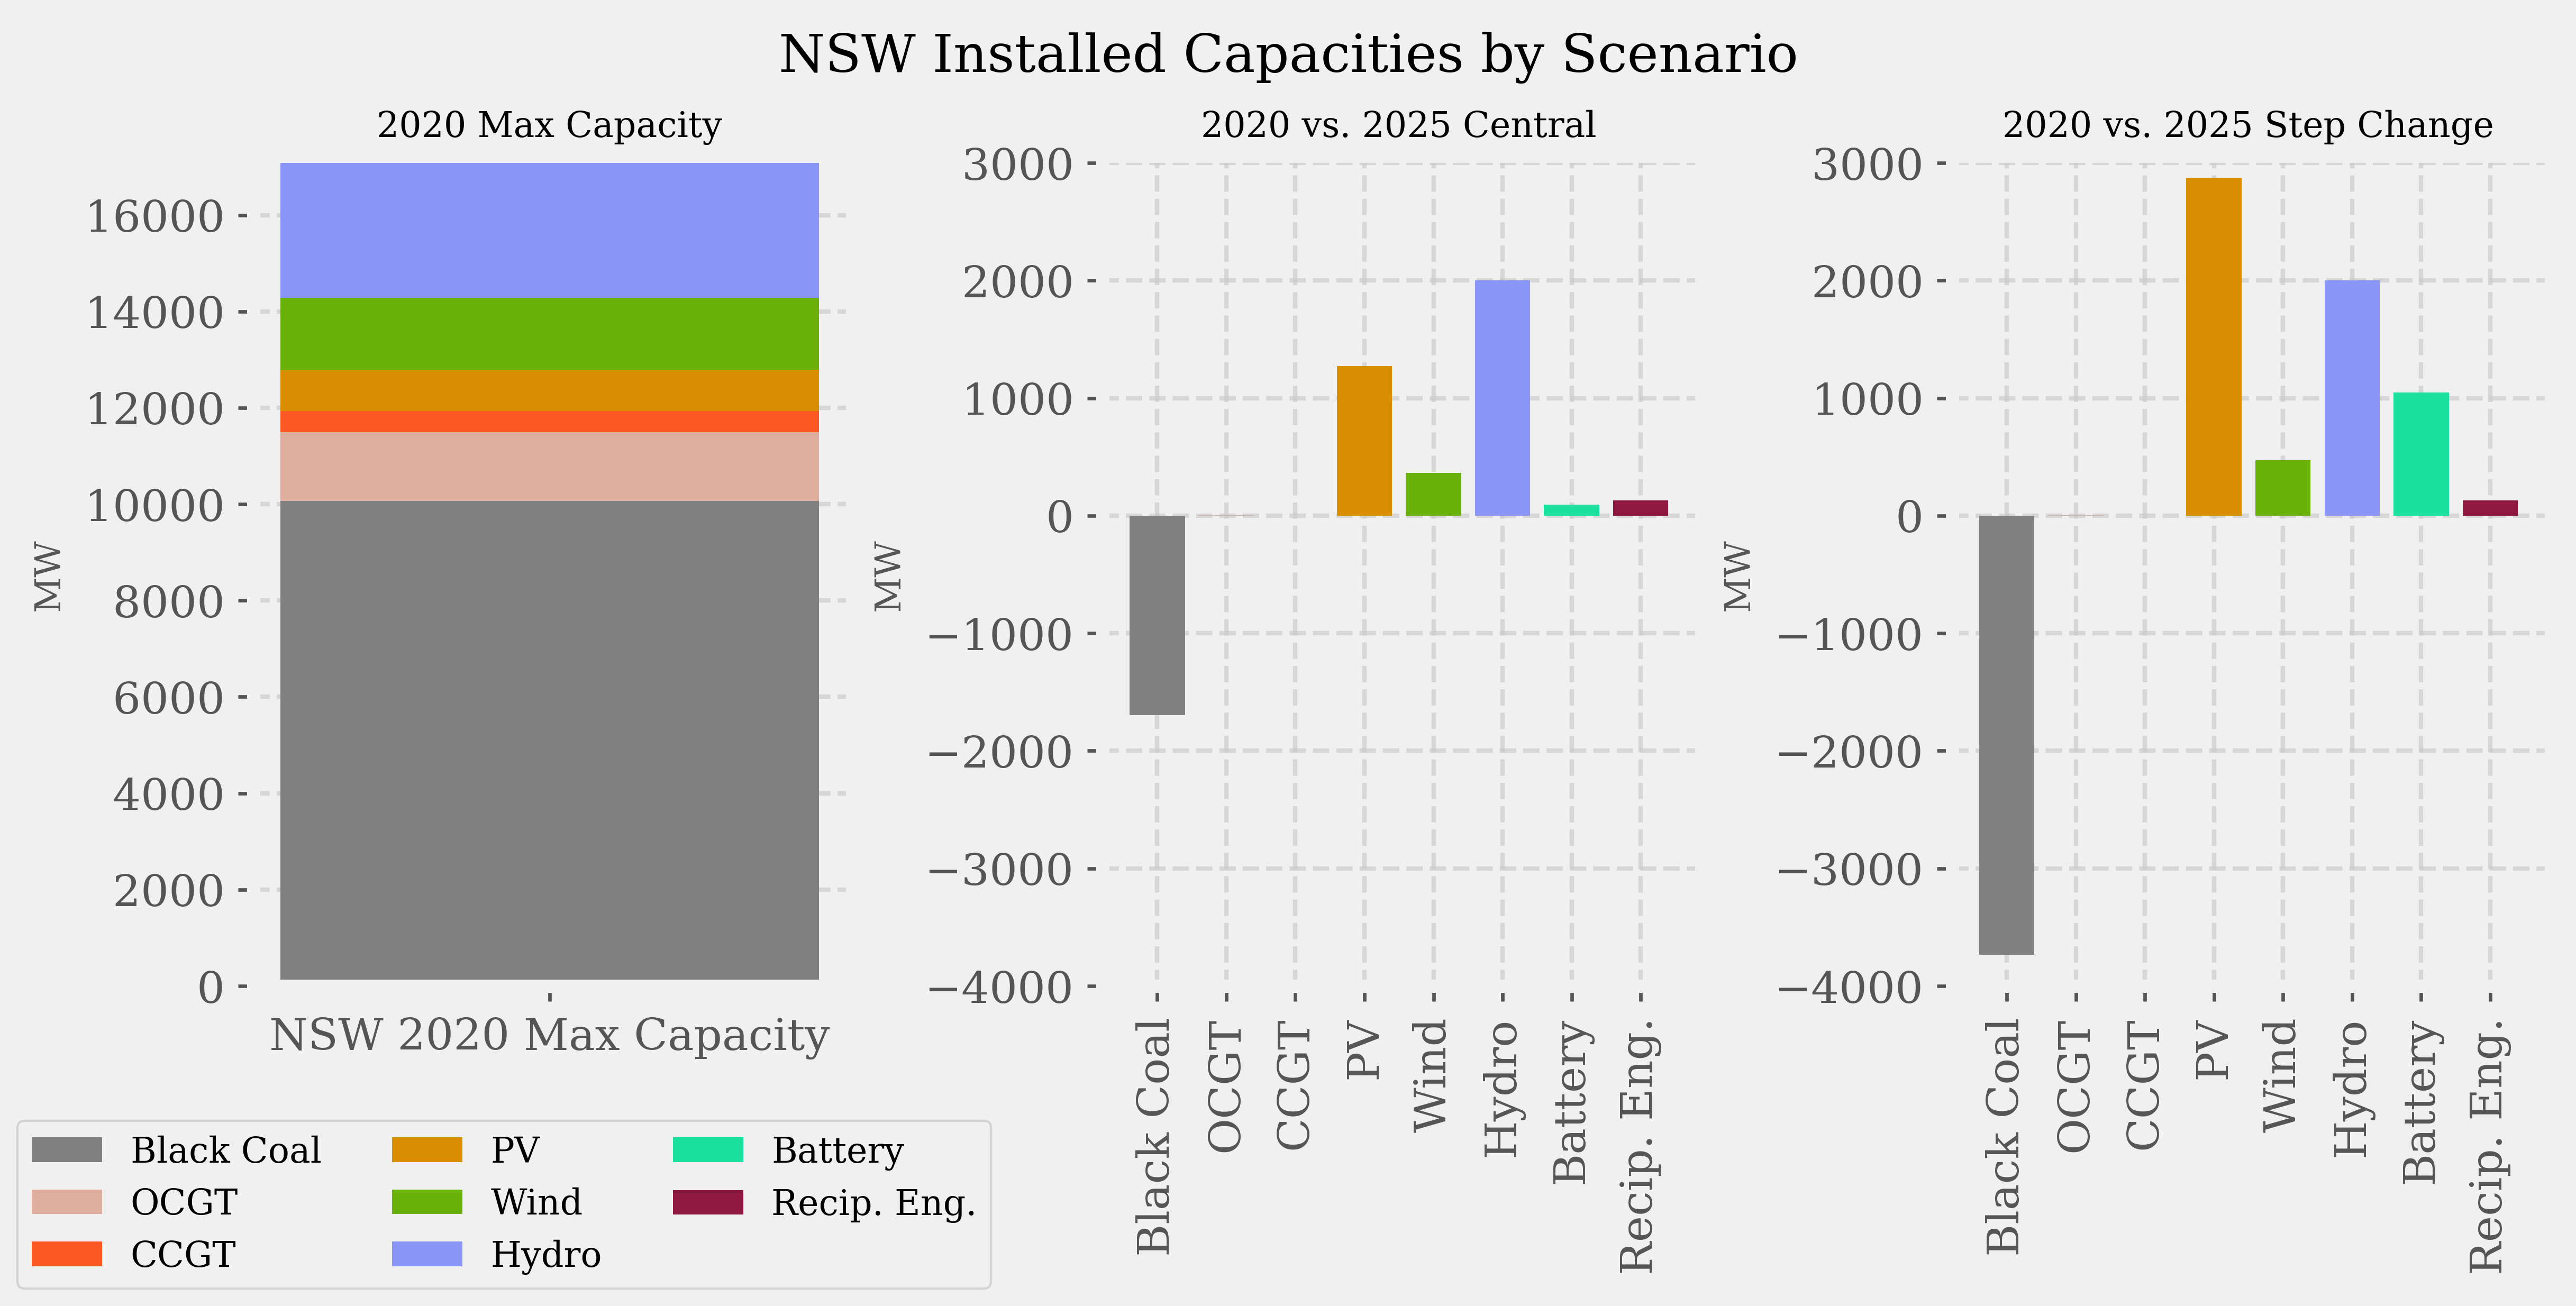
\includegraphics{source/figures/nsw_capacities.png}\label{fig:nsw_capacities}}

\subfloat[]{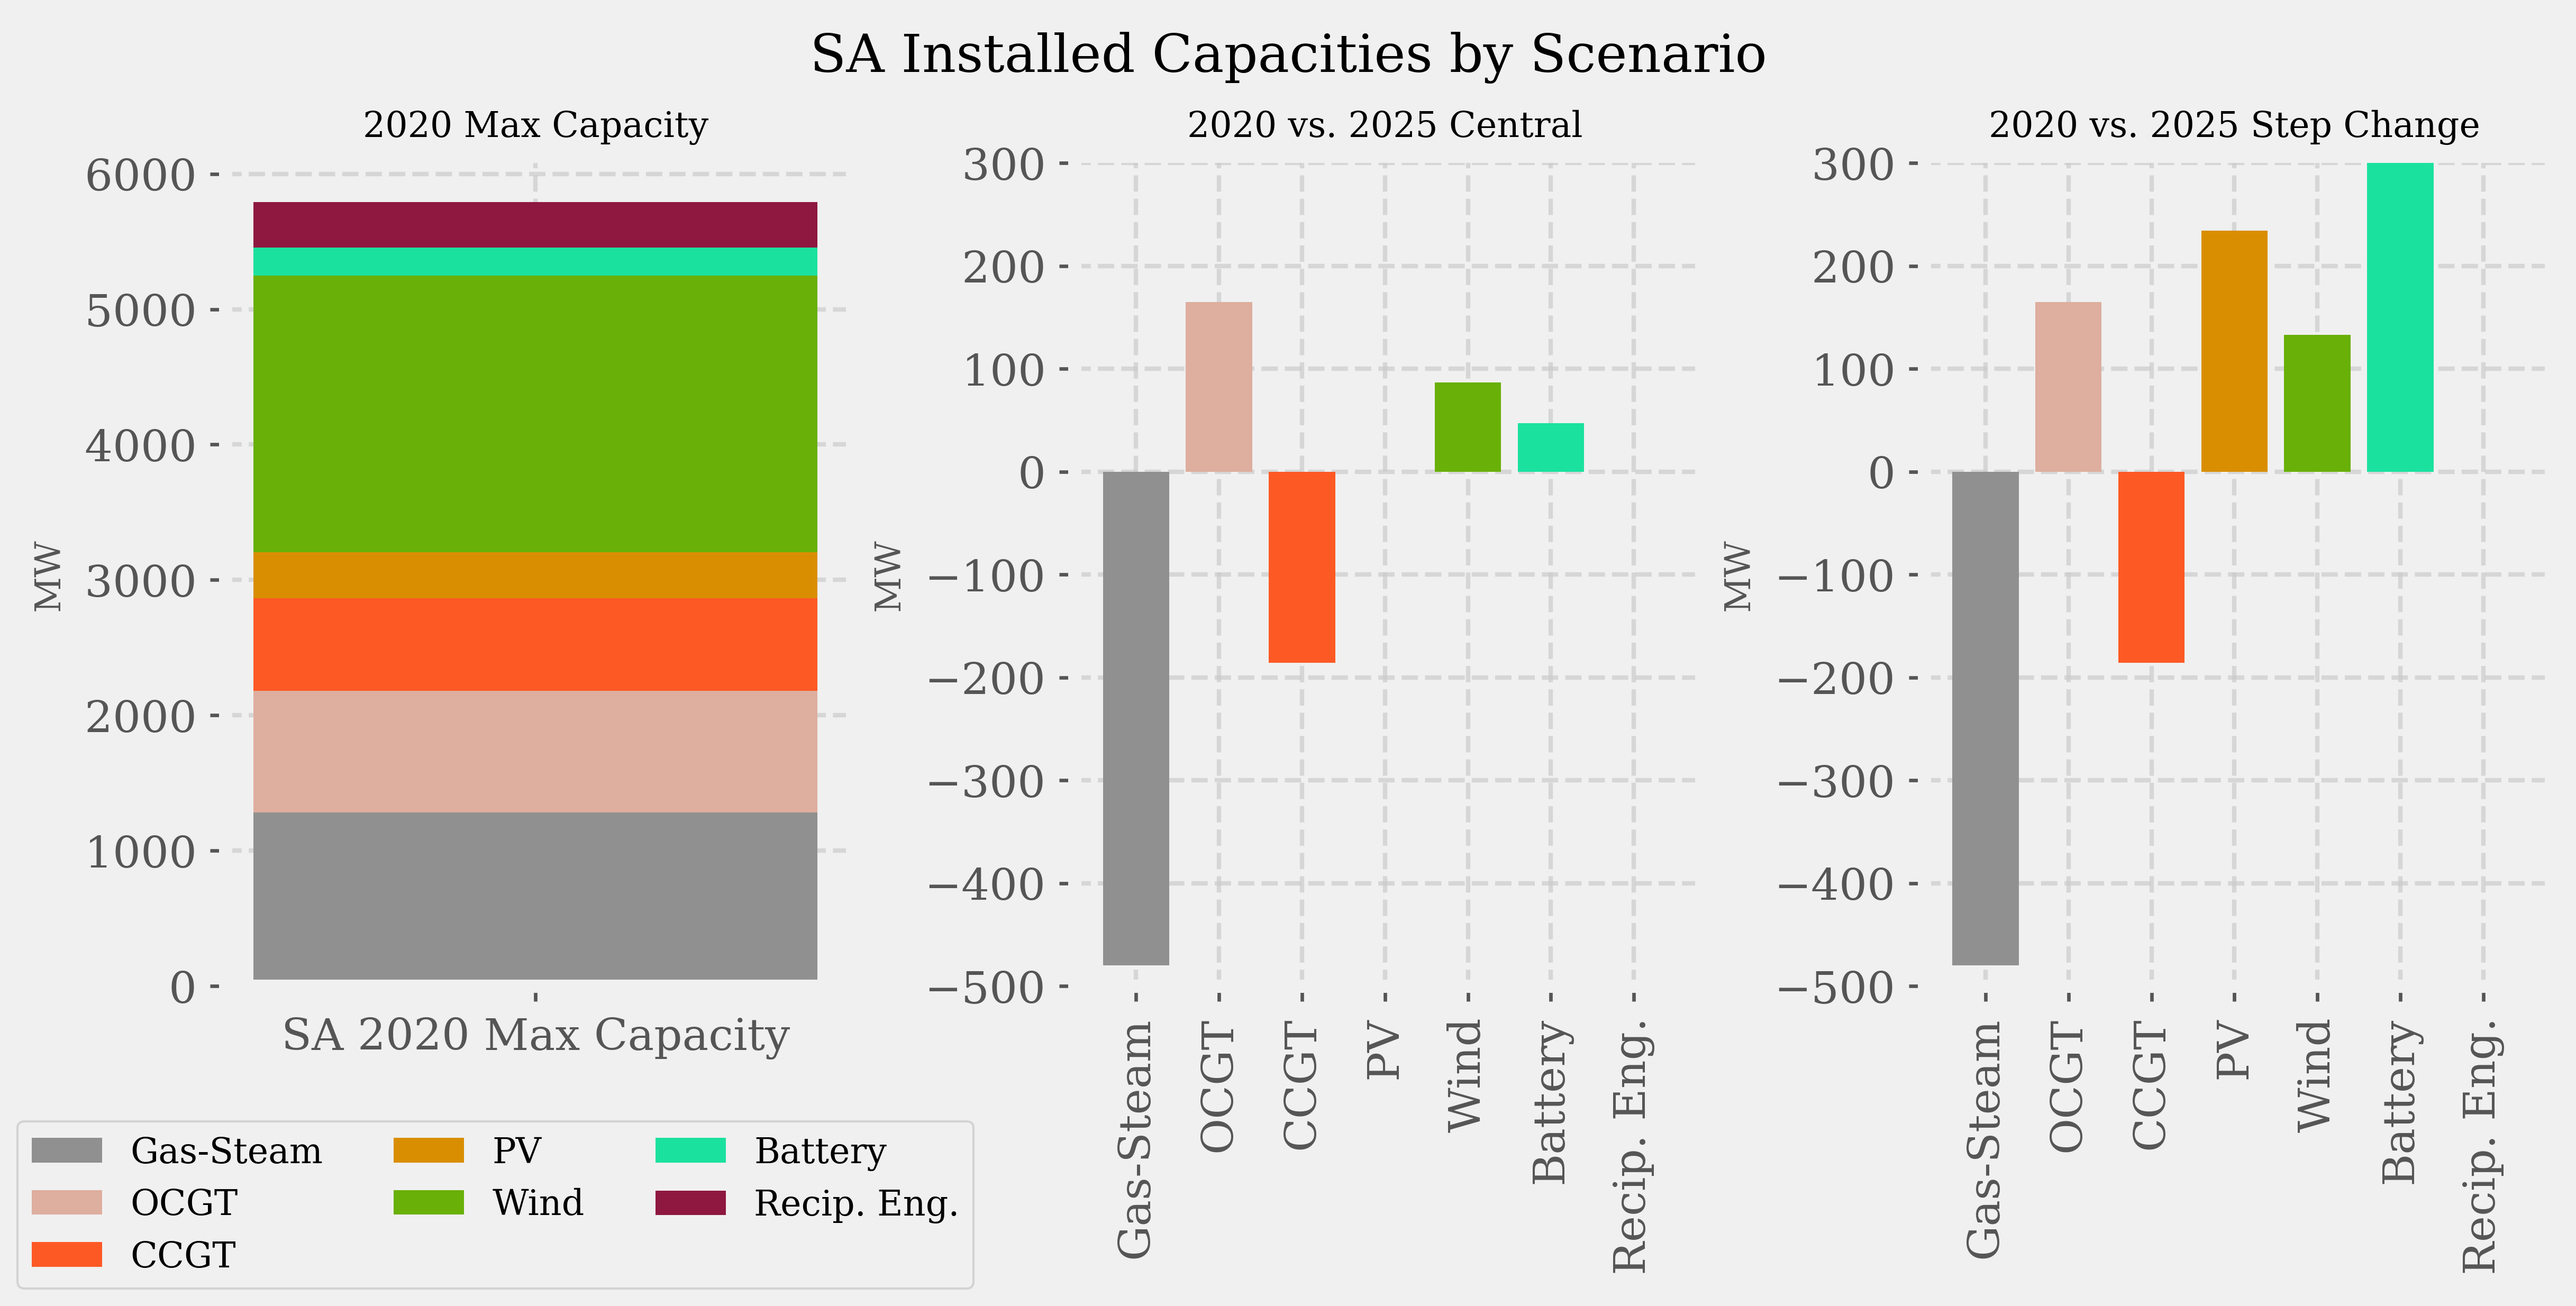
\includegraphics{source/figures/sa_capacities.png}\label{fig:sa_capacities}}

\caption[Capacity mix in NSW and SA in 2020 and the two 2025 scenarios]{Capacity mix in NSW (a) and SA (b) in
2020, and additional deployments and retirements in 2025 Central and
2025 Step Change. 2020 resource mixes were adapted from AEMO's 2020
Inputs and Assumptions workbook
(\protect\hyperlink{ref-australianenergymarketoperator2020InputsAssumptions2020}{Australian
Energy Market Operator, 2020n}). 2025 scenario resource mixes were
aligned with their namesake ISP scenarios
(\protect\hyperlink{ref-australianenergymarketoperator2020ISPGeneration2020}{Australian
Energy Market Operator, 2020m}) and include committed generation
(projects that are highly likely to proceed as they have acquired land,
secured financing, set a firm construction commencement date and either
finalised contracts for components or been granted planning approval)
(\protect\hyperlink{ref-australianenergymarketoperatorGenerationInformation2022}{Australian
Energy Market Operator, 2022b}).}

\label{fig:capacities}

\end{pandoccrossrefsubfigures}

\hypertarget{sec:reserves-method}{%
\section{Methodology}\label{sec:reserves-method}}

For each region and scenario, the available reserves and footroom in the
system were calculated from the results of a year-long time-sequential
market simulation implemented in the commercial electricity market
modelling tool PLEXOS
(\protect\hyperlink{ref-energyexemplarPLEXOSEnergyMarket2021}{Energy
Exemplar, 2021}). The PLEXOS market simulation consisted of a PASA phase
to model maintenance and forced outages for conventional generation
across the year, a Medium Term Schedule phase in NSW to schedule hydro
generation according to monthly energy constraints, and a Short Term
Schedule phase that carries out unit commitment and economic dispatch
(UC-ED) at 5-minute resolution in daily steps\footnote{A 12 hour
  look-ahead was used in the SA model to avoid ``end-of-horizon
  effects''
  (\protect\hyperlink{ref-barrowsIEEEReliabilityTest2020}{Barrows et
  al., 2020}), such as end-of-day decommitment of gas-fired generation.}.

Each existing coal-fired (NSW) and Gas-Steam (SA) unit was explicitly
modelled to accurately capture the consequences of partial and full
outages of large capacity units. For other resource types, the
operational constraints and attributes of individual units were averaged
and applied across all units of a resource type. This enabled clustered
UC-ED and thus reduced the computational burden of the Short Term
Schedule phase
(\protect\hyperlink{ref-palmintierHeterogeneousUnitClustering2014}{Palmintier
and Webster, 2014}). For baseload conventional generation and gas
turbines, ramp rates in each direction were separated into a
\emph{market} ramp rate, which was used in the PLEXOS market simulation,
and an \emph{upper} ramp rate, which was used to calculate available
reserves/footroom (Section~\ref{sec:reserves-conventionalcalc}). A lower
magnitude ramp rate in the market simulation (\emph{market}) reflects
participants' preferences to reduce cycling wear-and-tear due to
demanding ramping during typical operation (especially for ageing
assets) (\protect\hyperlink{ref-kumarPowerPlantCycling2012}{Kumar et
al., 2012}), whilst using a higher magnitude ramp rate to calculate a
resource's available reserves and footroom (\emph{upper}) ensures that
the total available flexibility of a resource can be utilised if needed
in a system emergency.

Both NSW and SA were modelled assuming a copper-plate network with no
interconnection to other regions (i.e.~single bus with no network
constraints). The Short Term Schedule mixed-integer linear program was
solved using the CPLEX Optimizer
(\protect\hyperlink{ref-ibmCPLEXOptimizer2021}{IBM, 2021}) with a
relative mixed-integer program gap tolerance of 0.07\%. The generation
and synchronisation status of each resource was obtained from the
solution and used to calculate the available reserves and footroom for
each 5-minute interval using the equations outlined in
Section~\ref{sec:reserves-modeloverview}. A process flow diagram of the
study methodology is shown in Figure~\ref{fig:method_diagram}.

In Appendix A, we outline our sources for key input data and assumptions
(top row of Figure~\ref{fig:method_diagram}) and provide further details
regarding how these data were used in the market simulation and/or the
calculation of available reserves and footroom.

\begin{figure}
\hypertarget{fig:method_diagram}{%
\centering
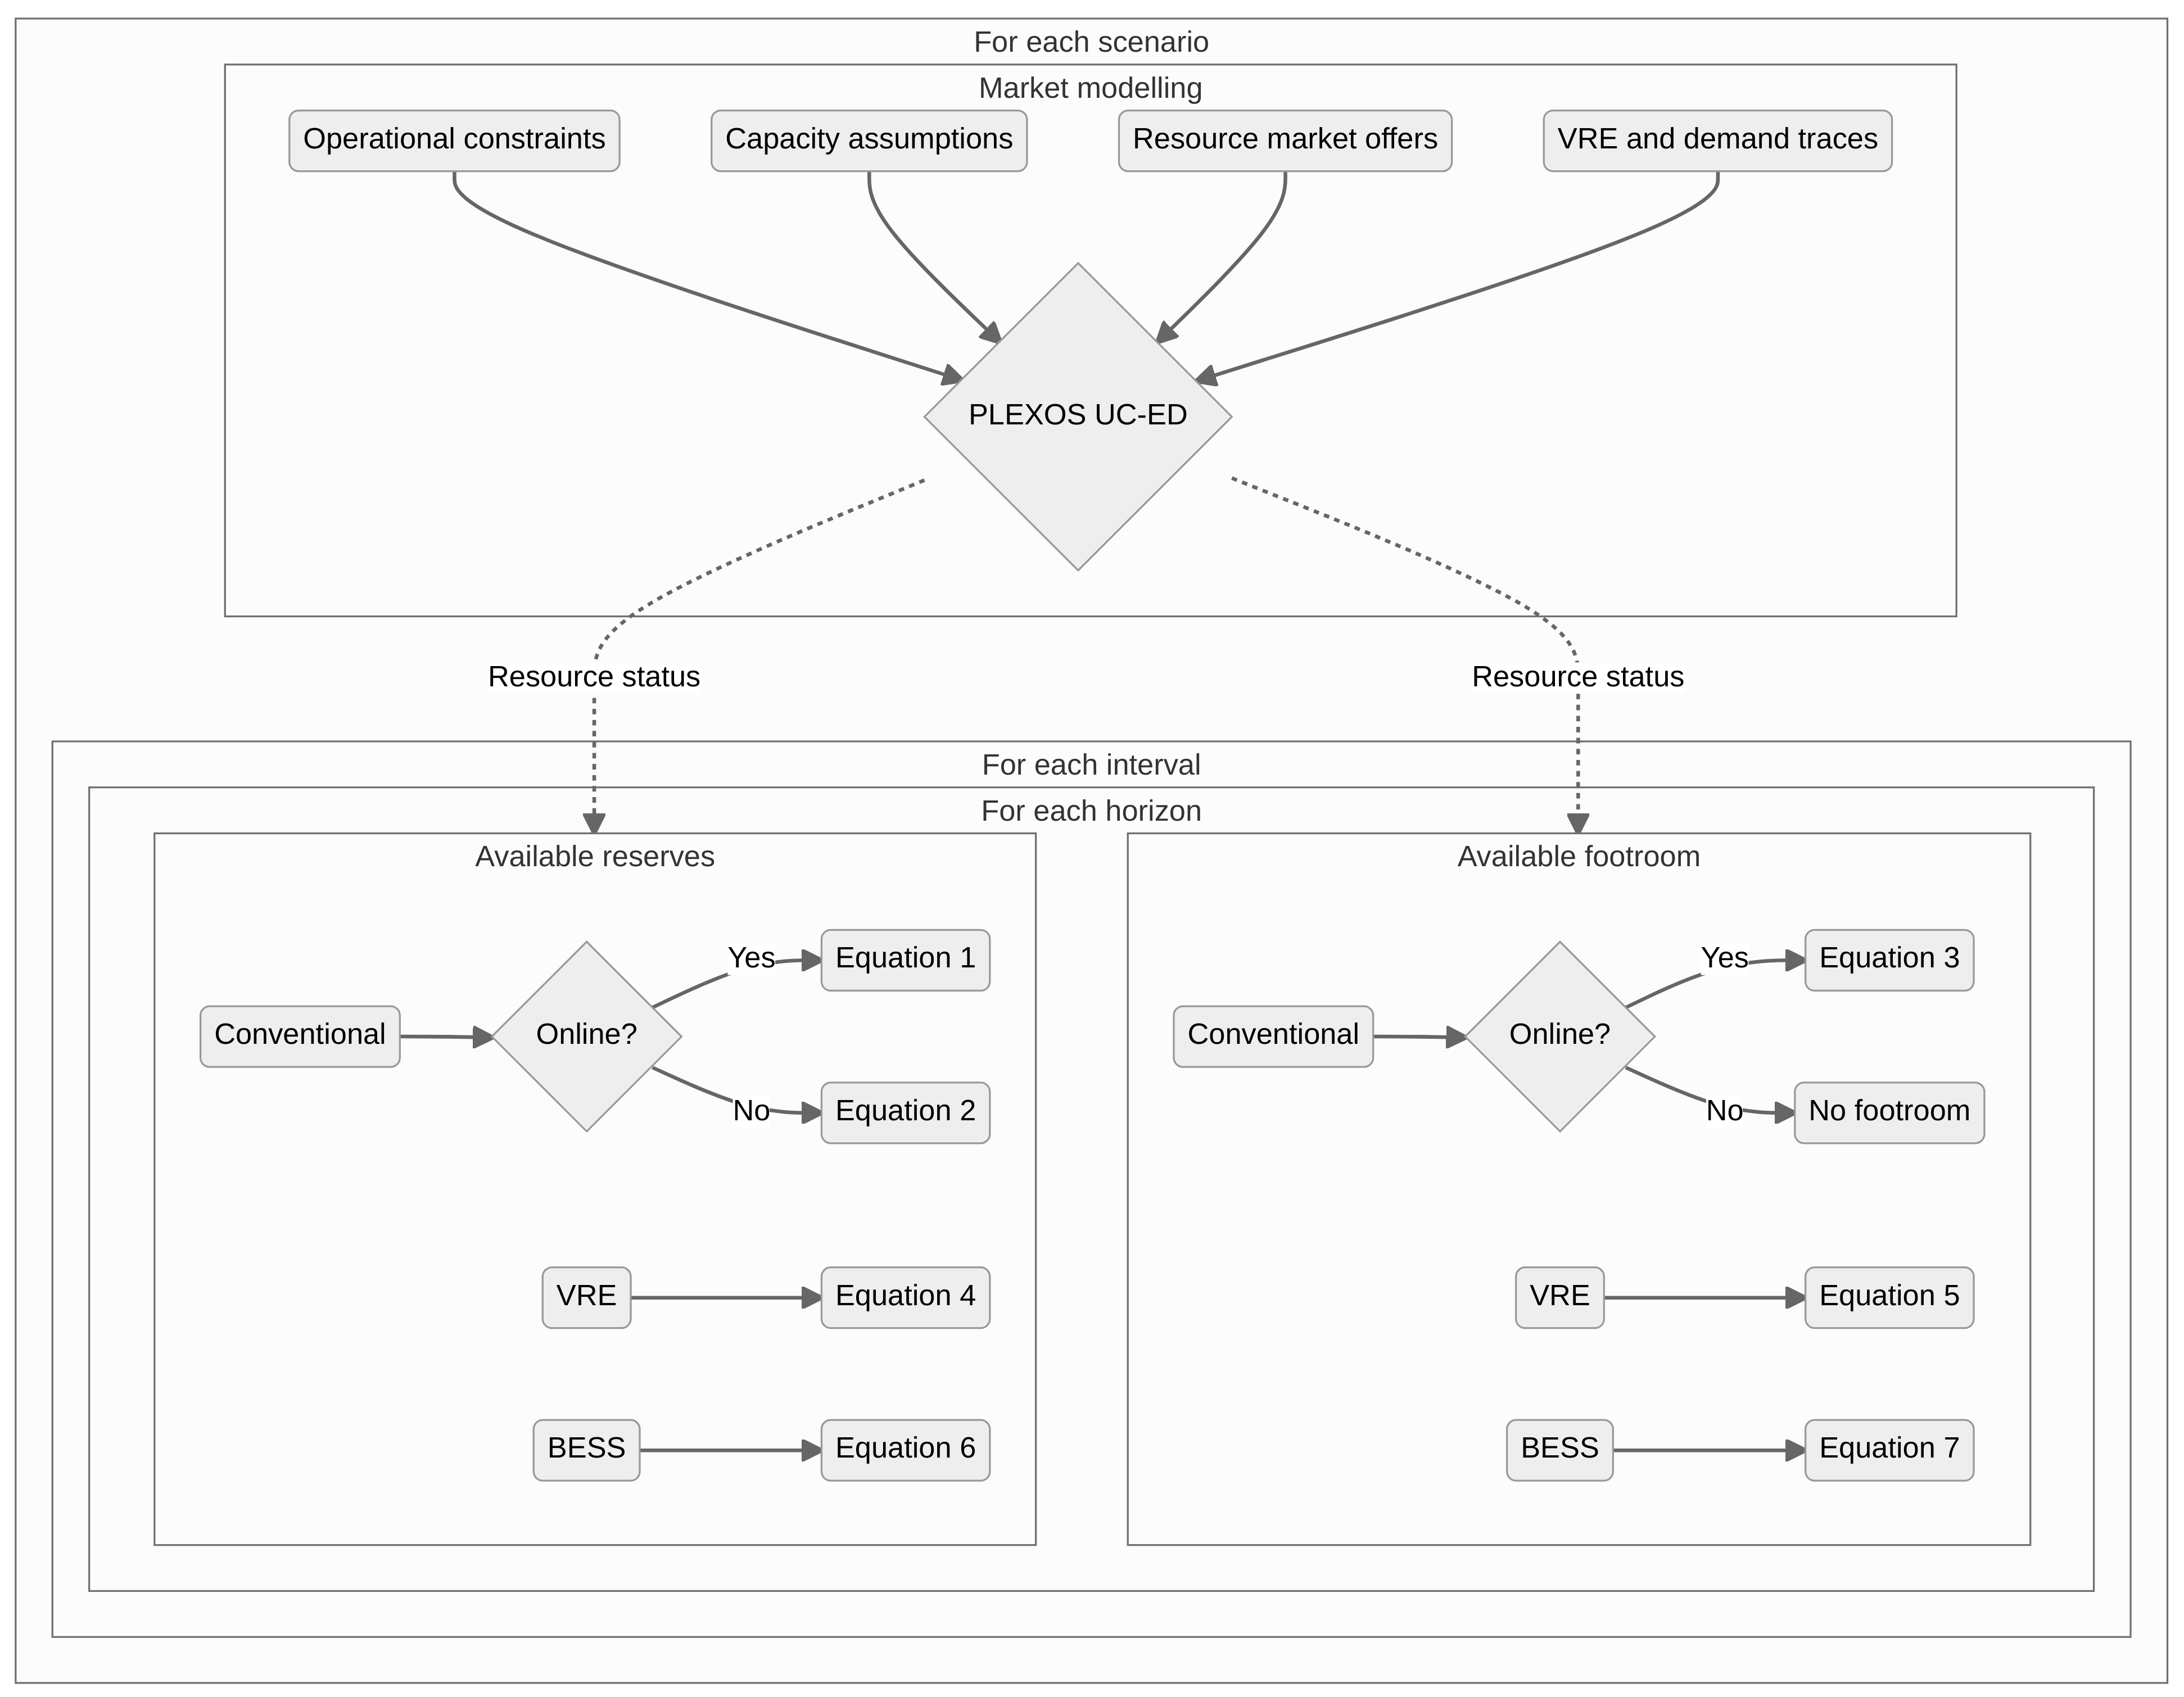
\includegraphics[width=1\textwidth,height=\textheight]{source/figures/modelling_diagram.png}
\caption[Process flow diagram for modelling available reserves and
footroom for each scenario]{Process flow for modelling available
reserves and footroom for each scenario in this case
study.}\label{fig:method_diagram}
}
\end{figure}

\hypertarget{limitations-1}{%
\subsection{Limitations}\label{limitations-1}}

There are two important caveats to this study. The first is that this
study models each region in isolation -- that is, resources in other NEM
regions can neither assist in meeting demand nor provide available
reserves or footroom through cross-regional interconnectors. During
typical operating conditions, it is likely that any headroom/footroom on
interconnectors would mean that a greater quantity of reserves/footroom
are available to a region, albeit at different horizons due to modified
dispatch patterns. For example, the inclusion of interconnectors in the
SA model between SA and VIC and SA and NSW\footnote{At the time of
  writing, the interconnector between SA and NSW is under construction
  and due to commence operation in 2025/2026
  (\protect\hyperlink{ref-electranettransgridProjectEnergyConnect}{ElectraNet,
  Transgrid, n.d.}).} may increase the total available reserves/footroom
in SA at the cost of a decrease in the reserves/footroom available
within shorter horizons. This could arise from local mid-merit gas
generators remaining offline in favour of inflexible but cheaper
coal-fired generation in NSW and VIC.

However, modelling available reserves and footroom for isolated regions
may provide a closer approximation to reality when balancing flexibility
is scarce in a region. Under these circumstances, it is likely that
interconnector flows will already be close to their limits. This will
reduce or altogether prevent the available reserves/footroom provision
from resources in neighbouring regions. Moreover, large interconnector
flows may be prevented if there is a credible risk of regional
separation (loss of synchronism between market regions due to
interconnector circuit faults --- a particular risk in the NEM due to
limited interconnection between market regions); at present, AEMO
co-optimises interconnector flow with regional FCAS procurement
(\protect\hyperlink{ref-australianenergymarketoperatorConstraintFormulationGuidelines2010}{Australian
Energy Market Operator, 2010}). An additional consideration is that if
an operating reserve product is implemented to improve the NEM's
resilience to supply-demand shocks, regional procurement requirements
may also limit the available reserves/footroom that can be procured over
an interconnector. As such, the modelling of isolated regions may
approximate actual operation when reserves/footroom are scarce and thus
most valuable to the system.

The second caveat is that this study does not explicitly model FCAS
procurement. If headroom or footroom reserved for FCAS is unable to also
provide available reserves or footroom\footnote{Exclusive headroom
  procurement for an operating reserve service (i.e.~inability to offer
  the same headroom in FCAS markets) is currently being considered
  (\protect\hyperlink{ref-energysecurityboardPost2025Market2021}{Energy
  Security Board, 2021}).}, then modelling FCAS markets would reduce the
reserves and footroom that are available within horizons less than or
equal to 5 minutes. However, the actual headroom/footroom reduction
would depend upon the following factors:

\begin{itemize}
\tightlist
\item
  Whether regional FCAS procurement constraints bind for the modelled
  region. If they do not, multi-regional or NEM-wide FCAS requirements
  can be satisfied by procuring FCAS in other market regions.
\item
  The degree to which headroom/footroom is ``re-offered'' across
  sequential FCAS markets. For example, a single resource enabled for 10
  MW across the three raise contingency FCAS markets would withdraw less
  system headroom than three resources enabled for 10 MW each for a
  particular FCAS market.
\item
  Headroom that is offered into the 6 second and 60 second raise
  contingency FCAS market may not reflect sustained power provision. For
  example, frequency response from a steam-powered turbine may draw on
  steam stored in a boiler; a sustained response would require a longer
  timeframe due to slower boiler dynamics.
\end{itemize}

\hypertarget{sec:reserves-results}{%
\subsection{Results and discussion}\label{sec:reserves-results}}

\hypertarget{synthetic-daily-profiles}{%
\subsubsection{Synthetic daily
profiles}\label{synthetic-daily-profiles}}

\emph{Synthetic daily profiles} (SDPs) were developed to quantify the
time-varying spectrum of available reserves and footroom for each
scenario. For a given horizon, the SDP value at a particular time is an
aggregate value (mean or a specific percentile) calculated from the
reserves/footroom available within that horizon at the end of that
dispatch interval across all days in the simulated year. In other words,
values from across the year for a given time of day are aggregated, and
these are then ``stitched'' together to form a ``synthetic day'' curve
for a particular horizon. Two aggregate values were calculated for each
horizon curve:

\begin{enumerate}
\def\labelenumi{\arabic{enumi}.}
\tightlist
\item
  The mean. This provides a picture of the average or ``typical''
  availability of reserves and footroom at different times of the day
  for a particular scenario year; and
\item
  The bottom 1\% (i.e.~1\textsuperscript{st} percentile or 1-in-100 day
  lowest). This measure better reflects the availability of reserves and
  footroom when they are scarce and thus when they are most
  needed\footnote{More extreme percentiles (i.e.~\textless{} 1\%) could
    better reflect the tight reliability standards adopted in many power
    systems - e.g.~the NEM standard of a maximum expected unserved
    energy of 0.002\% of the total energy demand of a NEM region in an
    Australian financial year
    (\protect\hyperlink{ref-australianenergymarketcommissionreliabilitypanel2022ReviewReliability2022}{Australian
    Energy Market Commission Reliability Panel, 2022}). However, the use
    of extreme percentiles would be more appropriate with a greater
    number of modelled days (i.e.~several years).}.
\end{enumerate}

In addition to an infinite horizon (which corresponds to the maximum
availability), curves were calculated for 1, 5, 15, 30 and 60 minute
horizons. These horizons encompass the start-up times of hydro and
flexible gas generation, and represent the likely timeframes over which
the proposed operating reserve product will be required to respond.

\hypertarget{sec:reserves-reserveSDPs}{%
\subsubsection{Available reserve synthetic
days}\label{sec:reserves-reserveSDPs}}

Mean and bottom 1\% available reserve SDPs were generated for the NSW
scenarios and for the SA scenarios
(Figures~\ref{fig:nswreserves}, \ref{fig:sareserves}). The mean SDPs
across scenarios suggest that, on average, NSW has more than 2 GW and SA
more than 600 MW of reserves available within 5+ minutes. These levels
of reserves:

\begin{enumerate}
\def\labelenumi{\arabic{enumi}.}
\tightlist
\item
  Correspond to approximately 15\% and 20\% of peak demand in 2020 in
  NSW and SA, respectively. These 5+ minute ``reserve margins'' (i.e.~5+
  minute reserves as a percentage of peak demand) are comparable to
  lower-end reserve margins anticipated for the summer of 2022 in North
  American jurisdictions
  (\protect\hyperlink{ref-northamericanelectricreliabilitycorporation2022SummerReliability2022}{North
  American Electric Reliability Corporation, 2022}).
\item
  Exceed the highest N-1 contingency in 2020 (i.e.~highest LOR2 trigger
  level declared in the last run of Pre-Dispatch PASA prior to delivery
  --- see Section~\ref{sec:reserves-ahead_soint}) by approximately 225\%
  in NSW and 170\% in SA
  (\protect\hyperlink{ref-prakashNEMSEER2022}{Prakash, 2022}).
\end{enumerate}

Furthermore, with additional BESS and flexible gas resources expected to
be deployed, the mean 5+ minute reserve margins of both regions are
higher for most parts of the day in the 2025 Step Change scenario.
Though the market simulation relied on perfect foresight (additional
uncertainty may reduce reserve margins), these results suggest that
reasonable quantities of reserves are available in each region within a
5+ minute horizon.

\begin{figure}
\hypertarget{fig:nswreserves}{%
\centering
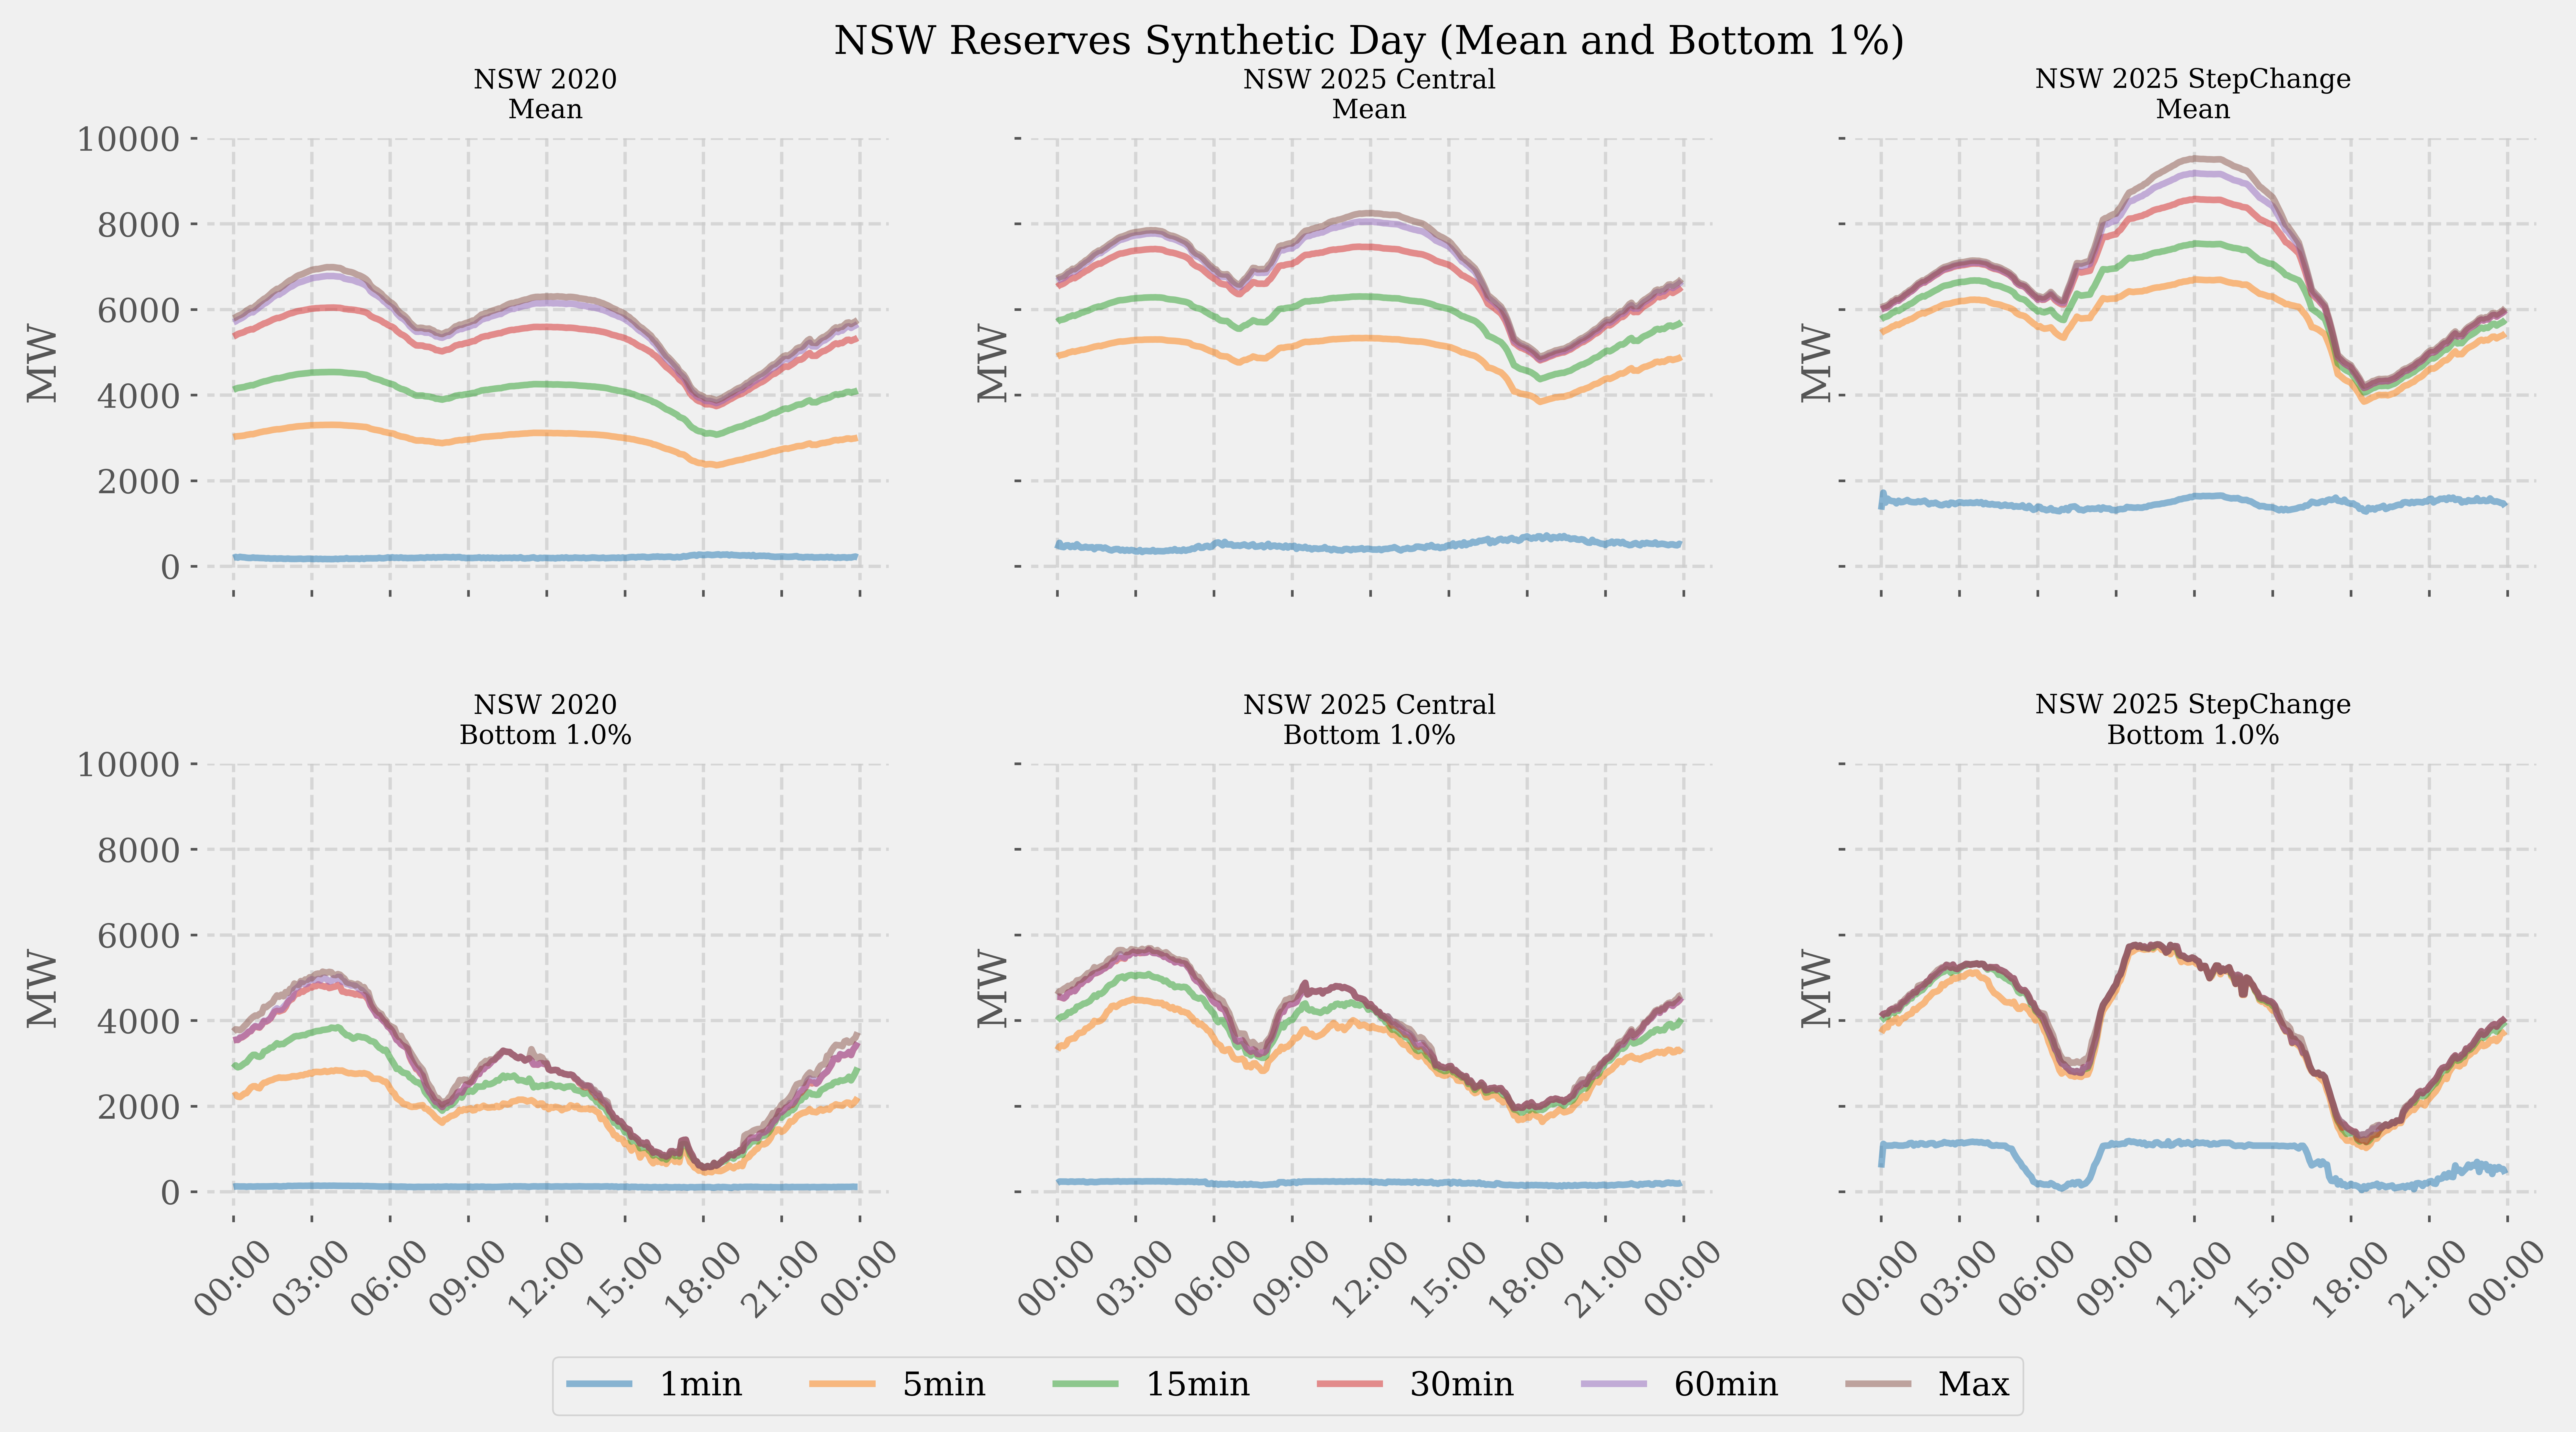
\includegraphics[width=1\textwidth,height=\textheight]{./source/figures/NSW_reserves_all_profiles_by_di.png}
\caption[NSW available reserves SDPs]{Mean (top row) and bottom 1\%
(bottom row) SDPs for available reserves in NSW in 2020 (leftmost
column) and the two 2025 scenarios (rightmost
columns).}\label{fig:nswreserves}
}
\end{figure}

\begin{figure}
\hypertarget{fig:sareserves}{%
\centering
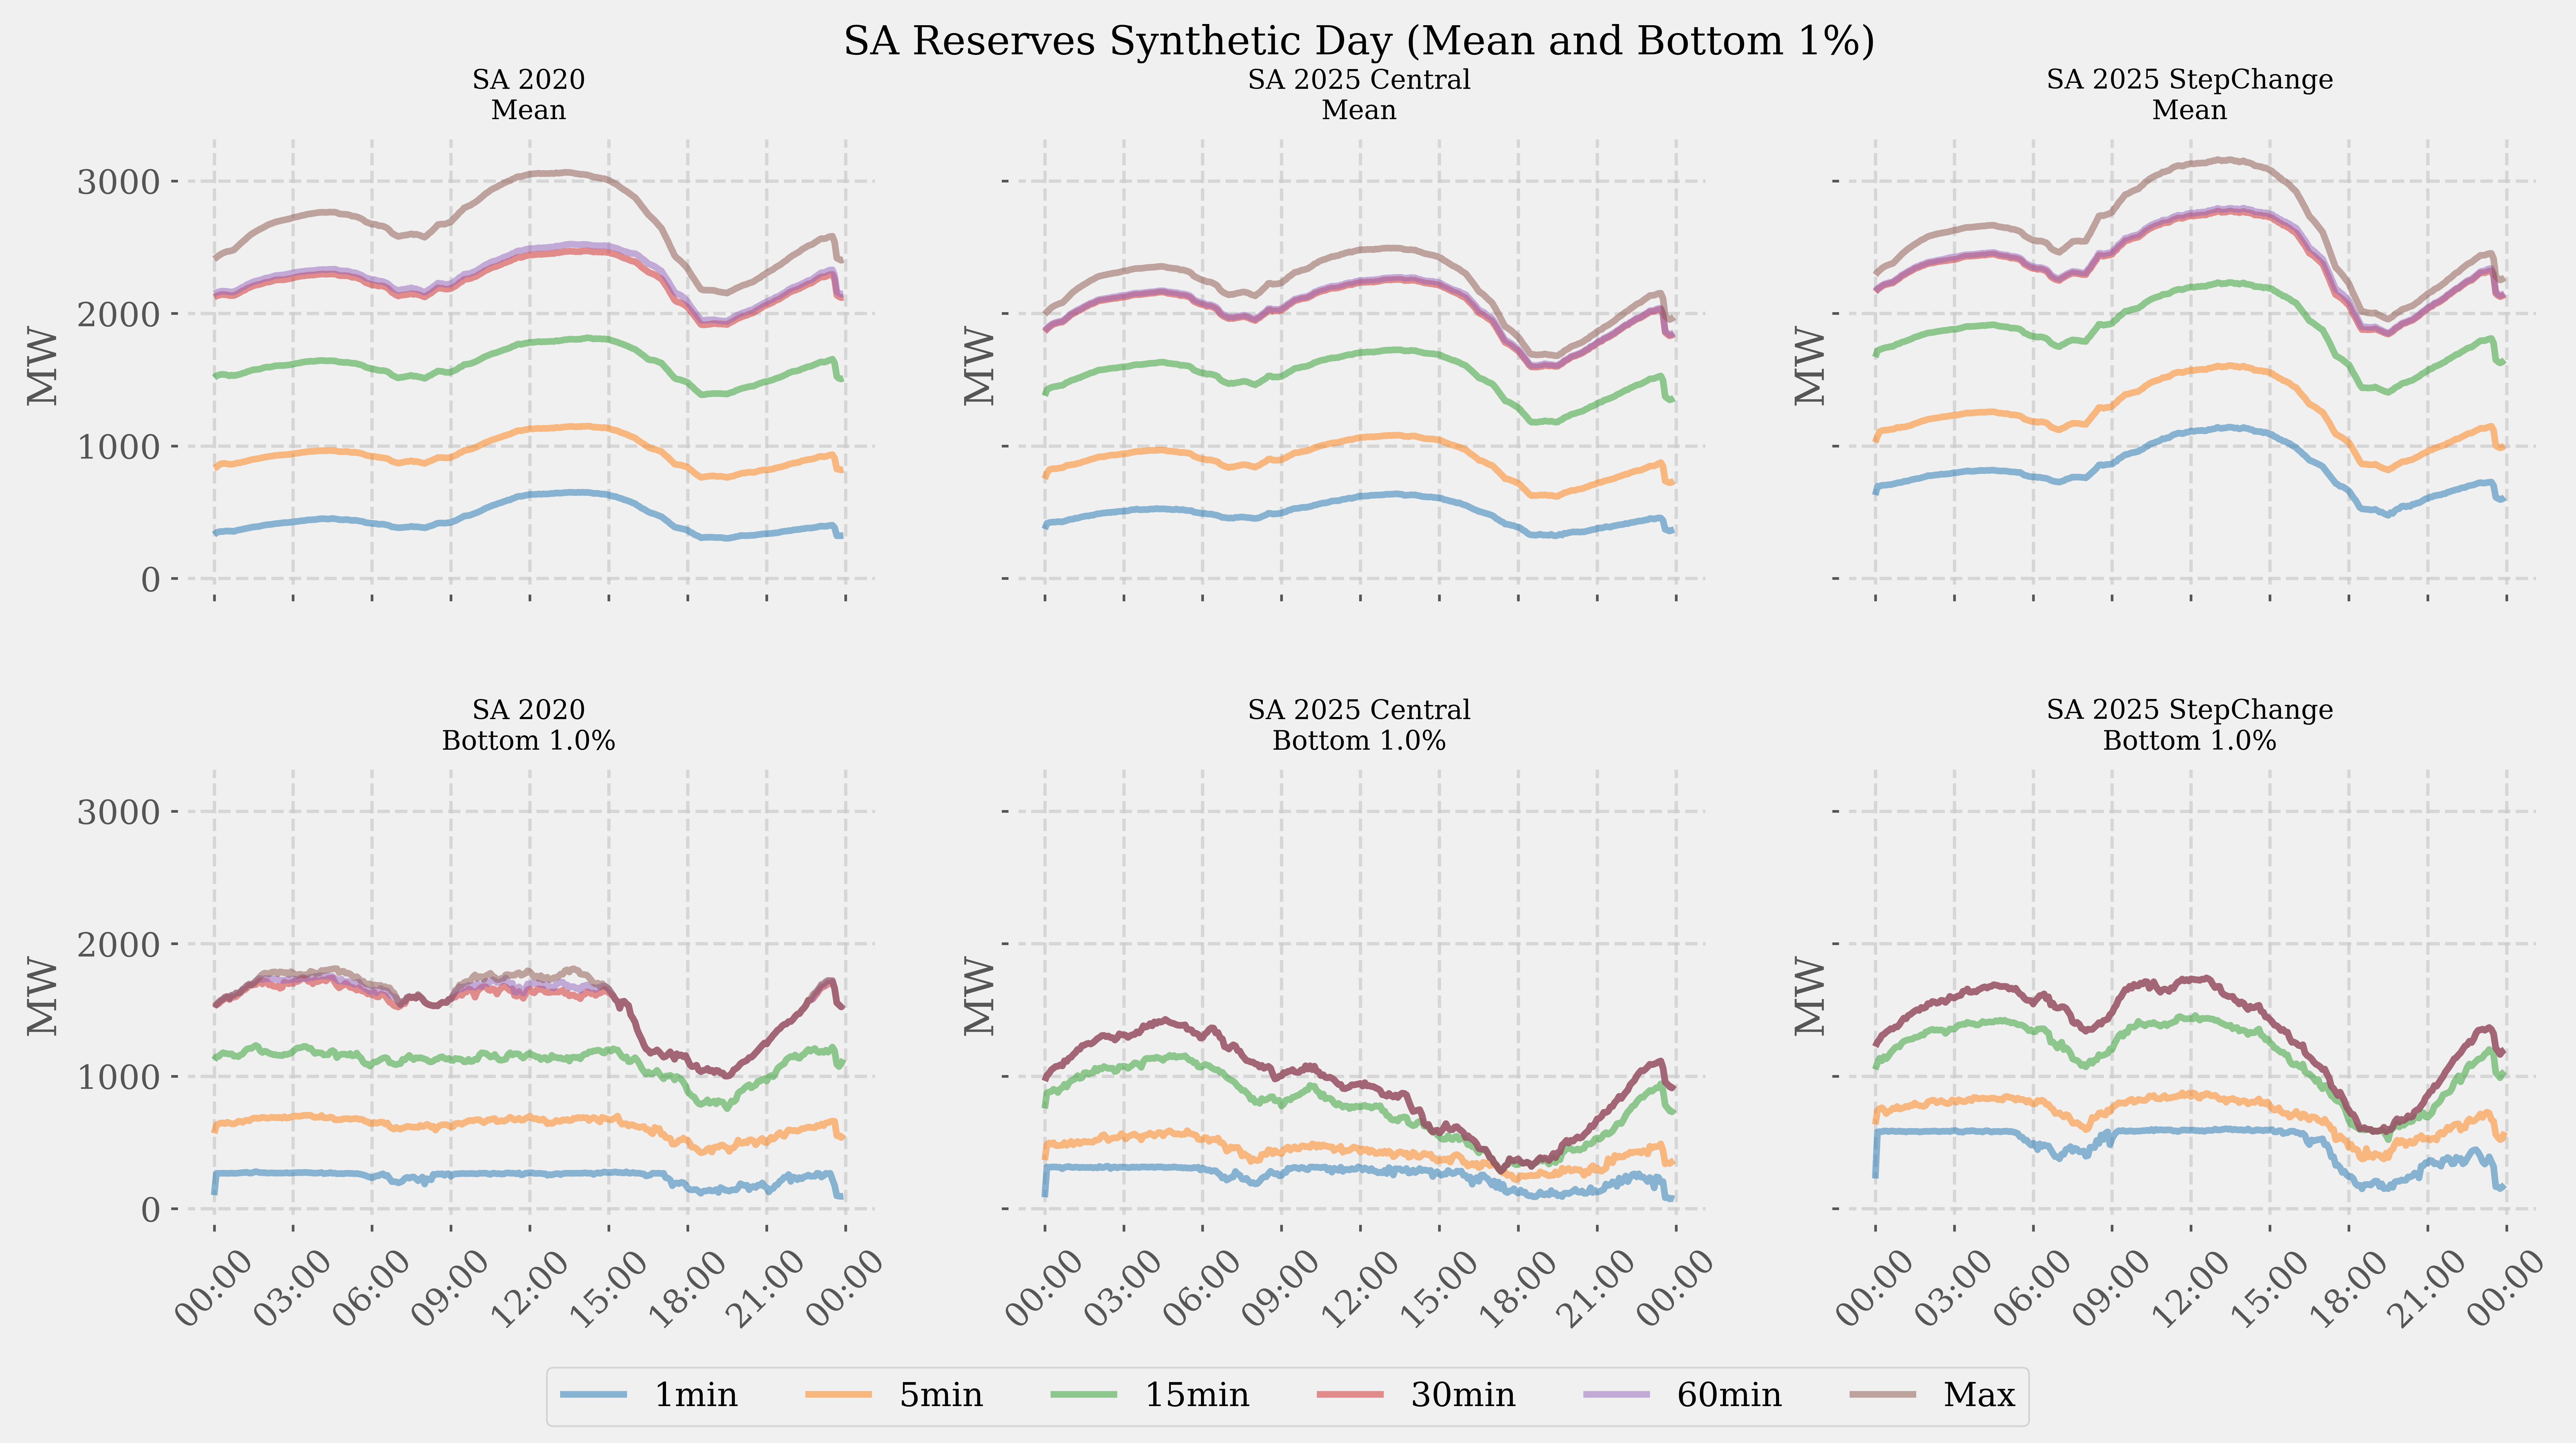
\includegraphics[width=1\textwidth,height=\textheight]{./source/figures/SA_reserves_all_profiles_by_di.png}
\caption[SA available reserves SDPs]{Mean (top row) and bottom 1\%
(bottom row) SDPs for available reserves in SA in 2020 (leftmost column)
and the two 2025 scenarios (rightmost columns).}\label{fig:sareserves}
}
\end{figure}

Across scenarios, the following trends are apparent in the SDPs:

\begin{enumerate}
\def\labelenumi{\arabic{enumi}.}
\tightlist
\item
  From 2020 to the 2025 Step Change scenario, a midday peak in the mean
  available reserves SDPs becomes more pronounced. This can be
  attributed to the increasing displacement of conventional generation
  by lower-cost utility-scale solar PV in dispatch (an outcome observed
  by Hummon et al.
  (\protect\hyperlink{ref-hummonFundamentalDriversCost2013}{2013}) and
  Tanoto et al.
  (\protect\hyperlink{ref-tanotoImpactHighSolar2021}{2021})) and the
  progressive erosion of daytime operational demand due to higher
  penetrations of distributed solar PV. Particularly in SA, curtailed
  VRE and BESS also contribute to this reserve ``surplus''. BESS in
  particular are often charging during such periods of plentiful supply
  and low prices, and thus are able to offer up to double their active
  power rating as reserve (i.e.~by switching from charging to
  discharging).
\item
  As is particularly clear in the bottom 1\% SDPs for the 2025
  scenarios, the availabilities of different reserve horizons tend to
  converge during periods of lower reserves or ``relative scarcity'',
  which include peak demand events in the morning and evening. The
  convergence may be driven by the retirement of baseload conventional
  generation and higher ramping requirements in the 2025 scenarios
  requiring more flexible, mid-merit resources to be online prior to and
  during these periods.
\end{enumerate}

From this analysis, we can also gain an insight into the supply-side
dynamics of a potential operating reserve product market. The first
trend suggests that as energy transition proceeds, a reserve surplus
during the daytime could suppress the price of an operating reserve
product (a dynamic that is further explored by Frew et al.
(\protect\hyperlink{ref-frewCurtailmentParadoxTransition2021}{2021b})).
Moreover, the convergence of availability across horizons during periods
of ``relative scarcity'' suggests that relatively inflexible but cheaper
resources are being preferentially ramped through dispatch at these
times whilst more flexible but expensive resources are left in reserve.
Since the majority of system headroom during these periods appears to be
available within 5 to 15 minutes, operating reserves would likely be
procured from these more flexible resources regardless of whether the
product requires availability within 5 or 30 minutes. As such, concerns
regarding limited providers of a 5-minute horizon product may also apply
to a 30-minute horizon product during periods of relative scarcity
(noting that several resource types in the NEM are already providing
upwards flexibility within 5 minutes in the NEM, as shown in
Figure~\ref{fig:raise_delayed_supply}).

\hypertarget{sec:reserves-footroomSDPs}{%
\subsubsection{Available footroom synthetic
days}\label{sec:reserves-footroomSDPs}}

Two types of SDPs were constructed for available footroom: one for
\emph{firm} footroom and the other for total footroom. The former refers
to potential footroom provision from conventional resources and BESS,
whereas the latter also includes footroom that can be provided by
curtailing VRE. Figures~\ref{fig:nswfirmfoot}, \ref{fig:nswfoot} show
mean and bottom 1\% SDPs across NSW scenarios for firm footroom and
total footroom, respectively. From the bottom 1\% SDPs in
Figure~\ref{fig:nswfirmfoot}, it is clear that firm system footroom can
become very low in NSW in 2025 as remaining baseload conventional
generators are driven to operate closer to their MSLs. However, such
concerns could be alleviated if VRE provide footroom
(Figure~\ref{fig:nswfoot}). A similar result was observed for the SA
region.

\begin{figure}
\hypertarget{fig:nswfirmfoot}{%
\centering
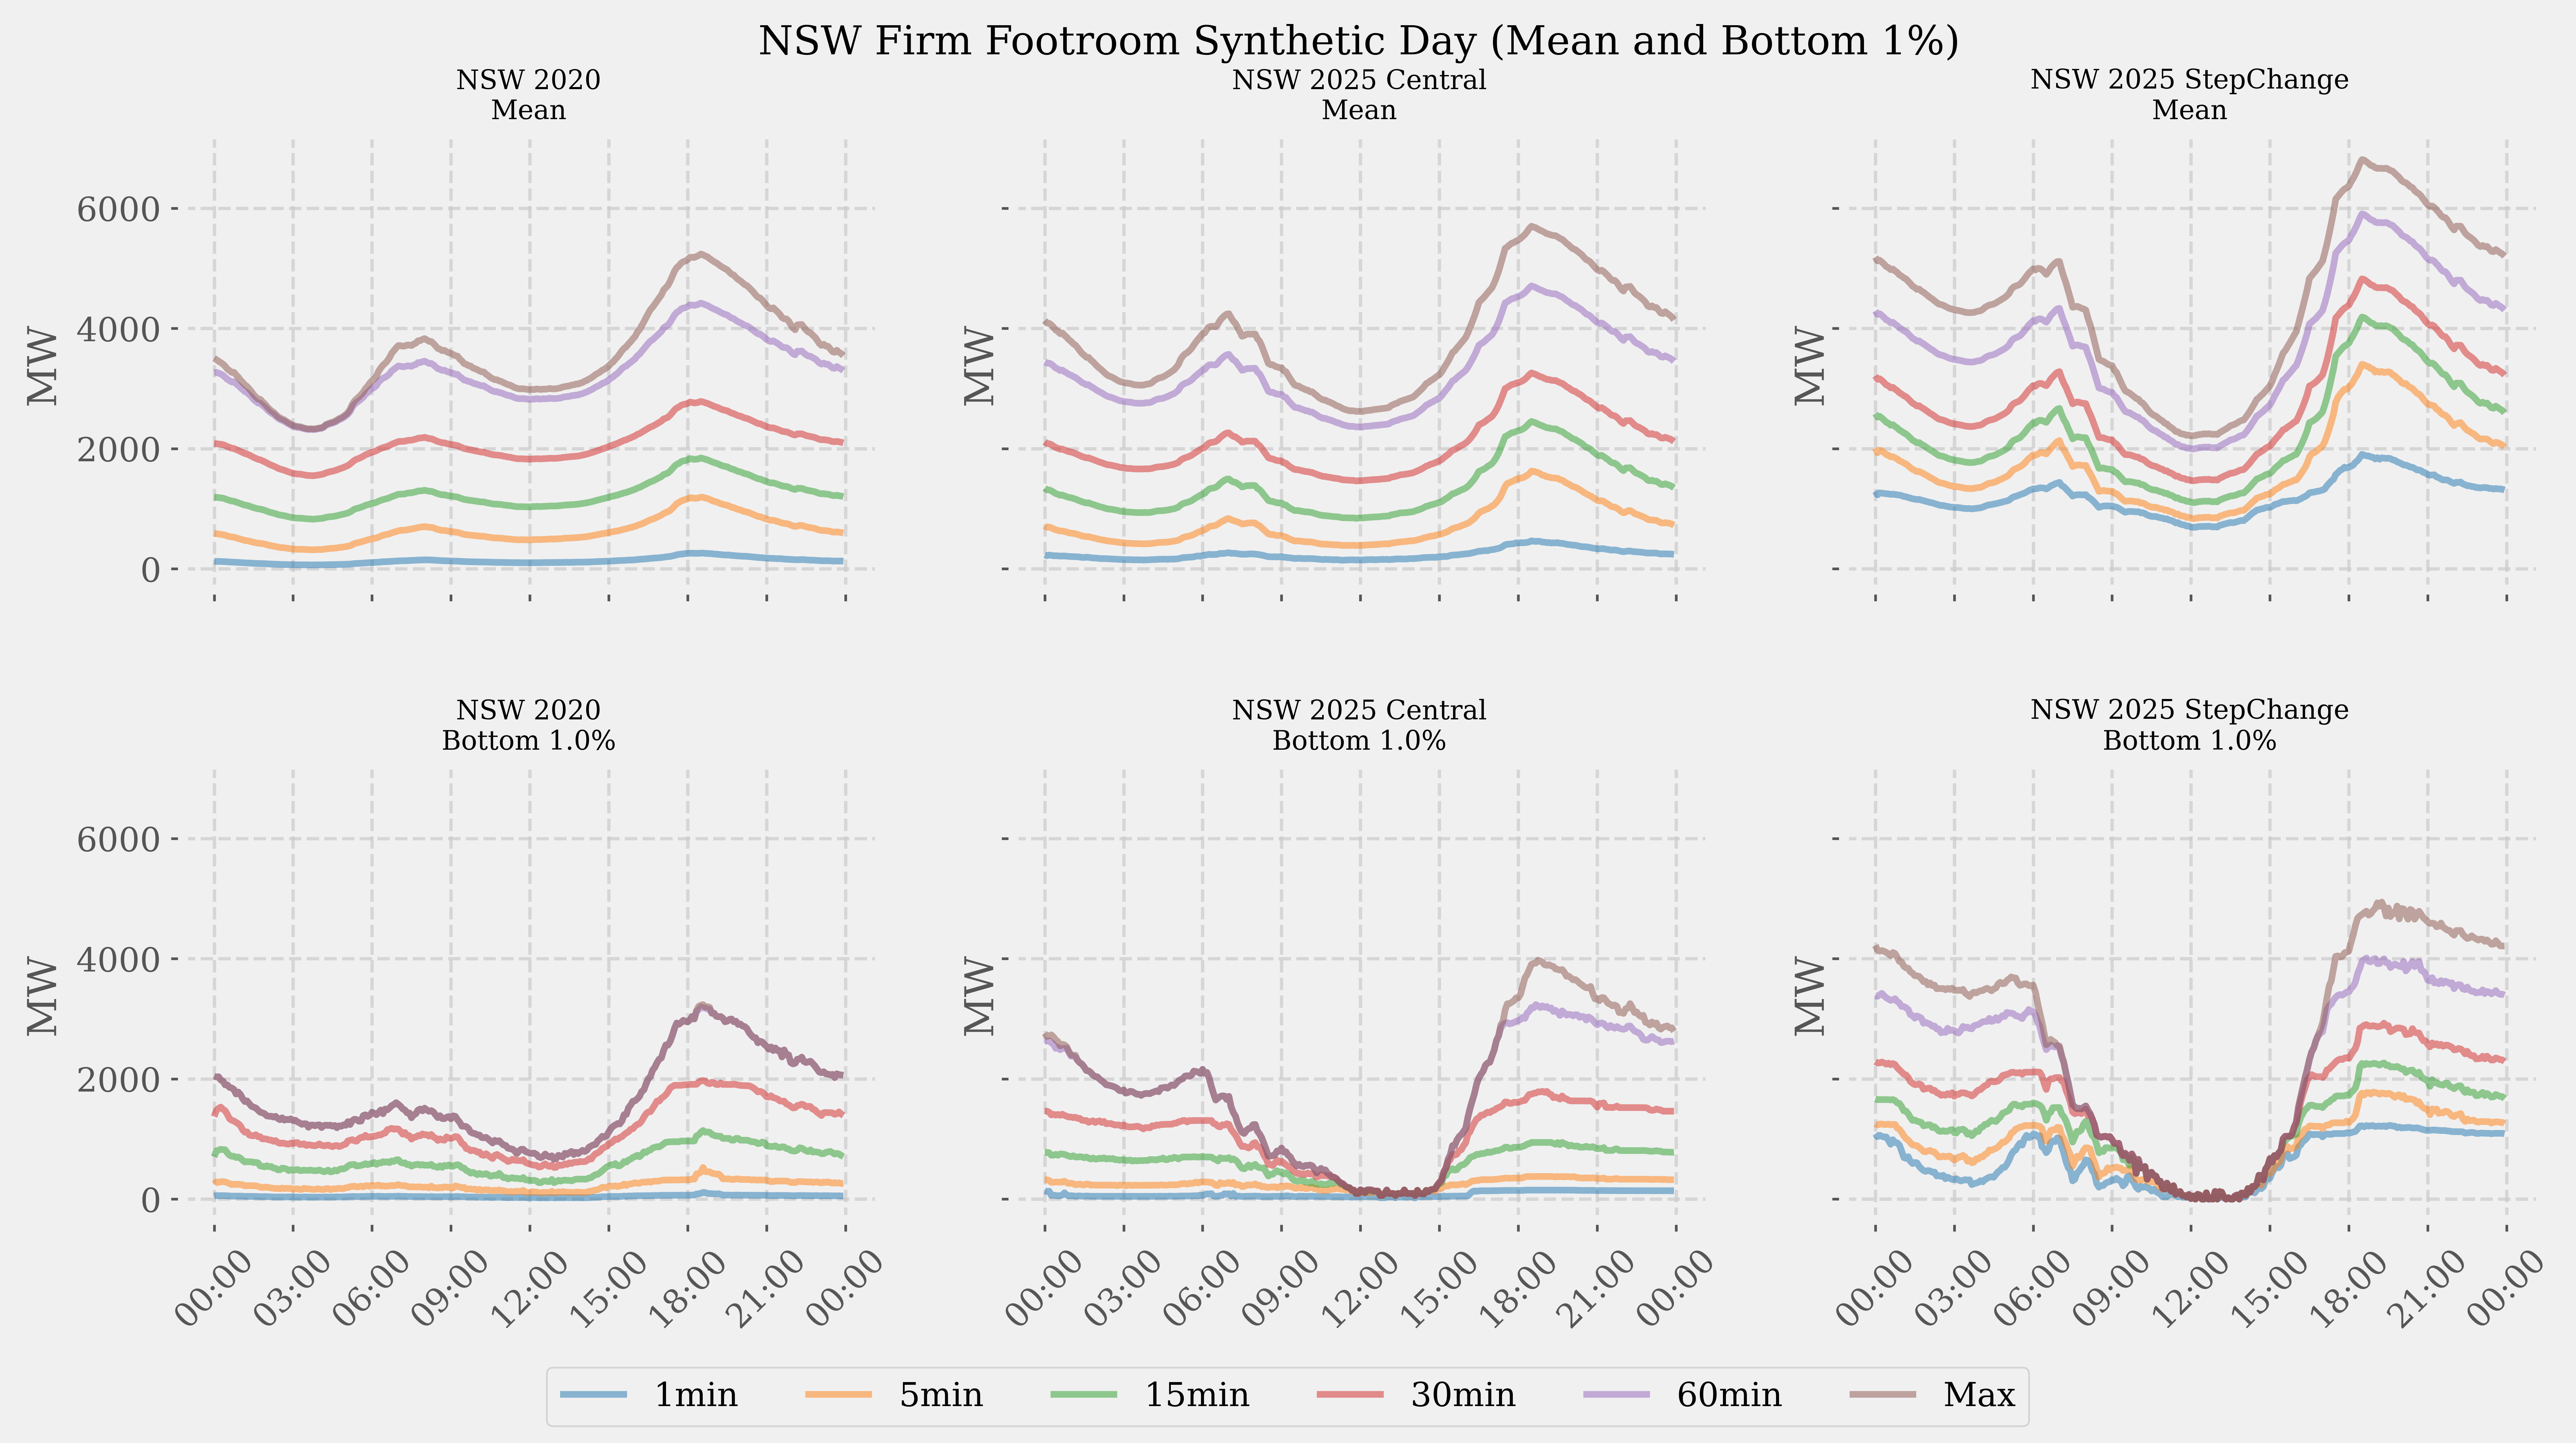
\includegraphics[width=1\textwidth,height=\textheight]{./source/figures/NSW_firmfootroom_all_profiles_by_di.png}
\caption[NSW firm footroom SDPs]{Mean (top row) and bottom 1\% (bottom
row) SDPs for available firm footroom (i.e.~footroom provided only by
``firm'' resources: conventional and BESS) in NSW in 2020 (leftmost
column) and the two 2025 scenarios (rightmost
columns).}\label{fig:nswfirmfoot}
}
\end{figure}

\begin{figure}
\hypertarget{fig:nswfoot}{%
\centering
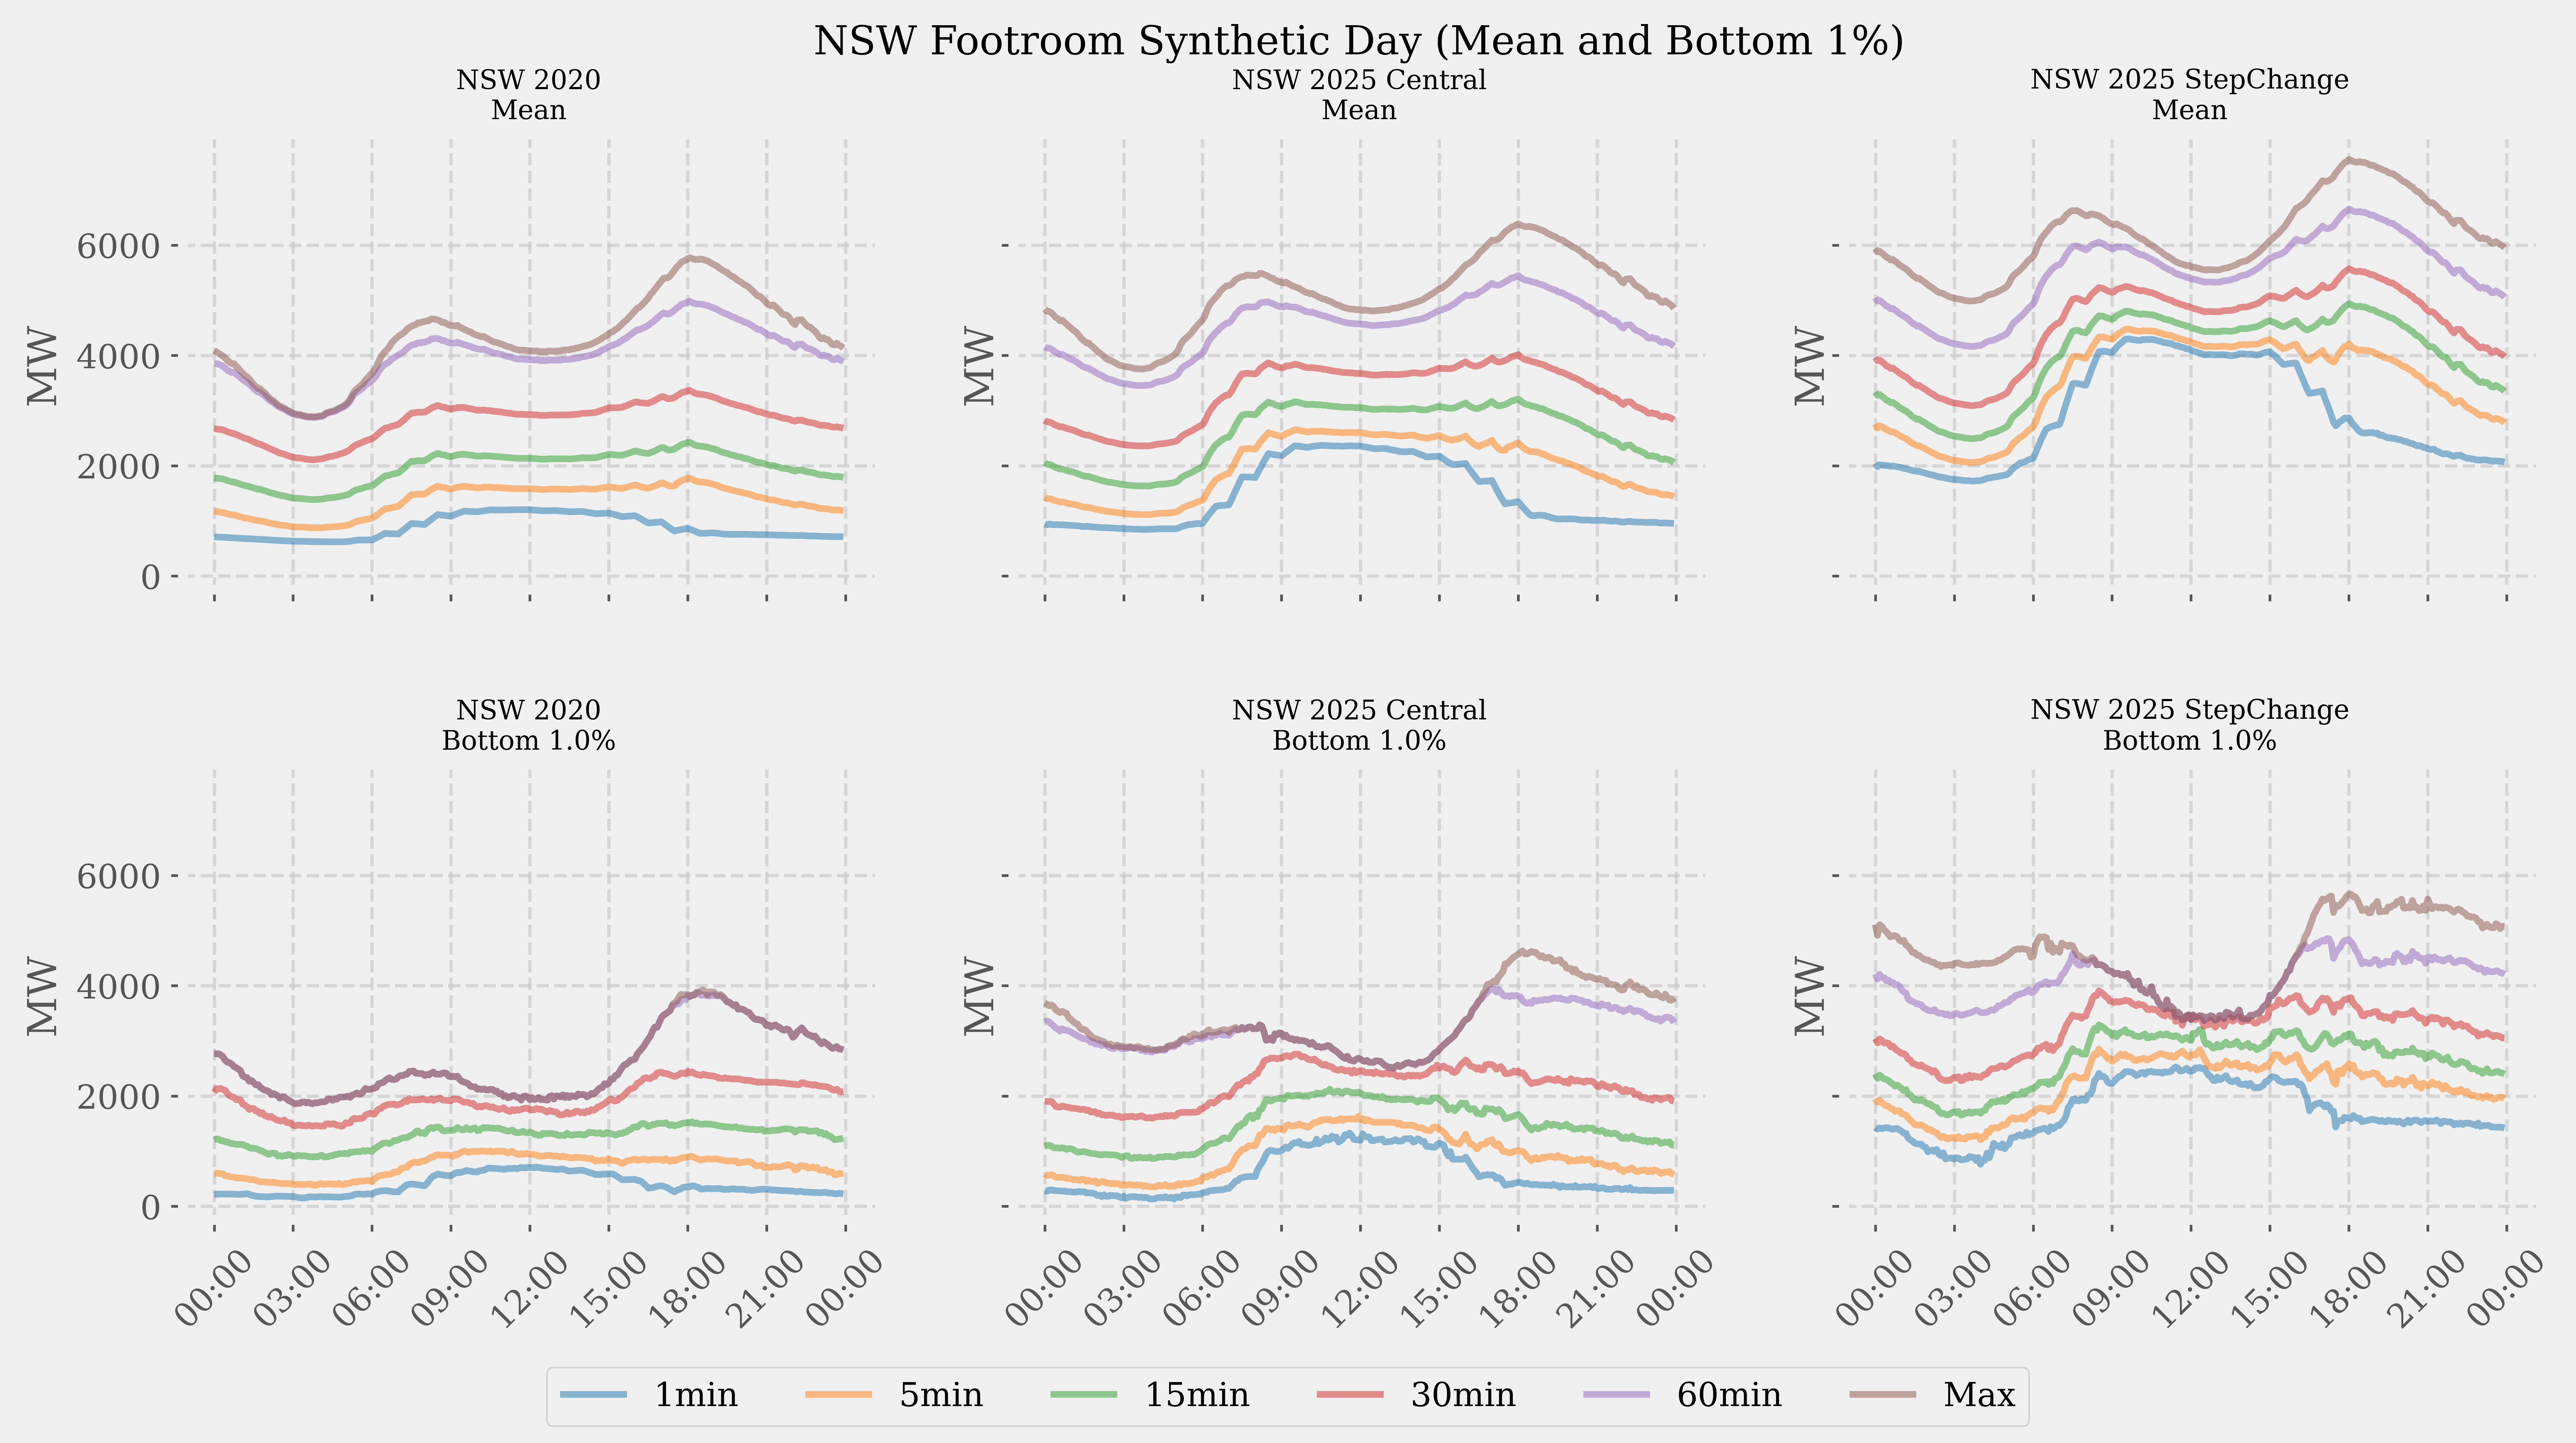
\includegraphics[width=1\textwidth,height=\textheight]{./source/figures/NSW_footroom_all_profiles_by_di.png}
\caption[NSW footroom SDPs]{Mean (top row) and bottom 1\% (bottom row)
SDPs for available total footroom (including footroom that would be
provided by curtailing VRE) in NSW in 2020 (leftmost column) and the two
2025 scenarios (rightmost columns).}\label{fig:nswfoot}
}
\end{figure}

The available footroom in the system is likely sensitive to extent of
conventional generation retirements. Further retirements may enable
remaining conventional resources to operate at a higher loading, thereby
increasing the available footroom in the system. Regardless, given that
each region appears to suffer a lack of \emph{firm} footroom for several
hours during the day in the 2025 scenarios explored in this case study,
mechanisms for procuring sustained downwards balancing flexibility
should be considered alongside those for procuring sustained upwards
balancing flexibility. One simple option would be to implement an
operating \emph{footroom} product, which, if VRE are permitted to
provide this service, can enable conventional generation to operate
closer to their MSL and thus reduce system operating costs and carbon
emissions
(\protect\hyperlink{ref-nelsonInvestigatingEconomicValue2018}{Nelson et
al., 2018}).

\hypertarget{sec:reserves-stelr}{%
\subsubsection{Short-term energy-limited
reserves}\label{sec:reserves-stelr}}

While the available reserves metric does not consider the duration for
which reserve deployment can be sustained, we can infer whether reserves
are short-term energy-limited (i.e.~with a duration no more than a few
hours) based on their resource type. For this analysis, BESS reserve
power was calculated based on the BESS's state of charge at the end of
each dispatch interval and the requirement to sustain provision for 15
minutes. This duration is consistent with the BESS power and capacity
that is reserved in SA for the possibility of loss of interconnection
(\protect\hyperlink{ref-australianenergymarketoperator2020SystemStrength2020}{Australian
Energy Market Operator, 2020o}). In addition, the maximum available
price-responsive demand available in each state was added to the
available reserves in each dispatch interval (assuming an emergency
response time of 5 minutes) to gain a better understanding of the
maximum potential contribution of demand response. This corresponded to
\textasciitilde60 MW in SA and \textasciitilde290 MW in NSW, based on
AEMO analysis and forecasts in Australian Energy Market Operator
(\protect\hyperlink{ref-australianenergymarketoperator2020InputsAssumptions2020}{2020n}).
Both BESS and DR can be considered to be short-term energy-limited
reserve providers. Though conventional generation fuel constraints (e.g
reservoir schemes and the gas system) were not modelled in this market
simulation, the contribution of conventional resources was separated
into those of thermal and hydro to assess the importance of the energy
constraints on each resource type to available reserves in NSW.

Tables \ref{tbl:nsw_stel} and \ref{tbl:sa_stel} show the median
percentage across dispatch intervals in a scenario year of available
reserves provided by a resources type for NSW and SA, respectively.
Whilst hydro and thermal resources dominate 5 minute horizon reserve
provision in 2020 in NSW and SA, respectively, short-term energy limited
resources provide a greater proportion of reserves in this horizon in
2025. In particular, the median contribution of BESS to reserves
available within 5 minutes is 16\% for NSW and 40\% for SA in the 2025
Step Change scenario. As the reserve horizon is extended to 30 minutes,
a greater proportion of reserves are provided by conventional resources,
which may be better positioned to sustain a response beyond the
short-term\footnote{In reality, conventional resources are also
  susceptible to fuel constraints, as highlighted by the events
  preceding the 2022 NEM suspension
  (\protect\hyperlink{ref-australianenergymarketoperatorNEMMarketSuspension2022}{Australian
  Energy Market Operator, 2022c}). More sophisticated modelling of
  thermal coal availability, the gas system and hydro schemes, including
  their operation under different climate conditions, would be required
  to better understand the potential duration of available reserve
  provided by conventional generation.}. These results indicate that as
energy transition progresses, a trade-off between reserve deployment
speed and duration develops. This trend reaffirms the value of the
sequential and hierarchical approach to reserve product design and
deployment that has been adopted in many jurisdictions
(\protect\hyperlink{ref-prakashInsightsDesigningEffective2022}{Prakash
et al., 2022}). Moreover, it should be noted that unlike other
mechanisms for procuring balancing flexibility, reserve services and
products can specify duration/energy requirements and thus ensure that
flexibility provision is sustained.

\def\pandoctableshortcapt{NSW short-term energy limited reserves}

\hypertarget{tbl:nsw_stel}{}
\begin{longtable}[]{@{}
  >{\centering\arraybackslash}m{(\columnwidth - 12\tabcolsep) * \real{0.2366}}
  >{\centering\arraybackslash}m{(\columnwidth - 12\tabcolsep) * \real{0.1183}}
  >{\centering\arraybackslash}m{(\columnwidth - 12\tabcolsep) * \real{0.1183}}
  >{\centering\arraybackslash}m{(\columnwidth - 12\tabcolsep) * \real{0.1183}}
  >{\centering\arraybackslash}m{(\columnwidth - 12\tabcolsep) * \real{0.1183}}
  >{\centering\arraybackslash}m{(\columnwidth - 12\tabcolsep) * \real{0.1183}}
  >{\centering\arraybackslash}m{(\columnwidth - 12\tabcolsep) * \real{0.1183}}@{}}
\caption[NSW short-term energy limited
reserves]{\label{tbl:nsw_stel}Median of the percentage of each resource
type's contribution to reserves available within 5 minutes and 30
minutes in every dispatch interval for each NSW scenario year. The
median percentages are not necessarily coincident (i.e.~from the same
dispatch interval) and therefore may not sum to 100\%. Furthermore, some
distributions are long-tailed, so a median does not capture occasional
reserve provision by a resource type (e.g.~VRE, for which all medians
are 0\%).}\tabularnewline
\toprule\noalign{}
\multirow{2}{=}{\begin{minipage}[b]{\linewidth}\centering
NSW resources
\end{minipage}} &
\multicolumn{2}{>{\centering\arraybackslash}m{(\columnwidth - 12\tabcolsep) * \real{0.2366} + 2\tabcolsep}}{%
\begin{minipage}[b]{\linewidth}\centering
2020
\end{minipage}} &
\multicolumn{2}{>{\centering\arraybackslash}m{(\columnwidth - 12\tabcolsep) * \real{0.2366} + 2\tabcolsep}}{%
\begin{minipage}[b]{\linewidth}\centering
2025 Central
\end{minipage}} &
\multicolumn{2}{>{\centering\arraybackslash}m{(\columnwidth - 12\tabcolsep) * \real{0.2366} + 2\tabcolsep}@{}}{%
\begin{minipage}[b]{\linewidth}\centering
2025 Step Change
\end{minipage}} \\
& \begin{minipage}[b]{\linewidth}\centering
5 min
\end{minipage} & \begin{minipage}[b]{\linewidth}\centering
30 min
\end{minipage} & \begin{minipage}[b]{\linewidth}\centering
5 min
\end{minipage} & \begin{minipage}[b]{\linewidth}\centering
30 min
\end{minipage} & \begin{minipage}[b]{\linewidth}\centering
5 min
\end{minipage} & \begin{minipage}[b]{\linewidth}\centering
30 min
\end{minipage} \\
\midrule\noalign{}
\endfirsthead
\toprule\noalign{}
\multirow{2}{=}{\begin{minipage}[b]{\linewidth}\centering
NSW resources
\end{minipage}} &
\multicolumn{2}{>{\centering\arraybackslash}m{(\columnwidth - 12\tabcolsep) * \real{0.2366} + 2\tabcolsep}}{%
\begin{minipage}[b]{\linewidth}\centering
2020
\end{minipage}} &
\multicolumn{2}{>{\centering\arraybackslash}m{(\columnwidth - 12\tabcolsep) * \real{0.2366} + 2\tabcolsep}}{%
\begin{minipage}[b]{\linewidth}\centering
2025 Central
\end{minipage}} &
\multicolumn{2}{>{\centering\arraybackslash}m{(\columnwidth - 12\tabcolsep) * \real{0.2366} + 2\tabcolsep}@{}}{%
\begin{minipage}[b]{\linewidth}\centering
2025 Step Change
\end{minipage}} \\
& \begin{minipage}[b]{\linewidth}\centering
5 min
\end{minipage} & \begin{minipage}[b]{\linewidth}\centering
30 min
\end{minipage} & \begin{minipage}[b]{\linewidth}\centering
5 min
\end{minipage} & \begin{minipage}[b]{\linewidth}\centering
30 min
\end{minipage} & \begin{minipage}[b]{\linewidth}\centering
5 min
\end{minipage} & \begin{minipage}[b]{\linewidth}\centering
30 min
\end{minipage} \\
\midrule\noalign{}
\endhead
\bottomrule\noalign{}
\endlastfoot
BESS (15 min) & 0\% & 0\% & 2\% & 1\% & 16\% & 14\% \\
DR & 9\% & 5\% & 5\% & 4\% & 5\% & 4\% \\
Hydro & 74\% & 43\% & 81\% & 60\% & 71\% & 61\% \\
Thermal & 18\% & 52\% & 12\% & 34\% & 8\% & 19\% \\
\end{longtable}

\let\pandoctableshortcapt\relax

\def\pandoctableshortcapt{SA short-term energy limited reserves}

\hypertarget{tbl:sa_stel}{}
\begin{longtable}[]{@{}
  >{\centering\arraybackslash}m{(\columnwidth - 12\tabcolsep) * \real{0.2366}}
  >{\centering\arraybackslash}m{(\columnwidth - 12\tabcolsep) * \real{0.1183}}
  >{\centering\arraybackslash}m{(\columnwidth - 12\tabcolsep) * \real{0.1183}}
  >{\centering\arraybackslash}m{(\columnwidth - 12\tabcolsep) * \real{0.1183}}
  >{\centering\arraybackslash}m{(\columnwidth - 12\tabcolsep) * \real{0.1183}}
  >{\raggedright\arraybackslash}m{(\columnwidth - 12\tabcolsep) * \real{0.1183}}
  >{\centering\arraybackslash}m{(\columnwidth - 12\tabcolsep) * \real{0.1183}}@{}}
\caption[SA short-term energy limited
reserves]{\label{tbl:sa_stel}Median of the percentage of each resource
type's contribution to reserves available within 5 minutes and 30
minutes in every dispatch interval for each SA scenario year. The median
percentages are not necessarily coincident (i.e.~from the same dispatch
interval) and therefore may not sum to 100\%. Furthermore, some
distributions are long-tailed, so a median does not capture occasional
reserve provision by a resource type (e.g.~VRE, for which all medians
are 0\%).}\tabularnewline
\toprule\noalign{}
\multirow{2}{=}{\begin{minipage}[b]{\linewidth}\centering
SA resources
\end{minipage}} &
\multicolumn{2}{>{\centering\arraybackslash}m{(\columnwidth - 12\tabcolsep) * \real{0.2366} + 2\tabcolsep}}{%
\begin{minipage}[b]{\linewidth}\centering
2020
\end{minipage}} &
\multicolumn{2}{>{\centering\arraybackslash}m{(\columnwidth - 12\tabcolsep) * \real{0.2366} + 2\tabcolsep}}{%
\begin{minipage}[b]{\linewidth}\centering
2025 Central
\end{minipage}} &
\multicolumn{2}{>{\raggedright\arraybackslash}m{(\columnwidth - 12\tabcolsep) * \real{0.2366} + 2\tabcolsep}@{}}{%
\begin{minipage}[b]{\linewidth}\raggedright
2025 Step Change
\end{minipage}} \\
& \begin{minipage}[b]{\linewidth}\centering
5 min
\end{minipage} & \begin{minipage}[b]{\linewidth}\centering
30 min
\end{minipage} & \begin{minipage}[b]{\linewidth}\centering
5 min
\end{minipage} & \begin{minipage}[b]{\linewidth}\centering
30 min
\end{minipage} & \begin{minipage}[b]{\linewidth}\raggedright
5 min
\end{minipage} & \begin{minipage}[b]{\linewidth}\centering
30 min
\end{minipage} \\
\midrule\noalign{}
\endfirsthead
\toprule\noalign{}
\multirow{2}{=}{\begin{minipage}[b]{\linewidth}\centering
SA resources
\end{minipage}} &
\multicolumn{2}{>{\centering\arraybackslash}m{(\columnwidth - 12\tabcolsep) * \real{0.2366} + 2\tabcolsep}}{%
\begin{minipage}[b]{\linewidth}\centering
2020
\end{minipage}} &
\multicolumn{2}{>{\centering\arraybackslash}m{(\columnwidth - 12\tabcolsep) * \real{0.2366} + 2\tabcolsep}}{%
\begin{minipage}[b]{\linewidth}\centering
2025 Central
\end{minipage}} &
\multicolumn{2}{>{\raggedright\arraybackslash}m{(\columnwidth - 12\tabcolsep) * \real{0.2366} + 2\tabcolsep}@{}}{%
\begin{minipage}[b]{\linewidth}\raggedright
2025 Step Change
\end{minipage}} \\
& \begin{minipage}[b]{\linewidth}\centering
5 min
\end{minipage} & \begin{minipage}[b]{\linewidth}\centering
30 min
\end{minipage} & \begin{minipage}[b]{\linewidth}\centering
5 min
\end{minipage} & \begin{minipage}[b]{\linewidth}\centering
30 min
\end{minipage} & \begin{minipage}[b]{\linewidth}\raggedright
5 min
\end{minipage} & \begin{minipage}[b]{\linewidth}\centering
30 min
\end{minipage} \\
\midrule\noalign{}
\endhead
\bottomrule\noalign{}
\endlastfoot
BESS (15 min) & 14\% & 6\% & 24\% & 10\% & 40\% & 20\% \\
DR & 7\% & 3\% & 7\% & 3\% & 5\% & 3\% \\
Thermal & 71\% & 88\% & 61\% & 84\% & 45\% & 73\% \\
\end{longtable}

\let\pandoctableshortcapt\relax

\hypertarget{the-role-of-balancing-products}{%
\subsection{The role of balancing
products}\label{the-role-of-balancing-products}}

It is unclear whether introducing an operating reserve product will
deliver material operational benefits to the NEM in light of the revenue
risks, complexity, and implementation and ongoing costs associated with
a new market. Instead, existing mechanisms may be able to deliver
sufficient upwards flexibility, particularly if they can be augmented:

\begin{enumerate}
\def\labelenumi{\arabic{enumi}.}
\item
  Market participants with forward market obligations are strongly
  incentivised to offer balancing flexibility to the market. The premium
  payment offered to the seller, along with a strong financial incentive
  to perform during periods of system stress, means that derivatives
  such as cap contracts somewhat resemble pay-for-performance capacity
  remuneration mechanisms\footnote{However, derivatives are financial in
    nature and thus need not be ``backed'' by power system resources
    (i.e.~they are not associated with any physical obligation).}.
  Participants would have further incentive if contracting were made
  mandatory (\protect\hyperlink{ref-maysPrivateRiskSocial2022}{Mays et
  al., 2022}), or if they increasingly resort to contracting to hedge
  pricing volatility that could occur as energy transition progresses
  (\protect\hyperlink{ref-devriesMarketSignalsAdequacy2022}{de Vries and
  Sanchez Jimenez, 2022}).
\item
  Market and system information and forecasts (e.g.~the NEM's ahead
  processes) may be critical to ensuring that market participants
  schedule resources to provide flexibility to the system. Future work
  should not only seek to improve their accuracy and their treatment of
  uncertainties, but also to understand how they shape participant
  decision-making and thus which enhancements could provide the most
  value.
\end{enumerate}

However, there remain some operational benefits of additional balancing
products. Nested distribution-level markets and/or real-time market
scheduling of aggregated resources have the potential to better enable
balancing flexibility from DER. However, a key insight from
Section~\ref{sec:reserves-stelr} is that consideration should be given
to the duration of this flexibility. System stress could coincide with
periods in which DER owners wish to use these resources for themselves
(e.g.~a heatwave or if they are exposed to real-time market volatility
to some extent)
(\protect\hyperlink{ref-robertsVPPUserResearch2020}{Roberts et al.,
2020}). In contrast, reserve products that specify response durations
could provide the SO with certainty that flexibility is only procured
from resources that are available for a minimum period of time. Any
duration requirements would need to be balanced against the quantity and
diversity of flexibility providers -- primarily to ensure that product
markets are competitive, but also because successive deployment of
several short-term energy limited resources may be sufficient to meet
system balancing needs over the course of a few hours. Furthermore,
sustained footroom products might assist SOs in managing a lack of firm
footroom (Section~\ref{sec:reserves-footroomSDPs}). Typically, energy
prices rise when upwards flexibility is scarce, thereby compensating
providers of upward flexibility. In contrast, downwards flexibility
providers are not strictly compensated through energy pricing, as
oversupply could lead to dispatch curtailing, rather than remunerating
flexible resources. Though this might mean flexible resources avoid
financial losses, it comes at the cost of footroom available to the
system. Accordingly, an ``operating footroom'' product that remunerates
downwards flexibility offers a solution to the tension between dispatch
incentives and the need for system footroom.

\hypertarget{sec:reserves-conclusion}{%
\section{Conclusion and policy
implications}\label{sec:reserves-conclusion}}

State-of-the-art resource adequacy assessments are closing the gap
between traditional capacity adequacy assessments, which focus on
capacity reserve margins during peak demand events, and flexibility
adequacy assessments that often model chronological operations
(\protect\hyperlink{ref-stenclikQuantifyingRiskUncertain2021}{Stenclik
et al., 2021}). Yet flexibility adequacy assessments alone do not
necessarily offer a better understanding of \emph{what type} of
balancing flexibility a system has and might need, and \emph{how} best
to make it available to the system. As resource mixes change
dramatically during energy transition, system designers, planners and
operators should quantify balancing flexibility capabilities to gain an
appreciation of the availability of different resource types to inform
operational practice design.

By quantifying balancing flexibility ``margins'' in two sub-systems of
the Australian National Electricity Market
(Section~\ref{sec:reserves-casestudy}), we identify potential balancing
flexibility dynamics and trends in future power systems. Firstly,
systems with high penetrations of distributed and utility-scale solar PV
will likely have reserve ``surpluses'' around the middle of the day and
periods of relative reserve scarcity during morning and evening peak
demand events. In such systems, the periods when reserves are most
valuable do not necessarily correspond to the periods during which it is
most efficient to curtail renewable energy generation (due to oversupply
or to obtain reserves). As such, a key recommendation for policy-makers
is to consider whether reserve product markets are needed to elicit
sufficient balancing flexibility provision during these short periods of
relative scarcity, or whether adjusting energy market settings, forward
market obligations and/or market and system information processes can
achieve this. Understanding the potential benefits of new reserve
product markets is crucial because they can introduce additional costs,
constraints and complexity whilst encroaching upon the functions of
other operational practices. Secondly, our study highlights the
importance of placing a greater emphasis on duration, as resources
touted as essential future balancing flexibility providers (e.g.~battery
energy storage, demand response) may only be able to sustain a response
for at most a few hours. Thirdly, we highlight the need to consider
footroom and the benefits of enabling renewable energy to provide it.
Footroom procurement and response duration specifications are
underappreciated by prevailing market designs, and may be better
addressed by policy-makers either modifying existing or creating new
reserve product specifications.

\hypertarget{sec:fourth}{%
\chapter{Final research study}\label{sec:fourth}}

\hypertarget{introduction-3}{%
\section{Introduction}\label{introduction-3}}

This is the introduction. Nunc lorem odio, laoreet eu turpis at,
condimentum sagittis diam. Phasellus metus ligula, auctor ac nunc vel,
molestie mattis libero. Praesent id posuere ex, vel efficitur nibh.
Quisque vestibulum accumsan lacus vitae mattis.

\hypertarget{method-1}{%
\section{Method}\label{method-1}}

In tincidunt viverra dolor, ac pharetra tellus faucibus eget.
Pellentesque tempor a enim nec venenatis. Morbi blandit magna imperdiet
posuere auctor. Maecenas in maximus est.

\hypertarget{results-1}{%
\section{Results}\label{results-1}}

These are the results. Curabitur vulputate nisl non ante tincidunt
tempor. Aenean porta nisi quam, sed ornare urna congue sed. Curabitur in
sapien justo. Quisque pulvinar ullamcorper metus, eu varius mauris
pellentesque et. In hac habitasse platea dictumst. Pellentesque nec
porttitor libero. Duis et magna a massa lacinia cursus.

\hypertarget{discussion-1}{%
\section{Discussion}\label{discussion-1}}

This is the discussion. Curabitur gravida nisl id gravida congue. Duis
est nisi, sagittis eget accumsan ullamcorper, semper quis turpis. Mauris
ultricies diam metus, sollicitudin ultricies turpis lobortis vitae. Ut
egestas vehicula enim, porta molestie neque consectetur placerat.
Integer iaculis sapien dolor, non porta nibh condimentum ut.

\hypertarget{conclusion-3}{%
\section{Conclusion}\label{conclusion-3}}

This is the conclusion to the chapter. Nulla sed condimentum lectus.
Duis sed tempor erat, at cursus lacus. Nam vitae tempus arcu, id
vestibulum sapien. Cum sociis natoque penatibus et magnis dis parturient
montes, nascetur ridiculus mus.

\hypertarget{sec:conclusion}{%
\chapter{Conclusion}\label{sec:conclusion}}

\hypertarget{thesis-summary}{%
\section{Thesis summary}\label{thesis-summary}}

In summary, pellentesque habitant morbi tristique senectus et netus et
malesuada fames ac turpis egestas. Nunc eleifend, ex a luctus porttitor,
felis ex suscipit tellus, ut sollicitudin sapien purus in libero. Nulla
blandit eget urna vel tempus. Praesent fringilla dui sapien, sit amet
egestas leo sollicitudin at.

\hypertarget{future-work}{%
\section{Future work}\label{future-work}}

There are several potential directions for extending this thesis. Lorem
ipsum dolor sit amet, consectetur adipiscing elit. Aliquam gravida ipsum
at tempor tincidunt. Aliquam ligula nisl, blandit et dui eu, eleifend
tempus nibh. Nullam eleifend sapien eget ante hendrerit commodo.
Pellentesque pharetra erat sit amet dapibus scelerisque.

Vestibulum suscipit tellus risus, faucibus vulputate orci lobortis eget.
Nunc varius sem nisi. Nunc tempor magna sapien, euismod blandit elit
pharetra sed. In dapibus magna convallis lectus sodales, a consequat sem
euismod. Curabitur in interdum purus. Integer ultrices laoreet aliquet.
Nulla vel dapibus urna. Nunc efficitur erat ac nisi auctor sodales.

\appendix

\#

\renewcommand\thefigure{\thesection.\arabic{figure}} 
\renewcommand\thetable{\thesection.\arabic{table}}

\hypertarget{data-and-assumptions-used-in-market-simulation}{%
\chapter{Data and assumptions used in market
simulation}\label{data-and-assumptions-used-in-market-simulation}}

\hypertarget{resource-ramp-rates}{%
\section{Resource ramp rates}\label{resource-ramp-rates}}

Separate upwards and downwards ramp rates were modelled for most
resource types. For hydro generation and reciprocating engines, maximum
upwards and downwards ramp rates were sourced from GHD
(\protect\hyperlink{ref-ghd2018AEMOCost2018}{2018}). For other
conventional resources (coal-fired generation, Gas-Steam, CCGT and
OCGT), ramp rates in each direction were further separated into a
\emph{market} ramp rate, which was used in the PLEXOS market simulation,
and an \emph{upper} ramp rate, which was used to calculate available
reserves/footroom. For these resources, the market ramp rate was
calculated using the unit ramp rates used most frequently in NEM
dispatch\footnote{AEMO is currently investigating appropriate regional
  requirements for FCAS, particularly for contingency FCAS in the
  terminal regions of QLD and SA
  (\protect\hyperlink{ref-australianenergymarketoperatorRenewableIntegrationStudy2020b}{Australian
  Energy Market Operator, 2020h},
  \protect\hyperlink{ref-australianenergymarketoperatorElectricityRuleChange2019a}{2019d}).}
in 2020, and the upper ramp rate was calculated using resources' assumed
maximum ramp rates in AEMO's 2020 Inputs and Assumptions workbook (for
an example of a comparison, see Figure~\ref{fig:ramp_rate_comparison})
(\protect\hyperlink{ref-australianenergymarketoperator2020InputsAssumptions2020}{Australian
Energy Market Operator, 2020n}). Additional resources in 2025 were
assumed to have the same ramp rate characteristics as newer existing
resources of the same technology type.

\begin{figure}
\hypertarget{fig:ramp_rate_comparison}{%
\centering
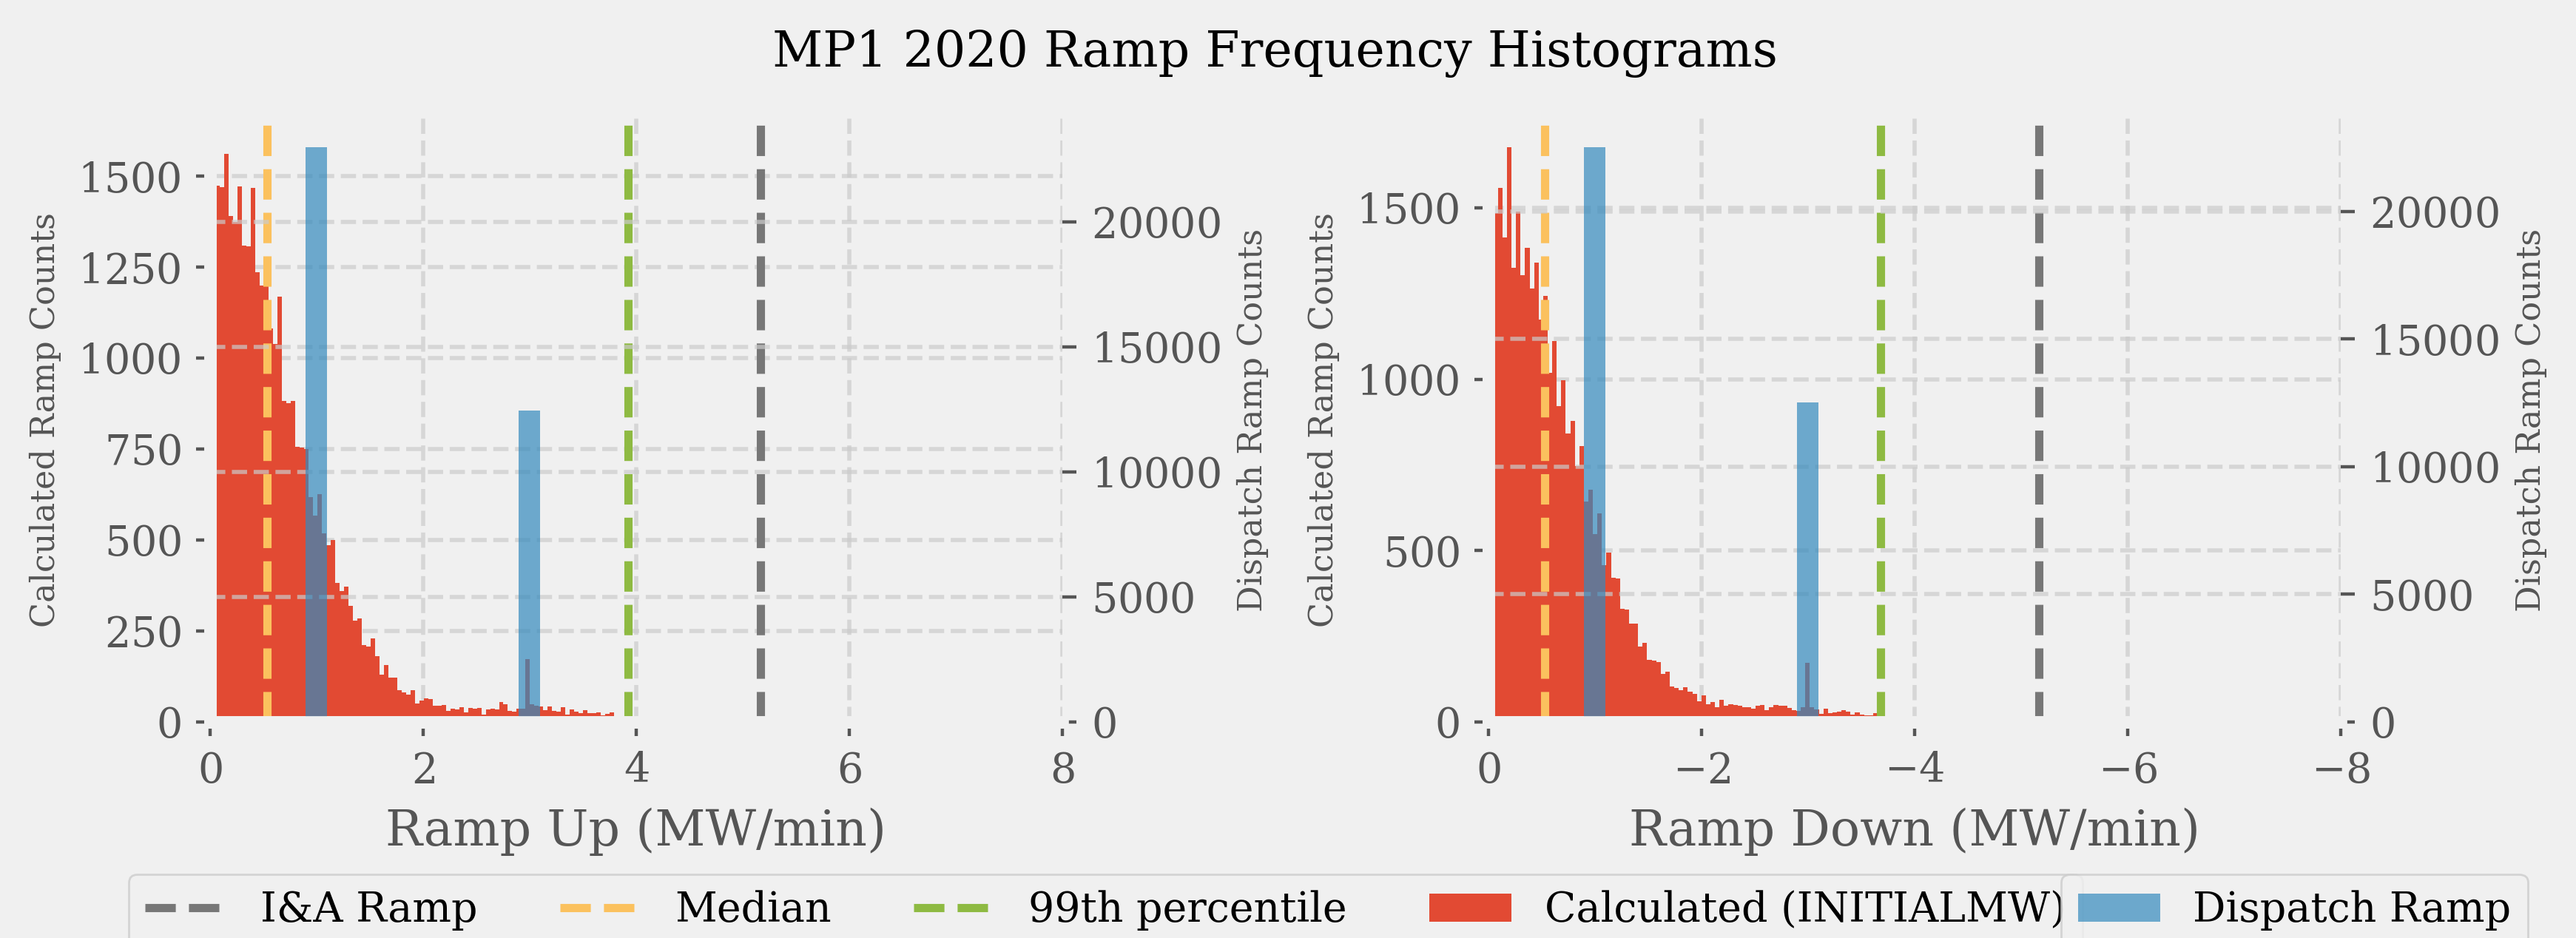
\includegraphics{source/figures/coal_market_upper_ramps.png}
\caption[Observed, submitted and ISP ramp rates for a NSW coal-fired
unit]{Ramp rates observed (red) and used in dispatch by AEMO (blue) for
a coal-fired unit in NSW in 2020. The green line denotes the ramp rate
assumed by AEMO in its 2020 Inputs and Assumptions workbook and the 2020
ISP.}\label{fig:ramp_rate_comparison}
}
\end{figure}

\hypertarget{unit-commitment-and-cycling-constraints}{%
\section{Unit commitment and cycling
constraints}\label{unit-commitment-and-cycling-constraints}}

Many existing flexible conventional resources (OCGT, reciprocating
engines and hydro generation) submit dispatch inflexibility profiles to
AEMO that contain the resource's time to start up and reach MSL, the MSL
itself, the time required at minimum loading and the time taken to shut
down
(\protect\hyperlink{ref-australianenergymarketoperatorFastStartInflexibilityProfile2021}{Australian
Energy Market Operator, 2021q}). The most frequently offered fast start
inflexibility profile of a resource in 2020 was obtained using NEMOSIS
(\protect\hyperlink{ref-gormanNEMOSISNEMOpen2018}{Gorman et al., 2018})
and used to calculate its start-up rate, minimum up-time, MSL and
shutdown rate. The minimum down-time for these resources was chosen to
be equal to the minimum up-time.

For the other conventional resources (CCGT, coal-fired generation and
Gas-Steam), minimum up-times, minimum down-times and MSLs were obtained
from AEMO's 2020 Inputs and Assumptions workbook
(\protect\hyperlink{ref-australianenergymarketoperator2020InputsAssumptions2020}{Australian
Energy Market Operator, 2020n}) and start-up rates were calculated based
on hot or warm start times (i.e.~depending on the start state of the
resource after being offline for its minimum down-time) obtained from
GHD (\protect\hyperlink{ref-ghd2018AEMOCost2018}{2018}) or Aurecon
Australasia
(\protect\hyperlink{ref-aureconaustralasiaGeneratorTechnicalCost2020}{2020}).
The shut-down rates for these resources were calculated based on actual
shutdowns, or those of similar technology types, observed in AEMO
dispatch data that was obtained using NEMOSIS
(\protect\hyperlink{ref-gormanNEMOSISNEMOpen2018}{Gorman et al., 2018}).

BESS were dispatched by PLEXOS's arbitrage algorithm subject to charging
and discharging efficiencies and maximum and minimum state of charge
constraints that corresponded to those assumed within AEMO's 2020 Inputs
and Assumptions workbook
(\protect\hyperlink{ref-australianenergymarketoperator2020InputsAssumptions2020}{Australian
Energy Market Operator, 2020n}). Given an assumed economic lifetime of
10 years
(\protect\hyperlink{ref-australianenergymarketoperator2020InputsAssumptions2020}{Australian
Energy Market Operator, 2020n}) and 3000 cycles
(\protect\hyperlink{ref-dasilvalimaLifeCycleAssessment2021}{da Silva
Lima et al., 2021}) for lithium-ion BESS, a constraint of 300 cycles per
year was applied to BESS in each scenario.

\hypertarget{partial-and-forced-outages}{%
\section{Partial and forced outages}\label{partial-and-forced-outages}}

Maintenance rates, forced outage rates (partial and full) and the
corresponding mean time taken to repair were modelled for all
conventional generation and were sourced from AEMO's 2020 Inputs and
Assumptions workbook
(\protect\hyperlink{ref-australianenergymarketoperator2020InputsAssumptions2020}{Australian
Energy Market Operator, 2020n}).

\hypertarget{sa-synchronous-generation-requirement}{%
\section{SA synchronous generation
requirement}\label{sa-synchronous-generation-requirement}}

At present, certain combinations of synchronous generators are required
to remain online for power system security in SA. Should ahead processes
indicate that the synchronous generation expected to be online and
dispatched is inadequate to provide sufficient system strength in SA,
AEMO will intervene in the market and direct additional synchronous
generation online (\protect\hyperlink{ref-guReviewSystemStrength2019}{Gu
et al., 2019}). The various sufficient combinations of synchronous
generation in SA are outlined in Australian Energy Market Operator
(\protect\hyperlink{ref-australianenergymarketoperatorTransferLimitAdvice2022}{2022d}),
with a decrease in requirements/increase in the allowable asynchronous
generation level following the installation of 4 synchronous condensers
(completed in 2021). To model these requirements, a must-run condition
was imposed on 3 CCGT units and 1 Gas-Steam unit in 2020, and on 2 CCGT
units and 1 Gas-Steam unit in the 2025 scenarios. These combinations
reflect a subset of the sufficient combinations outlined in Australian
Energy Market Operator
(\protect\hyperlink{ref-australianenergymarketoperatorTransferLimitAdvice2022}{2022d}).

\hypertarget{hydro-generation-monthly-energy-constraints}{%
\section{Hydro generation monthly energy
constraints}\label{hydro-generation-monthly-energy-constraints}}

Run-of-river hydro generation and pumped hydro storage in NSW were
aggregated and modelled as dispatchable generation with monthly energy
constraints. These monthly energy constraints correspond to the average
monthly inflows for the Snowy scheme (NSW and Australia's largest hydro
scheme) across financial years 2011 to 2018 (obtained from Australian
Energy Market Operator
(\protect\hyperlink{ref-australianenergymarketoperator2020InputsAssumptions2020}{2020n})).
Though this model for hydro does not account for the additional
generation that could be extracted from pumped storage, the application
of monthly energy constraints could be interpreted as modelling one
pattern of run-of-river hydro operation and/or enforcing the same
reservoir level at the start and end of each month (and thus at the
start and end of each year). Explicitly modelling reservoir schemes,
inflows for individual hydro generators and pumping opportunities for
pumped hydro storage are likely to improve the accuracy of the
methodology proposed in this work for systems with significant shares of
hydropower capacity.

\hypertarget{demand-and-vre-traces}{%
\section{Demand and VRE traces}\label{demand-and-vre-traces}}

Chronological demand traces at 5-minute resolution were used in the
market simulation. For each region, historical operational demand for
2020 at 5-minute resolution was obtained using NEMOSIS
(\protect\hyperlink{ref-gormanNEMOSISNEMOpen2018}{Gorman et al., 2018})
and used as the demand trace for the 2020 scenario. AEMO ISP demand
traces were available for each 2025 scenario at half-hourly resolution
(\protect\hyperlink{ref-australianenergymarketoperator2020DraftISP2019a}{Australian
Energy Market Operator, 2019f}); 5-minute resolution demand traces for
each 2025 scenario were produced by scaling 5-minute historical
operational demand by a corresponding half-hourly scaling factor, which
was calculated as the ratio of the ISP scenario's 2025 demand trace to
the ISP scenario's 2020 demand trace.

Half-hourly chronological solar PV and wind capacity factor traces were
obtained from AEMO's ISP database for each 2020 scenario
(\protect\hyperlink{ref-australianenergymarketoperator2020DraftISP2019}{Australian
Energy Market Operator, 2019g}) and for each 2025 scenario
(\protect\hyperlink{ref-australianenergymarketoperator2020ISPSolar2020}{Australian
Energy Market Operator, 2020p}). Generation traces were obtained by
multiplying the capacity factor trace of a resource by its nameplate
capacity. Capacities for existing and committed VRE plants were obtained
from AEMO's 2020 Inputs and Assumptions workbook
(\protect\hyperlink{ref-australianenergymarketoperator2020InputsAssumptions2020}{Australian
Energy Market Operator, 2020n}) and any additional VRE capacity that was
built out in the 2025 scenarios was assigned to AEMO-designated
Renewable Energy Zones (for which capacity factor traces are available)
based on the ISP's generation capacity outlook. The half-hourly
generation traces for each resource and Renewable Energy Zone in a
region were than aggregated and linearly interpolated for use in the
5-minute resolution market simulation.

\hypertarget{resource-market-offers}{%
\section{Resource market offers}\label{resource-market-offers}}

For all scenarios for a given region, one set of four static
price-quantity pairs were used to represent each resource's offer in the
market simulation. Except for hydro generation, offers were priced
\emph{a priori}. The type of the resource determined how each band was
priced (price bands for each resource type are outlined in
Table~\ref{tbl:resourceoffers}) \footnote{The ramp rate used in dispatch
  by AEMO is the lesser of a telemetered rate or a ramp rate submitted
  in a resource's offer for energy, and was obtained using NEMOSIS
  (\protect\hyperlink{ref-gormanNEMOSISNEMOpen2018}{Gorman et al.,
  2018}).}:

\begin{itemize}
\tightlist
\item
  For wind and solar PV generators, the entire available forecasted
  energy was offered at the market floor price to ensure preferential
  dispatch of VRE where possible.
\item
  For baseload conventional resources (coal-fired generation and
  Gas-Steam), the first band was priced at or close to the market floor
  price to ensure the resource's MSL would clear the market. The second
  band was priced close to the short-run marginal cost (SRMC) of the
  resource. The SRMC was calculated using the average heat rate, fuel
  price and variable operating and maintenance cost of each resource
  type obtained from Australian Energy Market Operator
  (\protect\hyperlink{ref-australianenergymarketoperator2020InputsAssumptions2020}{2020n}).
  The third band was priced at a premium relative to the resource's SRMC
  and the fourth band was offered at the market cap price.
\item
  For peaking generation (OCGT and reciprocating engines), the first
  band was priced close to the SRMC of each resource, which was
  calculated in the same manner as for baseload conventional resources.
  The second and third band were offered at a moderate and higher
  premium relative to the resource's SRMC, respectively. The fourth band
  was offered at the market cap price.
\item
  Hydro generation offers were adjusted iteratively to align the
  proportions of annual generation and average market prices of the NSW
  2020 scenario with those calculated from historical data.
\end{itemize}

\def\pandoctableshortcapt{Offers by resource type for NSW and SA across
all scenarios}

\hypertarget{tbl:resourceoffers}{}
\begin{longtable}[]{@{}
  >{\centering\arraybackslash}m{(\columnwidth - 8\tabcolsep) * \real{0.1864}}
  >{\centering\arraybackslash}m{(\columnwidth - 8\tabcolsep) * \real{0.2034}}
  >{\centering\arraybackslash}m{(\columnwidth - 8\tabcolsep) * \real{0.2034}}
  >{\centering\arraybackslash}m{(\columnwidth - 8\tabcolsep) * \real{0.2034}}
  >{\centering\arraybackslash}m{(\columnwidth - 8\tabcolsep) * \real{0.2034}}@{}}
\caption[Offers by resource type for NSW and SA across all
scenarios]{\label{tbl:resourceoffers}Offers by resources type for NSW
and SA across all scenarios. The market floor and cap prices used were
-1000 AUD/MW/hr and 15,000 AUD/MW/hr, respectively.}\tabularnewline
\toprule\noalign{}
\begin{minipage}[b]{\linewidth}\centering
Generator Type
\end{minipage} & \begin{minipage}[b]{\linewidth}\centering
Price Band 1 (AUD/MWh)
\end{minipage} & \begin{minipage}[b]{\linewidth}\centering
Price Band 2 (AUD/MWh)
\end{minipage} & \begin{minipage}[b]{\linewidth}\centering
Price Band 3 (AUD/MWh)
\end{minipage} & \begin{minipage}[b]{\linewidth}\centering
Price Band 4 (AUD/MWh)
\end{minipage} \\
\midrule\noalign{}
\endfirsthead
\toprule\noalign{}
\begin{minipage}[b]{\linewidth}\centering
Generator Type
\end{minipage} & \begin{minipage}[b]{\linewidth}\centering
Price Band 1 (AUD/MWh)
\end{minipage} & \begin{minipage}[b]{\linewidth}\centering
Price Band 2 (AUD/MWh)
\end{minipage} & \begin{minipage}[b]{\linewidth}\centering
Price Band 3 (AUD/MWh)
\end{minipage} & \begin{minipage}[b]{\linewidth}\centering
Price Band 4 (AUD/MWh)
\end{minipage} \\
\midrule\noalign{}
\endhead
\bottomrule\noalign{}
\endlastfoot
Coal & Floor & 30 & 50 & Cap \\
CCGT & 40/Floor (NSW/SA) & 70 & 170 & - \\
OCGT & 100/175 (NSW/SA) & 200/300 (NSW/SA) & 500 & Cap \\
Reciprocating Engine & 175 & 300 & 500 & Cap \\
Gas-Steam & Floor & 90 & 190 & Cap \\
Wind & Floor & - & - & - \\
Solar PV & Floor & - & - & - \\
Hydro & 35 & 60 & 300 & Cap \\
\end{longtable}

\let\pandoctableshortcapt\relax

\hypertarget{sec:calibration}{%
\subsection*{Calibration}\label{sec:calibration}}
\addcontentsline{toc}{subsection}{Calibration}

Resource offer quantities were used to calibrate the 2020 simulation
with historical generation patterns in each state. The quantity of
energy in each price band was adjusted in an iterative process of offer
adjustment and market simulation to ensure that the proportion of annual
generation of a particular resource type in the simulated 2020 scenario
was similar to the actual proportion of annual generation for that
resource type in 2020. The combination of offer quantities that produced
the closest proportions were retained and used for each state's 2020 and
2025 scenarios. The results of the calibration for NSW and SA are
outlined in Table~\ref{tbl:nswcalibration} and
Table~\ref{tbl:sacalibration}, respectively.

\def\pandoctableshortcapt{NSW 2020 calibration results (by resource
type)}

\hypertarget{tbl:nswcalibration}{}
\begin{longtable}[]{@{}lcccccc@{}}
\caption[NSW 2020 calibration results (by resource
type)]{\label{tbl:nswcalibration}Percentage of annual generation by
resource type for the simulated NSW 2020 scenario and for NSW in 2020
(calculated based on historical data obtained using NEMOSIS
(\protect\hyperlink{ref-gormanNEMOSISNEMOpen2018}{Gorman et al.,
2018})).}\tabularnewline
\toprule\noalign{}
& Coal & Wind & Hydro & Solar PV & CCGT & OCGT \\
\midrule\noalign{}
\endfirsthead
\toprule\noalign{}
& Coal & Wind & Hydro & Solar PV & CCGT & OCGT \\
\midrule\noalign{}
\endhead
\bottomrule\noalign{}
\endlastfoot
NSW 2020 & 82.9\% & 6.4\% & 4.5\% & 3.2\% & 2.4\% & 0.6\% \\
Historical 2020 & 84.5\% & 6.6\% & 3.8\% & 3.3\% & 1.5\% & 0.3\% \\
\end{longtable}

\let\pandoctableshortcapt\relax

\def\pandoctableshortcapt{SA 2020 calibration results (by resource
type)}

\hypertarget{tbl:sacalibration}{}
\begin{longtable}[]{@{}
  >{\raggedright\arraybackslash}m{(\columnwidth - 12\tabcolsep) * \real{0.2125}}
  >{\centering\arraybackslash}m{(\columnwidth - 12\tabcolsep) * \real{0.0875}}
  >{\centering\arraybackslash}m{(\columnwidth - 12\tabcolsep) * \real{0.0875}}
  >{\centering\arraybackslash}m{(\columnwidth - 12\tabcolsep) * \real{0.1375}}
  >{\centering\arraybackslash}m{(\columnwidth - 12\tabcolsep) * \real{0.1250}}
  >{\centering\arraybackslash}m{(\columnwidth - 12\tabcolsep) * \real{0.0750}}
  >{\centering\arraybackslash}m{(\columnwidth - 12\tabcolsep) * \real{0.2750}}@{}}
\caption[SA 2020 calibration results (by resource
type)]{\label{tbl:sacalibration}Percentage of annual generation by
resource type for the simulated SA 2020 scenario and for SA in 2020
(calculated based on historical data obtained using NEMOSIS
(\protect\hyperlink{ref-gormanNEMOSISNEMOpen2018}{Gorman et al.,
2018})). Note that percentages may not sum to a total of 100\% due to
net storage in BESS.}\tabularnewline
\toprule\noalign{}
\begin{minipage}[b]{\linewidth}\raggedright
\end{minipage} & \begin{minipage}[b]{\linewidth}\centering
Wind
\end{minipage} & \begin{minipage}[b]{\linewidth}\centering
CCGT
\end{minipage} & \begin{minipage}[b]{\linewidth}\centering
Gas-Steam
\end{minipage} & \begin{minipage}[b]{\linewidth}\centering
Solar PV
\end{minipage} & \begin{minipage}[b]{\linewidth}\centering
OCGT
\end{minipage} & \begin{minipage}[b]{\linewidth}\centering
Reciprocating Engine
\end{minipage} \\
\midrule\noalign{}
\endfirsthead
\toprule\noalign{}
\begin{minipage}[b]{\linewidth}\raggedright
\end{minipage} & \begin{minipage}[b]{\linewidth}\centering
Wind
\end{minipage} & \begin{minipage}[b]{\linewidth}\centering
CCGT
\end{minipage} & \begin{minipage}[b]{\linewidth}\centering
Gas-Steam
\end{minipage} & \begin{minipage}[b]{\linewidth}\centering
Solar PV
\end{minipage} & \begin{minipage}[b]{\linewidth}\centering
OCGT
\end{minipage} & \begin{minipage}[b]{\linewidth}\centering
Reciprocating Engine
\end{minipage} \\
\midrule\noalign{}
\endhead
\bottomrule\noalign{}
\endlastfoot
Historical 2020 & 43.7\% & 29.7\% & 15.1\% & 5.1\% & 2.3\% & 3.5\% \\
SA 2020 & 45.6\% & 25.6\% & 16.8\% & 8.0\% & 2.3\% & 1.6\% \\
\end{longtable}

\let\pandoctableshortcapt\relax

\hypertarget{some-more-extra-stuff}{%
\chapter{Some more extra stuff}\label{some-more-extra-stuff}}

Add appendix 2 here. Aliquam rhoncus mauris ac neque imperdiet, in
mattis eros aliquam. Etiam sed massa et risus posuere rutrum vel et
mauris. Integer id mauris sed arcu venenatis finibus. Etiam nec
hendrerit purus, sed cursus nunc. Pellentesque ac luctus magna. Aenean
non posuere enim, nec hendrerit lacus. Etiam lacinia facilisis tempor.
Aenean dictum nunc id felis rhoncus aliquam.

\footnotesize
\singlespacing
\setlength{\parindent}{0in}

\hypertarget{references}{%
\chapter*{References}\label{references}}
\addcontentsline{toc}{chapter}{References}

\hypertarget{refs}{}
\begin{CSLReferences}{1}{0}
\leavevmode\vadjust pre{\hypertarget{ref-50hzamprionapgeliartetennetConsultationDesignPlatform2017}{}}%
50hz, A., Amprion, 2017. Consultation on the design of the platform for
automatic {Frequency Restoration Reserve} ({aFRR}) of {PICASSO} region
(No. November).

\leavevmode\vadjust pre{\hypertarget{ref-abbasyNationalDesignMultinational2012}{}}%
Abbasy, A., 2012. National {Design} and {Multinational Integration} of
{Balancing Services Markets} (PhD thesis). TU Delft.

\leavevmode\vadjust pre{\hypertarget{ref-ahlqvistCentralSelfDispatchElectricity2018}{}}%
Ahlqvist, V., Holmberg, P., Tangerås, T., 2018. Central- versus
{Self-Dispatch} in {Electricity Markets}. SSRN Electronic Journal.
\url{https://doi.org/10.2139/ssrn.3302569}

\leavevmode\vadjust pre{\hypertarget{ref-akramEnergyStorageShortTerm2020}{}}%
Akram, U., Mithulananthan, N., Shah, R., Basit, S.A., 2020. Energy
{Storage} for {Short-Term Frequency Stability Enhancement} in
{Low-Inertia Power Systems}. 2020 Australasian Universities Power
Engineering Conference (AUPEC).

\leavevmode\vadjust pre{\hypertarget{ref-asxenergyAustralianElectricityMarket2021}{}}%
ASX Energy, 2021. Australian {Electricity Market Overview} - {Energy
Derivatives}.

\leavevmode\vadjust pre{\hypertarget{ref-aureconLargeScaleBatteryStorage2019}{}}%
Aurecon, 2019. Large-{Scale Battery Storage Knowledge Sharing Report}.
{ARENA}.

\leavevmode\vadjust pre{\hypertarget{ref-aureconaustralasiaGeneratorTechnicalCost2020}{}}%
Aurecon Australasia, 2020. Generator {Technical} and {Cost Parameters} -
{ElectraNet}.

\leavevmode\vadjust pre{\hypertarget{ref-australianenergymarketcommissionElectricitySupplyChain}{}}%
Australian Energy Market Commission, n.d.b. Electricity supply chain.
AEMC.

\leavevmode\vadjust pre{\hypertarget{ref-australianenergymarketcommissionNationalElectricityMarket}{}}%
Australian Energy Market Commission, n.d.a. National {Electricity
Market}.

\leavevmode\vadjust pre{\hypertarget{ref-australianenergymarketcommissionUpdatingShortTerm2022}{}}%
Australian Energy Market Commission, 2022. Updating {Short Term PASA},
{Rule} determination.

\leavevmode\vadjust pre{\hypertarget{ref-australianenergymarketcommissionFastFrequencyResponse2021}{}}%
Australian Energy Market Commission, 2021b. Fast frequency response
market ancillary service, {Final} report.

\leavevmode\vadjust pre{\hypertarget{ref-australianenergymarketcommissionPrimaryFrequencyResponse2021}{}}%
Australian Energy Market Commission, 2021a. Primary frequency response
incentive arrangements, {Draft} rule determination.

\leavevmode\vadjust pre{\hypertarget{ref-australianenergymarketcommissionReserveServicesNational2021}{}}%
Australian Energy Market Commission, 2021c. Reserve services in the
{National Electricity Market}, {Directions Paper}.

\leavevmode\vadjust pre{\hypertarget{ref-australianenergymarketcommissionAnnualMarketPerformance2020}{}}%
Australian Energy Market Commission, 2020a. Annual {Market Performance
Review} 2020.

\leavevmode\vadjust pre{\hypertarget{ref-australianenergymarketcommissionFrequencyControlRule2020}{}}%
Australian Energy Market Commission, 2020c. Frequency control rule
changes.

\leavevmode\vadjust pre{\hypertarget{ref-australianenergymarketcommissionMandatoryPrimaryFrequency2020}{}}%
Australian Energy Market Commission, 2020b. Mandatory primary frequency
response, {Rule} determination.

\leavevmode\vadjust pre{\hypertarget{ref-australianenergymarketcommissionShortTermForward2020}{}}%
Australian Energy Market Commission, 2020d. Short {Term Forward Market},
{Rule} determination.

\leavevmode\vadjust pre{\hypertarget{ref-australianenergymarketcommissionFrequencyControlFrameworks2018}{}}%
Australian Energy Market Commission, 2018b. Frequency {Control
Frameworks Review}.

\leavevmode\vadjust pre{\hypertarget{ref-australianenergymarketcommissionGeneratorTechnicalPerformance2018}{}}%
Australian Energy Market Commission, 2018a. Generator technical
performance standards, {Rule} determination.

\leavevmode\vadjust pre{\hypertarget{ref-australianenergymarketcommissionNonscheduledGenerationLoad2017}{}}%
Australian Energy Market Commission, 2017. Non-scheduled generation and
load in central dispatch, {Rule Determination}.

\leavevmode\vadjust pre{\hypertarget{ref-australianenergymarketcommissionNationalElectricityAmendment2016}{}}%
Australian Energy Market Commission, 2016. National {Electricity
Amendment} ({Demand Response Mechanism} and {Ancillary Services
Unbundling}) {Rule} 2016 - {Final} rule determination.

\leavevmode\vadjust pre{\hypertarget{ref-australianenergymarketcommissionBiddingGoodFaith2015}{}}%
Australian Energy Market Commission, 2015. Bidding in {Good Faith},
{Final Rule Determination}.

\leavevmode\vadjust pre{\hypertarget{ref-australianenergymarketcommissionreliabilitypanel2022ReviewReliability2022}{}}%
Australian Energy Market Commission Reliability Panel, 2022. 2022
{Review} of the {Reliability Standard} and {Settings}.

\leavevmode\vadjust pre{\hypertarget{ref-australianenergymarketcommissionreliabilitypanelReliabilityEmergencyReserve2020}{}}%
Australian Energy Market Commission Reliability Panel, 2020. Reliability
and {Emergency Reserve Trader Guidelines}, {Final} guidelines.

\leavevmode\vadjust pre{\hypertarget{ref-australianenergymarketcommissionreliabilitypanelStageOneFinal2017}{}}%
Australian Energy Market Commission Reliability Panel, 2017. Stage {One
Final Determination}: {Review} of the {Frequency Operating Standard}
(No. November).

\leavevmode\vadjust pre{\hypertarget{ref-australianenergymarketoperator5MSCommencement}{}}%
Australian Energy Market Operator, n.d.a. {5MS Commencement}.

\leavevmode\vadjust pre{\hypertarget{ref-australianenergymarketoperatorPreDispatch}{}}%
Australian Energy Market Operator, n.d.b. Pre dispatch.

\leavevmode\vadjust pre{\hypertarget{ref-australianenergymarketoperator2022IntegratedSystem2022}{}}%
Australian Energy Market Operator, 2022a. 2022 {Integrated System Plan}.

\leavevmode\vadjust pre{\hypertarget{ref-australianenergymarketoperatorGenerationInformation2022}{}}%
Australian Energy Market Operator, 2022b. Generation information.

\leavevmode\vadjust pre{\hypertarget{ref-australianenergymarketoperatorNEMMarketSuspension2022}{}}%
Australian Energy Market Operator, 2022c. {NEM} market suspension and
operational challenges in {June} 2022.

\leavevmode\vadjust pre{\hypertarget{ref-australianenergymarketoperatorTransferLimitAdvice2022}{}}%
Australian Energy Market Operator, 2022d. Transfer {Limit Advice} -
{System Strength} in {SA} and {Victoria}.

\leavevmode\vadjust pre{\hypertarget{ref-australianenergymarketoperatorAEMOVirtualPower2021}{}}%
Australian Energy Market Operator, 2021d. {AEMO Virtual Power Plant
Demonstrations}, {Knowledge Sharing Report} \#3.

\leavevmode\vadjust pre{\hypertarget{ref-australianenergymarketoperatorAmendmentMarketAncillary2021}{}}%
Australian Energy Market Operator, 2021j. Amendment of the {Market
Ancillary Service Specification} - {DER} and {General Consultation},
{Draft} report and determination.

\leavevmode\vadjust pre{\hypertarget{ref-australianenergymarketoperatorBehaviourDistributedResources2021}{}}%
Australian Energy Market Operator, 2021e. Behaviour of distributed
resources during power system disturbances {Overview} of key findings.

\leavevmode\vadjust pre{\hypertarget{ref-australianenergymarketoperatorDispatchStandardOperating2019}{}}%
Australian Energy Market Operator, 2021c. Dispatch {Standard Operating
Procedure}.

\leavevmode\vadjust pre{\hypertarget{ref-australianenergymarketoperatorEnduringPrimaryFrequency2021}{}}%
Australian Energy Market Operator, 2021f. Enduring primary frequency
response requirements for the {NEM}.

\leavevmode\vadjust pre{\hypertarget{ref-australianenergymarketoperatorFastFrequencyResponse2021}{}}%
Australian Energy Market Operator, 2021h. Fast {Frequency Response
Implementation Options}.

\leavevmode\vadjust pre{\hypertarget{ref-australianenergymarketoperatorFastStartInflexibilityProfile2021}{}}%
Australian Energy Market Operator, 2021q. Fast-{Start Inflexibility
Profile}.

\leavevmode\vadjust pre{\hypertarget{ref-australianenergymarketoperatorFrequencyControlWork2021}{}}%
Australian Energy Market Operator, 2021g. Frequency {Control Work Plan}.

\leavevmode\vadjust pre{\hypertarget{ref-australianenergymarketoperatorImplementationNationalElectricity2021}{}}%
Australian Energy Market Operator, 2021i. Implementation of the
{National Electricity Amendment} ({Mandatory Primary Frequency
Response}) {Rule} 2020: {Status} as at 20 {Jan} 2021.

\leavevmode\vadjust pre{\hypertarget{ref-australianenergymarketoperatorNEMEngineeringFramework2021}{}}%
Australian Energy Market Operator, 2021a. {NEM Engineering Framework}.

\leavevmode\vadjust pre{\hypertarget{ref-australianenergymarketoperatorOperatingGridHigh2021}{}}%
Australian Energy Market Operator, 2021l. Operating the grid with high
roof-top solar generation.

\leavevmode\vadjust pre{\hypertarget{ref-australianenergymarketoperatorPredispatchOperatingProcedure2021}{}}%
Australian Energy Market Operator, 2021k. Pre-dispatch operating
procedure.

\leavevmode\vadjust pre{\hypertarget{ref-australianenergymarketoperatorPreDispatchSensitivities2021}{}}%
Australian Energy Market Operator, 2021m. Pre-{Dispatch Sensitivities}.

\leavevmode\vadjust pre{\hypertarget{ref-australianenergymarketoperatorProcedureExerciseReliability2021}{}}%
Australian Energy Market Operator, 2021o. Procedure for the {Exercise}
of the {Reliability And Emergency Reserve Trader}.

\leavevmode\vadjust pre{\hypertarget{ref-australianenergymarketoperatorQuarterlyEnergyDynamics2021}{}}%
Australian Energy Market Operator, 2021b. Quarterly {Energy Dynamics Q3}
2021.

\leavevmode\vadjust pre{\hypertarget{ref-australianenergymarketoperatorShortTermReserve2021}{}}%
Australian Energy Market Operator, 2021n. Short {Term Reserve
Management}.

\leavevmode\vadjust pre{\hypertarget{ref-australianenergymarketoperatorSubmissionAEMCDirections2021}{}}%
Australian Energy Market Operator, 2021p. Submission to the {AEMC}'s
{Directions Paper} \textendash{} {Reserve Products} in the {NEM}.

\leavevmode\vadjust pre{\hypertarget{ref-australianenergymarketoperator2020InputsAssumptions2020}{}}%
Australian Energy Market Operator, 2020n. 2020 {Inputs}, assumptions and
scenarios.

\leavevmode\vadjust pre{\hypertarget{ref-australianenergymarketoperator2020IntegratedSystem2020}{}}%
Australian Energy Market Operator, 2020d. 2020 {Integrated System Plan}
(No. December), Clean Energy Council.

\leavevmode\vadjust pre{\hypertarget{ref-australianenergymarketoperator2020ISPGeneration2020}{}}%
Australian Energy Market Operator, 2020m. 2020 {ISP Generation Outlook}.

\leavevmode\vadjust pre{\hypertarget{ref-australianenergymarketoperator2020ISPSolar2020}{}}%
Australian Energy Market Operator, 2020p. 2020 {ISP}: {Solar} and {Wind
Traces}.

\leavevmode\vadjust pre{\hypertarget{ref-australianenergymarketoperator2020SystemStrength2020}{}}%
Australian Energy Market Operator, 2020o. 2020 {System Strength} and
{Inertia Report}.

\leavevmode\vadjust pre{\hypertarget{ref-australianenergymarketoperatorInterimPrimaryFrequency2020}{}}%
Australian Energy Market Operator, 2020i. Interim {Primary Frequency
Response Requirements}.

\leavevmode\vadjust pre{\hypertarget{ref-australianenergymarketoperatorMarketAncillaryService2020a}{}}%
Australian Energy Market Operator, 2020e. Market ancillary service
specification.

\leavevmode\vadjust pre{\hypertarget{ref-australianenergymarketoperatorNoticeSouthAustralia2020}{}}%
Australian Energy Market Operator, 2020g. Notice of {South Australia
Inertia Requirements} and {Shortfall}.

\leavevmode\vadjust pre{\hypertarget{ref-australianenergymarketoperatorPowerSystemRequirements2020}{}}%
Australian Energy Market Operator, 2020c. Power {System Requirements}.

\leavevmode\vadjust pre{\hypertarget{ref-australianenergymarketoperatorQuarterlyEnergyDynamics2020}{}}%
Australian Energy Market Operator, 2020j. Quarterly {Energy Dynamics Q1}
2020.

\leavevmode\vadjust pre{\hypertarget{ref-australianenergymarketoperatorReliabilityStandardImplementation2020}{}}%
Australian Energy Market Operator, 2020l. Reliability {Standard
Implementation Guidelines}.

\leavevmode\vadjust pre{\hypertarget{ref-australianenergymarketoperatorRenewableIntegrationStudy2020}{}}%
Australian Energy Market Operator, 2020a. Renewable {Integration Study
Appendix C} : {Managing} variability and uncertainty.

\leavevmode\vadjust pre{\hypertarget{ref-australianenergymarketoperatorRenewableIntegrationStudy2020b}{}}%
Australian Energy Market Operator, 2020h. Renewable {Integration Study}
: {Stage} 1 report.

\leavevmode\vadjust pre{\hypertarget{ref-australianenergymarketoperatorRenewableIntegrationStudy2020c}{}}%
Australian Energy Market Operator, 2020b. Renewable {Integration Study
Appendix B} : {Frequency} control.

\leavevmode\vadjust pre{\hypertarget{ref-australianenergymarketoperatorSystemStrengthNEM2020}{}}%
Australian Energy Market Operator, 2020f. System strength in the {NEM}
explained.

\leavevmode\vadjust pre{\hypertarget{ref-australianenergymarketoperatorWholesaleDemandReponse2020}{}}%
Australian Energy Market Operator, 2020k. Wholesale {Demand Reponse}:
{High-level Design}.

\leavevmode\vadjust pre{\hypertarget{ref-australianenergymarketoperator2020DraftISP2019}{}}%
Australian Energy Market Operator, 2019g. 2020 {Draft ISP}: 2019 {Draft
Demand Traces}.

\leavevmode\vadjust pre{\hypertarget{ref-australianenergymarketoperator2020DraftISP2019a}{}}%
Australian Energy Market Operator, 2019f. 2020 {Draft ISP}: 2019 {Solar}
and {Wind Traces}.

\leavevmode\vadjust pre{\hypertarget{ref-australianenergymarketoperatorElectricityRuleChange2019}{}}%
Australian Energy Market Operator, 2019b. Electricity {Rule Change
Proposal} - {Mandatory Primary Frequency Response}.

\leavevmode\vadjust pre{\hypertarget{ref-australianenergymarketoperatorElectricityRuleChange2019a}{}}%
Australian Energy Market Operator, 2019d. Electricity {Rule Change
Proposal} - {Removal} of disincentives to the provision of primary
frequency response under normal operating conditions.

\leavevmode\vadjust pre{\hypertarget{ref-australianenergymarketoperatorFinalReportQueensland2019}{}}%
Australian Energy Market Operator, 2019c. Final {Report} \textendash{}
{Queensland} and {South Australia} system separation on 25 {August}
2018.

\leavevmode\vadjust pre{\hypertarget{ref-australianenergymarketoperatorMaintainingPowerSystem2019}{}}%
Australian Energy Market Operator, 2019a. Maintaining {Power System
Security} with {High Penetrations} of {Wind} and {Solar Generation}:
{International Insights}.

\leavevmode\vadjust pre{\hypertarget{ref-australianenergymarketoperatorReviewNEMLoad2019}{}}%
Australian Energy Market Operator, 2019e. Review of {NEM} load relief.

\leavevmode\vadjust pre{\hypertarget{ref-australianenergymarketoperatorAEMCFrequencyControl2018}{}}%
Australian Energy Market Operator, 2018a. {AEMC Frequency Control
Frameworks Review} - {AEMO Advice}.

\leavevmode\vadjust pre{\hypertarget{ref-australianenergymarketoperatorHornsdaleWindFarm2018}{}}%
Australian Energy Market Operator, 2018e. Hornsdale {Wind Farm} 2 {FCAS}
trial.

\leavevmode\vadjust pre{\hypertarget{ref-australianenergymarketoperatorInertiaRequirementsMethodology2018}{}}%
Australian Energy Market Operator, 2018c. Inertia requirements
methodology: Inertia requirements \& shortfalls.

\leavevmode\vadjust pre{\hypertarget{ref-australianenergymarketoperatorInitialOperationHornsdale2018}{}}%
Australian Energy Market Operator, 2018d. Initial operation of the
{Hornsdale Power Reserve Battery Energy Storage System}.

\leavevmode\vadjust pre{\hypertarget{ref-australianenergymarketoperatorRegulationFCASContribution2018a}{}}%
Australian Energy Market Operator, 2018b. Regulation {FCAS Contribution
Factor Procedure}.

\leavevmode\vadjust pre{\hypertarget{ref-australianenergymarketoperatorReserveLevelDeclaration2018}{}}%
Australian Energy Market Operator, 2018g. Reserve {Level Declaration
Guidelines}.

\leavevmode\vadjust pre{\hypertarget{ref-australianenergymarketoperatorSemiScheduledGenerationDispatch2018}{}}%
Australian Energy Market Operator, 2018f. Semi-{Scheduled Generation
Dispatch Self-Forecast} - {Assessment Procedure}.

\leavevmode\vadjust pre{\hypertarget{ref-australianenergymarketoperatorFastFrequencyResponse2017}{}}%
Australian Energy Market Operator, 2017a. Fast {Frequency Response} in
the {NEM}.

\leavevmode\vadjust pre{\hypertarget{ref-australianenergymarketoperatorFCASModelNEMDE2017}{}}%
Australian Energy Market Operator, 2017b. {FCAS Model} in {NEMDE}.

\leavevmode\vadjust pre{\hypertarget{ref-australianenergymarketoperatorInterconnectorCapabilitiesNational2017}{}}%
Australian Energy Market Operator, 2017c. Interconnector {Capabilities}
for the {National Electricity Market}.

\leavevmode\vadjust pre{\hypertarget{ref-australianenergymarketoperatorSchedulingErrorReport2016}{}}%
Australian Energy Market Operator, 2016. Scheduling {Error Report}:
{AWEFS} and {ASEFS Unconstrained Intermittent Generation Forecast}
({UIGF}) {Scheduling Errors} - 2012 to 2016.

\leavevmode\vadjust pre{\hypertarget{ref-australianenergymarketoperatorConstraintImplementationGuidelines2015}{}}%
Australian Energy Market Operator, 2015a. Constraint {Implementation
Guidelines}.

\leavevmode\vadjust pre{\hypertarget{ref-australianenergymarketoperatorGuideAncillaryServices2015}{}}%
Australian Energy Market Operator, 2015b. Guide {To Ancillary Services}
in the {National Electricity Market}.

\leavevmode\vadjust pre{\hypertarget{ref-australianenergymarketoperatorShortTermPASA2012}{}}%
Australian Energy Market Operator, 2012. Short {Term PASA Process
Description}.

\leavevmode\vadjust pre{\hypertarget{ref-australianenergymarketoperatorConstraintFormulationGuidelines2010}{}}%
Australian Energy Market Operator, 2010. Constraint {Formulation
Guidelines}.

\leavevmode\vadjust pre{\hypertarget{ref-australianenergyregulatorStateEnergyMarket2022}{}}%
Australian Energy Regulator, 2022. State of the energy market 2022.

\leavevmode\vadjust pre{\hypertarget{ref-australianenergyregulatorStateEnergyMarket2021}{}}%
Australian Energy Regulator, 2021. State of the {Energy Market} 2021.

\leavevmode\vadjust pre{\hypertarget{ref-australianenergyregulatorIssuesPaperSemi2020}{}}%
Australian Energy Regulator, 2020. Issues paper - {Semi} scheduled
generator rule change(s).

\leavevmode\vadjust pre{\hypertarget{ref-australianenergyregulatorValuesCustomerReliability2019}{}}%
Australian Energy Regulator, 2019. Values of {Customer Reliability}.

\leavevmode\vadjust pre{\hypertarget{ref-australianpvinstituteInstalledPVGeneration}{}}%
Australian PV Institute, n.d. Installed {PV} generation capacity by
{State}/{Territory}.

\leavevmode\vadjust pre{\hypertarget{ref-banshwarInternationalExperienceTechnical2018}{}}%
Banshwar, A., Sharma, N.K., Sood, Y.R., Shrivastava, R., 2018. An
international experience of technical and economic aspects of ancillary
services in deregulated power industry: {Lessons} for emerging {BRIC}
electricity markets. Renewable and Sustainable Energy Reviews 90,
774--801. \url{https://doi.org/10.1016/j.rser.2018.03.085}

\leavevmode\vadjust pre{\hypertarget{ref-barrowsIEEEReliabilityTest2020}{}}%
Barrows, C., Bloom, A., Ehlen, A., Ikäheimo, J., Jorgenson, J.,
Krishnamurthy, D., Lau, J., McBennett, B., O'Connell, M., Preston, E.,
Staid, A., Stephen, G., Watson, J.-P., 2020. The {IEEE Reliability Test
System}: {A Proposed} 2019 {Update}. IEEE Transactions on Power Systems
35, 119--127. \url{https://doi.org/10.1109/TPWRS.2019.2925557}

\leavevmode\vadjust pre{\hypertarget{ref-billimoriaMarketDesignSystem2020}{}}%
Billimoria, F., Mancarella, P., Poudineh, R., 2020. Market design for
system security in low-carbon electricity grids: From the physics to the
economics. {Oxford Institute for Energy Studies}.
\url{https://doi.org/10.26889/9781784671600}

\leavevmode\vadjust pre{\hypertarget{ref-brooksReviewFrequencyRegulation2019}{}}%
Brooks, A.E., Lesieutre, B.C., 2019. A review of frequency regulation
markets in three {U}.{S}. {ISO}/{RTOs}. Electricity Journal 32, 106668.
\url{https://doi.org/10.1016/j.tej.2019.106668}

\leavevmode\vadjust pre{\hypertarget{ref-cherevatskiyGridFormingEnergy2020}{}}%
Cherevatskiy, S., Sproul, S., Zabihi, S., Korte, R., Klingenberg, H.,
Buchholz, B., Oudalov, A., 2020. Grid {Forming Energy Storage System}
addresses challenges of grids with high penetration of renewables ({A}
case study), in: 48th {CIGRE Session} 2020, {Paris}.

\leavevmode\vadjust pre{\hypertarget{ref-chowElectricityMarketDesign2005}{}}%
Chow, J.H., De Mello, R.W., Cheung, K.W., 2005. Electricity market
design: {An} integrated approach to reliability assurance. Proceedings
of the IEEE 93, 1956--1968.
\url{https://doi.org/10.1109/jproc.2005.857493}

\leavevmode\vadjust pre{\hypertarget{ref-federalenergyregulatorycommissionfercOrderNo7552011}{}}%
Commission, F.E.R., 2011. Order {No}. 755: {Frequency Regulation
Compensation} in the {Oragnized Wholesale Power Markets}.

\leavevmode\vadjust pre{\hypertarget{ref-costilla-enriquezOperatingDynamicReserve2023}{}}%
Costilla-Enriquez, N., Ortega-Vazquez, M.A., Tuohy, A., Motley, A.,
Webb, R., 2023. Operating {Dynamic Reserve Dimensioning Using
Probabilistic Forecasts}. IEEE Transactions on Power Systems 38,
603--616. \url{https://doi.org/10.1109/TPWRS.2022.3163106}

\leavevmode\vadjust pre{\hypertarget{ref-cramtonElectricityMarketDesign2017}{}}%
Cramton, P., 2017. Electricity market design. Oxford Review of Economic
Policy 33, 589--612. \url{https://doi.org/10.1093/oxrep/grx041}

\leavevmode\vadjust pre{\hypertarget{ref-dasilvalimaLifeCycleAssessment2021}{}}%
da Silva Lima, L., Quartier, M., Buchmayr, A., Sanjuan-Delmás, D.,
Laget, H., Corbisier, D., Mertens, J., Dewulf, J., 2021. Life cycle
assessment of lithium-ion batteries and vanadium redox flow
batteries-based renewable energy storage systems. Sustainable Energy
Technologies and Assessments 46, 101286.
\url{https://doi.org/10.1016/j.seta.2021.101286}

\leavevmode\vadjust pre{\hypertarget{ref-devosDynamicDimensioningApproach2019}{}}%
De Vos, K., Stevens, N., Devolder, O., Papavasiliou, A., Hebb, B.,
Matthys-Donnadieu, J., 2019. Dynamic dimensioning approach for operating
reserves: {Proof} of concept in {Belgium}. Energy Policy 124, 272--285.
\url{https://doi.org/10.1016/j.enpol.2018.09.031}

\leavevmode\vadjust pre{\hypertarget{ref-devriesMarketSignalsAdequacy2022}{}}%
de Vries, L., Sanchez Jimenez, I., 2022. Market signals as adequacy
indicators for future flexible power systems. Oxford Open Energy 1,
oiab007. \url{https://doi.org/10.1093/ooenergy/oiab007}

\leavevmode\vadjust pre{\hypertarget{ref-degefaComprehensiveClassificationsCharacterizations2021}{}}%
Degefa, M.Z., Sperstad, I.B., Sæle, H., 2021. Comprehensive
classifications and characterizations of power system flexibility
resources. Electric Power Systems Research 194, 107022.
\url{https://doi.org/10.1016/j.epsr.2021.107022}

\leavevmode\vadjust pre{\hypertarget{ref-denholmHowLowCan2018}{}}%
Denholm, P., Brinkman, G., Mai, T., 2018. How low can you go? {The}
importance of quantifying minimum generation levels for renewable
integration. Energy Policy 115, 249--257.
\url{https://doi.org/10.1016/j.enpol.2018.01.023}

\leavevmode\vadjust pre{\hypertarget{ref-denholmInertiaPowerGrid2020}{}}%
Denholm, P., Mai, T., Kenyon, R.W., Kroposki, B., Malley, M.O., 2020.
Inertia and the {Power Grid} : {A Guide Without} the {Spin} (No. May).
{NREL}.

\leavevmode\vadjust pre{\hypertarget{ref-dgaconsultingInternationalReviewFrequency2016}{}}%
DGA Consulting, 2016. International {Review} of {Frequency Control
Adaptation}.

\leavevmode\vadjust pre{\hypertarget{ref-digsilentReviewFrequencyControl2017}{}}%
DIgSILENT, 2017. Review of {Frequency Control Performance} in the {NEM}
under {Normal Operating Conditions Final Report}. {DIgSILENT Pacific}.

\leavevmode\vadjust pre{\hypertarget{ref-dillonMandatoryPrimaryFrequency2019}{}}%
Dillon, A., 2019. Mandatory primary frequency response consultation
paper submission - {Energy Networks Australia}.

\leavevmode\vadjust pre{\hypertarget{ref-dvorkinAssessingFlexibilityRequirements2014}{}}%
Dvorkin, Y., Kirschen, D.S., Ortega-Vazquez, M.A., 2014. Assessing
flexibility requirements in power systems. IET Generation, Transmission
\& Distribution 8, 1820--1830.
\url{https://doi.org/10.1049/iet-gtd.2013.0720}

\leavevmode\vadjust pre{\hypertarget{ref-egglestonSecurityResilienceTechnical2021}{}}%
Eggleston, J., Zuur, C., Mancarella, P., 2021. From security to
resilience: {Technical} and regulatory options to manage extreme events
in low-carbon grids. IEEE Power and Energy Magazine 19, 67--75.
\url{https://doi.org/10.1109/MPE.2021.3088958}

\leavevmode\vadjust pre{\hypertarget{ref-ehrhartDesignRegulationBalancing2021}{}}%
Ehrhart, K.M., Ocker, F., 2021. Design and regulation of balancing power
auctions: An integrated market model approach. Journal of Regulatory
Economics 60, 55--73. \url{https://doi.org/10.1007/s11149-021-09430-7}

\leavevmode\vadjust pre{\hypertarget{ref-elaAncillaryServicesUnited2019}{}}%
Ela, E., Hytowitz, R.B., 2019. Ancillary {Services} in the {United
States}: {Technical Requirements}, {Market Designs} and {Price Trends}.
{Electric Power Research Institute}.

\leavevmode\vadjust pre{\hypertarget{ref-elaEffectiveAncillaryServices2012}{}}%
Ela, E., Kirby, B., Navid, N., Smith, J.C., 2012a. Effective ancillary
services market designs on high wind power penetration systems. IEEE
Power and Energy Society General Meeting 1--8.
\url{https://doi.org/10.1109/pesgm.2012.6345361}

\leavevmode\vadjust pre{\hypertarget{ref-elaWholesaleElectricityMarket2016}{}}%
Ela, E., Milligan, M., Bloom, A., Botterud, A., Townsend, A., Levin, T.,
Frew, B.A., 2016. Wholesale electricity market design with increasing
levels of renewable generation: {Incentivizing} flexibility in system
operations. Electricity Journal 29, 51--60.
\url{https://doi.org/10.1016/j.tej.2016.05.001}

\leavevmode\vadjust pre{\hypertarget{ref-elaOperatingReservesVariable2011}{}}%
Ela, E., Milligan, M., Kirby, B., 2011. Operating {Reserves} and
{Variable Generation}. {NREL}. \url{https://doi.org/10.2172/1023095}

\leavevmode\vadjust pre{\hypertarget{ref-elaElectricityMarketFuture2021}{}}%
Ela, E., Mills, A., Gimon, E., Hogan, M., Bouchez, N., Giacomoni, A.,
Ng, H., Gonzalez, J., DeSocio, M., 2021. Electricity {Market} of the
{Future}: {Potential North American Designs Without Fuel Costs}. IEEE
Power and Energy Magazine 19, 41--52.
\url{https://doi.org/10.1109/mpe.2020.3033396}

\leavevmode\vadjust pre{\hypertarget{ref-elaFutureElectricityMarkets2019}{}}%
Ela, E., Sotkiewicz, P., Billimoria, F., Ragsdale, K., Moorty, S.,
OSullivan, J., Gramlich, R., Rothleder, M., Rew, B., Supponen, M., 2019.
Future {Electricity Markets}: {Designing} for {Massive Amounts} of
{Zero-Variable-Cost Renewable Resources}. IEEE Power and Energy Magazine
17, 58--66. \url{https://doi.org/10.1109/mpe.2019.2933281}

\leavevmode\vadjust pre{\hypertarget{ref-elaAlternativeApproachesIncentivizing2012}{}}%
Ela, E., Tuohy, A., Milligan, M., Kirby, B., Brooks, D., 2012b.
Alternative {Approaches} for {Incentivizing} the {Frequency Responsive
Reserve Ancillary Service}. Electricity Journal 25, 88--102.
\url{https://doi.org/10.1016/j.tej.2012.04.015}

\leavevmode\vadjust pre{\hypertarget{ref-electranettransgridProjectEnergyConnect}{}}%
ElectraNet, Transgrid, n.d. Project {EnergyConnect}.

\leavevmode\vadjust pre{\hypertarget{ref-electricitysectorclimateinformationprojectESCIProjectFinal2021}{}}%
Electricity Sector Climate Information Project, 2021. {ESCI Project
Final Report}.

\leavevmode\vadjust pre{\hypertarget{ref-energyexemplarPLEXOSEnergyMarket2021}{}}%
Energy Exemplar, 2021. {PLEXOS} \textbar{} {Energy Market Simulation
Software}.

\leavevmode\vadjust pre{\hypertarget{ref-energysecurityboardPost2025Market2021}{}}%
Energy Security Board, 2021. Post 2025 {Market Design Options}
\textendash{} {A} paper for consultation: {Part B}.

\leavevmode\vadjust pre{\hypertarget{ref-energysecurityboardPost2025Market2020}{}}%
Energy Security Board, 2020. Post 2025 {Market Design Consultation
Paper}. {COAG Energy Council}.

\leavevmode\vadjust pre{\hypertarget{ref-energysynapseDemandResponseNational2020}{}}%
Energy Synapse, 2020. Demand response in the {National Electricity
Market}.

\leavevmode\vadjust pre{\hypertarget{ref-entso-ewgasSurveyAncillaryServices2021}{}}%
ENTSO-E WGAS, 2021. Survey on {Ancillary Services Procurement},
{Balancing Market Design} 2020.

\leavevmode\vadjust pre{\hypertarget{ref-epexspotEuropeanMarketCoupling}{}}%
EPEX Spot, n.d. European {Market Coupling}.

\leavevmode\vadjust pre{\hypertarget{ref-erikssonSyntheticInertiaFast2018}{}}%
Eriksson, R., Modig, N., Elkington, K., 2018. Synthetic inertia versus
fast frequency response: {A} definition. IET Renewable Power Generation
12, 507--514. \url{https://doi.org/10.1049/iet-rpg.2017.0370}

\leavevmode\vadjust pre{\hypertarget{ref-etoFrequencyControlRequirements2018}{}}%
Eto, J.H., Undrill, J., Roberts, C., Mackin, P., Ellis, J., 2018.
Frequency {Control Requirements} for {Reliable Interconnection Frequency
Response}. {Lawrence Berkeley National Laboratory}.

\leavevmode\vadjust pre{\hypertarget{ref-etoUseFrequencyResponse2010}{}}%
Eto, J., Undrill, J., Mackin, P., Daschmans, R., Williams, B., Haney,
B., Hunt, R., Ellis, J., Illian, H., Martinez, C., OMalley, M.,
Coughlin, K., Hamachi-LaCommare, K., 2010. Use of {Frequency Response
Metrics} to {Assess} the {Planning} and {Operating Requirements} for
{Reliable Integration} of {Variable Renewable Generation}. {Lawrence
Berkeley National Laboratory}.

\leavevmode\vadjust pre{\hypertarget{ref-europeancommissionCommissionRegulationEU2017}{}}%
European Commission, 2017. Commission {Regulation} ({EU}) 2017/2195 of
23 {November} 2017 establishing a guideline on electricity balancing.
Official Journal of the European Union.

\leavevmode\vadjust pre{\hypertarget{ref-europeannetworkoftransmissionsystemoperatorsforelectricityentso-eENTSOEBalancingReport2020}{}}%
European Network of Transmission System Operators for Electricity, 2020.
{ENTSO-E Balancing Report}.

\leavevmode\vadjust pre{\hypertarget{ref-europeannetworkoftransmissionsystemoperatorsforelectricityentso-eNetworkCodeLoadFrequency2013}{}}%
European Network of Transmission System Operators for Electricity, 2013.
Network {Code} on {Load-Frequency Control} and {Reserves}.

\leavevmode\vadjust pre{\hypertarget{ref-eu-sysflexProductDefinitionInnovative2019}{}}%
EU-SysFlex, 2019. Product {Definition} for {Innovative System Services}.

\leavevmode\vadjust pre{\hypertarget{ref-federalenergyregulatorycommissionEnergyAncillaryServices2021}{}}%
Federal Energy Regulatory Commission, 2021. Energy and {Ancillary
Services Market Reforms} to {Address Changing System Needs}.

\leavevmode\vadjust pre{\hypertarget{ref-federalenergyregulatorycommissionfercOrderNo8422018}{}}%
Federal Energy Regulatory Commission, 2018. Order {No}. 842: {Essential
Reliability Services} and the {Evolving Bulk-Power
System}\textemdash{{Primary Frequency Response}}.

\leavevmode\vadjust pre{\hypertarget{ref-fernandez-munozFastFrequencyControl2020}{}}%
Fernández-Muñoz, D., Pérez-Díaz, J.I., Guisández, I., Chazarra, M.,
Fernández-Espina, Á., 2020. Fast frequency control ancillary services:
{An} international review. Renewable and Sustainable Energy Reviews 120.
\url{https://doi.org/10.1016/j.rser.2019.109662}

\leavevmode\vadjust pre{\hypertarget{ref-frewImpactOperatingReserve2021}{}}%
Frew, B., Brinkman, G., Denholm, P., Narwade, V., Stephen, G., Bloom,
A., Lau, J., 2021a. Impact of operating reserve rules on electricity
prices with high penetrations of renewable energy. Energy Policy 156,
112443. \url{https://doi.org/10.1016/j.enpol.2021.112443}

\leavevmode\vadjust pre{\hypertarget{ref-frewCurtailmentParadoxTransition2021}{}}%
Frew, B., Sergi, B., Denholm, P., Cole, W., Gates, N., Levie, D.,
Margolis, R., 2021b. The curtailment paradox in the transition to high
solar power systems. Joule 5, 1143--1167.
\url{https://doi.org/10.1016/j.joule.2021.03.021}

\leavevmode\vadjust pre{\hypertarget{ref-ghd2018AEMOCost2018}{}}%
GHD, 2018. 2018 {AEMO} cost and technical parameter review databook.

\leavevmode\vadjust pre{\hypertarget{ref-ghdadvisoryGHDReportTasNetworks2019}{}}%
GHD Advisory, 2019. {GHD Report} for {TasNetworks} - {Ancillary Service
Benefits} for {Marinus Link}.

\leavevmode\vadjust pre{\hypertarget{ref-gimonGridPhysicsMarkets2020}{}}%
Gimon, E., 2020. Grid {Physics} and {Markets}: {A Non-Engineer}'s
{Perspective}.

\leavevmode\vadjust pre{\hypertarget{ref-gonzalez-salazarReviewOperationalFlexibility2018}{}}%
Gonzalez-Salazar, M.A., Kirsten, T., Prchlik, L., 2018. Review of the
operational flexibility and emissions of gas- and coal-fired power
plants in a future with growing renewables. Renewable and Sustainable
Energy Reviews 82, 1497--1513.
\url{https://doi.org/10.1016/j.rser.2017.05.278}

\leavevmode\vadjust pre{\hypertarget{ref-gormanNEMOSISNEMOpen2018}{}}%
Gorman, N., Haghdadi, N., Bruce, A., MacGill, I., 2018. {NEMOSIS}
\textendash{} {NEM Open Source Information Service}; open-source access
to {Australian National Electricity Market Data}. Asia-Pacific Solar
Research Conference.

\leavevmode\vadjust pre{\hypertarget{ref-graingerPowerSystemAnalysis1994}{}}%
Grainger, J.J., 1994. Power system analysis. {McGraw-Hill}, {New York}.

\leavevmode\vadjust pre{\hypertarget{ref-guReviewSystemStrength2019}{}}%
Gu, H., Yan, R., Saha, T., Member, S., Yan, R., Saha, T., 2019. Review
of system strength and inertia requirements for the national electricity
market of {Australia}. CSEE Journal of Power and Energy Systems 5,
295--306. \url{https://doi.org/10.17775/cseejpes.2019.00230}

\leavevmode\vadjust pre{\hypertarget{ref-hainesEnvironmentalNormsElectricity2016}{}}%
Haines, F., McConnell, D., 2016. Environmental norms and electricity
supply: An analysis of normative change and household solar {PV} in
{Australia}. Environmental Sociology 2, 155--165.
\url{https://doi.org/10.1080/23251042.2016.1155690}

\leavevmode\vadjust pre{\hypertarget{ref-hartmannEffectsDecreasingSynchronous2019}{}}%
Hartmann, B., Vokony, I., Táczi, I., 2019. Effects of decreasing
synchronous inertia on power system dynamics\textemdash{{Overview}} of
recent experiences and marketisation of services. International
Transactions on Electrical Energy Systems 29.
\url{https://doi.org/10.1002/2050-7038.12128}

\leavevmode\vadjust pre{\hypertarget{ref-heggartyQuantifyingPowerSystem2020}{}}%
Heggarty, T., Bourmaud, J.Y., Girard, R., Kariniotakis, G., 2020.
Quantifying power system flexibility provision. Applied Energy 279.
\url{https://doi.org/10.1016/j.apenergy.2020.115852}

\leavevmode\vadjust pre{\hypertarget{ref-hewickerDimensioningControlReserves2020}{}}%
Hewicker, C., Kumar, A., Arappil, M., 2020. Dimensioning of {Control
Reserves} in {Southern Region Grid States}. {Deutsche Gesellschaft für
Internationale Zusammenarbeit GmbH}.

\leavevmode\vadjust pre{\hypertarget{ref-hirthBalancingPowerVariable2015}{}}%
Hirth, L., Ziegenhagen, I., 2015. Balancing power and variable
renewables: {Three} links. Renewable and Sustainable Energy Reviews 50,
1035--1051. \url{https://doi.org/10.1016/j.rser.2015.04.180}

\leavevmode\vadjust pre{\hypertarget{ref-hoganMarketDesignPractices2019}{}}%
Hogan, W.W., 2019. Market {Design Practices}: {Which Ones Are Best}?
{[}{In My View}{]}. IEEE Power and Energy Magazine 17, 100--104.
\url{https://doi.org/10.1109/mpe.2018.2871736}

\leavevmode\vadjust pre{\hypertarget{ref-hoganElectricityScarcityPricing2013}{}}%
Hogan, W.W., 2013. Electricity scarcity pricing through operating
reserves. Economics of Energy and Environmental Policy 2, 65--86.
\url{https://doi.org/10.5547/2160-5890.2.2.4}

\leavevmode\vadjust pre{\hypertarget{ref-holttinenDesignOperationEnergy2021}{}}%
Holttinen, H., Kiviluoma, J., Helisto, N., Levy, T., Menemenlis, N.,
Jun, L., Cutululis, N., Koivisto, M., Das, K., Orths, A., 2021. Design
and operation of energy systems with large amounts of variable
generation: {Final} summary report, {IEA Wind TCP Task} 25 (No. 396).
{VTT Technology}.

\leavevmode\vadjust pre{\hypertarget{ref-holttinenMethodologiesDetermineOperating2013}{}}%
Holttinen, H., Milligan, M., Ela, E., Menemenlis, N., Dobschinski, J.,
Rawn, B., Bessa, R.J., Flynn, D., Gomez Lazaro, E., Detlefsen, N., 2013.
Methodologies to determine operating reserves due to increased wind
power. IEEE Power and Energy Society General Meeting 3, 713--723.
\url{https://doi.org/10.1109/pesmg.2013.6673067}

\leavevmode\vadjust pre{\hypertarget{ref-hopwoodMandatoryPrimaryFrequency2019}{}}%
Hopwood, C., 2019. Mandatory primary frequency response consultation
paper submission - {TasNetworks}.

\leavevmode\vadjust pre{\hypertarget{ref-hsiehGridFlexibilityQuiet2017}{}}%
Hsieh, E., Anderson, R., 2017. Grid flexibility: {The} quiet revolution.
The Electricity Journal 30, 1--8.
\url{https://doi.org/10.1016/j.tej.2017.01.009}

\leavevmode\vadjust pre{\hypertarget{ref-hummonFundamentalDriversCost2013}{}}%
Hummon, M., Denholm, P., Jorgenson, J., Palchak, D., Kirby, B., Ma, O.,
2013. Fundamental {Drivers} of the {Cost} and {Price} of {Operating
Reserves}. {National Renewable Energy Laboratory}.

\leavevmode\vadjust pre{\hypertarget{ref-hurlbutProtectingMarketHockey2004}{}}%
Hurlbut, D., Rogas, K., Oren, S., 2004. Protecting the {Market} from
{``{Hockey Stick}''} {Pricing}: {How} the {Public Utility Commission} of
{Texas} is {Dealing} with {Potential Price Gouging}. The Electricity
Journal 17, 26--33. \url{https://doi.org/10.1016/j.tej.2004.03.001}

\leavevmode\vadjust pre{\hypertarget{ref-ibmCPLEXOptimizer2021}{}}%
IBM, 2021. {CPLEX Optimizer}.

\leavevmode\vadjust pre{\hypertarget{ref-internationalenergyagencyNetZero20502021}{}}%
International Energy Agency, 2021. Net {Zero} by 2050 - {A Roadmap} for
the {Global Energy Sector}.

\leavevmode\vadjust pre{\hypertarget{ref-internationalenergyagencyStatusPowerSystem2019}{}}%
International Energy Agency, 2019. Status of {Power System
Transformation} 2019.

\leavevmode\vadjust pre{\hypertarget{ref-isemongerEvolvingDesignRTO2009}{}}%
Isemonger, A.G., 2009. The evolving design of {RTO} ancillary service
markets. Energy Policy 37, 150--157.
\url{https://doi.org/10.1016/j.enpol.2008.06.033}

\leavevmode\vadjust pre{\hypertarget{ref-katzOpeningMarketsDesigning2019}{}}%
Katz, J., Pawan Kumar, K.V.N., Cochran, J., Saxena, S.C., Soonee, S.K.,
Narasimhan, S.R., Baba, K.V.S., 2019. Opening {Markets}, {Designing
Windows}, and {Closing Gates}. {NREL, USAID, Indian Ministry of Power}.

\leavevmode\vadjust pre{\hypertarget{ref-keeratimahatAnalysisShorttermOperational2021}{}}%
Keeratimahat, K., Bruce, A., MacGill, I., 2021. Analysis of short-term
operational forecast deviations and controllability of utility-scale
photovoltaic plants. Renewable Energy 167, 343--358.
\url{https://doi.org/10.1016/j.renene.2020.11.090}

\leavevmode\vadjust pre{\hypertarget{ref-kenyonStabilityControlPower2020}{}}%
Kenyon, R.W., Bossart, M., Marković, M., Doubleday, K., Matsuda-Dunn,
R., Mitova, S., Julien, S.A., Hale, E.T., Hodge, B.M., 2020. Stability
and control of power systems with high penetrations of inverter-based
resources: {An} accessible review of current knowledge and open
questions. Solar Energy 210, 149--168.
\url{https://doi.org/10.1016/j.solener.2020.05.053}

\leavevmode\vadjust pre{\hypertarget{ref-kingFlexibilityReserveReductions2011}{}}%
King, J., Kirby, B., Milligan, M., Beuning, S., 2011. Flexibility
{Reserve Reductions} from an {Energy Imbalance Market} with {High
Levels} of {Wind Energy} in the {Western Interconnection}.

\leavevmode\vadjust pre{\hypertarget{ref-kirbyFrequencyControlConcerns2002}{}}%
Kirby, B.J., Dyer, J., Martinez, C., Shoureshi, R.A., Guttromson, R.,
Dagle, J., 2002. Frequency {Control Concerns In The North American
Electric Power System}. {Oak Ridge National Laboratory}.

\leavevmode\vadjust pre{\hypertarget{ref-kristovTaleTwoVisions2016}{}}%
Kristov, L., De Martini, P., Taft, J.D., 2016. A {Tale} of {Two
Visions}: {Designing} a {Decentralized Transactive Electric System}.
IEEE Power and Energy Magazine 14, 63--69.
\url{https://doi.org/10.1109/MPE.2016.2524964}

\leavevmode\vadjust pre{\hypertarget{ref-kroposkiAchieving100Renewable2017}{}}%
Kroposki, B., Johnson, B., Zhang, Y., Gevorgian, V., Denholm, P., Hodge,
B., Hannegan, B., 2017. Achieving a 100\% {Renewable Grid}: {Operating
Electric Power Systems} with {Extremely High Levels} of {Variable
Renewable Energy}. IEEE Power and Energy Magazine 15, 61--73.
\url{https://doi.org/10.1109/mpe.2016.2637122}

\leavevmode\vadjust pre{\hypertarget{ref-kuiperWhatStateVirtual2022}{}}%
Kuiper, G., 2022. What {Is} the {State} of {Virtual Power Plants} in
{Australia}? {From Thin Margins} to a {Future} of {VPP-tailers}.
{Institute for Energy Economics and Financial Analysis}.

\leavevmode\vadjust pre{\hypertarget{ref-kumarPowerPlantCycling2012}{}}%
Kumar, N., Besuner, P., Lefton, S., Agan, D., Hilleman, D., 2012. Power
{Plant Cycling Costs} (No. NREL/SR-5500-55433).
\url{https://doi.org/10.2172/1046269}

\leavevmode\vadjust pre{\hypertarget{ref-lagoMarketFrameworkGrid2021}{}}%
Lago, J., Poplavskaya, K., Suryanarayana, G., De Schutter, B., 2021. A
market framework for grid balancing support through imbalances trading.
Renewable and Sustainable Energy Reviews 137, 110467.
\url{https://doi.org/10.1016/j.rser.2020.110467}

\leavevmode\vadjust pre{\hypertarget{ref-lalEssentialSystemServices2021}{}}%
Lal, N., Price, T., Kwek, L., Wilson, C., Billimoria, F., Morrow, T.,
Garbutt, M., Sharafi, D., 2021. Essential system services reform:
{Australian} market design for renewable-dominated grids. IEEE Power and
Energy Magazine 19, 29--45.
\url{https://doi.org/10.1109/mpe.2021.3088959}

\leavevmode\vadjust pre{\hypertarget{ref-lannoyeTransmissionVariableGeneration2015}{}}%
Lannoye, E., Flynn, D., O'Malley, M., 2015. Transmission, {Variable
Generation}, and {Power System Flexibility}. IEEE Transactions on Power
Systems 30, 57--66. \url{https://doi.org/10.1109/tpwrs.2014.2321793}

\leavevmode\vadjust pre{\hypertarget{ref-lannoyeEvaluationPowerSystem2012}{}}%
Lannoye, E., Flynn, D., O'Malley, M., 2012b. Evaluation of {Power System
Flexibility}. IEEE Transactions on Power Systems 27, 922--931.
\url{https://doi.org/10.1109/tpwrs.2011.2177280}

\leavevmode\vadjust pre{\hypertarget{ref-lannoyePowerSystemFlexibility2012}{}}%
Lannoye, E., Flynn, D., O'Malley, M., 2012a. Power system flexibility
assessment - {State} of the art, in: 2012 {IEEE Power} and {Energy
Society General Meeting}. {IEEE}, pp. 1--6.
\url{https://doi.org/10.1109/pesgm.2012.6345375}

\leavevmode\vadjust pre{\hypertarget{ref-lewWesternWindSolar2013}{}}%
Lew, D., Brinkman, G., Ibanez, E., Florita, A., Heaney, M., Hodge,
B.-M., Hummon, M., Stark, G., King, J., Lefton, S.A., Kumar, N., Agan,
D., Jordan, G., Venkataraman, S., 2013. The {Western Wind} and {Solar
Integration Study Phase} 2 (No. NREL/TP--5500-55588, 1220243).
\url{https://doi.org/10.2172/1220243}

\leavevmode\vadjust pre{\hypertarget{ref-linResearchRoadmapGridForming2020}{}}%
Lin, Y., Eto, J., Johnson, B., Flicker, J., Lasseter, R., Pico, H., Seo,
G., Pierre, B., Ellis, A., Krishnaswami, H., Miller, J., Yuan, G., 2020.
Research {Roadmap} on {Grid-Forming Inverters}.

\leavevmode\vadjust pre{\hypertarget{ref-liuGridMarketServices2021}{}}%
Liu, M.Z., Ochoa, L.N., Riaz, S., Mancarella, P., Ting, T., San, J.,
Theunissen, J., 2021. Grid and {Market Services From} the {Edge}: {Using
Operating Envelopes} to {Unlock Network-Aware Bottom-Up Flexibility}.
IEEE Power and Energy Magazine 19, 52--62.
\url{https://doi.org/10.1109/MPE.2021.3072819}

\leavevmode\vadjust pre{\hypertarget{ref-lopezSurveyAssessmentTechnical2020}{}}%
Lopez, A., Ogayar, B., Hernández, J.C., Sutil, F.S., 2020. Survey and
assessment of technical and economic features for the provision of
frequency control services by household-prosumers. Energy Policy 146.
\url{https://doi.org/10.1016/j.enpol.2020.111739}

\leavevmode\vadjust pre{\hypertarget{ref-macgillElectricityMarketNorms2020}{}}%
MacGill, I., Bruce, A., Zekulich, M., 2020. Electricity market norms vs
power system norms: The example of {Primary Frequency Response} in the
{Australian National Electricity Market}, in: 2020 {IEEE Power} \&
{Energy Society General Meeting} ({PESGM}). {IEEE}, pp. 1--5.
\url{https://doi.org/10.1109/pesgm41954.2020.9282169}

\leavevmode\vadjust pre{\hypertarget{ref-macgillEndtoendElectricityMarket2020}{}}%
MacGill, I., Esplin, R., 2020. End-to-end electricity market design -
some lessons from the {Australian National Electricity Market}.
Electricity Journal 33, 106831.
\url{https://doi.org/10.1016/j.tej.2020.106831}

\leavevmode\vadjust pre{\hypertarget{ref-machowskiPowerSystemDynamics2020}{}}%
Machowski, J., Lubosny, Z., Bialek, J.W., R., B.J., 2020. Power {System
Dynamics}: {Stability} and {Control}. {John Wiley \& Sons, Ltd}.

\leavevmode\vadjust pre{\hypertarget{ref-mancarellaFragileGridPhysics2021}{}}%
Mancarella, P., Billimoria, F., 2021. The {Fragile Grid}: {The Physics}
and {Economics} of {Security Services} in {Low-Carbon Power Systems}.
IEEE Power and Energy Magazine 19, 79--88.
\url{https://doi.org/10.1109/mpe.2020.3043570}

\leavevmode\vadjust pre{\hypertarget{ref-matevosyanFutureInverterBasedResources2021}{}}%
Matevosyan, J., MacDowell, J., Miller, N., Badrzadeh, B.,
Ramasubramanian, D., Isaacs, A., Quint, R., Quitmann, E., Pfeiffer, R.,
Urdal, H., Prevost, T., Vittal, V., Woodford, D., Huang, S.H.,
O'Sullivan, J., 2021. A {Future With Inverter-Based Resources}: {Finding
Strength From Traditional Weakness}. IEEE Power and Energy Magazine 19,
18--28. \url{https://doi.org/10.1109/mpe.2021.3104075}

\leavevmode\vadjust pre{\hypertarget{ref-maysMissingIncentivesFlexibility2021}{}}%
Mays, J., 2021. Missing incentives for flexibility in wholesale
electricity markets. Energy Policy 149, 112010.
\url{https://doi.org/10.1016/j.enpol.2020.112010}

\leavevmode\vadjust pre{\hypertarget{ref-maysPrivateRiskSocial2022}{}}%
Mays, J., Craig, M.T., Kiesling, L., Macey, J.C., Shaffer, B., Shu, H.,
2022. Private risk and social resilience in liberalized electricity
markets. Joule 6, 369--380.
\url{https://doi.org/10.1016/j.joule.2022.01.004}

\leavevmode\vadjust pre{\hypertarget{ref-meegahapolaPowerSystemStability2021}{}}%
Meegahapola, L., Mancarella, P., Flynn, D., Moreno, R., 2021. Power
system stability in the transition to a low carbon grid: {A}
techno-economic perspective on challenges and opportunities. WIREs
Energy and Environment 1--27. \url{https://doi.org/10.1002/wene.399}

\leavevmode\vadjust pre{\hypertarget{ref-milanoFoundationsChallengesLowInertia2018}{}}%
Milano, F., Dorfler, F., Hug, G., Hill, D.J., Verbic, G., 2018.
Foundations and {Challenges} of {Low-Inertia Systems} ({Invited Paper}),
in: 2018 {Power Systems Computation Conference} ({PSCC}). {IEEE}, pp.
1--25. \url{https://doi.org/10.23919/pscc.2018.8450880}

\leavevmode\vadjust pre{\hypertarget{ref-millerAdvisoryEquipmentLimits2017}{}}%
Miller, N., Lew, D., Barnes, S., Ren, W., Reichard, M., Alexander, M.,
Freeman, L., Achilles, S., Adamiak, M., 2017a. Advisory on {Equipment
Limits} associated with {High RoCoF}. {GE Energy Consulting}.

\leavevmode\vadjust pre{\hypertarget{ref-millerTechnologyCapabilitiesFast2017}{}}%
Miller, N., Lew, D., Piwko, R., 2017b. Technology {Capabilities} for
{Fast Frequency Response}, GE Energy Consulting. {GE Energy Consulting}.

\leavevmode\vadjust pre{\hypertarget{ref-milliganIntegrationVariableGeneration2011}{}}%
Milligan, M., Ela, E., Hodge, B.M., Kirby, B., Lew, D., Clark, C.,
DeCesaro, J., Lynn, K., 2011. Integration of {Variable Generation},
{Cost-Causation}, and {Integration Costs}. Electricity Journal 24,
51--63. \url{https://doi.org/10.1016/j.tej.2011.10.011}

\leavevmode\vadjust pre{\hypertarget{ref-milliganMarketCharacteristicsEfficient2010}{}}%
Milligan, M., Kirby, B., 2010. Market characteristics for efficient
integration of variable generation in the {Western Interconnection}.
{National Renewable Energy Laboratory (NREL)}, {Golden, CO}.

\leavevmode\vadjust pre{\hypertarget{ref-mohandesReviewPowerSystem2019}{}}%
Mohandes, B., Moursi, M.S.E., Hatziargyriou, N., Khatib, S.E., 2019. A
{Review} of {Power System Flexibility With High Penetration} of
{Renewables}. IEEE Transactions on Power Systems 34, 3140--3155.
\url{https://doi.org/10.1109/tpwrs.2019.2897727}

\leavevmode\vadjust pre{\hypertarget{ref-monitoringanalytics2021QuarterlyState2021}{}}%
Monitoring Analytics, 2021. 2021 {Quarterly State} of the {Market
Report} for {PJM}: {January} through {June} - {Section} 10: {Ancillary
Services}.

\leavevmode\vadjust pre{\hypertarget{ref-musgensEconomicsDesignBalancing2014}{}}%
Müsgens, F., Ockenfels, A., Peek, M., 2014. Economics and design of
balancing power markets in {Germany}. International Journal of
Electrical Power and Energy Systems 55, 392--401.
\url{https://doi.org/10.1016/j.ijepes.2013.09.020}

\leavevmode\vadjust pre{\hypertarget{ref-nelsonInvestigatingEconomicValue2018}{}}%
Nelson, J., Kasina, S., Stevens, J., Moore, J., Olson, A., 2018.
Investigating the {Economic Value} of {Flexible Solar Power Plant
Operation}. {Energy and Environmental Economics, Inc.}

\leavevmode\vadjust pre{\hypertarget{ref-nemocommitteeSingleIntradayCoupling}{}}%
NEMO Committee, n.d. {Single Intraday Coupling (SIDC)}.

\leavevmode\vadjust pre{\hypertarget{ref-nercinverter-basedresourceperformancetaskforceFastFrequencyResponse2020}{}}%
NERC Inverter-Based Resource Performance Task Force, 2020. Fast
{Frequency Response Concepts} and {Bulk Power System Reliability Needs}.
{North American Electric Reliability Corporation}.

\leavevmode\vadjust pre{\hypertarget{ref-northamericanelectricreliabilitycorporation2022SummerReliability2022}{}}%
North American Electric Reliability Corporation, 2022. 2022 {Summer
Reliability Assessment}.

\leavevmode\vadjust pre{\hypertarget{ref-nosairFlexibilityEnvelopesPower2015}{}}%
Nosair, H., Bouffard, F., 2015. Flexibility {Envelopes} for {Power
System Operational Planning}. IEEE Transactions on Sustainable Energy 6,
800--809. \url{https://doi.org/10.1109/tste.2015.2410760}

\leavevmode\vadjust pre{\hypertarget{ref-ockerDesignEuropeanBalancing2016}{}}%
Ocker, F., Braun, S., Will, C., 2016. Design of {European} balancing
power markets, in: 2016 13th {International Conference} on the {European
Energy Market} ({EEM}). {IEEE}, pp. 1--6.
\url{https://doi.org/10.1109/eem.2016.7521193}

\leavevmode\vadjust pre{\hypertarget{ref-ockerGermanParadoxBalancing2017}{}}%
Ocker, F., Ehrhart, K.M., 2017. The {``{German Paradox}''} in the
balancing power markets. Renewable and Sustainable Energy Reviews 67,
892--898. \url{https://doi.org/10.1016/j.rser.2016.09.040}

\leavevmode\vadjust pre{\hypertarget{ref-ockerHarmonizationEuropeanBalancing2018}{}}%
Ocker, F., Ehrhart, K.M., Belica, M., 2018. Harmonization of the
{European} balancing power auction: {A} game-theoretical and empirical
investigation. Energy Economics 73, 194--211.
\url{https://doi.org/10.1016/j.eneco.2018.05.003}

\leavevmode\vadjust pre{\hypertarget{ref-ortega-vazquezRiskBasedReserveProcurement2020}{}}%
Ortega-Vazquez, M.A., Costilla-Enriquez, N., Ela, E., Tuohy, A., 2020.
Risk-{Based Reserve Procurement}. 2020 International Conference on
Probabilistic Methods Applied to Power Systems, PMAPS 2020 -
Proceedings. \url{https://doi.org/10.1109/pmaps47429.2020.9183585}

\leavevmode\vadjust pre{\hypertarget{ref-orvisRefiningCompetitiveElectricity2018}{}}%
Orvis, R., Aggarwal, S., 2018. Refining competitive electricity market
rules to unlock flexibility. The Electricity Journal 31, 31--37.
\url{https://doi.org/10.1016/j.tej.2018.05.012}

\leavevmode\vadjust pre{\hypertarget{ref-palmintierHeterogeneousUnitClustering2014}{}}%
Palmintier, B.S., Webster, M.D., 2014. Heterogeneous {Unit Clustering}
for {Efficient Operational Flexibility Modeling}. IEEE Transactions on
Power Systems 29, 1089--1098.
\url{https://doi.org/10.1109/TPWRS.2013.2293127}

\leavevmode\vadjust pre{\hypertarget{ref-papaefthymiouPowerSystemFlexibility2018}{}}%
Papaefthymiou, G., Haesen, E., Sach, T., 2018. Power {System Flexibility
Tracker}: {Indicators} to track flexibility progress towards high-{RES}
systems. Renewable Energy 127, 1026--1035.
\url{https://doi.org/10.1016/j.renene.2018.04.094}

\leavevmode\vadjust pre{\hypertarget{ref-papavasiliouScarcityPricingMissing2020}{}}%
Papavasiliou, A., 2020. Scarcity pricing and the missing {European}
market for real-time reserve capacity. Electricity Journal 33, 106863.
\url{https://doi.org/10.1016/j.tej.2020.106863}

\leavevmode\vadjust pre{\hypertarget{ref-paulmcardleTwoRecentImprovements2021}{}}%
Paul McArdle, 2021. Two recent improvements (in late {November} 2021) by
{AEMO} in the dispatch process - {Reduced Gate Closure} on {Rebids}.
WattClarity.

\leavevmode\vadjust pre{\hypertarget{ref-pollittCompetitionMarketsAncillary2019}{}}%
Pollitt, M.G., Anaya, K.L., 2019. Competition in {Markets} for
{Ancillary Services}? {The} implications of rising distributed
generation. {University of Cambridge Energy Policy Research Group}.

\leavevmode\vadjust pre{\hypertarget{ref-poplavskayaDistributedEnergyResources2019}{}}%
Poplavskaya, K., de Vries, L., 2019. Distributed energy resources and
the organized balancing market: {A} symbiosis yet? {Case} of three
{European} balancing markets. Energy Policy 126, 264--276.
\url{https://doi.org/10.1016/j.enpol.2018.11.009}

\leavevmode\vadjust pre{\hypertarget{ref-prakashNEMSEER2022}{}}%
Prakash, A., 2022. {NEMSEER}.
\url{https://doi.org/10.5281/zenodo.7397527}

\leavevmode\vadjust pre{\hypertarget{ref-prakashInsightsDesigningEffective2022}{}}%
Prakash, A., Bruce, A., MacGill, I., 2022. Insights on designing
effective and efficient frequency control arrangements from the
{Australian National Electricity Market}. Renewable and Sustainable
Energy Reviews 161, 112303.
\url{https://doi.org/10.1016/j.rser.2022.112303}

\leavevmode\vadjust pre{\hypertarget{ref-prakashResponseFrequencyControl2021}{}}%
Prakash, A., Macgill, I., Bruce, A., 2021. Response to {Frequency}
control rule changes directions paper.
\url{https://doi.org/10.13140/RG.2.2.11620.50560}

\leavevmode\vadjust pre{\hypertarget{ref-reboursSurveyFrequencyVoltage2007}{}}%
Rebours, Y.G., Kirschen, D.S., Trotignon, M., Rossignol, S., 2007b. A
{Survey} of {Frequency} and {Voltage Control Ancillary Services} - {Part
II}: {Economic Features}. IEEE Transactions on Power Systems 22,
358--366. \url{https://doi.org/10.1109/tpwrs.2006.888965}

\leavevmode\vadjust pre{\hypertarget{ref-reboursSurveyFrequencyVoltage2007a}{}}%
Rebours, Y.G., Kirschen, D.S., Trotignon, M., Rossignol, S., 2007a. A
{Survey} of {Frequency} and {Voltage Control Ancillary Services} - {Part
I}: {Technical Features}. IEEE Transactions on Power Systems 22,
350--357. \url{https://doi.org/10.1109/tpwrs.2006.888963}

\leavevmode\vadjust pre{\hypertarget{ref-reboursFundamentalDesignIssues2007}{}}%
Rebours, Y., Kirschen, D., Trotignon, M., 2007. Fundamental {Design
Issues} in {Markets} for {Ancillary Services}. Electricity Journal 20,
26--34. \url{https://doi.org/10.1016/j.tej.2007.06.003}

\leavevmode\vadjust pre{\hypertarget{ref-redefiningresourceadequacytaskforceRedefiningResourceAdequacy2021}{}}%
Redefining Resource Adequacy Task Force, 2021. Redefining {Resource
Adequacy} for {Modern Power Systems}. {Energy Systems Integration
Group}, {Reston, VA}.

\leavevmode\vadjust pre{\hypertarget{ref-reishusconsultingllcElectricityAncillaryServices2017}{}}%
Reishus Consulting LLC, 2017. Electricity {Ancillary Services Primer}.

\leavevmode\vadjust pre{\hypertarget{ref-renewableenergyhubRenewableEnergyHub2021}{}}%
Renewable Energy Hub, 2021. Renewable {Energy Hub}: {Final Knowledge
Sharing Report}.

\leavevmode\vadjust pre{\hypertarget{ref-rieszAssessingViabilityEnergyonly2016}{}}%
Riesz, J., Gilmore, J., MacGill, I., 2016. Assessing the viability of
energy-only markets with 100\% renewables: {An Australian National
Electricity Market} case study. Economics of Energy and Environmental
Policy 5, 105--130. \url{https://doi.org/10.5547/2160-5890.5.1.jrie}

\leavevmode\vadjust pre{\hypertarget{ref-rieszFrequencyControlAncillary2015}{}}%
Riesz, J., Gilmore, J., MacGill, I., 2015. Frequency {Control Ancillary
Service Market Design}: {Insights} from the {Australian National
Electricity Market}. Electricity Journal 28, 86--99.
\url{https://doi.org/10.1016/j.tej.2015.03.006}

\leavevmode\vadjust pre{\hypertarget{ref-rieszDesigningElectricityMarkets2015}{}}%
Riesz, J., Milligan, M., 2015. Designing electricity markets for a high
penetration of variable renewables. Wiley Interdisciplinary Reviews:
Energy and Environment 4, 279--289.
\url{https://doi.org/10.1002/wene.137}

\leavevmode\vadjust pre{\hypertarget{ref-robertsReviewInternationalGrid2018}{}}%
Roberts, C., 2018. Review of {International Grid Codes}.

\leavevmode\vadjust pre{\hypertarget{ref-robertsVPPUserResearch2020}{}}%
Roberts, M., Adams, S., Kuch, D., 2020. {VPP User Research Final
Report}. {Solar Analytics, UNSW Sydney, UsersTCP}.

\leavevmode\vadjust pre{\hypertarget{ref-rolfeMandatoryPrimaryFrequency2019}{}}%
Rolfe, R., 2019. Mandatory primary frequency response consultation paper
submission - {Infigen}.

\leavevmode\vadjust pre{\hypertarget{ref-roquesMarketDesignGeneration2008}{}}%
Roques, F.A., 2008. Market design for generation adequacy: {Healing}
causes rather than symptoms. Utilities Policy 16, 171--183.
\url{https://doi.org/10.1016/j.jup.2008.01.008}

\leavevmode\vadjust pre{\hypertarget{ref-ryanVariableGenerationReserves2014}{}}%
Ryan, J., Ela, E., Flynn, D., O'Malley, M., 2014. Variable {Generation},
{Reserves}, {Flexibility} and {Policy Interactions}, in: 2014 47th
{Hawaii International Conference} on {System Sciences}. {IEEE}, pp.
2426--2434. \url{https://doi.org/10.1109/hicss.2014.304}

\leavevmode\vadjust pre{\hypertarget{ref-schererFrequencyControlEuropean2016}{}}%
Scherer, M., 2016. Frequency {Control} in the {European Power System
Considering} the {Organisational Structure} and {Division} of
{Responsibilities} (PhD thesis). ETH Zurich.
\url{https://doi.org/10.3929/ethz-a-010692129}

\leavevmode\vadjust pre{\hypertarget{ref-schererIntegratedPanEuropeanAncillary2013}{}}%
Scherer, M., Zima, M., Andersson, G., 2013. An integrated pan-{European}
ancillary services market for frequency control. Energy Policy 62,
292--300. \url{https://doi.org/10.1016/j.enpol.2013.07.030}

\leavevmode\vadjust pre{\hypertarget{ref-scottMandatoryPrimaryFrequency2019}{}}%
Scott, T., 2019. Mandatory primary frequency response consultation paper
submission - {CS Energy}.

\leavevmode\vadjust pre{\hypertarget{ref-silva-rodriguezShortTermWholesale2022}{}}%
Silva-Rodriguez, L., Sanjab, A., Fumagalli, E., Virag, A., Gibescu, M.,
2022. Short term wholesale electricity market designs: {A} review of
identified challenges and promising solutions. Renewable and Sustainable
Energy Reviews 160, 112228.
\url{https://doi.org/10.1016/j.rser.2022.112228}

\leavevmode\vadjust pre{\hypertarget{ref-skinnerMandatoryPrimaryFrequency2019}{}}%
Skinner, B., 2019. Mandatory primary frequency response consultation
paper submission - {Australian Energy Council}.

\leavevmode\vadjust pre{\hypertarget{ref-skinnerIncorporatingNewPower2020}{}}%
Skinner, B., Mancarella, P., Vrakopoulou, M., Hiskens, I., 2020.
Incorporating new power system security paradigms into low-carbon
electricity markets. The Electricity Journal 33, 106837.
\url{https://doi.org/10.1016/j.tej.2020.106837}

\leavevmode\vadjust pre{\hypertarget{ref-stenclikQuantifyingRiskUncertain2021}{}}%
Stenclik, D., Bloom, A., Cole, W., Stephen, G., Acevedo, A.F., Gramlich,
R., Dent, C., Schlag, N., Milligan, M., 2021. Quantifying {Risk} in an
{Uncertain Future}: {The Evolution} of {Resource Adequacy}. IEEE Power
and Energy Magazine 19, 29--36.
\url{https://doi.org/10.1109/mpe.2021.3104076}

\leavevmode\vadjust pre{\hypertarget{ref-stringerConsumerLedTransitionAustralia2020}{}}%
Stringer, N., Bruce, A., MacGill, I., Haghdadi, N., Kilby, P., Mills,
J., Veijalainen, T., Armitage, M., Wilmot, N., 2020. Consumer-{Led
Transition}: {Australia}'s {World-Leading Distributed Energy Resource
Integration Efforts}. IEEE Power and Energy Magazine 18, 20--36.
\url{https://doi.org/10.1109/mpe.2020.3014720}

\leavevmode\vadjust pre{\hypertarget{ref-tanotoImpactHighSolar2021}{}}%
Tanoto, Y., MacGill, I., Bruce, A., Haghdadi, N., 2021. Impact of high
solar and wind penetrations and different reliability targets on dynamic
operating reserves in electricity generation expansion planning. The
Electricity Journal 34, 106934.
\url{https://doi.org/10.1016/j.tej.2021.106934}

\leavevmode\vadjust pre{\hypertarget{ref-thorncraftExperienceMarketbasedAncillary2007}{}}%
Thorncraft, S.R., Outhred, H.R., 2007. Experience with market-based
ancillary services in the {Australian National Electricity Market}. 2007
IEEE Power Engineering Society General Meeting, PES.
\url{https://doi.org/10.1109/pes.2007.385855}

\leavevmode\vadjust pre{\hypertarget{ref-thorncraftMarketbasedAncillaryServices2008}{}}%
Thorncraft, S.R., Outhred, H.R., Clements, D.J., Barker, F.K., 2008.
Market-based ancillary services in the {Australian National Electricity
Market} for increased levels of wind integration. Wind Engineering 32,
1--12. \url{https://doi.org/10.1260/030952408784305868}

\leavevmode\vadjust pre{\hypertarget{ref-tielensRelevanceInertiaPower2016}{}}%
Tielens, P., Van Hertem, D., 2016. The relevance of inertia in power
systems. Renewable and Sustainable Energy Reviews 55, 999--1009.
\url{https://doi.org/10.1016/j.rser.2015.11.016}

\leavevmode\vadjust pre{\hypertarget{ref-ulbigAnalyzingOperationalFlexibility2015}{}}%
Ulbig, A., Andersson, G., 2015. Analyzing operational flexibility of
electric power systems. International Journal of Electrical Power and
Energy Systems 72, 155--164.
\url{https://doi.org/10.1016/j.ijepes.2015.02.028}

\leavevmode\vadjust pre{\hypertarget{ref-ulbigImpactLowRotational2014}{}}%
Ulbig, A., Borsche, T.S., Andersson, G., 2014. Impact of low rotational
inertia on power system stability and operation, in: Proceedings of the
19th {IFAC World Congress}. {IFAC}, pp. 7290--7297.
\url{https://doi.org/10.3182/20140824-6-za-1003.02615}

\leavevmode\vadjust pre{\hypertarget{ref-vanderveenElectricityBalancingMarket2016}{}}%
van der Veen, R.A.C., Hakvoort, R.A., 2016. The electricity balancing
market: {Exploring} the design challenge. Utilities Policy 43, 186--194.
\url{https://doi.org/10.1016/j.jup.2016.10.008}

\leavevmode\vadjust pre{\hypertarget{ref-vandezandeWellfunctioningBalancingMarkets2010}{}}%
Vandezande, L., Meeus, L., Belmans, R., Saguan, M., Glachant, J.M.,
2010. Well-functioning balancing markets: {A} prerequisite for wind
power integration. Energy Policy 38, 3146--3154.
\url{https://doi.org/10.1016/j.enpol.2009.07.034}

\leavevmode\vadjust pre{\hypertarget{ref-vithayasrichareonOperationalFlexibilityFuture2017}{}}%
Vithayasrichareon, P., Riesz, J., MacGill, I., 2017. Operational
flexibility of future generation portfolios with high renewables.
Applied Energy 206, 32--41.
\url{https://doi.org/10.1016/j.apenergy.2017.08.164}

\leavevmode\vadjust pre{\hypertarget{ref-zhaoUnifiedFrameworkDefining2016}{}}%
Zhao, J., Zheng, T., Litvinov, E., 2016. A {Unified Framework} for
{Defining} and {Measuring Flexibility} in {Power System}. IEEE
Transactions on Power Systems 31, 339--347.
\url{https://doi.org/10.1109/tpwrs.2015.2390038}

\leavevmode\vadjust pre{\hypertarget{ref-zhouSurveyAncillaryServices2016}{}}%
Zhou, Z., Levin, T., Conzelmann, G., 2016. Survey of {U}.{S}. {Ancillary
Services Markets}. {Argonne National Laboratory}.

\end{CSLReferences}

\end{document}
